\documentclass[11pt, oneside, a4paper]{memoir}

%====================================================
%					PREAMBLE
%====================================================

%Font encoding
\usepackage[utf8]{inputenc}
\usepackage[T1]{fontenc}
\usepackage{lmodern}

%Biblio
\usepackage[backend=biber, 
			style=alphabetic, 
			isbn=false,
			doi=false,
			url=false,
			backref=false,
			giveninits=false, 
			maxcitenames=2,
			maxbibnames=100]{biblatex}
\usepackage{csquotes}

\addbibresource{./bib/manteaux.bib}
\addbibresource{./bib/arps-vriphys2013.bib}
\addbibresource{./bib/cutting-mig2015.bib}
\addbibresource{./bib/starAdaptivity-cgf2016.bib}
\addbibresource{./bib/fluidsculpting.bib}

\usepackage[colorlinks=true,
            linkcolor=blue,
            urlcolor=blue,
            citecolor=blue]{hyperref}

%Images
\ifpdf \usepackage[pdftex]{graphicx} \pdfcompresslevel=9
\else \usepackage[dvips]{graphicx} \fi

%Alignement
\usepackage[export]{adjustbox} % add valign=<t,m,b> option to \includegraphics

%Maths
\usepackage{amsmath}

%Color and highlighting
\usepackage{transparent}
\usepackage{soul} % highlighting with word wrap
\newcommand{\highlight}[2]{\colorlet{hlcolor}{#1}\sethlcolor{hlcolor}\hl{#2}} % work around soul/xcolor conflict
\usepackage[usenames,dvipsnames]{xcolor}

%Tikz
\usepackage{tikz}
\usetikzlibrary{arrows,positioning,calc}
\tikzset{
    >=stealth', %Define standard arrow tip
    %Define style for boxes
    punkt/.style={
           rectangle,
           rounded corners,
           draw=black, very thick,
           text width=6.5em,
           minimum height=2em,
           text centered},
    % Define arrow style
    pil/.style={
           ->,
           thick,
           shorten <=2pt,
           shorten >=2pt,}
}

%Math commands
\renewcommand{\vec}[1]{\mathbf{#1}}
\newcommand{\vp}{\vec p}
\newcommand{\vq}{\vec q}
\renewcommand{\H}{\mathcal{H}}

%Algorithms
\usepackage{algorithm}
\usepackage{algpseudocode}
\algnewcommand{\LineComment}[1]{\State \(\triangleright\) #1}

%Improvement
\usepackage[activate={true,nocompatibility},
			final,tracking=true,
			kerning=true,
			spacing=true,
			factor=1000,
			stretch=10,
			shrink=10]{microtype}
\microtypecontext{spacing=nonfrench}

%Subfigure
\usepackage{subcaption}

%Highlighting command
\newcommand{\TODO}[1]{\highlight{Orange!40}{TODO: #1}}

%Table of contents settings
\settocdepth{subsubsection}
\setsecnumdepth{subsubsection}

%Titles
%\usepackage{titlesec}	

%Table of contents
%\usepackage{titletoc}

%====================================================
%					DOCUMENT
%====================================================

\begin{document}

\title{Simulation and control of physical phenomena}
\author{Pierre-Luc Manteaux}
\date{\today}
\maketitle

\frontmatter
\chapter{Questions}
\begin{itemize}
\item Comment les repères sont intégrés dans le temps ? (vitesse angulaire, torque, matrice d'inertie)
\item Comment est calculée la matrice de masse ? Pourquoi varie t-ele au cours du temps ?
\item Comment sont intégrées les forces ?
\end{itemize}
%\chapter{Remerciements}
%\begin{itemize}
%    \item Collaboration with Wei-Lun Sun, PhD student at Berkeley. We worked together on how to perform detailed cutting in a frame-based simulation framework. Results were published at Motion In Games \cite{Manteaux2015}.
%    \item Collaboration with Julio Toss, PhD student at Inria. We shared knowledges about parallel computing and frame-based simulation.
%    \item Thibault Lejemble, Amélie Fondevilla, Thibault Blanc-Beyne, Nicolas Durin
%    \item Ulysse Vimont
%\end{itemize}

\chapter{R\'esum\'e}
Dans ce document nous pr\'esentons des techniques pour la simulation efficace et le contr\^ole de ph\'enom\`enes physiques.

\chapter{Abstract}
In this document we present techniques for the efficient simulation and control of physical phenomena.

\tableofcontents

\mainmatter
%\chapter[Introduction]{Introduction}
\label{chap:introduction}

\section{A short story of physics-based animation}
\Lettrine{I}{n} $1937$, the Walt Disney company presented its first full length animated film, \emph{Snow white and the seven dwarfs}. Based on traditional animation techniques, every single image of the movie was drawn by hand. Years and years of learning and expertise were necessary to the animators to tackle this tremendous amount of work. The movie was a success and others followed still involving more complex animations. Among them, the animation of natural phenomena was certainly one of the most difficult to achieve due to its visual complexity. Specialized artists would draw each frame of smoke, water or dust animations.

In the middle of the eighties, the Pixar company started to present short computer generated movies at the SIGGRAPH conference. Even though \emph{The adventures of André and Wally B.} was a success in $1984$, it is \emph{Luxo Jr.} in $1986$ that showed that computer generated movies could compete with traditional animations in conveying emotions. For this short movie, the pipeline of traditional animation had been adapted to computers. Drawing was replaced by 3D modeling. Animators defined key-framed positions that the computer would interpolate to produce the in-betweens. Finally, the computer would also compute the shading of the scene. Modeling, animation and rendering were presented as the pillars of computer graphics movies.

In this context, physics appeared as a way to automatically generate the animation of complex natural phenomena. It would be able to handle the high level of details expected from large scale smoke clouds, the complex deformations arising from a twisting rope or the numerous interactions occurring between colliding objects. Researchers focused on studying physics with respect to computer graphics' purposes. Aside from films, physics-based animation was also developed for games, medical applications, education and craft prototyping.

\section{Classical mechanics \& physics-based animation}

Physics-based animation has a great big brother: Classical mechanics. Classical mechanics group centuries of studies of how objects behave in the real world. This experience was invaluable and certainly allowed physics-based animation to progress extremely fast. The great strength of physics-based animation is not being restrained by this heritage but being able to inspire from it. The variety of applications resulting from physics-based animation and the interaction with a user created a wide number of research prospects. 

As to know if the relationship between classical mechanics and physics-based animation is unilateral, the answer is definitely no. Physics-based animation is not doomed to simply transpose advances in classical mechanics to computer graphics. Neither it is only a subset of classical mechanics that cheats to get fast, inaccurate but compelling results. 
First of all, the relationship between the two fields is surely bilateral. Classical mechanics inspires physics-based animation and physics-based animation inspires classical mechanics. 
This is confirmed by the growing number of works from physics-based animation which are published in physics and mechanics conferences and vice versa.
For instance, our work on adaptive particle simulation~\cite{Manteaux2013} was inspired by the work of Artemova and Redon~\cite{Artemova2012} which was published in the \emph{Physical Review Letter} journal.
We could also cite the work Qiu et al.~\cite{Qiu2016} on moving cartesian grids which was published in \emph{Journal of Computational Physics} and was inspired by the work of English et al.~\cite{English2013} published at \emph{SIGGRAPH}.
Second, physics-based animation interacts more and more with other fields such as machine learning or biology. This increasing interdisciplinary brings new problems that may not have been investigated by classical mechanics. 

\section{Three challenges in physics-based animation}

\subsection{Adaptive physics-based animation}
One could say that it is only a matter of time before computers be powerful enough to make intractable simulations run in real-time. Until now, this prediction has always failed because of the growth of the required level of details in physics-based animation. Finding the right model to describe a phenomena is not sufficient, both efficient and accurate simulations are needed.

Several approaches have been proposed to reduce the computational time, thus transforming off-line simulations into real-time ones and making intractable simulations possible to compute. 
Among these approaches, we can mention the use of reduced models, boundary only simulations and adaptive techniques. 
Reduced models consist of precomputing a carefully chosen small subset of degrees of freedom of the simulated object and running the simulation only on this subset. 
Thus the computational cost can be reduced by several orders of magnitude. 
This approach, however, imposes constraints on the range of phenomena that can be simulated, for instance topological changes are not handled. 
Boundary only simulations consist of simulating volumetric objects only via their surfaces. 
Finally, adaptive techniques propose to adapt in space and time the representation of the deformable model in order to find the best match between efficiency and accuracy. 


In this manuscript we focus on this last method and present an extensive study of adaptive models for physics-based animation in Chapter~\ref{chap:starAdaptivity}.


Adaptive techniques have a great history in classical mechanics and computer graphics. The most common form of adaptivity consists of re-sampling a new set of degrees of freedom along the simulation in order to concentrate computational time where and when it is most needed based on accuracy and visual criteria. Among the most common criticisms concerning adaptive techniques, we retained two of them. First, adaptive techniques are notoriously hard to integrate in existing simulation frameworks: tey may require to \emph{bend} the technique to the framework or vice-versa. Even if they can bring great speed ups, the amount of implementation work makes them unattractive. Therefore, there is a great need for more general approach of adaptivity producing less intrusive techniques. Second, adaptive methods are often subject to popping artifacts when updating the resolution of the simulation. Especially in computer graphics, these artifacts should be prevented.


In Chapter~\ref{chap:arps}, we propose a new adaptive model to address these challenges.

\subsection{Detailed topological changes}

Complex simulations are often characterized by objects undergoing strong changes of state and shapes. Material can flow, break and deform irreversibly. This requires a robust handling of topological changes.

In the context of cutting and fracture, handling detailed topological changes interactively remains a challenge. Games and surgical simulators need a detailed and efficient representation of these topological changes. Because of restrictions on the amount of memory and computational time for the simulation, they cannot always afford adaptive techniques to handle the increasing computational cost due to the changes.

Aside from the computational challenge, the discontinuities induced by topological changes remain hard to faithfully represent. However, they are a key ingredient to predict how an object will react under cutting or tearing.
This is particularly important when the user interaction needs to be taken into account precisely, such as in surgical simulators.


Our second contribution, presented in Chapter~\ref{chap:cutting} tackles this problem.

\subsection{Simulation control}

In computer graphics, controlling a simulation is of great importance in order to meet artistic choices when designing an animation. Aside from the animation field, prototyping is also in needs of techniques to control mechanical systems so that it fulfills an objective.

Unfortunately, controlling a simulation to match specific goals is a hard problem. 
Simulations are formulated as an initial value problem, meaning that the whole behavior is determined by the parameters of the simulation such as initial and boundary conditions or material parameters. 
Finding the right set of parameters is often the result of a tedious trial and error process.

In contrast with animation, there is still no strong pipeline that leave a user design a physics-based animation from scratch. 
The main challenge remains to build high level control tools that would help the user to intuitively design animations or prototypes. 
In the case of prototyping, these tools should produce viable objects that respect the underlying mechanics. 
In the case of animation, they should provide a way to adjust between what makes the animation looks realistic and the artistic constraints which convey emotions.


Our last contribution, presented in Chapter~\ref{chap:fluidsculpting} falls in this domain.

\section{Contributions}
The contributions of this work are as follows:
\begin{itemize}
    \item First, we transfer and extend a new adaptive physically-based animation technique from nanosystems simulation to computer graphics. In contrast with classical methods, our technique is less intrusive, it requires minimal changes in an existing simulator and retains physical accuracy. We demonstrate its use in the case of particle-based fluid simulation and extend it by proposing an implicit integrator for the simulation of elastic solids animations.
    \item Second, we propose an algorithm for the efficient cutting of thin deformable objects using the frame-based deformable model. By dynamically adapting the shape functions associated with the different degrees of freedom, we take into account detailed topological changes in the dynamics while keeping a very low number of degrees of freedom.
    \item Finally, we present a new technique to design an animation of liquid. In contrast with previous work which focus on the control of the simulation, we propose to directly sculpt liquid simulation results. The input of our method is a sequence of meshes representing the surface of the liquid over time. In our system the user can select sub-parts of the animation and copy, cut, paste them at different space-time locations, in different target animations.
\end{itemize}
Aside from these technical contributions, a part of this thesis was dedicated to the study of adaptive models for physics-based animation. 
This work led to a state of the art review published in \emph{Computer Graphics Forum} that we present in Chapter~\ref{chap:starAdaptivity}.

\section{Structure of the document}
The document is divided into five main parts.
\paragraph*{}
In Chapter~\ref{chap:star}, we introduce the basics of continuum mechanics that are necessary for the whole understanding of the manuscript and we provide a survey of methods allowing to control a physics-based animation.
\paragraph*{}
In Chapter~\ref{chap:starAdaptivity}, we present a detailed description of existing adaptive models for computer graphics.
\paragraph*{}
In Chapter~\ref{chap:arps} we describe our adaptive technique for the non-intrusive and efficient simulation of liquids and elastic solids.
\paragraph*{}
In Chapter~\ref{chap:cutting} we describe our method to perform detailed cutting of thin deformable objects while keeping a very low number of degrees of freedom.
\paragraph*{}
In Chapter~\ref{chap:fluidsculpting} we describe our system to sculpt an animation of liquid by using high level tools inspired from 3D modeling.
\paragraph*{}
Finally, we conclude this work in Chapter~\ref{chap:conclusion} and discuss limitations and possible future work.

\section{Publications by the author}
\begin{itemize}
    \item \cite{Manteaux2013}~\emph{Exploring the Use of Adaptively Restrained Particles for Graphics Simulations} \\
    Workshop on Virtual Reality Interaction and Physical Simulation (VRIPHYS), 2013 (see~Chapter~\ref{chap:arps})\\
    Pierre-Luc Manteaux, François Faure, Stephane Redon, Marie-Paule Cani \\
    A video of our method is available here: \url{https://youtu.be/RpJjGAoqp50}.
    \item \cite{Manteaux2015}~\emph{Interactive detailed cutting of thin sheets} \\
        ACM SIGGRAPH Conference on Motion in Games (MIG), 2015 (see~Chapter~\ref{chap:cutting}) \\
        Pierre-Luc Manteaux, Wei-Lun Sun, François Faure, Marie-Paule Cani, James F. O'Brien \\
        A video of our method is available here: \url{https://youtu.be/coA_tcomWlE}.
    \item \cite{Lejemble2015}~\emph{Interactive Procedural Simulation of Paper Tearing with Sound} \\
    ACM SIGGRAPH Conference on Motion in Games (MIG), 2015 \\
    Thibault Lejemble, Amélie Fondevilla, Nicolas Durin, Thibault Blanc-Beyne, Camille Schreck, Pierre-Luc Manteaux, Paul G. Kry, Marie-Paule Cani \\
    A video of our method is available here: \url{https://youtu.be/EiP3fHqtZnk}.
	\item \cite{Manteaux2016}~\emph{Adaptive Physically-based Models in Computer Graphics} \\
    Computer Graphics Forum, 2016 \\
    Pierre-Luc Manteaux, Chris Wojtan, Rahul Narain, Stephane Redon, Fran\c cois Faure, Marie-Paule Cani (see~Chapter~\ref{chap:star})
\item The work presented in Chapter~\ref{chap:fluidsculpting} has been submitted to the conference \emph{Motion In Games} 2016. A video of our method is available here: \url{https://www.dropbox.com/s/0cob2nuztdimjol/fluidSculpting_MIG2016.mp4?dl=0}.
\end{itemize}

\chapter{Physics-based animation and control: State of the art}
\label{chap:star}

\Lettrine{T}{his} chapter presents a state of the art on physics-based animation and control.
As physics-based animation is a huge field of research, we cannot cover it all.
We choose to focus our review on three topics which are directly related to the following chapters.
First, we propose a short introduction to continuum mechanics and to the different physically-based models used through this thesis.
Then, we present an extensive review of the different adaptive physically-based models used in Computer Graphics.
Finally, we describe various approaches for the control of physically-based animations.

%\section{Continuum mechanics}

Continuum mechanics allows to define general equations of motion for a wide range of phenomena from liquids to deformable solids. 
In this section, we propose a progressive introduction to the basics of continuum mechanics and provide details about the physical models used in the following chapters. 
Firstly, we describe how to formulate general equations of motion and we present the different concepts and numerical tools used to solve them.
Secondly, we present a constitutive law for fluid mechanics leading to Navier-Stokes equations and we detail their discretization using the Smoothed-Particle Hydrodynamics (SPH) model that will serve as background for our contribution in Chapter~\ref{chap:arps}.
Finally, we present a constitutive law for solid mechanics which allows to simulate elastic solids and we detail the discretization of the equations of motion using the frame-based model that we use in Chapter~\ref{chap:cutting}.
If the reader looks for a wider presentation of the existing deformable models in Computer Graphics, we suggest the survey of Nealen et al.~\cite{Nealen2006}.
%\subsection{Notation}
%
%We will use the following notations throughout this manuscript.
%\begin{table}[!h]
%\begin{tabular}{ll}
%$t$ & time \\
%$m$ &  mass \\
%$\rho$ & mass density \\
%$\mathbf{n}$ & normal \\
%$\mathbf{x}$ & position \\
%$\mathbf{v}$ & velocity \\
%$\mathbf{f}$ & total forces \\
%$\mathbf{f}_{int}$ & internal forces \\
%$\mathbf{f}_{ext}$ & external forces \\
%$F$ & Deformation gradient \\
%$\epsilon$ & Strain tensor \\
%$\sigma$ & Stress tensor \\
%$\Psi$ & Energy density \\
%\end{tabular}
%\end{table}

\subsection{Equations of motion}
\label{subsec:starMechanics_motionEquation}
The equations of motion describe the behavior of an object over time.
They are generally derived from conservation laws such as mass and momentum conservation. 
A constitutive law is also used to depict the intrinsic behavior of the simulated object.
The remainder of this section first describes the conservation laws used to formulate general equations of motion.
Then we detail the concepts and numerical tools used to solve these equations.

\subsubsection{Conservation of mass}
\label{subsubsec:starMechanics_massConservation}
The conservation of mass states that, whatever the physical material which is studied, mass cannot be created or destroyed.
More precisely, if we look at a small volume of the simulation domain, the variation of mass in that volume should be equal to the flux of mass going through its border.
In Figure~\ref{fig:massConservation}, we illustrate this law with the example of a glass of water.
At a time $t_{1}$, the mass of the water should be equal to its mass at time $t_{0}$ plus the mass of the inflow and minus the mass of the outflow which occurred between $t_{0}$ and $t_{1}$.
\begin{figure}[!h]
	\centering
	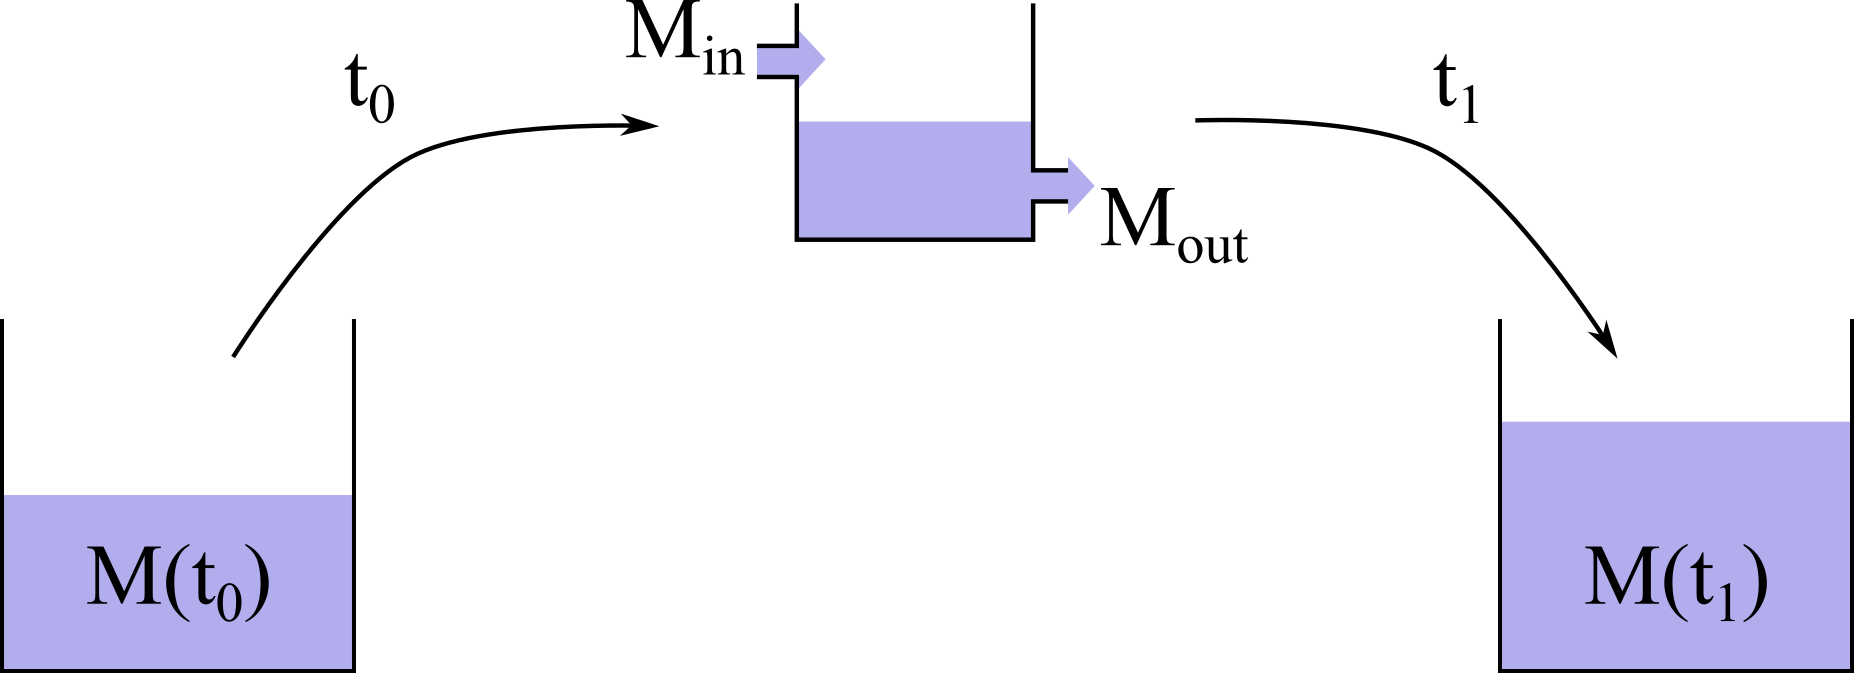
\includegraphics[width=\linewidth]{images/continuum_mechanics/massConservation.png}
	\caption[STAR mechanics: Mass conservation]{\label{fig:massConservation} Mass conservation. $M(t_{1}) = M(t_{0}) + M_{in} - M_{out}$}
\end{figure}
\\
Mathematically, we can write the conservation of mass as
\begin{equation}
    \label{eq:massConservation}
    \displaystyle 
    \frac{d}{dt}\left( \int_{\mathcal{V}} \rho(t,\mathbf{x}) dv \right)
    =
    - \int_{\mathcal{\partial V}}\rho(t,\mathbf{x})\mathbf{v}(t,\mathbf{x}) \cdot \mathbf{n}(\mathbf{x}) ds
\end{equation}
where
\begin{itemize}
	\item $\rho(t,\mathbf{x})$ is the density at a point $\mathbf{x}$ and at a time $t$.
	\item $\mathbf{v}(t,\mathbf{x})$ is the velocity at a point $\mathbf{x}$ and at a time $t$.
	\item $\mathcal{V}$ is a small volume of the simulation domain $\Omega$.
	\item $\mathcal{\partial V}$ is the border of $\mathcal{V}$.
	\item $\mathbf{n}(\mathbf{x})$ is the normal outward of $\mathcal{V}$ on a point $\mathbf{x}$ of $\partial\mathcal{V}$.
\end{itemize}
This formulation involves an integral over the volume and its boundary.
When numerically solving this equation, it is simpler not to have to make the distinction between a small element of $\mathcal{V}$ and a small element of $\partial \mathcal{V}$.
By using Stokes' theorem, we have
\begin{equation}
\displaystyle 
\int_{\partial \mathcal{V}} \rho \mathbf{v} \cdot \mathbf{n} ds =
\int_{\mathcal{V}} \nabla \cdot \left( \rho \mathbf{v} \right) dv
\end{equation}
and we can rewrite Equation~\eqref{eq:massConservation} as a single integral over $\mathcal{V}$
\begin{equation}
\label{eq:volumetricMassConservation}
\displaystyle 
\int_{\mathcal{V}} 
\left( \frac{\partial \rho}{\partial t} + \nabla \cdot \left( \rho  \mathbf{v} \right) \right) dv = \mathbf{0}
\end{equation}

\subsubsection{Conservation of momentum}
\label{subsubsec:starMechanics_momentumConservation}
The conservation of momentum is implied by Newton's second law which states that the forces applied on an object result into an acceleration which is inversely proportional to the mass of the object.
Figure~\ref{fig:momentumConservation} illustrates this law in the case of two balls on which a same force is applied.
The acceleration induced by the force is more important for the small ball which has a mass less important than the big ball.
\begin{figure}[!h]
\centering
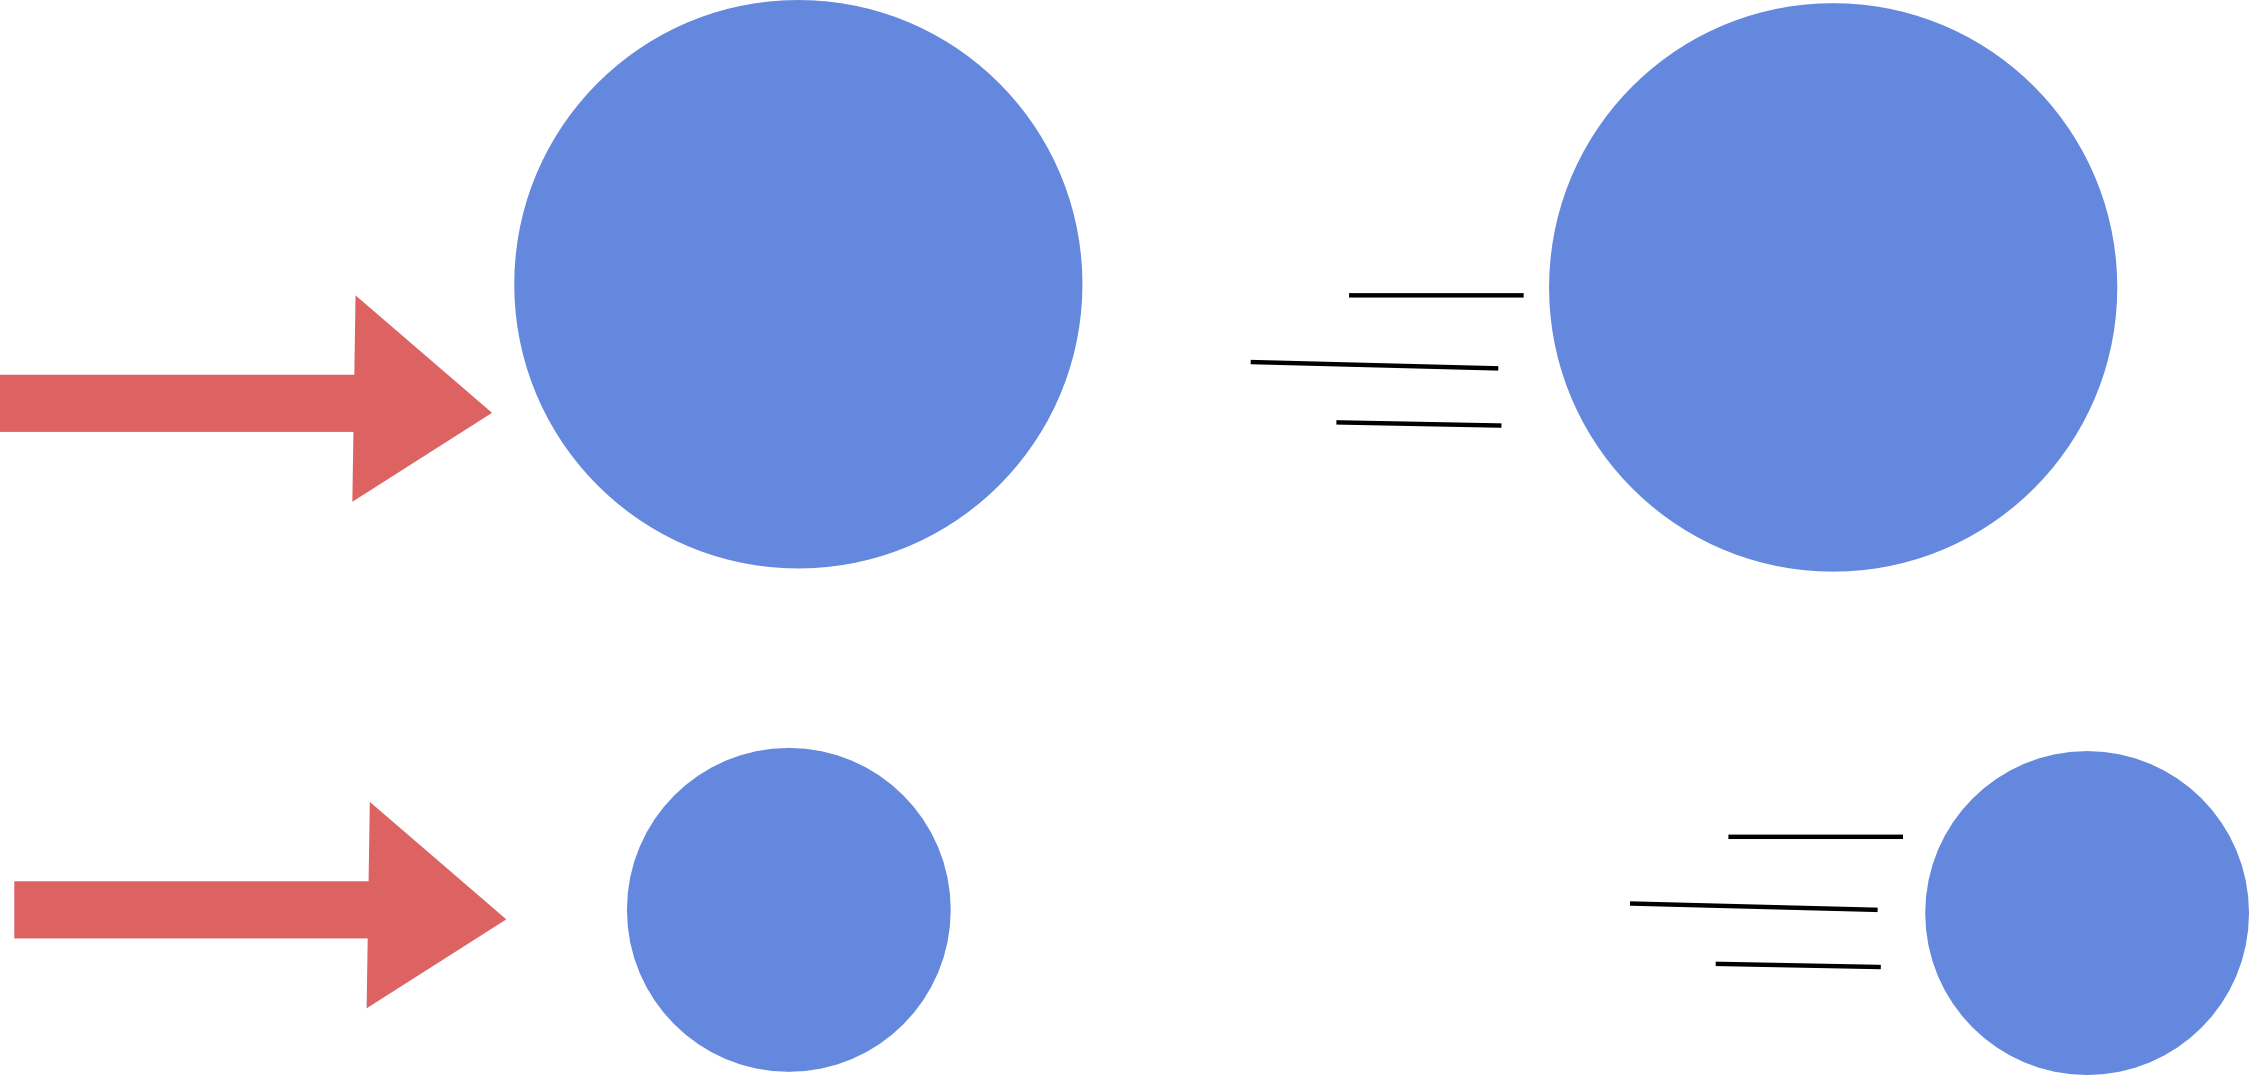
\includegraphics[width=\linewidth]{images/continuum_mechanics/momentumConservation.png}
\caption[STAR mechanics: Momentum conservation]{\label{fig:momentumConservation} Momentum conservation. The same force $\mathbf{f}$ is applied on two balls. The resulting acceleration is inversely proportional to their mass.}
\end{figure}
\\
Mathematically, this law can be written as
\begin{equation}
\displaystyle 
\int_{\mathcal{V}} 
\rho(t,\mathbf{x})\mathbf{a}(t,\mathbf{x}) dv 
= 
\int_{\mathcal{V}} \mathbf{f}(t,\mathbf{x}) dv
\end{equation}
where
\begin{itemize}
	\item $\mathbf{a}(t,\mathbf{x})$ is the acceleration at a point $\mathbf{x}$ and at a time $t$.
		\item $\mathbf{f}(t,\mathbf{x})$ is the force applied on a point $\mathbf{x}$ and at a time $t$.
\end{itemize}
By performing a Taylor-Young expansion on the acceleration, we can re-write the momentum conservation as
\begin{equation}
\label{eq:momentumConservation}
\displaystyle 
\int_{\mathcal{V}} 
\rho(t,\mathbf{x}) \left( \frac{\partial\mathbf{v}}{\partial t} + \mathbf{v} \cdot \nabla \mathbf{v} \right)(t,\mathbf{x}) dv 
= 
\int_{\mathcal{V}} \mathbf{f}(t,\mathbf{x}) dv
\end{equation}
Two kind of forces are generally applied on an object, the \emph{external} forces and the \emph{internal} forces.
External forces describe the action of the surrounding environment on the object. 
The simplest example is the weight, i.e. the force applied by the constant gravity $\mathbf{g}$ on the object:
\begin{equation}
\label{eq:externalForces}
\displaystyle \int_{\mathcal{V}} \mathbf{f}_{ext}(t,\mathbf{x})dv = \int_{\mathcal{V}} \rho(t,\mathbf{x}) \mathbf{g} dv
\end{equation}
Internal forces describe the reaction of the object to an external deformation.
Generally, they are defined by using a stress tensor $\sigma(t,\mathbf{x})$ as 
\begin{equation}
\displaystyle 
\int_{\mathcal{V}} \mathbf{f}_{int}(t,\mathbf{x}) dv 
= \int_{\partial \mathcal{V}} \sigma(t,\mathbf{x}) \mathbf{n}(\mathbf{x}) ds
\end{equation}
Basically, the stress relates the deformation of the object to its material properties by using a constitutive law.
A constitutive law is specific to the phenomena which is simulated.
In Section~\ref{subsec:fluidMechanics} and Section~\ref{subsec:solidMechanics}, we will respectively describe the most common constitutive laws for incompressible fluids and solids.
For a detailed and intuitive definition of the stress tensor we refer the reader to the \emph{SIGGRAPH} course about real-time physics~\cite{Muller2008} by M\"{u}ller et al.
\\
Same as for the conservation of mass, we can use Stokes' theorem to get a single integral over $\mathcal{V}$,
\begin{equation}
\label{eq:internalForces}
\displaystyle 
\int_{\mathcal{V}} \mathbf{f}_{int}\left(t,\mathbf{x}\right) dv 
\int_{\mathcal{V}} \nabla \cdot \sigma\left(t,\mathbf{x}\right) dv
\end{equation}
and we can rewrite Equation~\eqref{eq:momentumConservation} as
\begin{equation}
\label{eq:volumetricMomentumConservation}
\displaystyle
\int_{\mathcal{V}} 
\left( 
\rho \left( \frac{\partial\mathbf{v}}{\partial t} + \mathbf{v} \cdot \nabla \mathbf{v} \right)
- \nabla \cdot \sigma - \rho \mathbf{g}  \right) dv = \mathbf{0}
\end{equation}

\subsubsection{Eulerian vs. Lagrangian formulations}
\label{subsubsec:starMechanics_eulerianLagrangian}
Eulerian and Lagrangian formulations are two different ways of interpreting the equations of motion.
To understand the key difference, we take the example of the simulation of a river and use Figure~\ref{fig:EulerianVsLagrangian} to illustrate it.
Let us suppose that we want to measure fluid properties such as velocity, density or temperature of the river.
A first possibility would be to measure it at a fixed location, similarly to a buoy that would remain at the same spot and measures data at regular intervals of time. This is the Eulerian viewpoint. A second possibility is to measure it along a path that would follow the flow of the river, similarly to an object floating on the river or a particle of water moving accordingly to the flow. This is the Lagrangian viewpoint.
\begin{figure}[!ht]
	\centering
	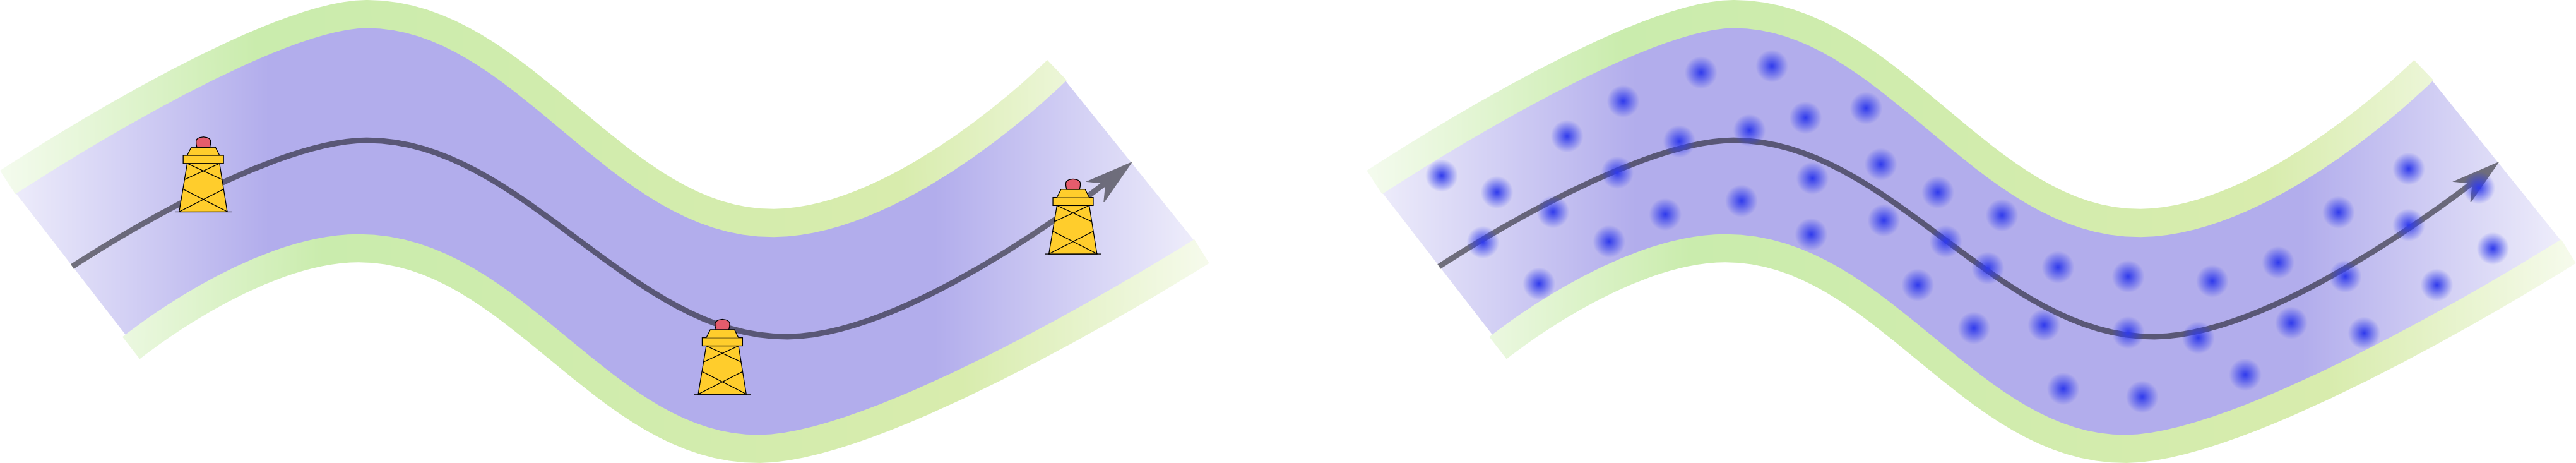
\includegraphics[width=\linewidth]{images/continuum_mechanics/eulerianVsLagrangian.png}
	\caption[STAR mechanics: Eulerian vs. Lagrangian]{\label{fig:EulerianVsLagrangian} Eulerian vs. Lagrangian viewpoint. On the left, buoys are put at fixed positions on a river and measure properties such as velocity, temperature, etc. The Eulerian approach takes a similar approach. On the right, we represent the river with particles of water which follows the flow of the river and carry properties with them. This is similar to the Lagrangian viewpoint.}
\end{figure}
Equation~\eqref{eq:volumetricMassConservation} and Equation~\eqref{eq:volumetricMomentumConservation} are described for fixed locations. Put together, they define the equations of motion from an Eulerian viewpoint.
\begin{equation}
\label{eq:eulerianMotionEquation}
\left\lbrace
\begin{array}{l}
\displaystyle 
\int_{\mathcal{V}} 
\left( 
\rho \left( \frac{\partial\mathbf{v}}{\partial t} + \mathbf{v} \cdot \nabla \mathbf{v} \right)
- \nabla \cdot \sigma - \rho \mathbf{g}  \right) dv = \mathbf{0}
\\ \\
\displaystyle
\int_{\mathcal{V}} 
\left( \frac{\partial \rho}{\partial t} + \nabla \cdot \left( \rho  \mathbf{v} \right) \right) dv = 0
\end{array}
\right.
\end{equation}
In order to adopt the Lagrangian viewpoint, let us suppose that the fluid properties are carried by particles and that $q(t,\mathbf{x})$ denote one of this property at a time $t$ for a particle which is at a position $\mathbf{x}$. 
If we want to compute the derivative of $q$ for the particle at position $\mathbf{x}$, we have to use the total derivative:
\begin{equation}
\label{eq:totalDerivative}
\frac{dq(t,\mathbf{x})}{dt} = 
\frac{\partial q}{\partial t}\cdot\frac{dt}{dt} + \frac{\partial q}{\partial \mathbf{x}} \cdot \frac{d\mathbf{x}}{dt} 
= \frac{\partial q}{\partial t}(t,\mathbf{x}) + \left(\nabla q(t,\mathbf{x}) \cdot \mathbf{v}\right)(t,\mathbf{x})
\end{equation}
In Equation~\eqref{eq:volumetricMomentumConservation} which describes the momentum conservation, we can directly use Equation~\eqref{eq:totalDerivative} to adopt a Lagrangian viewpoint. 
For the mass conservation described in Equation~\eqref{eq:volumetricMassConservation}, we first need to develop the divergence of the product between density and velocity and then Equation~\eqref{eq:totalDerivative} can be used.
Finally, we can write the equations of motion from a Lagrangian viewpoint as
\begin{equation}
\label{eq:lagrangianMotionEquation}
\left\lbrace
\begin{array}{l}
\displaystyle 
\int_{\mathcal{V}} 
\left( 
\rho \frac{d\mathbf{v}}{dt}
- \nabla \cdot \sigma - \rho \mathbf{g}  \right) dv = \mathbf{0}
\\ \\
\displaystyle
\int_{\mathcal{V}} 
\left( \frac{d\rho}{dt} + \rho \nabla \cdot \mathbf{v} \right) dv = 0
\end{array}
\right.
\end{equation}
As the deformable models used in Chapter~\ref{chap:arps} and Chapter~\ref{chap:cutting} are used to solve Lagrangian equations of motion, we will keep Equation~\eqref{eq:lagrangianMotionEquation} in the following sections.
\subsubsection{Numerical solution}
\label{subsubsec:starMechanics_numericalSolution}
Once the equations of motion are stated, they are discretized in space and time in order to be numerically solved.

\paragraph{Spatial discretization}
The spatial discretization consists in approximating the object to simulate using a finite number of samples. 
These samples carry the \emph{degrees of freedom} used to numerically solve the equations of motion.
Then, by using an \emph{interpolation method}, it is possible to approximate continuous quantities such as position, velocity, density and so on, at any location on the domain. 
Finally, an integration rule, also called \emph{quadrature rule}, is needed in order to integrate these quantities over the domain. 
These are the main components for solving the equations of motion:
degrees of freedom, an interpolation method and a quadrature rule for the numerical integration over the simulation domain.
\\ \\
There are multiple possibilities for these components. It is crucial to choose them based on the goals of the simulation: What do we want to measure ? How will boundaries be represented ? Will any topological changes occur ? Are there restrictions in terms of computational or memory cost ? In the following we briefly introduce the most commonly used solutions in Computer Graphics.

\subparagraph{Degrees of freedom}
In Eulerian simulation, velocities are the most common independent degrees of freedom while Lagrangian simulations generally use positions and velocities. 
We can also mention the use of affine frames to capture translations, rotations and shearing. They are used in the frame-based model which will be detailed in Section~\ref{subsubsec:framebased}.
\\ 
Usually, we distinguish two types of sampling of the degrees of freedom: mesh-based and mesh-less (see Figure~\ref{fig:discretization}).
\begin{figure}[!h]
	\centering
	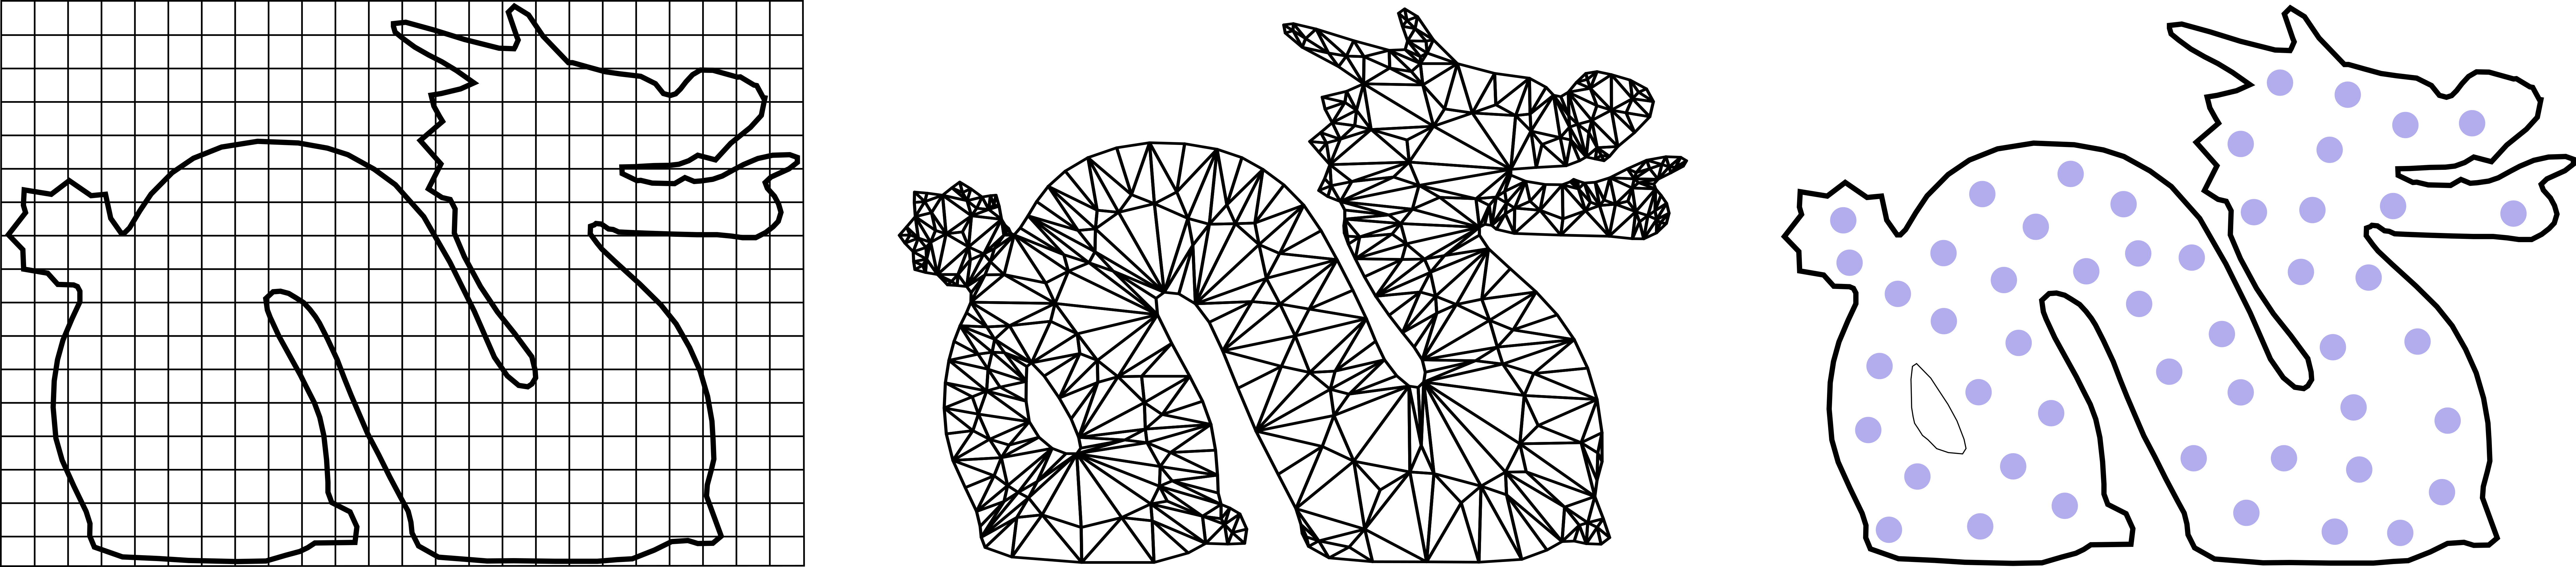
\includegraphics[width=\linewidth]{images/continuum_mechanics/discretization.png}
	\caption[STAR mechanics: Discretization]{\label{fig:discretization} On the left a grid discretization, commonly used in Eulerian simulations. In the middle an unstructured mesh discretization, commonly used in mesh-based Lagrangian simulations. On the right, a point-based discretization, commonly used in mesh-less Lagrangian simulations.}
\end{figure}
\\
In mesh-based methods, the vertices of a mesh are used to sample the degrees of freedom. For instance, Eulerian simulations usually use a cartesian grid which allows to accurately compute derivatives. 
In contrast, Lagrangian simulations are mostly based on unstructured triangular meshes which allows to handle complex boundaries.
In mesh-less methods, the samples are uniformly distributed over the domain. Depending on the simulated phenomena, the structure may be quasi-nonexistent which brings a lot of flexibility. For fluids, the neighborhood of the samples will change every time whereas for elastic solids their neighborhood will remain the same as long as the object does not undergo topological changes such as fracture or cutting.
Of course, each of these samplings can benefit from adaptivity. We will detail the different possibilities of spatial adaptivity in Chapter~\ref{chap:starAdaptivity}.

\subparagraph{Interpolation}
Interpolation is used to approximate the physical quantities over the domain such as density, displacement, pressure and so on. 
In Computer Graphics, we can distinguish two major interpolation methods: polynomial interpolation and kernel interpolation.
For each of them, different weights are used, as illustrated in Figure~\ref{fig:shapefunction}. The weights are also called \emph{shape functions} and can be seen as the region of influence of a sample.
\begin{figure}[!h]
	\centering
	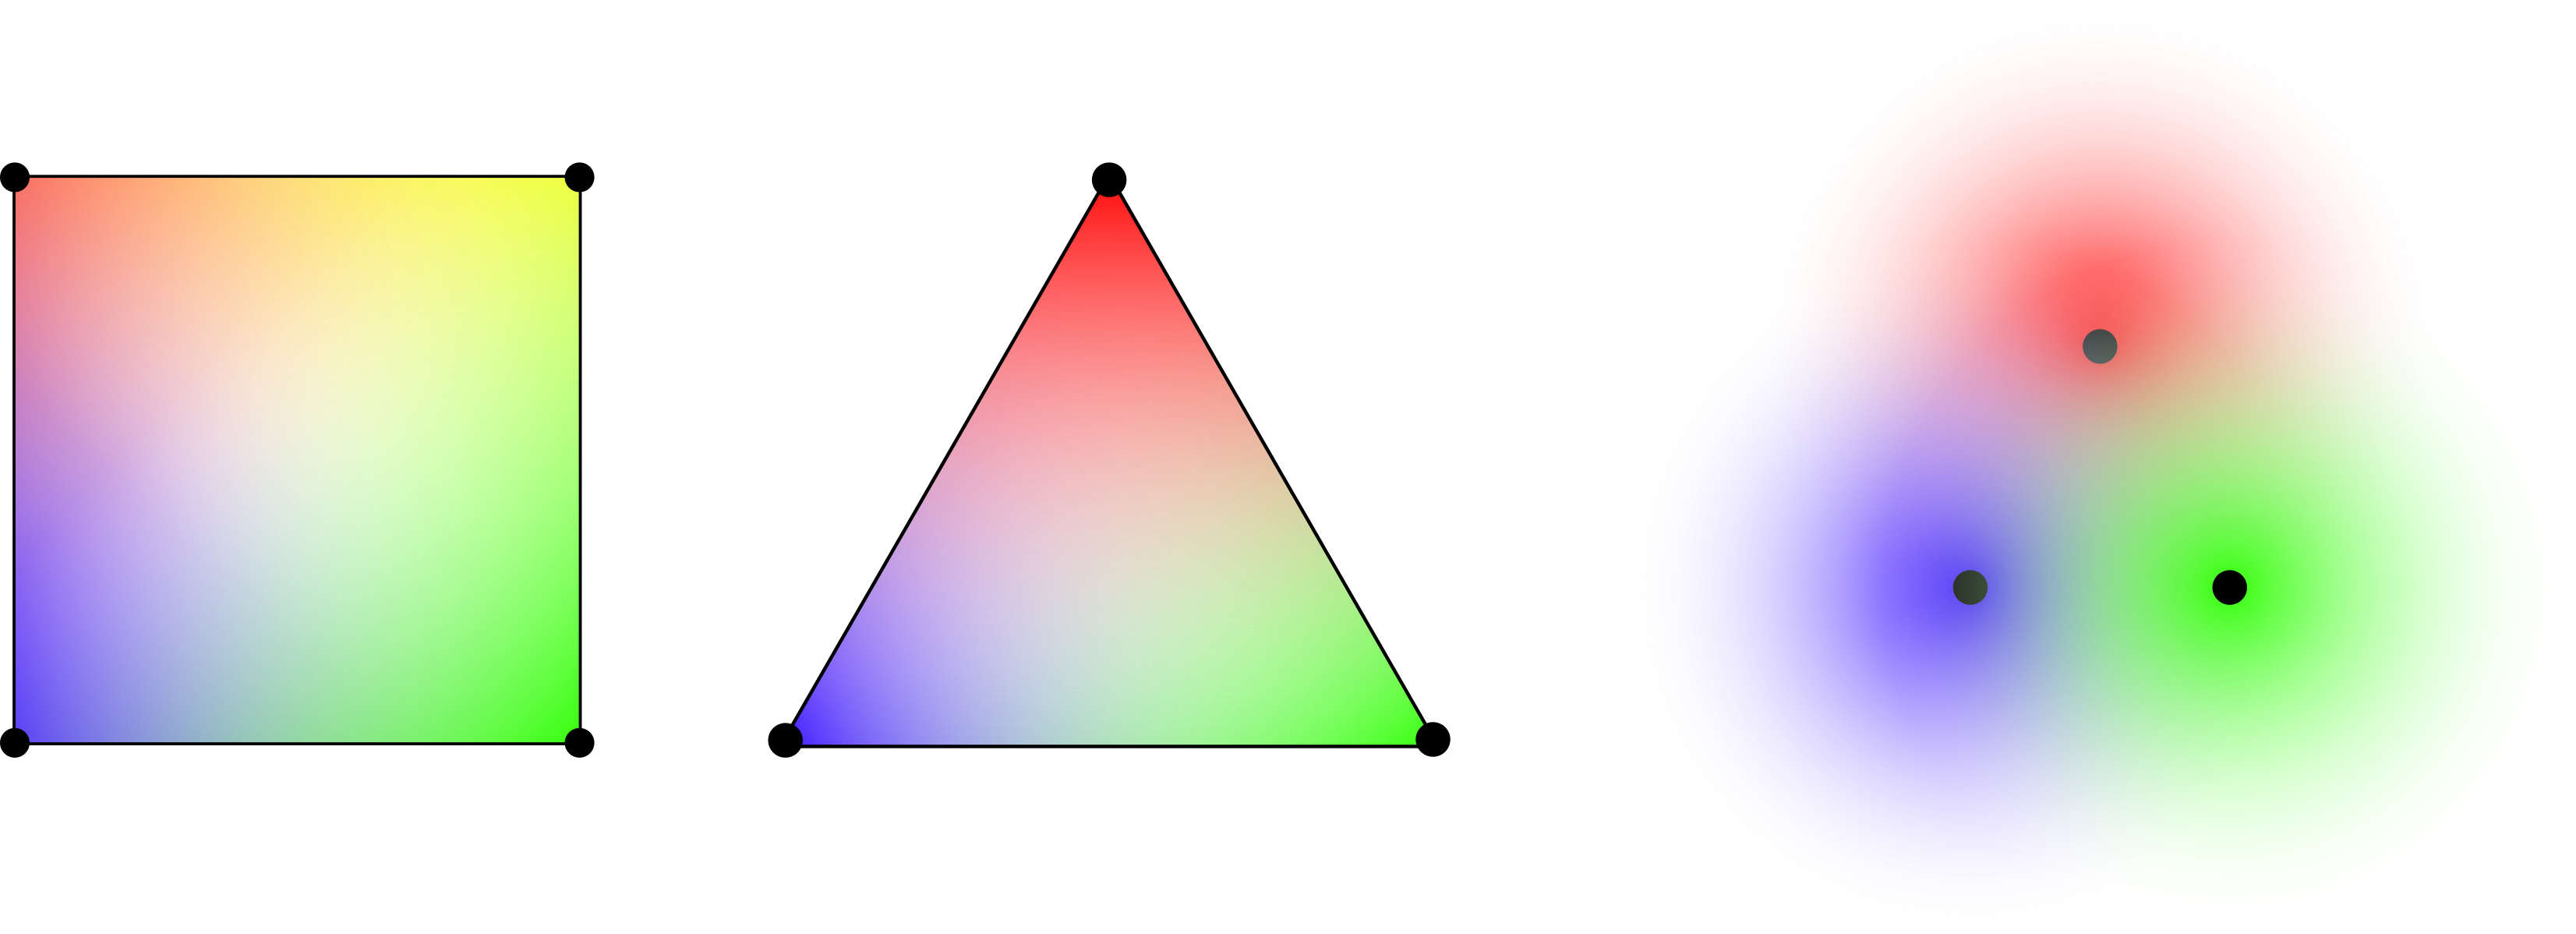
\includegraphics[width=\linewidth]{images/continuum_mechanics/shapefunction.png}
	\caption[STAR mechanics: Shape functions]{\label{fig:shapefunction} 
		Three examples of shape functions in 2D. 
		Each color represents the shape function associated to one sample point~(black circle) carrying the degrees of freedom. 
		On the left, shape functions for bilinear interpolation are illustrated. 
		In the middle, barycentric shape functions are illustrated. 
		On the right, kernel-based shape functions that are used in SPH and MLS interpolation are illustrated.}
\end{figure}
\\
The choice of the interpolation method mainly depends on how the material samples have been distributed. 
For a sampling based on cartesian grid, trilinear interpolation is often used, for instance in Eulerian simulations~\cite{Bridson2008}. 
For unstructured triangle meshes, linear interpolation with barycentric weights is the most popular choice to simulate elastic solids~\cite{Muller2008}.
For mesh-less samplings, the two most common kernel interpolation methods are Smoothed-Particles Hydrodynamics (SPH) interpolation and Moving Least Squares (MLS) interpolation.
SPH interpolation has been used to simulate a wide range of phenomena from fluid~\cite{Desbrun1999} to elastic solids~\cite{Becker2009}.
MLS has been introduced by M\"{u}ller et al. to simulate elastic and plastic deformations~\cite{Muller2004:melting}.
It was later extended to solids fracture by Pauly et al.~\cite{Pauly2005} and interactive cutting by Steinemann et al.~\cite{Steinemann2009}.
Both methods require a dense sampling of th object and can be used using a cubic kernel as shape function. We will provide more details about SPH and its use for the simulation of incompressible fluid in Section~\ref{subsubsec:starSPH} and how to save computational time by using an adaptive model in Section~\ref{sec:arps_sph}.
\\
Of course, mesh-based and mesh-less methods can be combined to get the best of both worlds.
In this case, two interpolation methods are used, one for the mesh-based side and one for the mesh-less side.
We refer the reader to the recent \emph{SIGGRAPH} course on the material point method~\cite{Jiang2016}.
In this course, existing hybrid models are compared and the interpolation methods to transfer data from one representation  to another are described.
\\
A common drawback of the methods mentioned above is that they require a dense sampling. In Section~\ref{sec:adaptivesf}, we will detail how to interactively handle topological changes with a sparse sampling by using the Voronoi-based interpolation method used in the frame-based model.

\subparagraph{Spatial Integration}

Over the simulation, different physical quantities such as density or internal forces, need to be integrated over the domain. 
There is need for a quadrature rule. 
Many exist, most of the time the simple midpoint rule is chosen (see Figure~\ref{fig:spatialIntegration}). 
\begin{figure}[!h]
	\centering
	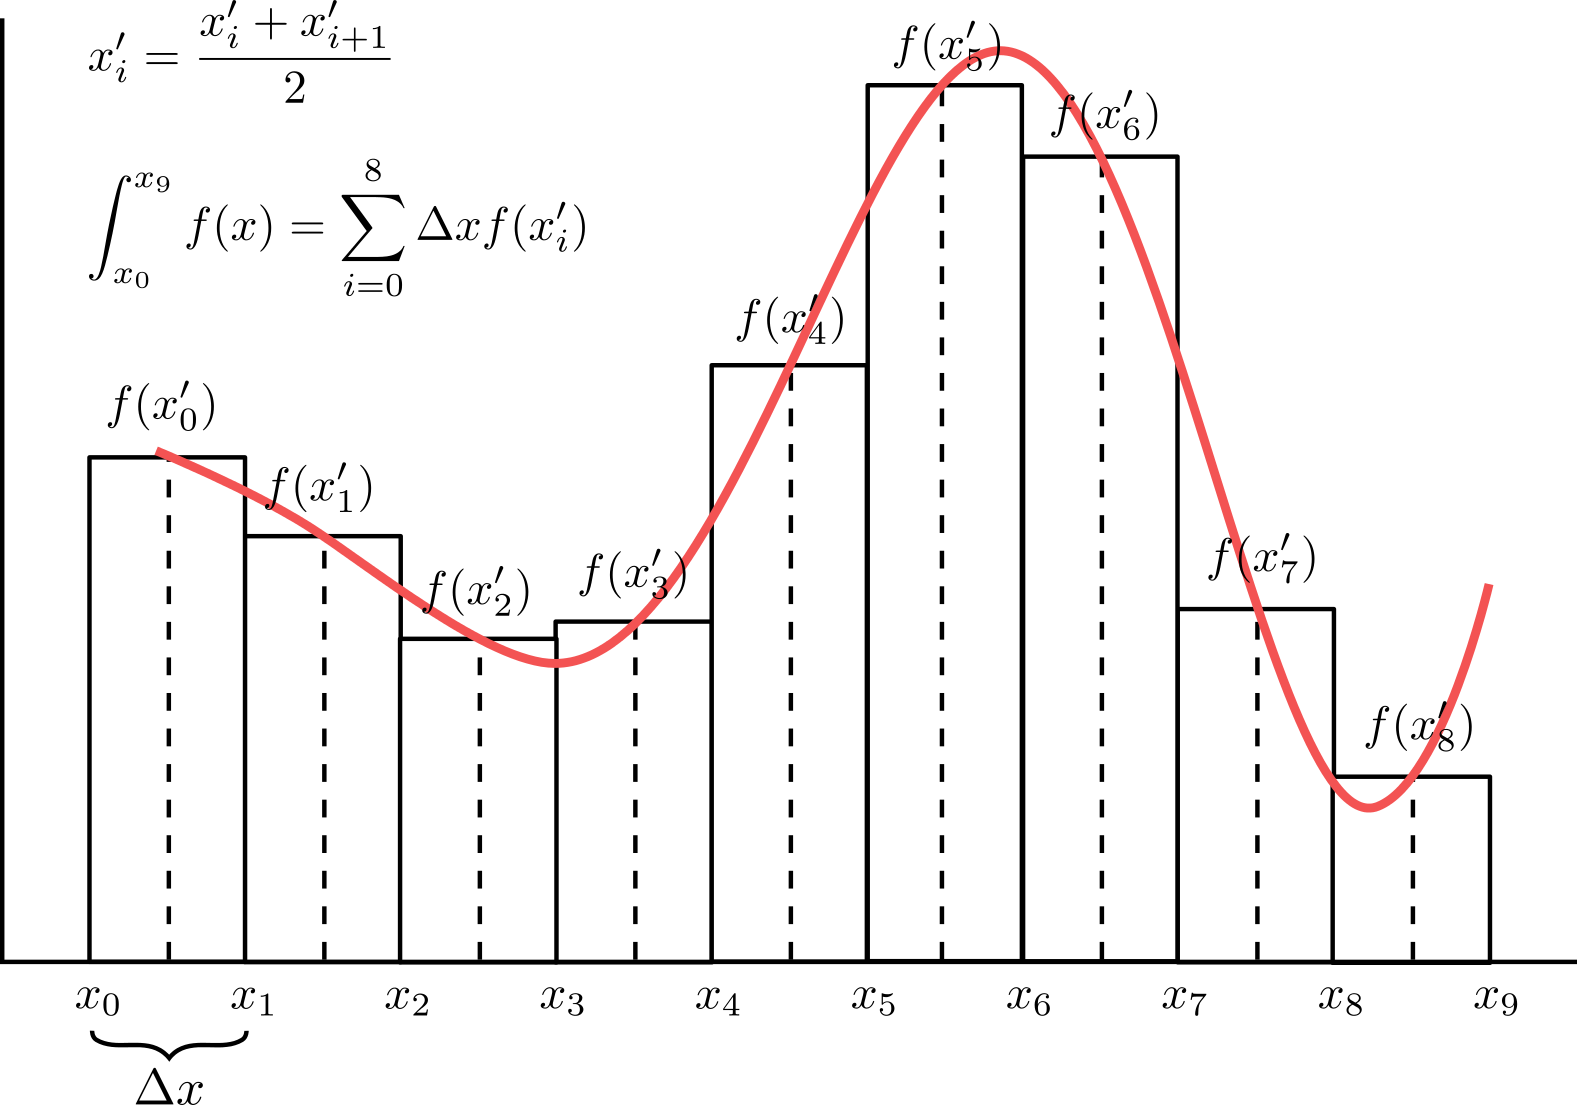
\includegraphics[width=\linewidth]{images/continuum_mechanics/spatialIntegration.png}
	\caption[STAR mechanics: Spatial integration]{\label{fig:spatialIntegration} Illustration of the midpoint rule for a one dimensional function. The integration domain is partitioned into uniform regions $\left[x_{i}, x_{i+1}\right]$, an integration point $x'_{i}$ is sampled at the center of each partition and the function is evaluated at the location of the integration points.}
\end{figure}
\\
The domain is decomposed in a set of partitions, where each partition has an associated volume $V_{i}$. 
\emph{Mid}-Points $\mathbf{x'}_{i}$ are sampled at the center of each partition.
They are called \emph{integration points}. 
Then the integral of a function $f$ over a domain $\Omega$ is approximated by:
\begin{equation}
\label{eq:midpointRule}
\int_{\Omega} f(\mathbf{x})dv \simeq \sum_{i} V_{i}f(\mathbf{x'}_{i})
\end{equation}
In mesh-based methods, it is common to consider one integration point at the center of each element and integrate over the volume of the element.
In mesh-less methods, when the sampling is dense, integration points are often co-located with the material samples and integrated over their associated volume. 
However, when the sampling is sparse, an independent sampling of integration points can be used to get a finer integration.
This is the case in the frame-based method that will be described in Section~\ref{subsubsec:framebased}.

\paragraph{Time integration}
Let us assume that we spatially discretized the Lagrangian equations of motion, Equation~\eqref{eq:lagrangianMotionEquation}, using a finite number of samples $N$ which carry positions and velocities as degrees of freedom.
For the sake of simplicity, we also assume that each sample has a fixed mass through the simulation which implies that mass conservation is ensured. Then, we can solely focus on the conservation of momentum and its integration over the time range  $\left[0, T\right]$ of the simulation. 
\\ \\
As for spatial integration, the temporal domain is discretized. Ideally, this discretization would adapt to the time scale of the simulation. For instance, fast motion would require a fine discretization while a coarse discretization would be sufficient for slow motion. We will detail the different techniques for an adaptive discretization of time in Section~\ref{sec t adaptivity}.
In the following, we simply assume a uniform discretization of $\left[0,T\right]$ defined by a time step $\Delta t$. The integration between two consecutive time steps $t_{n}$ and $t_{n+1}$ can be written as
\begin{equation}
\label{eq:timeIntegration1}
\displaystyle
\int_{t_{n}}^{t_{n+1}}
M \frac{d\mathbf{v}}{dt} dt
=
\int_{t_{n}}^{t_{n+1}}\mathbf{f} dt
\end{equation}
where
\begin{itemize}
	\item $\mathbf{v} \in \mathbb{R}^{3N}$ concatenates the velocity of each sample.
	\item $\mathbf{f} \in \mathbb{R}^{3N}$ concatenates the forces applied on each sample.
	\item $M \in \mathbb{R}^{3N \times 3N}$ concatenates the mass of each sample.
\end{itemize}
Many integration schemes can be used. Most of them can be explained using the Taylor expansion of a function $f$,
\begin{equation}
\label{eq:taylorExpansion}
\displaystyle
f(x) = \sum_{\alpha=0}^{k}\frac{\left(x-a\right)^{\alpha}}{\alpha!}f^{(\alpha)}(a) + \int_{a}^{x}\frac{\left(x-t\right)^{k}}{k!}f^{(k+1)}(t)dt
\end{equation}
By applying Equation~\eqref{eq:taylorExpansion} on $\mathbf{v}$ with $k=0$, we have
\begin{equation}
\mathbf{v}(t_{n+1}) = \mathbf{v}(t_{n}) + \int_{t_{n}}^{t_{n+1}} \frac{d\mathbf{v}}{dt}dt
\end{equation}
which allows to rewrite Equation~\eqref{eq:timeIntegration1} as
\begin{equation}
\label{eq:timeIntegration2}
\mathbf{v}(t_{n+1}) = \mathbf{v}(t_{n}) + \int_{t_{n}}^{t_{n+1}} M^{-1}\mathbf{f}dt
\end{equation}
This expression can be further expanded in order to get more accurate results. In Computer Graphics, this is the most used expansion. Finally, the integral term in Equation~\eqref{eq:timeIntegration2} is generally computed with the rectangle quadrature rule which we illustrate in Figure~\ref{fig:rectangleRules}.
\begin{figure}[!ht]
	\centering
	\begin{subfigure}[b]{0.46\linewidth}
		\centering
		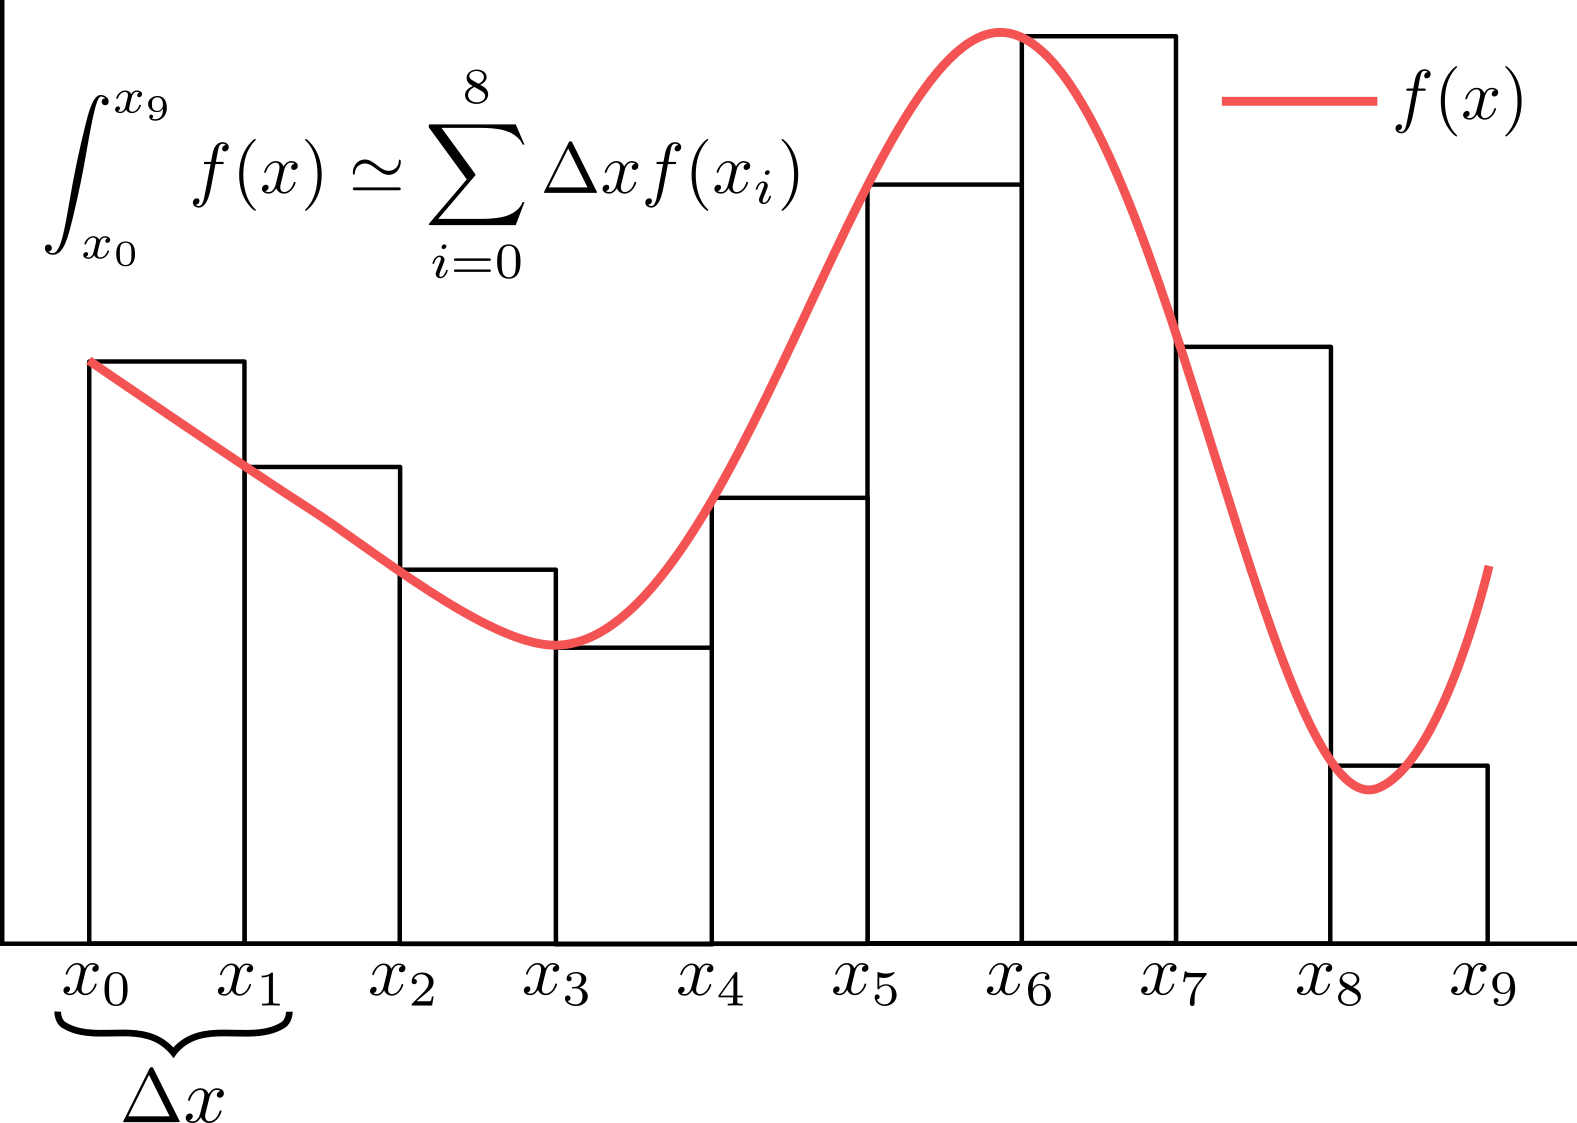
\includegraphics[width=\linewidth]{images/continuum_mechanics/rectangleRule_left.png}
		\caption{\label{fig:leftRectangleRule}}
	\end{subfigure}
	\hspace{0.2cm}
	\begin{subfigure}[b]{0.46\linewidth}
		\centering
		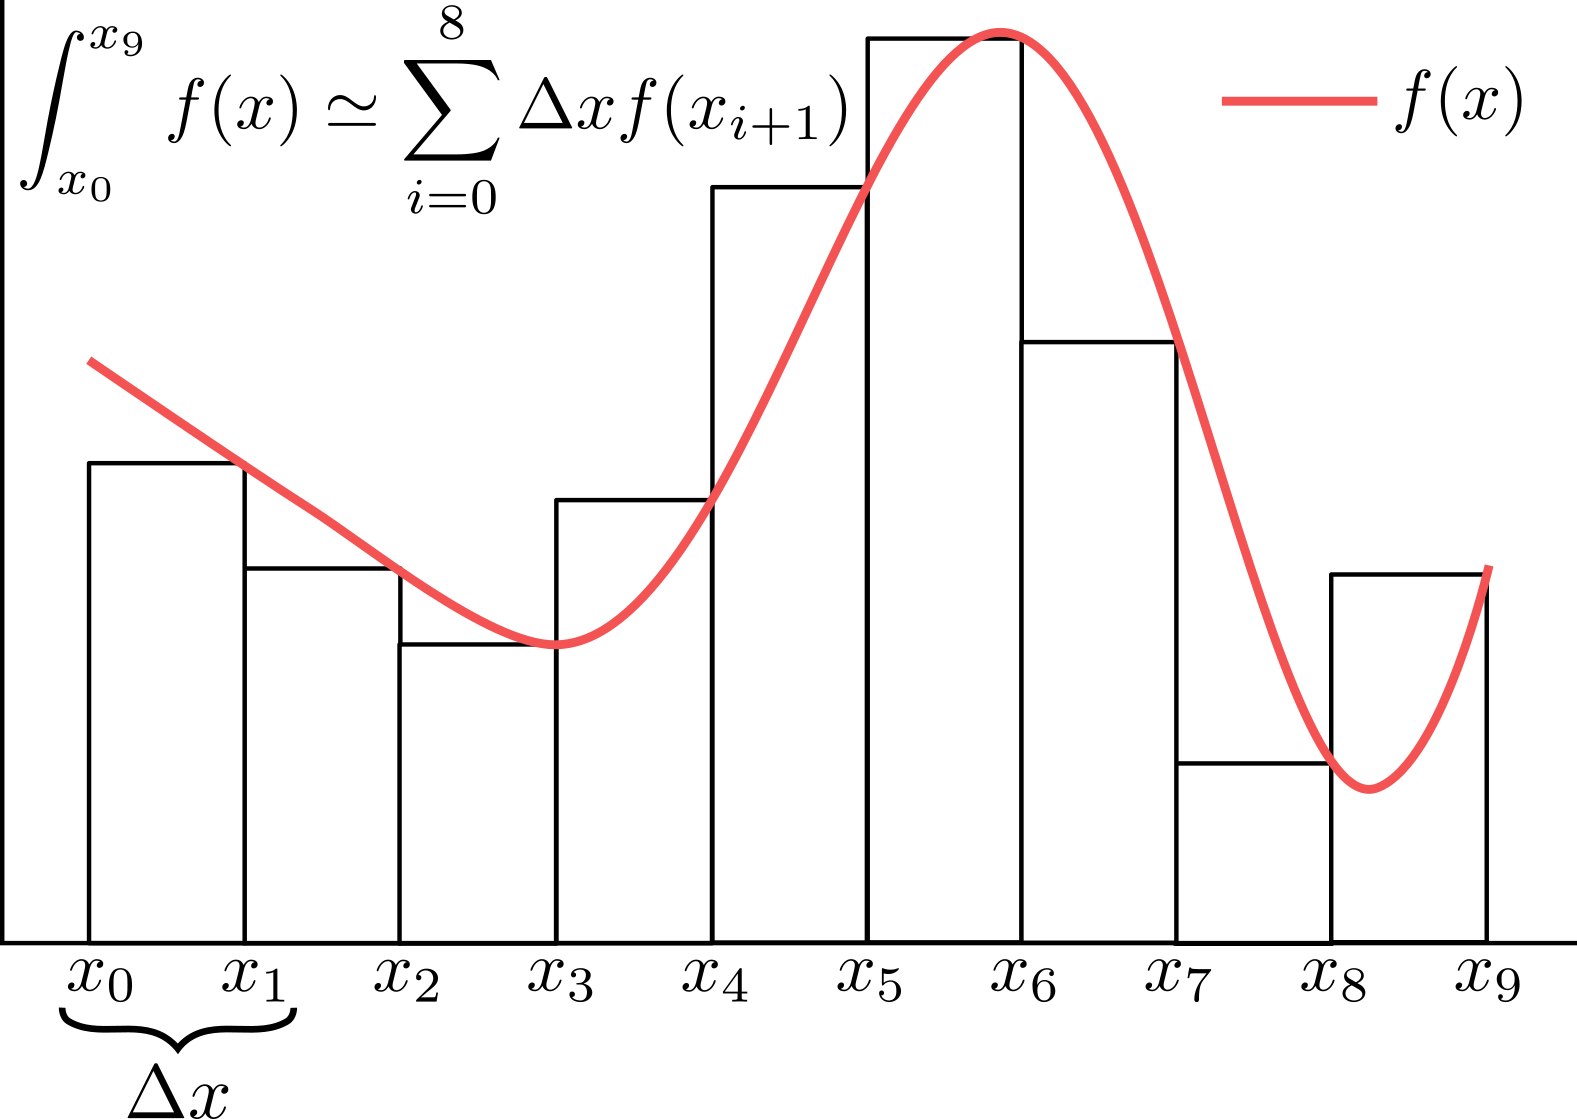
\includegraphics[width=\linewidth]{images/continuum_mechanics/rectangleRule_right.png}
		\caption{\label{fig:rightRectangleRule}}
	\end{subfigure}
	\caption[STAR mechanics: Rectangle integration rules]{\label{fig:rectangleRules}
		Illustrations of the rectangle integration rules. A function $f$ can be integrated over a regularly sampled domain using either the left rectangle rule~(a) or the right rectangle rule~(b).}
\end{figure}
\\
For a left rectangle method, we get an explicit integration of the velocity
\begin{equation}
\label{eq:explicitIntegration}
\mathbf{v}(t_{n+1}) = \mathbf{v}(t_{n}) + \Delta t M^{-1}\mathbf{f}(t_{n})
\end{equation}
For a right rectangle method, we get an implicit integration of the velocity
\begin{equation}
\label{eq:implicitIntegration}
\mathbf{v}(t_{n+1}) = \mathbf{v}(t_{n}) + \Delta t M^{-1}\mathbf{f}(t_{n+1})
\end{equation}
We can apply the same rule for the integration of the positions.
Depending on which quantity is integrated first and which integration rule is used, we can distinguish three main schemes used in computer graphics: forward Euler, symplectic Euler and backward Euler.
\begin{figure}[!ht]
	\centering
	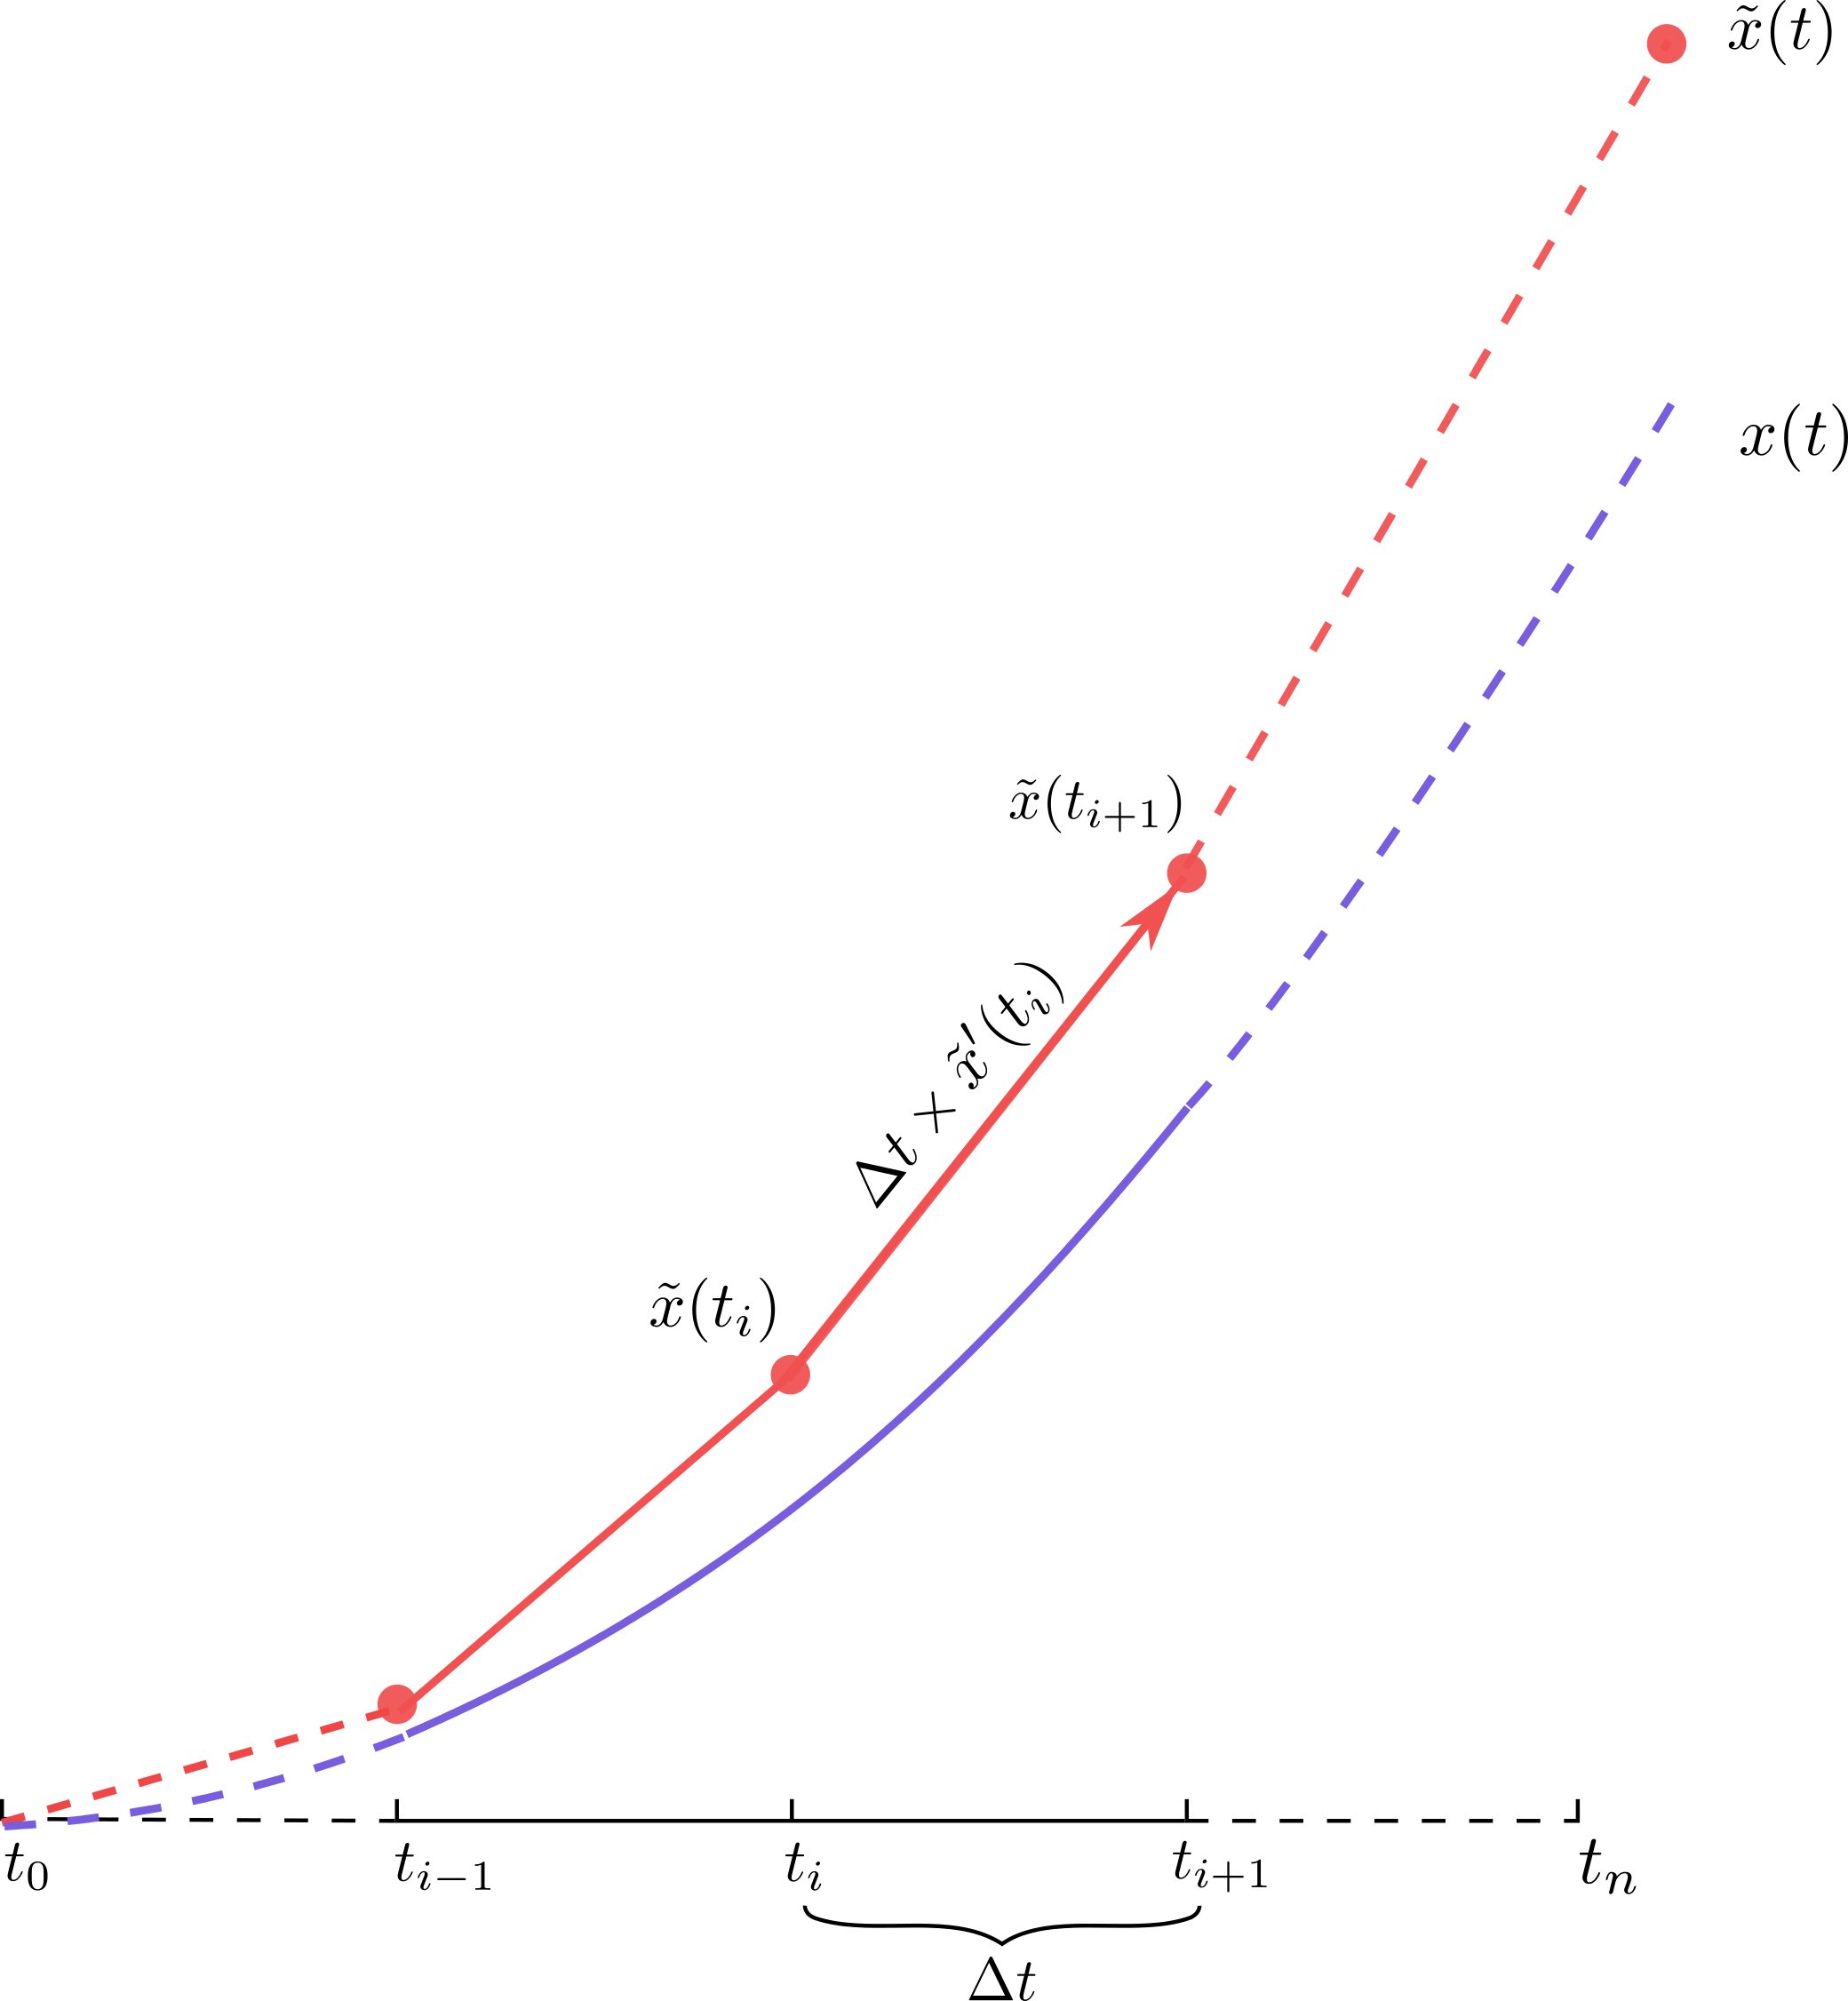
\includegraphics[scale=0.6]{images/continuum_mechanics/timeIntegration.png}
	\caption[STAR mechanics: Temporal integration]{\label{fig:timeIntegration} 
		Illustration of a 1D forward Euler time integration. 
		$x(t)$ describes the solution and $x'(t)$ describes the numerical approximation.}
\end{figure}
Forward Euler is the explicit integration of both position and velocity.
Figure~\ref{fig:timeIntegration} illustrates the integration of position in 1D,
\begin{equation}
\label{eq:explicitEuler}
\begin{array}{l}
\displaystyle \mathbf{x}(t_{n+1}) = \mathbf{x}(t_{n}) + \Delta t \mathbf{v}(t_{n}) \\ \\
\displaystyle \mathbf{v}(t_{n+1}) = \mathbf{v}(t_{n}) + \Delta t M^{-1}\mathbf{f}(t_{n})
\end{array}
\end{equation}
Symplectic Euler is the explicit integration of velocity and implicit integration of position,
\begin{equation}
\label{eq:symplecticEuler}
\begin{array}{l}
\displaystyle \mathbf{v}(t_{n+1}) = \mathbf{v}(t_{n}) + \Delta t M^{-1} \mathbf{f}(t_{n}) \\ \\
\displaystyle \mathbf{x}(t_{n+1}) = \mathbf{x}(t_{n}) + \Delta t \mathbf{v}(t_{n+1})
\end{array}
\end{equation}
Backward Euler is the implicit integration of both position and velocity,
\begin{equation}
\label{eq:backwardEuler}
\begin{array}{ll}
\displaystyle \mathbf{v}(t_{n+1}) = \mathbf{v}(t_{n}) + M^{-1}\Delta t \mathbf{f}(t_{n+1}) \\ \\
\displaystyle \mathbf{x}(t_{n+1}) = \mathbf{x}(t_{n}) + \Delta t \mathbf{v}(t_{n+1})
\end{array}
\end{equation}
Forward and symplectic Euler are among the easiest integration schemes. 
They are cheap and easy to implement. 
However, stability is guaranteed for a restricted range of time steps. 
Backward Euler is more expensive as it requires the solution of an equation. 
However unconditional stability is guaranteed which means that large time steps can be used resulting in a significant speed-up of the simulation. This speed-up comes at the price of numerical damping which might be undesired.
A nice way to solve the non-linear equation of backward Euler is to expand the force expression and linearize in order to fall back to solving a linear system. There, efficient iterative methods such as the conjugate gradient can be used.
In Section~\ref{sec:arps_implicit}, we describe the linear system resulting from the use of backward Euler and detail how to combine it with the adaptive method that we present in Chapter~\ref{chap:arps}.

\subsection{Fluid mechanics}
\label{subsec:fluidMechanics}
In this section, we describe a constitutive law for incompressible fluids such as water and we detail how to solve the equations of motion by using the Smoothed-Particle Hydrodynamics~(SPH) model that we will use in Section~\ref{sec:arps_sph}.
\subsubsection{Constitutive Law}
Fluids, for instance smoke, mainly react to pressure and viscosity.
The stress tensor that we introduced in Section~\ref{subsubsec:starMechanics_momentumConservation} is used to relate the deformation of the fluid to this two properties in the following constitutive law
\begin{equation}
\label{eq:fluidConstitutiveLaw}
\sigma = -pI + \eta \left( \nabla \mathbf{v} + \nabla \mathbf{v}^{T} \right)
\end{equation}
where
\begin{itemize}
	\item $p$ is the pressure applied on the fluid.
	\item $\eta$ is the viscosity of the fluid.
\end{itemize}
By injecting this equation into Equation~\eqref{eq:internalForces}, we get the internal forces of the fluid:
\begin{equation}
\label{eq:internalForces_liquids}
\mathbf{f}_{int} = \nabla \cdot \sigma = \nabla \cdot \left( -pI + \eta \left( \nabla \mathbf{v} + \nabla \mathbf{v}^{T} \right) \right) = -\nabla p + \Delta \mathbf{v}
\end{equation}
If we want to describe an incompressible fluid such as water, we need to specify that the mass should not vary over time which means
\begin{equation}
\label{eq:incompressibility}
\frac{d\rho}{dt} = 0
\end{equation}
By using Equation~\eqref{eq:internalForces_liquids}~and~\eqref{eq:incompressibility} in the equations of motion described in Equation~\eqref{eq:lagrangianMotionEquation}, we now describe an incompressible fluid. These new equations of motion are called the Navier-Stokes equations for an incompressible fluid
\begin{equation}
\label{eq:navierStokes}
\left\lbrace
\begin{array}{ll}
\displaystyle \int_{\mathcal{V}} \left( \rho \frac{d}{dt} \mathbf{v} + \nabla p - \eta \Delta \mathbf{v} - \rho \mathbf{g} \right)dv = \mathbf{0}\\ \\
\displaystyle \int_{\mathcal{V}} \nabla. \mathbf{v} = 0
\end{array}
\right.
\end{equation}
\subsubsection{Smoothed-Particles Hydrodynamics model}
\label{subsubsec:starSPH}
Smoothed-Particles Hydrodynamics (SPH) is an interpolation method that can be used to approximate Navier-Stokes equations in a Lagrangian way. SPH was initially proposed by Monaghan~\cite{Monaghan1992} and introduced in graphics by Desbrun et al.~\cite{Desbrun1999}.
The fluid is discretized into particles which represent small volumes of the whole fluid and each quantity carried by the particle is interpolated using SPH.

\paragraph{SPH interpolation}
The interpolation of a function $f$ and its derivatives of order $\alpha$ at a position $\mathbf{x}$ using SPH are defined as
\begin{equation}
\label{eq:sphInterpolation}
\left\lbrace
\begin{array}{l}
\displaystyle f(\mathbf{x}) = \int_{V} f(\mathbf{x'})W(\mathbf{x}-\mathbf{x'}, h)d\mathbf{x'} \\ \\
\displaystyle D^{\alpha} f(\mathbf{x}) = \int_{\mathcal{V}} f(\mathbf{x'}) D^{\alpha} W(\mathbf{x}-\mathbf{x'}, h)d\mathbf{x'}
\end{array}
\right.
\end{equation}
where 
\begin{itemize}
	\item $W$ is a function called \emph{kernel}.
	\item $h$ is the smoothing radius, also called length scale, which represents the support of $W$.
\end{itemize} 
Let assume that the fluid is discretized using $N$ particles.
These particles play two roles: First they carry the degrees of freedom and the fluid properties; Second their position are used as integration points. By applying the midpoint rule from Equation~\eqref{eq:midpointRule}, we get a discretized version of Equation~\eqref{eq:sphInterpolation}:
\begin{equation}
\label{eq:sphFunction}
\left\lbrace
\begin{array}{l}
\displaystyle f(\mathbf{x}) = \sum_{i=0}^{N} f(\mathbf{x}_{i})V_{i} W(\mathbf{x}-\mathbf{x}_{i},h) \\ \\
\displaystyle D^{\alpha} f(\mathbf{x})= \sum_{i=0}^{N} f(\mathbf{x}_{i})V_{i} D^{\alpha} W(\mathbf{x}-\mathbf{x}_{i},h)
\end{array}
\right.
\end{equation}
where 
\begin{itemize}
	\item $V_{i} = m_{i}/\rho_{i}$ is the volume of particle $i$.
	\item $m_{i}$ is the mass of particle $i$.
	\item $\rho_{i}$ is the density of particle $i$.
\end{itemize}
\paragraph{How to choose the kernel}
The choice of the kernel varies depending on the function to interpolate. In practice, the cubic kernel from Monaghan~\cite{Monaghan1992}~(Figure~\ref{fig:cubicKernel}) that we use in Chapter~\ref{chap:arps} works well.
\begin{figure}[H]
	\centering
	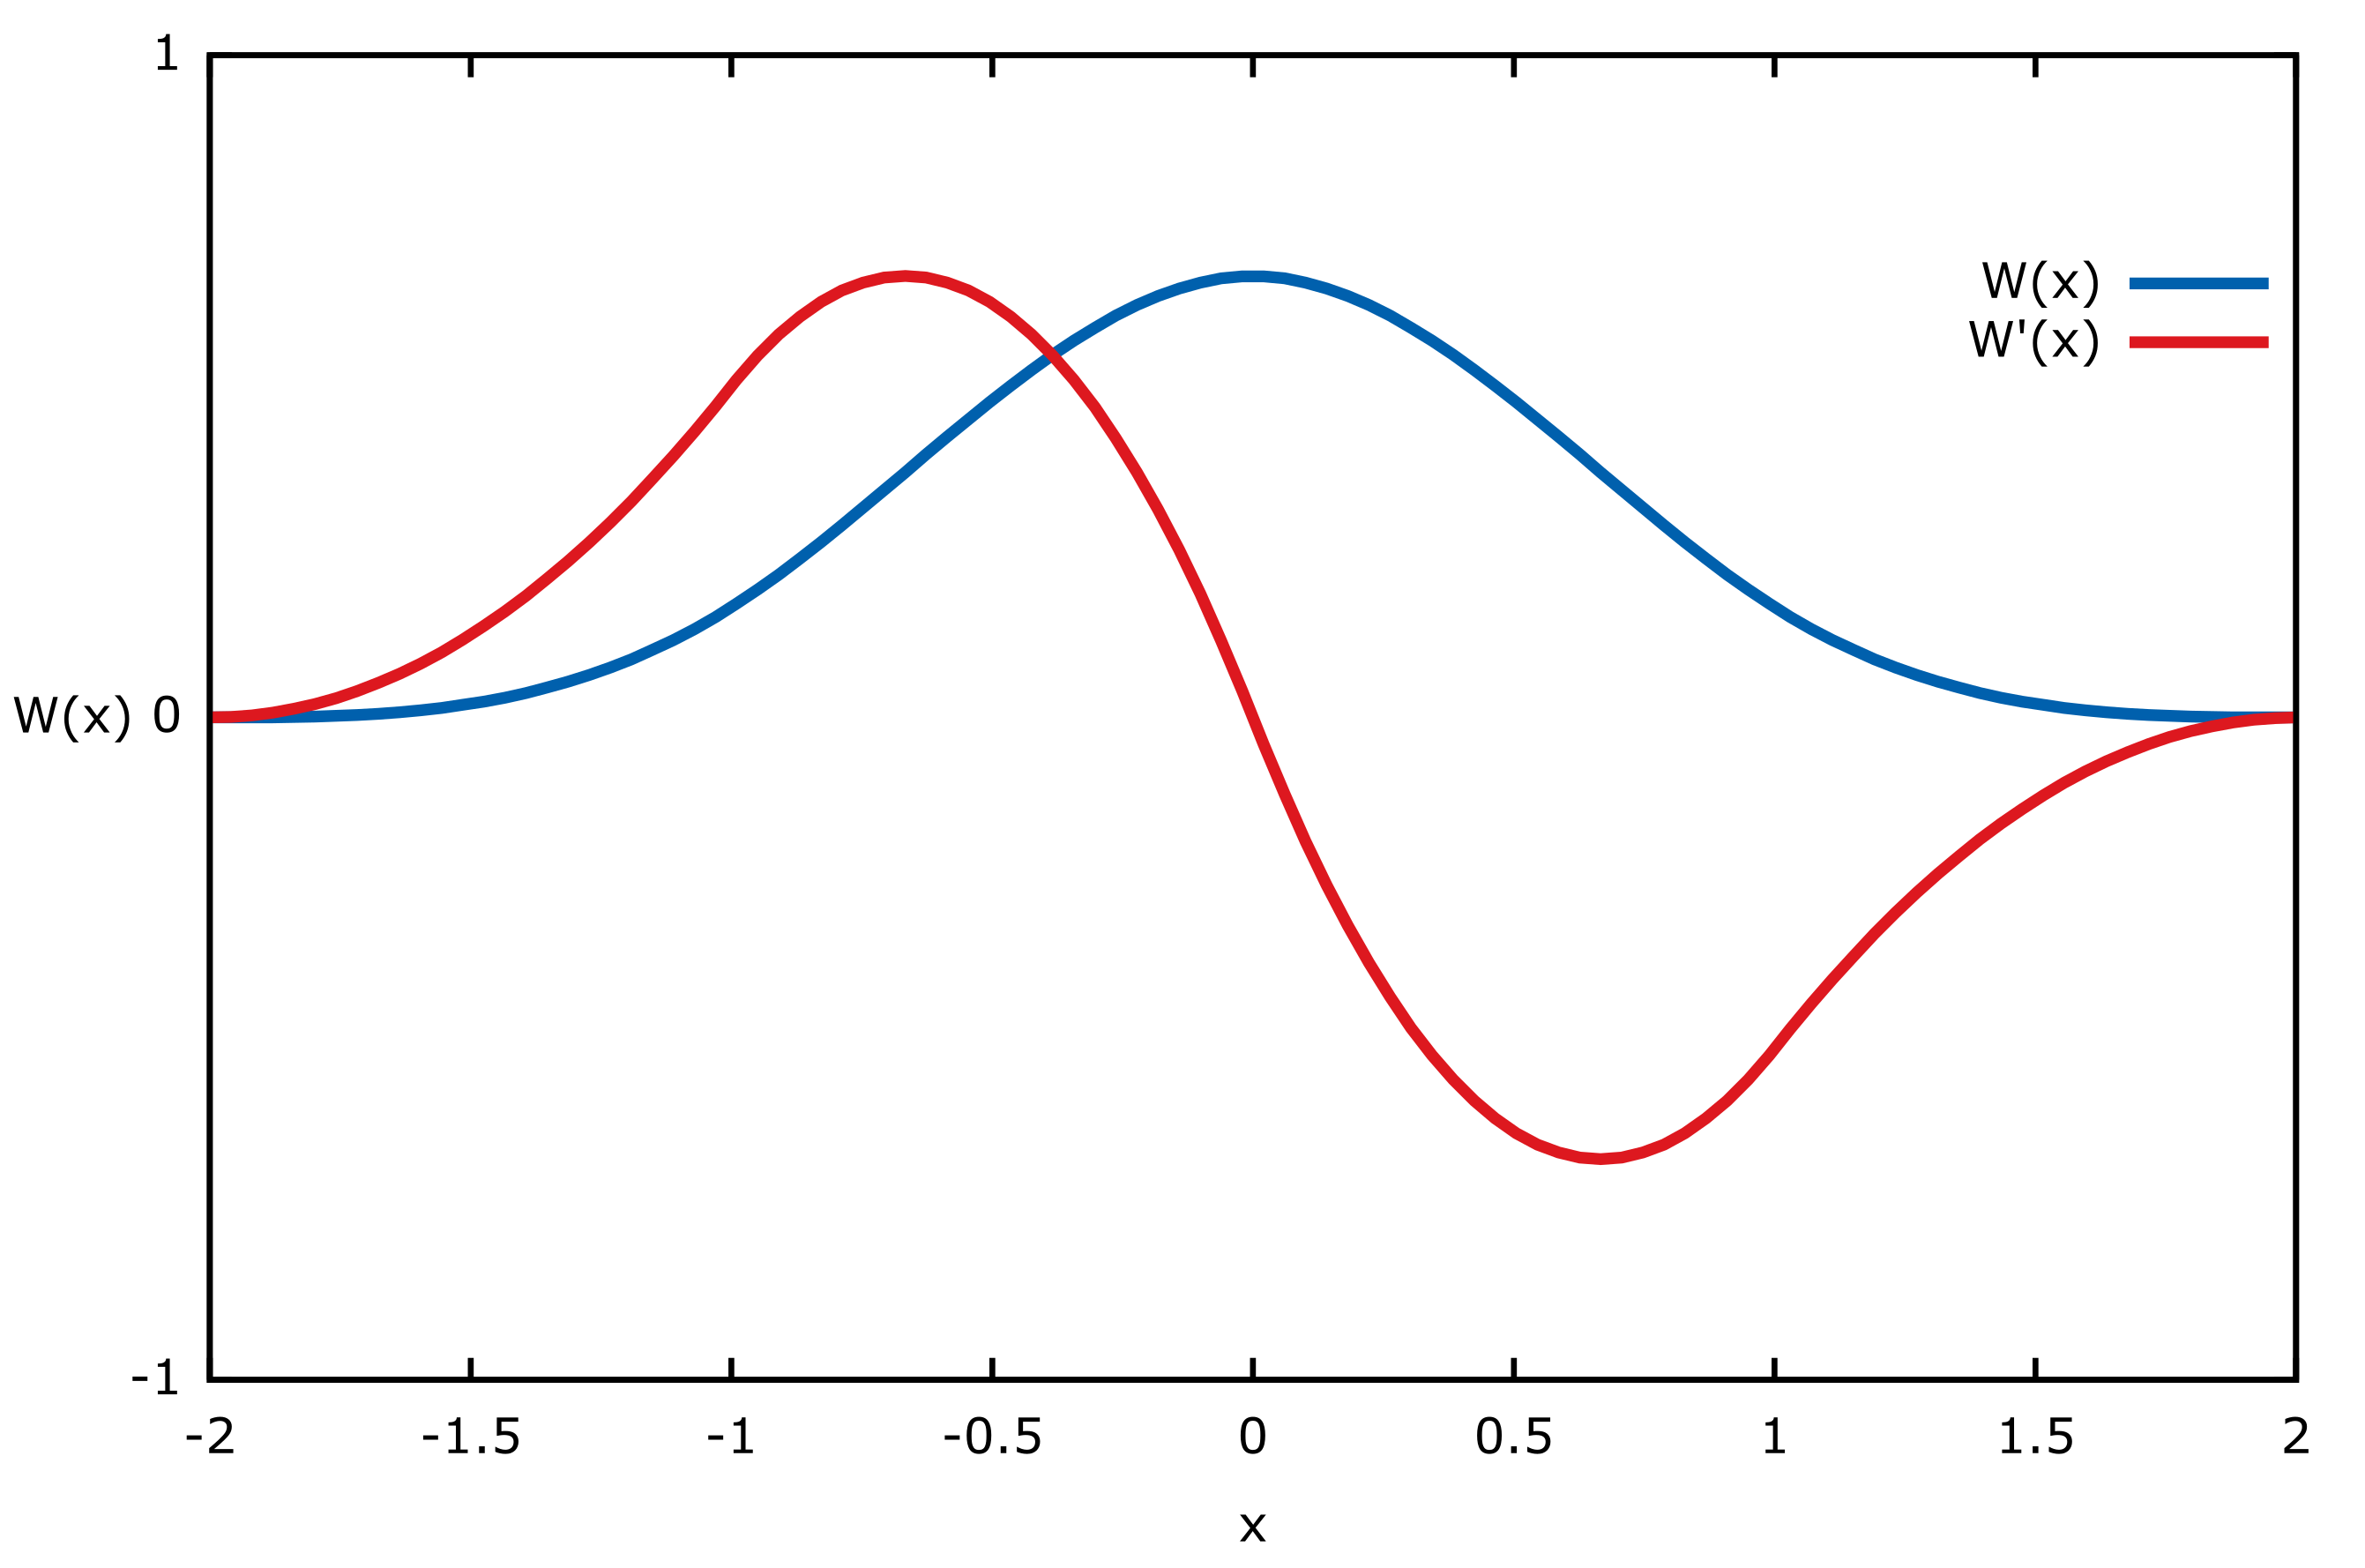
\includegraphics[width=\linewidth]{images/continuum_mechanics/cubicKernel.png}
	\caption[STAR mechanics: Cubic kernel]{\label{fig:cubicKernel}
		Illustration of the 1D cubic kernel used by Monaghan et al.~\cite{Monaghan1992} and its derivative for $h=1$. Note that the support of $W$ is $2h$.}
\end{figure}
This kernel meets properties which are generally required from $W$
\begin{itemize}
\item $W$ is normalized. Thus, constants are interpolated exactly.
\item $W$ has a compact support.
\begin{equation}
\parallel \mathbf{x} \parallel \geq h \implies W(\mathbf{x},h) = 0 
\end{equation}
\begin{equation}
\int_{\mathcal{V}} W(\mathbf{x},h) dx = 1
\end{equation}
\item $W$ tends to the delta function when the length scale $h$ tends to $0$.
\begin{equation}
\lim_{h \rightarrow 0} W(x,h) = \delta(x)
\end{equation}
\item $W$ should be symmetric to enforce invariance under rotation
\begin{equation}
W(-x,h) = W(x,h)
\end{equation}
\item Depending on the function to interpolate the kernel should be positive to prevent unphysical interpolated value.
\begin{equation}
W \geq 0
\end{equation}
\end{itemize}
Here we can notice a first limitation of SPH: For a constant function $f$, the approximation of its first derivatives using Equation~\eqref{eq:sphFunction} will not necessarily vanish depending on $W$. A common practice to fix that is to consider the derivative of the product of $f$ with an arbitrary differentiable function that we note $\Phi$
\begin{equation}
\label{eq:hackSPH}
\nabla f = \frac{1}{\Phi}\left(\nabla (f \Phi) - f \nabla \Phi \right)
\end{equation}
In this case, we can approximate $\nabla(f\Phi)$ and $\nabla \Phi$ using Equation~\eqref{eq:sphFunction}. If $f$ is constant, we will get $\nabla f = 0$. In practice the density $\rho$ is often used for $\Phi$. In the following paragraph, we will see another usage of this technique.
\paragraph{Application to Navier-Stokes equations}
First of all, let us discretize Navier-Stokes equation on the sampling of the particles using the midpoint rule:
\begin{equation}
\label{eq:particleNavierStokes}
\left\lbrace
\begin{array}{ll}
\displaystyle \sum_{i=0}^{N} \left( \rho_{i} \frac{d}{dt} \mathbf{v}_{i} + \nabla p_{i} - \eta \Delta \mathbf{v}_{i} - \rho_{i} \mathbf{g} \right) V_{i} = \mathbf{0}\\ \\
\displaystyle \sum_{i=0}^{N} \nabla. \mathbf{v}_{i} V_{i} = 0
\end{array}
\right.
\end{equation}
We can omit the mass conservation as we did before, by assuming that the particles have a fixed mass through the simulation. Recently, Bender and Koschier~\cite{Bender2015} demonstrated that this simplification prevents from using larger time steps. But for the sake of simplicity, we will keep this approximation in the remainder of this manuscript. Now, we can discretize each term of the equations for a particle $i$ using the SPH technique from Equation~\eqref{eq:sphFunction}.
\subparagraph{Density}
\begin{equation}
\label{eq:densitySPH}
\rho_{i} = \sum_{j=0}^{N} m_{j}W(\mathbf{x_{i}}-\mathbf{x_{j}},h)
\end{equation}
\subparagraph{Pressure}
\begin{equation}
\label{eq:pressureSPH}
p_{i} = k\left(\rho_{i}-\rho_{0}\right)
\end{equation}
where 
\begin{itemize}
\item $\rho_{0}$ is the rest density of the fluid ($1000\kilo\gram\per\meter\cubed$).
\item $k$ is a stiffness parameter.
\end{itemize}
Equation~\ref{eq:pressureSPH} is a simple and cheap computation of the pressure. This equation of state acts like a spring in order to enforce the incompressibility of the fluid.
However, a high stiffness is generally needed to get close to incompressibility. Therefore, very small time steps are required to ensure stability. Recently, new techniques were proposed to ensure incompressibility while using larger time steps. We do not detail these methods in this manuscript but refer the reader to the work of Ihmsen et al.~\cite{Ihmsen2014:IISPH} and Bender and Koschier~\cite{Bender2015}.
\subparagraph{Pressure gradient}
\begin{equation}
\left(\nabla p\right)_{i} = \sum_{j=0}^{N} \frac{m_{j}}{\rho_{j}} p_{j} \nabla W(\mathbf{x_{i}}-\mathbf{x_{j}},h)
\end{equation}
Here we can notice that the resulting pressure force between two particles $i$ and $j$ is not symmetric and therefore does not conserve linear and angular momentum:
\begin{equation}
\label{eq:nonSymmetricPressureForce}
\mathbf{f}^{pressure}_{ij} = -\frac{m_{i}m_{j}}{\rho_{i}\rho_{j}}p_{j}\nabla W(\mathbf{x_{i}}-\mathbf{x_{j}},h)
\end{equation}
To remedy this problem, we can use Equation~\eqref{eq:hackSPH} with $\displaystyle \Phi = \frac{1}{\rho_{i}}$
\begin{equation}
\left(\nabla p\right)_{i} = \rho_{i} \left( \nabla \left(\frac{p_{i}}{\rho_{i}}\right) + p_{i}\frac{\nabla \rho_{i}}{\rho_{i}^{2}}\right)
\end{equation}
and re-use SPH interpolation to get a new approximation of the pressure gradient
\begin{equation}
\label{eq:pressureGradientSPH}
\left(\nabla p\right)_{i} = 
\rho_{i}
\sum_{j=0}^{N} m_{j} \left( \frac{p_{i}}{\rho_{i}^{2}} + \frac{p_{j}}{\rho_{j}^{2}} \right) \nabla W(\mathbf{x_{i}}-\mathbf{x_{j}},h)
\end{equation}
which results into symmetric pressure forces between two particles $i$ and $j$:
\begin{equation}
\label{eq:symmetricPressureForce}
\mathbf{f}^{pressure}_{ij} = m_{i}m_{j}
-\left( 
\frac{p_{i}}{\rho_{i}^{2}} + \frac{p_{j}}{\rho_{j}^{2}} 
\right) 
\nabla W(\mathbf{x_{i}}-\mathbf{x_{j}},h)
\end{equation}
\subparagraph{Velocity Laplacian}
\begin{equation}
\left(\Delta \mathbf{v}\right)_{i} = \sum_{j=0}^{N} \frac{m_{j}}{\rho_{j}} \mathbf{v}_{j} \Delta W(\mathbf{x_{i}}-\mathbf{x_{j}},h)
\end{equation}
Same as for the pressure gradient, this would result in a non-symmetric inter-particle viscosity force:
\begin{equation}
\label{eq:nonSymmetricViscosityForce}
\mathbf{f}^{viscosity}_{ij} = \eta\frac{m_{i}m_{j}}{\rho_{i}\rho_{j}}\mathbf{v}_{j}\Delta W(\mathbf{x_{i}}-\mathbf{x_{j}},h)
\end{equation}
If we assume that the density is constant, which is the case in theory, we could obtain symmetric forces by using Equation~\eqref{eq:hackSPH} with $\Phi=\rho_{i}$. However, in practice, the density is not constant and the evaluation of the Laplacian of the kernel is sensitive to particles sampling, which makes this solution inadequate.
Actually, it is quite hard to correctly handle viscosity using SPH and this is still an area of research, especially for liquids exhibiting complex viscous behaviors such as coiling or buckling.
We refer the reader to the recent work of Peer et al.~\cite{Peer2015} and Takahashi et al.~\cite{Takahashi2015} about this topic.
For fluid with a low viscosity, Monaghan~\cite{Monaghan2005} proposed a gradient-based formulation of the Laplacian which results in symmetric forces,
\begin{equation}
\label{eq:velocityLaplacianSPH}
\left(\Delta \mathbf{v}\right)_{i} = 
\frac{1}{\rho_{i}}
\sum_{j=0}^{N} m_{j} \Pi_{ij} \nabla W(\mathbf{x_{i}}-\mathbf{x_{j}},h)
\end{equation}
where 
\begin{equation}
    \Pi_{ij} = -\frac{2hc_{s}}{\rho_{i}+\rho_{j}}\frac{\mathbf{v}_{ij}^{T}\mathbf{x}_{ij}}{\vert \mathbf{x}_{ij} \vert^{2} + \epsilon h^{2}}
\end{equation}
and $c_{s}$ is the speed of sound in the media and $\epsilon$ is a numerical constant to avoid singularities.
In practice, $\epsilon=0.01$ works well. We will use this formulation in Section~\ref{sec:arps_sph}.
\subparagraph{Time integration} If we assume a uniform discretization of the time based on a time step $\Delta t$, symplectic Euler is common choice to integrate the equations of motion over time and for a particle $i$ we get
\begin{equation}
\begin{array}{ll}
\displaystyle \mathbf{v}_{i}(t+\Delta t) = \mathbf{v}_{i}(t) + \frac{\Delta t}{m_{i}}\left( \sum_{j=0}^{N}\left(\mathbf{f}_{ij}^{pressure}+\mathbf{f}_{ij}^{viscosity}\right)+m_{i}\mathbf{g}\right) \\ \\
\displaystyle \mathbf{x}_{i}(t+\Delta t) = \mathbf{x}_{i}(t) + \Delta t \mathbf{v}_{i}(t+\Delta t)
\right.
\end{equation}
We described the key ingredients of the SPH model and how to use them to discretize Navier-Stokes equations. 
There is not enough space to cover the exciting challenges related to the building of a full SPH simulator. 
For a robust handling of static and dynamic boundaries, a surface tension model and an efficient surface reconstruction pipeline, we refer to the work of Akinci et al.~\cite{Akinci2012b, Akinci2013, Akinci2012a}.  
For a state of the art of optimization techniques for SPH, we refer the reader to the work of Ihmsen et al.~\cite{Ihmsen2011:ParallelSPH}. 
For other references related to the handling of viscosity, multiphase simulations and other problems, the state of the art report on SPH by Ihmsen et al.~\cite{Ihmsen2014:STAR} is a safe starting point.

\subsection{Solid mechanics}
\label{subsec:solidMechanics}

\begin{figure}[!ht]
\centering
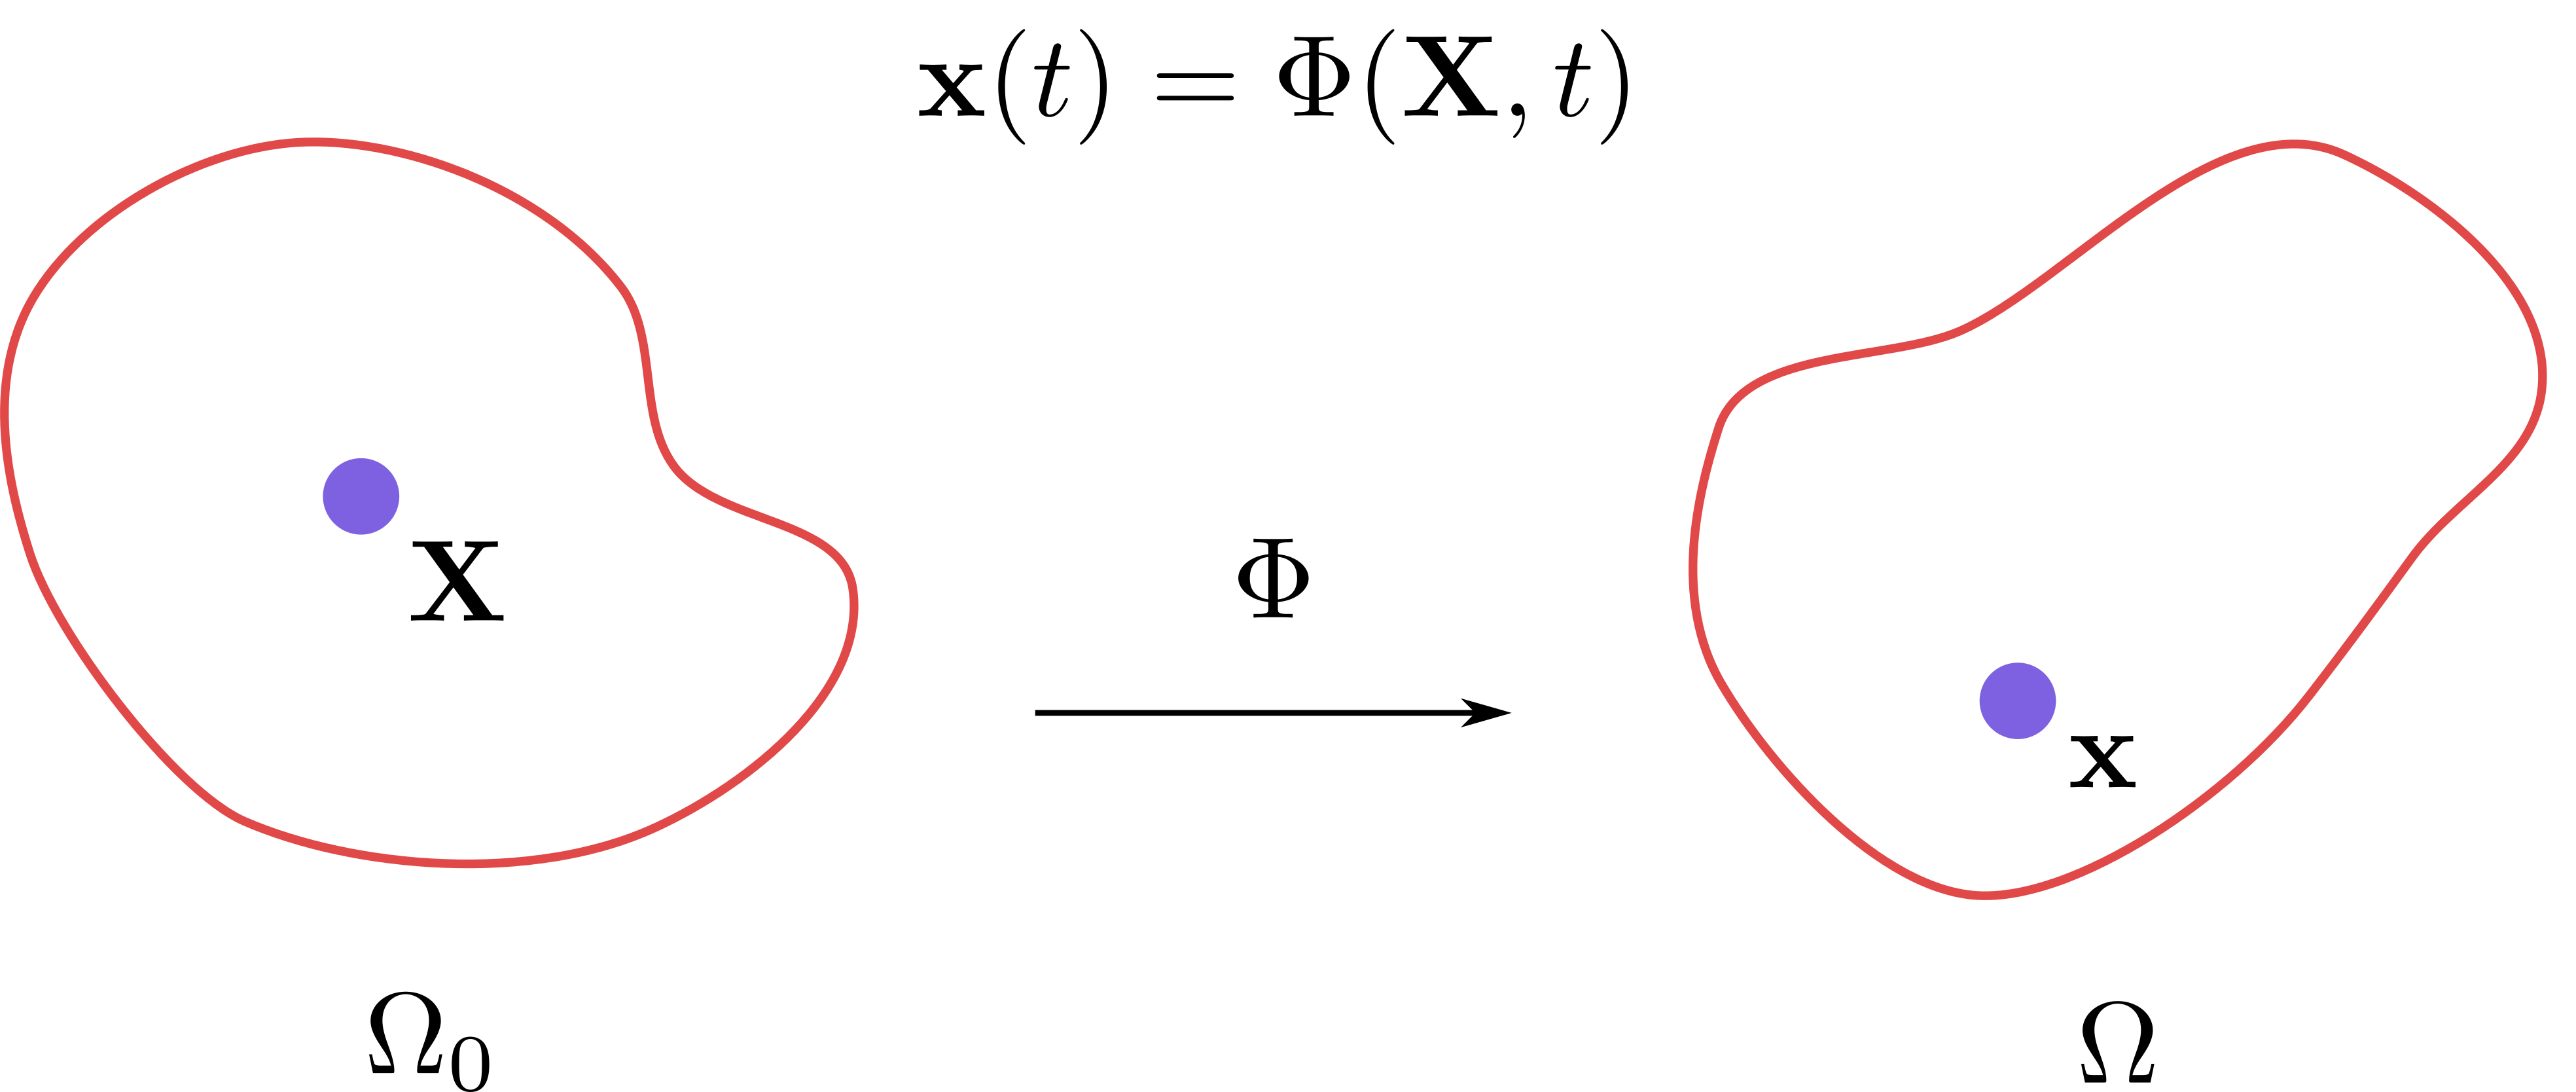
\includegraphics[scale=0.4]{./images/continuum_mechanics/displacementField.png}
\caption[STAR mechanics: Displacement field]{\label{fig:displacementField}
 The displacement field $\Phi$ maps each point $\mathbf{X}$ from the rest configuration $\Omega_{0}$ to a point $\mathbf{x}$ in the deformed configuration $\Omega$.}
\end{figure}

In this section, we focus on the simulation of elastic objects. When submitted to external forces, an elastic object reacts so that it comes back to its rest shape. In contrast with fluids, internal forces are history dependent, they depend on how much the object deformed compared to its rest shape. It becomes crucial to be able to describe the deformation of an object in order to express its reaction. 

The deformation is modeled by a mapping $\Phi$ between the undeformed configuration $\Omega_{0}$ and the deformed configuration $\Omega$ (see Figure~\ref{fig:displacementField}). $\Phi$ is called the \emph{displacement field}.
\begin{equation}
\begin{array}{lllll}
\Phi & : & \Omega_{0} & \longrightarrow & \Omega \\
	 &  & \mathbf{X} & \longrightarrow & \mathbf{x}
\end{array}
\end{equation}
where $\mathbf{X}$ is a point in the undeformed configuration and $\mathbf{x}=\Phi(\mathbf{X})$ is the mapped point into the deformed configuration.

The deformation gradient $\displaystyle F = \frac{\partial \Phi}{\partial \mathbf{X}}$ describes the local state subject to rigid and/or deformable displacement with respect to the undeformed configuration. 
The strain tensor $\epsilon$ measures the deformation.
Multiple strain measures have been proposed, Green-Lagrange strain can be used for instance: $\displaystyle \epsilon = \frac{1}{2}\left(F^{T}F - I\right)$. 
Or its linearized version, the Cauchy strain $\displaystyle \epsilon = \frac{1}{2}\left( F + F^{T} \right)-I$.

The displacement field, deformation gradient and strain tensor are the main components of the constitutive law that relates the deformation to the material properties of the object.

\subsubsection{Constitutive Law}
In this section, we focus on elastic materials, i.e objects which tends to recover their rest configuration after a deformation.
For elastic materials, the stress tensor $\sigma$ can be described using constitutive density energy $\Psi$ that is derived with respect to the strain tensor $\epsilon$:

\begin{equation}
\label{eq:constitutiveLaw}
\sigma = \frac{\partial \Psi}{\partial \epsilon}
\end{equation}

Different forms of energy exist. For a classical Hookean material, the density energy is
\begin{equation}
\Psi = \frac{1}{2}H\epsilon^{2}
\end{equation}

which gives the following stress tensor
\begin{equation}
\sigma = H\epsilon
\end{equation}

$H$ is called the stiffness tensor and is a $3\times3\times3\times3$ tensor. 
For isotropic materials, the number of material parameters can be reduced to two, the Young's modulus $E$ and the Poisson's ratio $\nu$. 
These parameters respectively describes the resistance of the object to extension and to shearing.
Moreover, the strain and stress tensor are symmetric which allows to simplify the constitutive law:
\begin{equation}
\sigma = 
\begin{bmatrix}
\sigma_{11} \\
\sigma_{22} \\
\sigma_{33} \\
\sigma_{23} \\
\sigma_{13} \\
\sigma_{12}
\end{bmatrix}
=
\tilde{H}
\begin{bmatrix}
\epsilon_{11} \\
\epsilon_{22} \\
\epsilon_{33} \\
2\epsilon_{23} \\
2\epsilon_{13} \\
2\epsilon_{12}
\end{bmatrix}
\end{equation}

where

\begin{equation}
\tilde{H} =
\frac{E}{\left(1+\nu\right)\left(1-2\nu\right)}
\begin{bmatrix}
1-\nu & \nu & \nu & 0 & 0 & 0 \\ 
\nu & 1-\nu & \nu & 0 & 0 & 0 \\
\nu & \nu & 1-\nu & 0 & 0 & 0 \\
0 & 0 & 0 & \frac{1-2\nu}{2} & 0 & 0 \\
0 & 0 & 0 & 0 & \frac{1-2\nu}{2} & 0 \\
0 & 0 & 0 & 0 & 0 & \frac{1-2\nu}{2} \\
\end{bmatrix}
\end{equation}

Instead of computing internal forces as the divergence of the stress, they can be computed as the derivative of the density energy with respect to the degrees of freedom:
\begin{equation}
\label{eq:internalForces_solids}
\mathbf{f} = -\int_{\mathcal{V}} \frac{\partial \Psi}{\partial \mathbf{x}}^{T} dv
\end{equation}

\subsubsection{Frame-based model}
\label{subsubsec:framebased}
The frame-based model was introduced by Gilles et al.~\cite{Gilles2011} to simulate deformable objects. In contrast to other deformable models, it allows to simulate complex object with very few degrees of freedom and to handle heterogeneous materials easily \cite{Faure2011}. 
Additionally, this work formalized the concept of multi-layer physical framework. In the following, we first describe what is a multi-layer framework, illustrate it in the case of the frame-based model. 
Then we detail a standard choice for the different components of the frame-based model: degrees of freedom, interpolation and integration. As in the previous section, this section is a high level overview. 
Detailing collision detection and response processes and giving a more accurate formulation of viscosity via the strain rate are out of the scope of this chapter.

\paragraph{A multi-layer physical framework}
 
\begin{figure}[!ht]
\centering
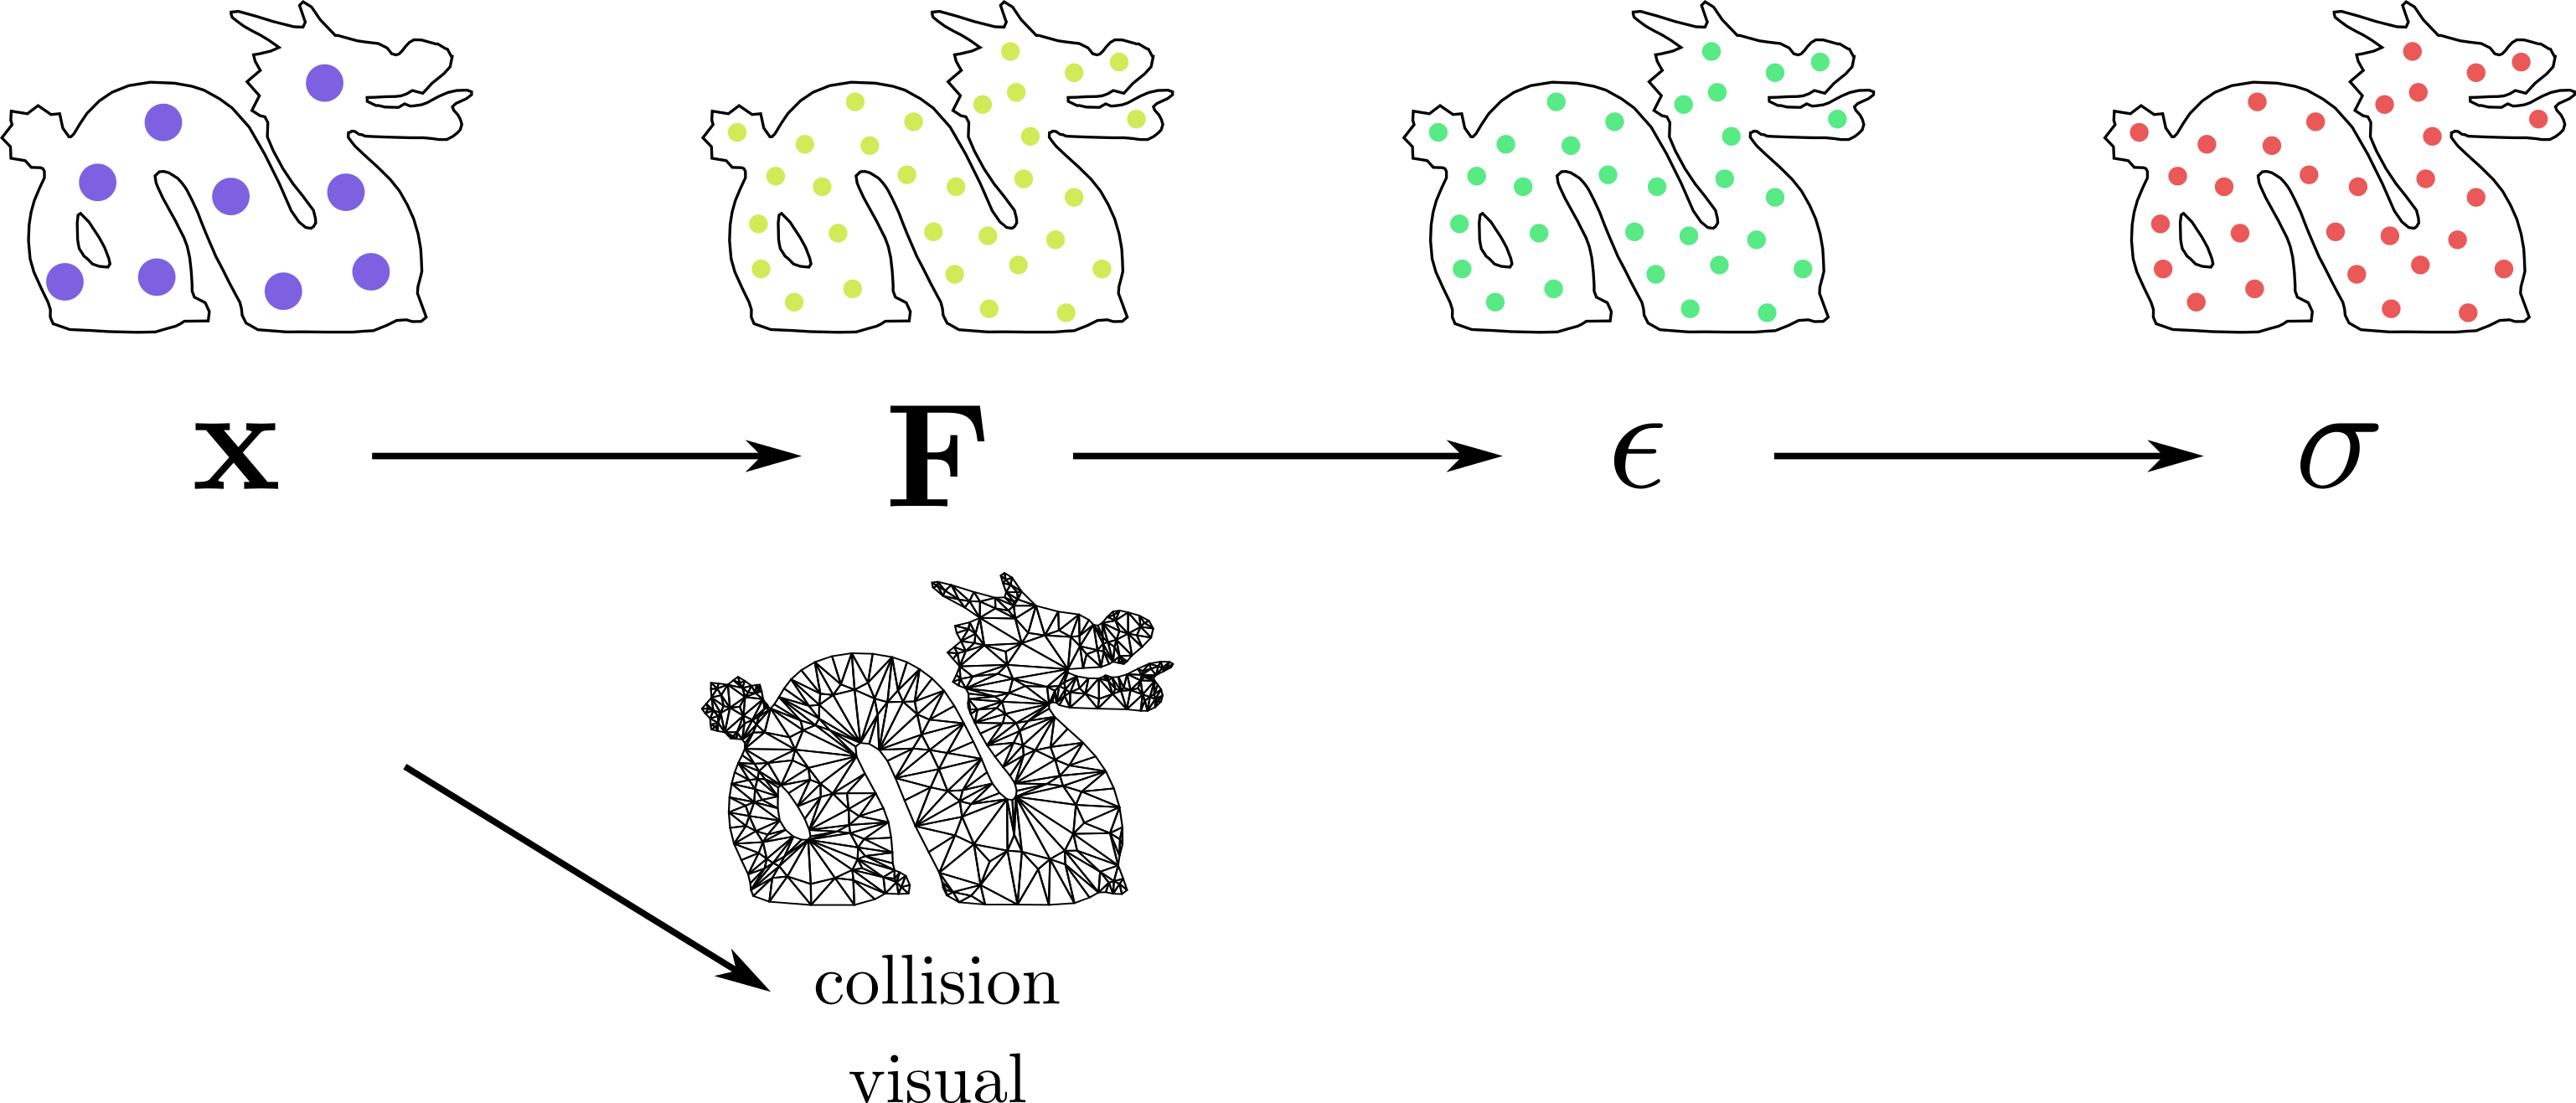
\includegraphics[width=\linewidth]{./images/continuum_mechanics/multiLayeredFramework.png}
\caption[STAR mechanics: Multi-layer framework]{\label{fig:multiLayerFramework} Each component of the simulation is isolated and communicates with other components through mappings. By doing so, the framework allows fast prototyping and comparison of a wide range of deformable models.}
\end{figure}

Most of the time, the different components of a physics-based model are described as a monolithic framework: degrees of freedom, interpolation, integration and constitutive law are put together in one formula which computes the forces applied on the degrees of freedom. On one hand, this provides a compact and implementation-friendly expression. It also suits the short format of scientific article. On the other hand, it requires assumptions on each component and make it hard to distinguish what should be changed in order to integrate collisions, to embed a visual model or to test variations of the initial model.

An interesting alternative is to build a multi-layer framework where each component of a physics-based model represents a layer which is able to communicate with other layers through mappings. 
The framework has then a great modularity, as different components can be re-used and mixed. A direct consequence is the ease at prototyping. 
State of the art methods can be implemented in hours instead of days. 
Comparisons of different models is much easier. 
Also, it provides a way to control the granularity of a simulation, as each layer can be discretized at its own resolution, this allows for an easier repartition of resources and computational tasks.

In their work, Gilles et al. \cite{Gilles2011} proposed such an alternative by decomposing the computation of force using the derivation chain rule:
\begin{equation}
\label{eq:forceChainRule}
\displaystyle \mathbf{f} = -\int_{V} \left(\frac{\partial \Psi}{\partial \mathbf{x}}\right)^{T} dv
=
-\int_{V} \left(\frac{\partial F}{\partial \mathbf{x}}\right)^{T}
\left(\frac{\partial \epsilon}{\partial F}\right)^{T}
\left(\frac{\partial \Psi}{\partial \epsilon}\right)^{T} dv
\end{equation}
The three different layers are now visible: the degrees of freedom, the deformation gradient, the strain tensor and the constitutive density energy.
Moreover, we can distinguish the Jacobian of the mappings that link degrees of freedom to deformation gradient and deformation gradient to strain.
Notice that the derivative of the constitutive density energy with respect to strain is actually the stress tensor presented in Equation~\eqref{eq:constitutiveLaw}.

Using this modular representation offers three main advantages: 
First, layers and mappings can be implemented separately thus providing a great deal of modularity;
Secondly, it is straightforward to have a sampling of degrees of freedom different from the sampling of integration points.
Thus, multi-resolution strategies can easily be integrated. 
For instance, we might want a small number of degrees of freedom to have a small computational time during the solving of dynamics while computing accurate deformation gradient, strain and stress which requires a dense sampling of integration points.
Additionally, embedding techniques, used to display a fine visual model or to handles collision with a coarse representation, fits well in this framework.

In the case of the frame-based method, there are two additional layers, one for embedding a visual model and one for handling collisions. 
Both communicate with the degrees of freedom through a mapping which is the displacement field (see Figure~\ref{fig:multiLayerFramework}).

\paragraph{Degrees of freedom}
The object is uniformly sampled with affine frames as degrees of freedom. An affine frame $T=(A,\mathbf{t})$ represents $12$ degree of freedoms, $3$ for translation $\mathbf{t}$, $9$ for the matrix $A$ combining rotation, scaling and shearing. 
Affine frames are expressed with respect to an initial configuration ~$T_{0} = \left(A_{0}, \mathbf{t}_{0}\right)$.

\paragraph{Interpolation}
Linear blend skinning is used to interpolate the displacement field and other quantities of the simulation. A deformed position $\mathbf{x}$ can be interpolated as a weighted sum of the affine transformations applied to the rest position $\mathbf{x}_{0}$.

\begin{equation}
\label{eq:frameBasedDisplacementField}
\begin{array}{l}
\displaystyle \mathbf{x} = \Phi(\mathbf{x}_{0}) = \sum_{i} w_{i}(\mathbf{x}_{0})\left(\mathbf{t}_{i}+A_{i}\mathbf{x}_{0}^{rel}\right) \\
\displaystyle \mathbf{x}_{0}^{rel} = A_{0}^{-1}\left( \mathbf{x}_{0} - \mathbf{t}_{0} \right)
\end{array}
\end{equation}

where $\mathbf{x}_{0}^{rel}$ is the relative position of $x_{0}$ in the frame defined by $T_{0}$ and $w_{i}$ is the shape function associated to the frame $i$.

Different weights can be used. Three properties are important in order to represent a physical behavior. 
First, the shape function should linearly decrease with respect to distance in the material. 
Otherwise, the deformation will not be uniform with respect to the distance from the frame. 
Second, the shape function should be positive. 
Third, the weights should form a partition of unity. 
In practice, one can use either harmonic weights or Voronoi-based weights.
In Chapter~\ref{chap:cutting}), we will detail the computation of Voronoi-based weights and how to dynamically update them to take into account topological changes.

From the description of the displacement field (Equation~\eqref{eq:frameBasedDisplacementField}), the deformation gradient can then be derived:
\begin{equation}
\displaystyle
F\left(\mathbf{x}\right) = \sum_{i} \frac{\partial \mathbf{x}}{\partial \mathbf{x}_{0}} =
\nabla w_{i}(\mathbf{x}_{0}) \left( \mathbf{t}_{i}+A_{i}\mathbf{x}_{0}^{rel}\right) + 
w_{i}\left( A_{i}A_{0}^{-1} \right)
\end{equation}

\paragraph{Spatial integration}

Any quadrature rule can be used. Here, for the sake of simplicity, we suppose that we use the midpoint rule briefly described in Figure~\ref{fig:spatialIntegration}. Thus, the integral of a function $f$ over the object states:
\begin{equation}
\displaystyle
\int_{V} f(\mathbf{x})  = \sum_{p} V_{p} f(\mathbf{x}_{p})
\end{equation}
where $p$ is an integration point and $V_{p}$ its associated volume.
\\ \\
From this quadrature rule, we can now formulate the computation of internal forces for one frame as:
\begin{equation}
\label{eq:frameForceComputation}
\displaystyle
\mathbf{f}_{i} =
- \sum_{p}
\left( \frac{\partial F}{\partial \mathbf{x}_{i}} \right)^{T}
\left( \frac{\partial \epsilon}{\partial F} \right)^{T}
\left( \frac{\partial \Psi}{\partial \mathbf{\epsilon}} \right)^{T} \left(\mathbf{x_{p}}\right) V_{p} 
\end{equation}
where $p$ is an integration point, $\mathbf{x}_{p}$ its position and $V_{p}$ its associated volume.

\paragraph{Temporal integration}

Assuming the mass matrix is lumped and that we use explicit Euler, the time integration of one frame $i$ is:
\begin{equation}
\displaystyle
\begin{pmatrix}
\mathbf{t}_{i}(t+\Delta t) \\
A_{i}(t+\Delta t)
\end{pmatrix} 
=
\begin{pmatrix}
\mathbf{t}_{i}(t) \\
A_{i}(t)
\end{pmatrix} 
+
\Delta t
M_{i}^{-1}
\mathbf{f}(t)
\end{equation}
where $M_{i}$ is the mass matrix of the frame $i$:
\begin{equation}
\label{eq:massMatrix}
M_{i} = \int_{V} w_{i}^{T} \rho w_{i} dv
\end{equation}
and $w_{i}$ is the shape function of the frame $i$.

\subsection{Conclusion on continuum mechanics}

In this section, we briefly presented the basics of continuum mechanics.
First, we described how to design equations of motion and which numerical tools are involved in their solving. 
Then, for fluids and solids mechanics, we mentioned their specificities and detailed a deformable model.
We illustrated the fact that continuum mechanics allows to automatically compute realistic motion from a wide range of phenomena.
This strength mainly explains why hand-made animations of physical phenomena have been replaced by physics-based animation.
However, realism comes with a high computational cost.
This cost may make large scale simulations intractable or prevent from simulating advanced phenomena in interactive context.
In the following section, we review adaptive models, a common approach to make simulations efficient.

%\section[Adaptive physics-based animation]{Adaptive techniques and models for physics-based animation}
\label{sec:starAdaptivity}
Complex real-world behaviors may exhibit multi-scale phenomena in space and time, large deformations or topological changes.
Sophisticated physical models involving a tremendous number of degrees of freedom are required to accurately reproduce these phenomena.
This comes at a high memory and computational price that can quickly become intractable or prevent from an interactive usage.
Adaptive models provide a general paradigm to solve these efficiency goals.

We call a model or simulation method \emph{adaptive} if it automatically adapts the underlying mathematical representation, data structure and/or algorithm at run time, based on the evolving state of the simulated system.
The adaptation is designed for meeting a given criteria which depends on the application. 
Examples of frequently used criteria include reducing the overall computational complexity without loss of quality, improving the quality of real-time simulation, or simulating more precisely the parts of the scene with which the user is currently interacting.

In this section, we review the different families of adaptive methods and present the way they have been applied in the different domains. In Section~\ref{sec t adaptivity}, we present time adaptive techniques such as dynamic time stepping and freezing techniques.
Then, we focus on spatially adaptive techniques.
Section~\ref{sec:spatial_refinement} discusses the most popular approach of spatial adaptivity: geometric adaptivity(\textit{h}-adaptivity where \textit{h} classically refers to the size of elements in the finite element method), which refers to varying the discretization resolution via refinement and coarsening strategies. This section is subdivided according to the types of adaptive spatial discretization.
Section~\ref{sec pr adaptivity} covers other spatial adaptivity approaches: basis refinement which adapts the number of bases, their order (\textit{p}-adaptivity where \textit{p} stands for polynomial), the basis functions themselves using enrichment, or, in subspace simulation, the deformation modes of the basis; moving grids methods (\textit{r}-adaptivity where \textit{r} stands for relocation) which relocate nodes without changing their connectivity; and mixed models which selectively apply a combination of different computational models. This organization reflects the taxonomy we propose in Figure~\ref{fig:taxonomy}.
We finally conclude and sketch future research avenues in adaptive simulation.
\paragraph*{}
This section was published in journal \emph{Computer Graphics Forum, 2016}~\cite{Manteaux2016}.
\begin{figure}[!h]
	\centering
	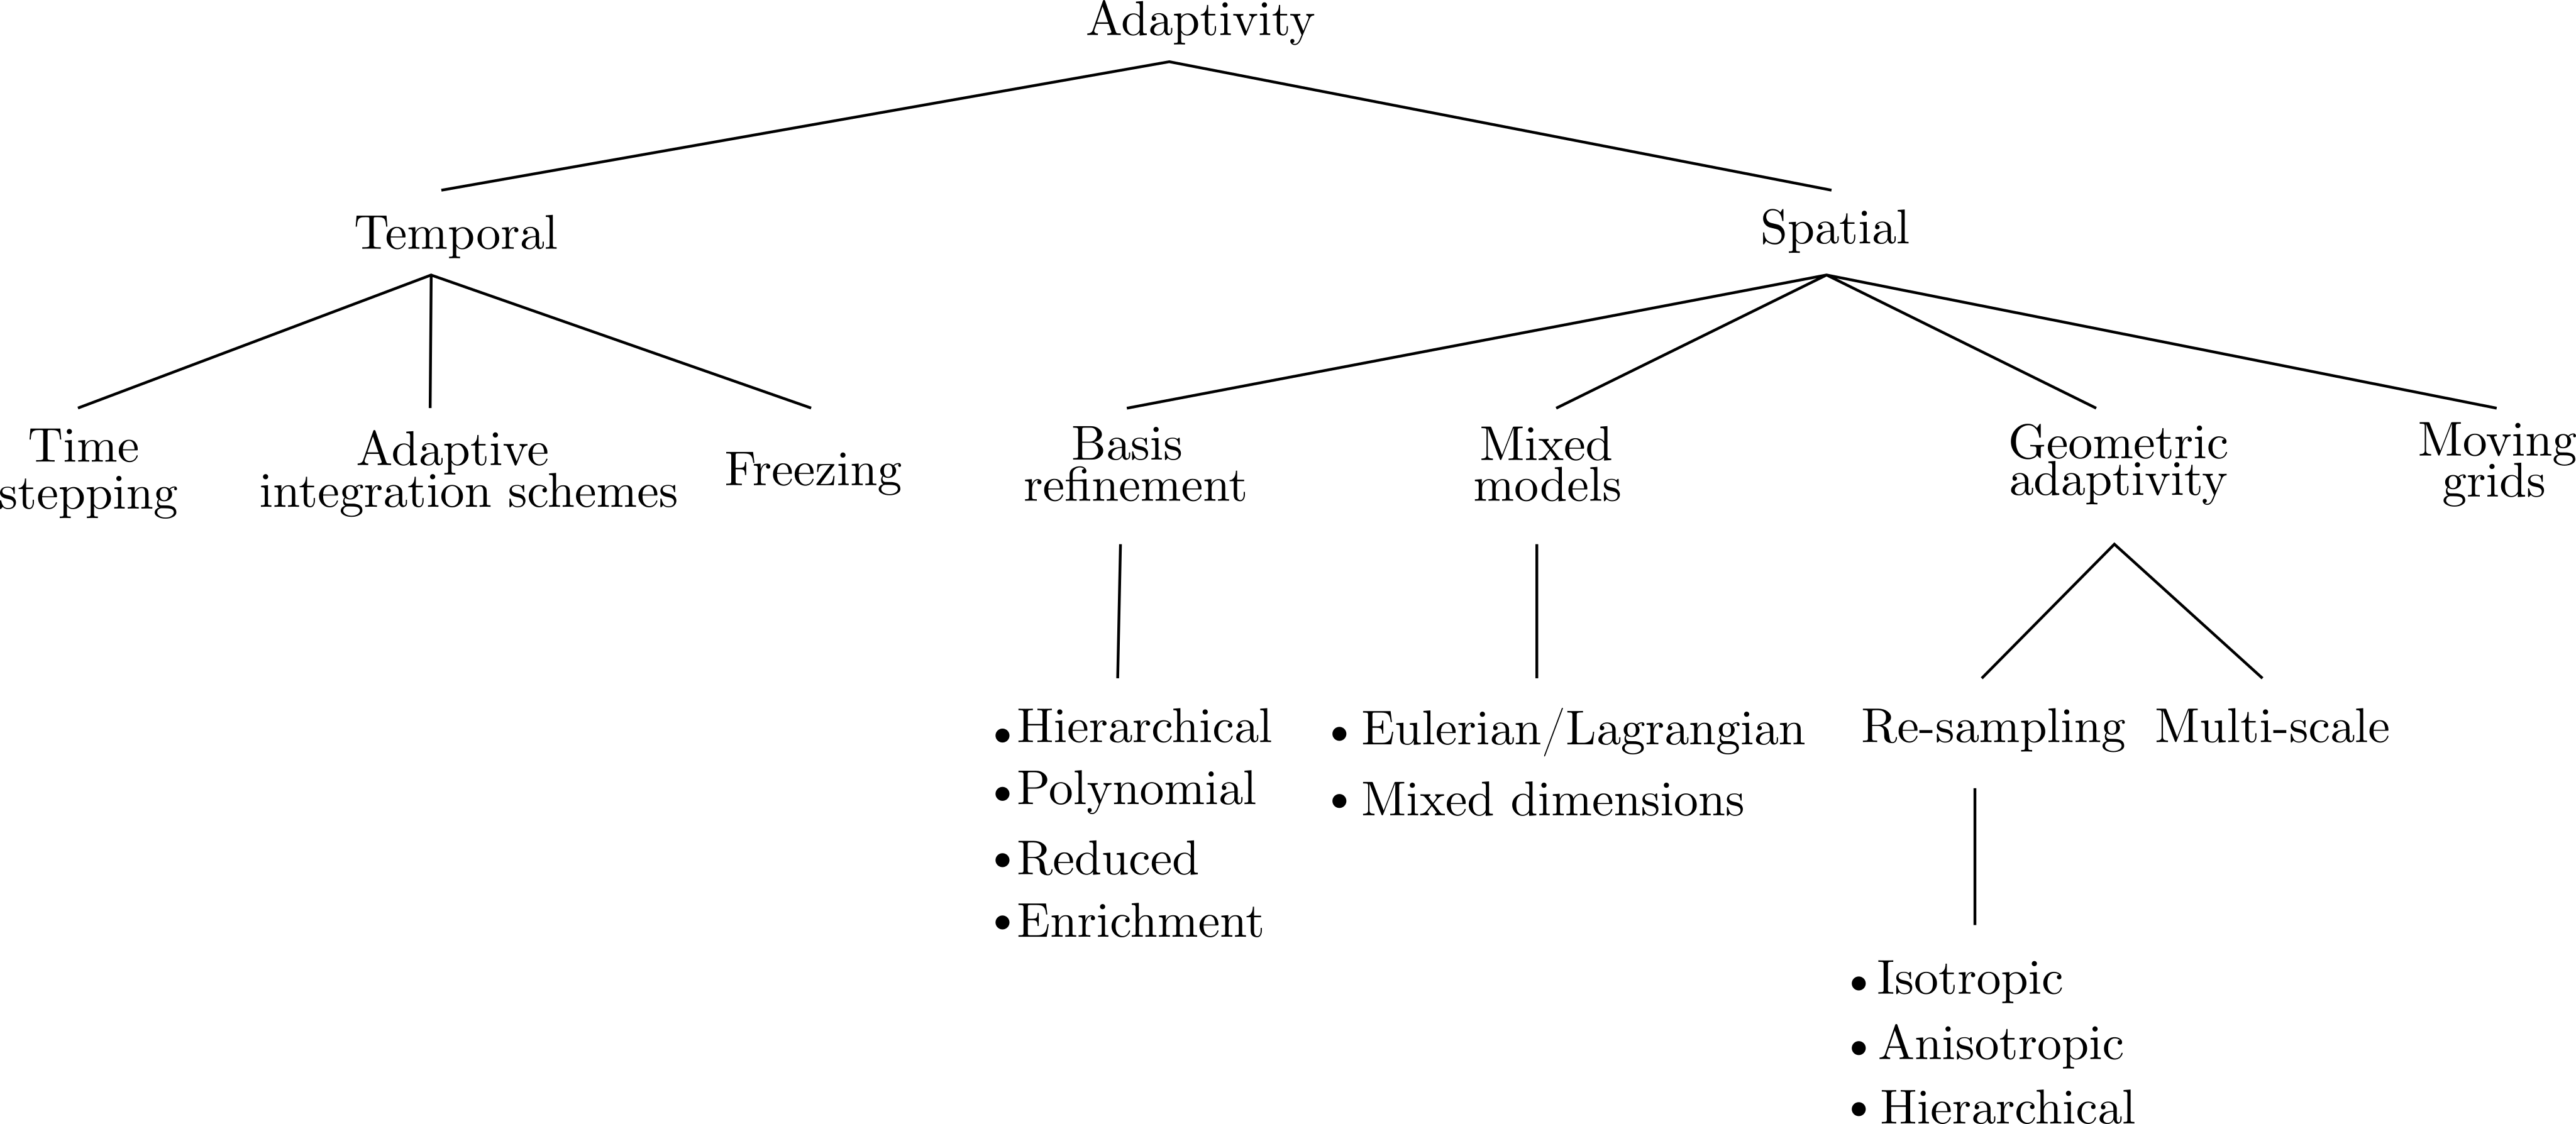
\includegraphics[width=\linewidth]{images/starAdaptivity-cgf2016/taxonomy.png}
	\caption[STAR adaptivity: Taxonomy]{\label{fig:taxonomy}Taxonomy of adaptive physically-based models in Computer Graphics. Temporal adaptivity (see Section \ref{sec t adaptivity}) and geometric adaptivity (see Section~\ref{sec:spatial_refinement}) are the two most common strategies. Basis refinement (see Section~\ref{sec:basis_refinement}), moving grids (see Section~\ref{sec:movingMesh}) and mixed models (see Section~\ref{sec:mixed-models}) are less common but proved to be very promising.}
\end{figure}

\subsection{Temporal adaptivity} \label{sec t adaptivity}
Animating any simulated object requires integrating its equations of motion over time.
There are many reasons why this integration procedure may need to adapt to the circumstances of the simulation, whether for accuracy, consistency, or stability.
For instance, a system entering a highly nonlinear regime, such as during fracture, typically requires smaller time steps to maintain the desired degree of accuracy.
Alternatively, adaptive time steps may be necessary to prevent the system from entering an invalid state: for example, many collision resolution schemes maintain the invariant that the system is never allowed to enter an interpenetrating configuration, which can require adjusting the time step according to the frequency of collisions.
Finally, the stability of continuum-mechanical simulations is closely tied to the relationship between the time step length, the spatial resolution, and the speed of propagation of information in the system, so if either of the latter change (in the presence of \emph{spatial} adaptivity or fast-moving flow) the time step must be adapted as well.
\paragraph*{}
Techniques for temporal adaptivity fall into two main categories.
One approach focuses on time resolution, that is, how to choose an appropriate step length for time integration.
The second focuses on integration techniques themselves, seeking to switch between different integration schemes depending on the local context. This section explores both of these possibilities for temporal adaptivity.

\subsubsection{Adaptive time step selection}

\paragraph*{Time step criteria}
First, let us focus on the simulation of continuous media, like fluids and elastic solids, whose models are governed largely by hyperbolic partial differential equations.
Here the most prominent criterion for time step selection is the Courant-Friedrichs-Lewy (CFL) condition \cite{Courant1928}.
To understand this condition, we first note that the solution of a partial differential equation at some point depends on a particular subset of initial or boundary data; we call this subset of data the \emph{domain of dependence}.
The CFL condition states simply that for any numerical scheme to converge to the true solution, the domain of dependence of the numerical scheme must, in the limit, contain the true domain of dependence of the underlying differential equation.
(Otherwise, one could perturb the initial data in the region outside the numerical domain of dependence and change the true solution without affecting the computed one.)
The CFL condition can also serve as a stability criterion thanks to the Lax-Richtmeyer equivalence theorem \cite{Lax1956,Strikwerda2004}, which states that a consistent finite difference method for a well-posed initial value problem is convergent if and only if it is stable.
\paragraph*{}
For example, for the classical wave equation $\partial_t^2 f = c^2\nabla^2 f$, the domain of dependence of any point $(\mathbf x, t)$ includes only points $(\mathbf x_0, t_0)$ with $\|\mathbf x-\mathbf x_0\|\le c(t-t_0)$, because information propagates only at the wave speed $c$.
Consequently, the time step $\Delta t$ must be small enough to prevent information from propagating outside the spatial stencil over a single time step.
In particular, for the first-order explicit finite difference scheme applied to the wave equation, where over each time step a grid cell is only affected by adjacent grid cells (separated by $\Delta x$), the CFL condition requires that $c\Delta t \le \Delta x$.

In general, the CFL condition typically takes the form
\begin{align}
  \label{eq:cfl}
  C \equiv \frac{c\Delta t}{\Delta x} \le C_{\max},
\end{align}
where $c$ is the speed of information propagation, and $C_{\max}$ is a method-dependent constant which depends on the size of the finite-difference stencils.
The dimensionless ratio $C$ is known as the CFL number or the Courant number.
Note that implicit methods are not restricted by the CFL condition because the solution at any point at the end of the time step depends on the values at \emph{all} the points at the beginning of the time step, so the numerical domain of dependence is effectively infinite.

The CFL condition can be a useful heuristic even in situations where it does not directly apply.
In computer graphics, semi-Lagrangian advection \cite{Stam1999} has been a popular scheme for solving the advection equation, as it is unconditionally stable and not restricted by the CFL condition \cite{Bridson2008}.
Nevertheless, excessively large time steps can lead to undesirable artifacts such as numerical dissipation and volume loss.
Foster and Fedkiw \cite{Foster2001} advocate limiting the time step size using \eqref{eq:cfl} with $c$ being the maximum of the flow speed $\|\mathbf u\|_\infty$ over the domain, and $C_{\max} = 5$.

In Smoothed-Particle Hydrodynamics (SPH), each particle is affected by other particles within its smoothing radius $h$, analogous to the grid separation $\Delta x$ in finite-difference methods.
Consequently, time step selection criteria based on the CFL condition can be applied.
For pressure waves in compressible SPH, we continue to have
\begin{align}
  \label{eq:cfl_sph}
  \Delta t \le C_{\max}\frac hc,
\end{align}
and values of $C_{\max}$ between $0.25$ and $0.4$ have been used \cite{Monaghan1992,Desbrun1999}.
Fast relative motion of particles, which occurs especially during fluid-fluid or fluid-solid collisions, can also produce artifacts due to interactions not considered in \eqref{eq:cfl_sph}.
Therefore, one can introduce additional time step constraints based on the instantaneous acceleration $\mathbf a$ and divergence of velocity $\nabla \cdot \mathbf v$ \cite{Monaghan1992,Desbrun1999}:
\begin{align}
    \label{eq:acc_sph}
    \Delta t &\leq \Lambda \sqrt{\frac{h}{\|\mathbf a\|}}, \\
    \label{eq:div_sph}
    \Delta t &\leq \frac{\Gamma}{|\nabla \cdot \mathbf v|}.
\end{align}
$\Lambda$ and $\Gamma$ are dimensionless constants which Desbrun et al. \cite{Desbrun1999} set to $0.5$ and $0.005$ respectively.
Equation \eqref{eq:acc_sph} can in fact be interpreted as a CFL-type condition comparing the size of the spatial neighborhood, $h$, to a particle's relative displacement $\frac12\|\mathbf a\|\Delta t^2$ due to acceleration over time $\Delta t$.
Finally, we also point out that these criteria \eqref{eq:cfl_sph}--\eqref{eq:div_sph} may either be applied globally by taking the minimum of all particles' allowed time steps, or locally on a per-particle basis (as we discuss below).

When adapting the time step based on higher-order derivatives such as acceleration \eqref{eq:acc_sph}, care must be taken because such quantities can be much noisier than the system variables themselves, causing large fluctuations in $\Delta t$.
Ihmsen et al.~\cite{Ihmsen2010} have observed that in incompressible SPH simulations, these time step fluctuations can lead to spurious density shocks that destroy the convergence of the simulation.
A solution is to change $\Delta t$ gradually rather than instantaneously: if the system violates any of the desired time step criteria, $\Delta t$ is decreased by a small amount (\cite{Ihmsen2010} use $0.2\%$), otherwise, if it is well within all the criteria, $\Delta t$ is increased by the same amount.
This strategy causes the time step to change smoothly towards the ideal step length.
On the other hand, it may also prevent the time step from changing quickly enough to resolve sudden shocks, such as those from high-velocity impacts.
Therefore, Ihmsen et al. introduce an additional procedure that detects shocks if the density error increases suddenly; if so, the simulation is rewound two time steps and resumed with a sufficiently small $\Delta t$.
\paragraph*{}
Shock detection can be considered an example of an \textit{a posteriori} time step adaptation strategy, where undesirably large time steps are detected and rewound.
This kind of approach is useful whenever it is costly or difficult to estimate the right time step length in advance.
Instead, we simply perform a time step with the current estimate of $\Delta t$, and then test whether it adequately resolves the motion of the system.
If not, we reject the step, decrease the time step by setting $\Delta t\gets\Delta t/\alpha$ for some factor $\alpha>1$, and try again.
When several time steps in a row are successful, we increase the time step, $\Delta t\gets\alpha\Delta t$.

Bridson et al.~\cite{Bridson2002} use this approach for efficient collision handling in cloth simulation, using a combination of inelastic repulsion forces and a robust collision resolution algorithm.
Inelastic repulsions are much more inexpensive than full collision resolution, but as they only check proximity at discrete points in time, they can easily fail to prevent interpenetrations if the cloth moves too far in a single time step.
If this happens, the time step is rejected and $\Delta t$ is reduced; collision resolution is only triggered if after multiple failures the time step falls to a specified minimum size.
The collision resolution step incorporates rigid impact zones \cite{Provot1997}, which can be seen as a freezing technique and is discussed in Section \ref{sec:adaptive-integration}.
Bargteil et al.~\cite{Bargteil2007} simulate plastic flow using a finite element mesh, where excessive deformation of elements can be problematic.
They reject a time step if any edge changes significantly in length, or a sudden acceleration takes place.
Both methods discussed here use $\alpha=2$, that is, time steps are halved or doubled as needed.

The main drawback of this \textit{a posteriori} strategy is that the whole system must be globally rolled back to its previous safe state, even if it was caused by a localized event.
In rigid bodies simulation, this challenge was addressed by Mirtich \cite{Mirtich2000} to efficiently handle collisions.
Inspired by the work of Jefferson et al. \cite{Jefferson1985}, he proposed a \emph{time warp} algorithm to asynchronously handle collision events.
Here, the integration of a rigid body is interrupted only when resolving an event that concerns it.
This technique can be seen as a local time stepping technique, and inspired works on \emph{asynchronous variational integrators} (AVIs) which we discuss later in this section.

\paragraph*{Global time stepping}

The simplest way to perform adaptive time stepping is to choose the time step that is safe for the entire simulation domain, and perform integration for the entire system using that time step.
That is to say, given a time step criterion (or criteria) such as \eqref{eq:cfl_sph}--\eqref{eq:div_sph} that can be evaluated locally, one evaluates the permissible time step $\Delta t_i$ at all simulation points $i$, and steps the entire system forward by a time step of length $\Delta t = \min_i \Delta t_i$.
For methods that use implicit integration or other globally coupled schemes, such as grid-based fluids with a global pressure solve, this is typically the only possible approach.
For this reason as well as for its conceptual and practical simplicity, global time stepping is probably the most widely used form of temporal adaptivity in practice.

It is worth pointing out here that adaptive time stepping is not a free lunch for all time integration schemes.
The Verlet, or leapfrog, scheme is second-order accurate, and has excellent energy conservation properties thanks to its symplectic nature, but both these features rely on the time step being fixed.
To maintain second-order accuracy with a variable time step, Bridson et al. \cite{Bridson2003} proposed a time integration scheme that combines a leapfrog scheme for position with an implicit trapezoidal rule for velocity:
\smallskip
\begin{algorithmic}[1]
\State $\tilde v^{n+1/2} = v^n + \frac{\Delta t}2 a(t^n, x^n, \tilde v^{n+1/2})$ \Comment implicit
\State $x^{n+1} = x^n + \Delta t\tilde v^{n+1/2}$ \Comment explicit
\State $v^{n+1/2} = v^n + \frac{\Delta t}2 a(t^n, x^n, v^n)$ \Comment explicit
\State $v^{n+1} = v^{n+1/2} + \frac{\Delta t}2 a(t^{n+1}, x^{n+1}, v^{n+1})$ \Comment implicit
\end{algorithmic}
Maintaining symplecticity is much more challenging, as naively varying the time step can lead to instabilities and inconsistent energy behavior~\cite{Harmon2009}.
Much more elaborate time stepping schemes are needed to recover energy preservation, such as the asynchronous variational integrators discussed below.

\paragraph*{Local time stepping}
In complex simulation scenarios, different regions of the simulation domain may have very different time step requirements.
For example, resolving challenging collision and contact scenarios requires careful time stepping, but only for the parts of the system that are affected by the contact.
Similarly, in simulations with adaptive spatial resolution, the CFL condition requires finer-resolution regions to take smaller time steps.
It can become intractable to simulate the whole model in lockstep using the most conservative time step.
Instead, it is desirable to perform local time stepping, integrating each element of the simulation at its own pace.

Explicit integration schemes can readily incorporate local time stepping.
We illustrate this with a generic two-dimensional system,
\begin{align}
  q_1'(t) &= f_1\big(t, q_1(t), q_2(t)\big), \\
  q_2'(t) &= f_2\big(t, q_1(t), q_2(t)\big).
\end{align}
If at time $t$, $q_2$ requires a very small time step $\Delta t_2$, one can still integrate $q_1$ with its own time step $\Delta t_1$, giving
\begin{equation}
  q_1(t+\Delta t_1) = q_1(t) + \Delta t_1 f_1\big(t, q_1(t), q_2(t)\big).
\end{equation}
Meanwhile, as $q_2$ takes multiple steps to cover the same time interval, it will require values of $q_1$ at intermediate times $t+\Delta t_2$, $t+2\Delta t_2$, and so on; these can be linearly interpolated from $q_1(t)$ and $q_1(t+\Delta t_1)$.
Equivalently, to simplify bookkeeping, one can take the same small time steps $\Delta t_2$ for both $q_1$ and $q_2$, but only evaluate $q_1'$ at the first step and hold it fixed until a time $\Delta t_1$ has been covered.
This approach has the same computational advantage because evaluation of $f$ is typically the most expensive part in explicit methods.

Early work on SPH \cite{Desbrun1996,Desbrun1999} recommended this approach for local time stepping, using the CFL condition as the time step criterion.
The same technique was also used to simulate elastic bodies using spatially adaptive finite element meshes \cite{Debunne2001}, discussed in more detail in Section \ref{sec:meshes}.
For a linear elastic material with density $\rho$ and Lam\'e coefficients $\lambda$ and $\mu$, the upper bound on the time step for an element can be approximated by
\begin{equation}
  \label{eq:cfl-fem}
  \Delta t \le h\sqrt{\frac\rho{\lambda+2\mu}}
\end{equation}
where $h$ is a measure of the size of the element, such as its inradius: skinnier elements or stiffer materials require smaller time steps.
To improve the parallelization of local time stepping for SPH fluids, Goswami and Batty \cite{Goswami2014} divide the computational domain into blocks and choose time steps independently per block.
\paragraph*{}
Asynchronous variational integrators (AVIs) studied by Lew et al. \cite{Lew2004} are a family of time integration schemes that provide excellent energy conservation behavior while allowing different elements of the system to use different time steps.
Unlike the local time stepping model described above, AVIs associate a time step with each \emph{force} rather than each variable.
Thus each force term applies a series of impulses to its associated nodes.
The time step for a particular term must remain constant throughout the simulation, but different forces may have very different time steps.
This approach is typically implemented as an event-driven simulation loop, using a priority queue to schedule the updates for all the forces in order.
Thomaszewski et al. \cite{Thomaszewski2008} applied this approach to cloth simulation with a finite element triangle mesh, choosing time steps independently for each element using the CFL criterion \eqref{eq:cfl-fem}.
AVIs are known to exhibit ``resonance instabilities'' that can potentially cause the energy to increase without bound; however, these instabilities tend to be extremely weak in solid mechanics problems \cite{Fong2007} and have not been observed to cause difficulties in computer graphics \cite{Harmon2009}.

The energy conservation properties of AVIs hinge on the regular spacing of the impulses applied by each force term, which makes collisions challenging to incorporate: naively applying contact forces at the moment of collision breaks the periodicity and destroys energy conservation, while applying contact forces at regular intervals risks missing collisions.
Recent work \cite{Harmon2009,Ainsley2012} addresses this problem by replacing each contact force with a sum of stiffer and stiffer penalty layers with smaller and smaller time steps, which together are guaranteed to prevent interpenetration.
While the number of penalty layers is conceptually infinite, any given collision can only activate a finite number of penalty layers, so the actual amount of computation is finite.
Initial work by Harmon et al.~\cite{Harmon2009} used kinetic data structures to detect all collision events in advance.
Ainsley et al.~\cite{Ainsley2012} instead adopt a speculative approach based on the time warp algorithm \cite{Jefferson1985, Mirtich2000}, analogous to the \textit{a posteriori} time step adaptation techniques discussed previously.
An interval of time is first simulated without considering any new collisions; then, collision detection over the simulated interval is performed, and if new collisions are found, those force terms are activated and the interval is re-simulated.
Speculative simulation greatly reduces the computation time spent in bookkeeping and collision detection, and also allows for easy parallelization.

\subsubsection{Adaptive integration}
\label{sec:adaptive-integration}

\paragraph*{Adaptive choice of time integration scheme}
In some cases, such as when the system involves highly stiff modes or poorly conditioned elements, an adaptive choice of time step is no longer the most efficient strategy.
The time step requirements for explicit integration may become extremely restrictive.
Instead, one may locally change the integration scheme to deal with the problematic components, for example by switching to an implicit method or a nonlinear one.
By doing so adaptively, one can continue to use an inexpensive explicit integration scheme for the remainder of the system.

In the finite element method, ill-shaped elements impose severe restrictions on the allowed time step for explicit integration \eqref{eq:cfl-fem}.
When the object undergoes topological changes such as cutting or fracture, it can be difficult to avoid introducing such elements.
As an alternative to local time stepping, where ill-shaped elements would have to be simulated with extremely small time steps, Fierz et al. \cite{Fierz2011} propose an element-wise implicit-explicit (IMEX) scheme.
Here the same time step $\Delta t$ is used for the entire system, but ill-shaped elements that would be unstable if explicitly integrated over $\Delta t$ are instead simulated with an unconditionally stable implicit scheme.
Nodes that are not adjacent to any ill-shaped element are integrated explicitly, then held fixed as boundary conditions for implicit integration of the remaining nodes.
As long as the number of ill-shaped elements is low, this relaxes the time step restriction faced by explicit integration, while minimizing the computational cost and numerical dissipation associated with implicit integration.

Thin materials such as hair exhibit a high stiffness in their stretching modes, but pose the additional challenge that their collision response is highly nonlinear due to the presence of rotation.
Therefore, depending on the amount of bending, an implicit first-order model for collisions may fail to capture the correct response and lead to instabilities.
Kaufman et al. \cite{Kaufman2014} propose an algorithm that adaptively chooses the \emph{degree} of nonlinearity in each contact resolution step to safely resolve the collision.
Specifically, they adapt the number of constrained Newton iterations used to solve the nonlinear contact model, terminating when the stretch over all affected edges is sufficiently reduced.
This allows for large simulation time steps in the face of many energetic collisions, while efficiency is maintained because most collisions require only a single iteration (equivalent to a linearly implicit step).

\paragraph*{Freezing techniques}
Freezing techniques, also called sleeping techniques, lie in between temporal and spatial adaptability: the degrees of freedom that are considered unimportant in the simulation are kept constant in time for a specified duration.
This can be seen as animating them at a much larger time scale, or as temporarily deactivating them.
No memory is saved while doing so, but computation time is reduced.
These techniques are useful in situations where the spatial domain is large and filled with many quiescent objects.
Therefore, game environments and surgical simulations are perfect candidates for these methods.
Conversely, freezing techniques may not be useful in highly dynamic situations where most of the degrees of freedom are active most of the time.
In addition to defining good freezing criteria, the main challenge of freezing techniques is to design a reactivation process of the frozen degrees of freedom that ensures plausible subsequent motion.

In rigid objects simulation (see the survey of Bender et al. \cite{Bender2012:rigid}), important computational resources are dedicated to solving contacts between the different objects of a scene.
This process becomes unnecessarily expensive when stacking occurs and nothing moves.
In these cases, freezing techniques prove to be useful for saving computational time without compromising the plausibility of the simulation.

Schmidl \cite{Schmidl2002} uses a heuristic based on kinetic energy to determine whether to freeze a body or not:
\begin{equation}
\label{eq:shmidl_freezing}
\frac{1}{2}m\mathbf{v}^{2} + \frac{1}{2}\mathbf{\omega}^{T}\mathbf{I}\mathbf{\omega} < \frac{\mathbf{p}_{g}^{2}}{2m}
\end{equation}
where $\mathbf{v}$ and $\mathbf{\omega}$ respectively denote the linear and angular velocity of the rigid body of mass $m$ and inertia tensor $\mathbf{I}$, and $\mathbf{p}_{g}=m\mathbf{g}\Delta t$ is the momentum that the body accumulates during a time step $\Delta t$ from gravity.
If condition \eqref{eq:shmidl_freezing} is fulfilled by the body during a user-defined number of consecutive time steps, then it is frozen.
Note that a single frozen body by itself does not save computation time.
Time is saved when multiple neighboring objects become frozen, as their contact forces no longer need to be computed.
The only way for a frozen rigid body to be reactivated is when it receives a large impulse during a collision.
Once it is reactivated, the information is propagated to all its direct neighbors and a given number of indirect neighbors, potentially awakening them (see Figure \ref{fig:stackFreezing}).
\begin{figure}[!h]
	\centering
	\begin{subfigure}[b]{0.45\linewidth}
		\centering
		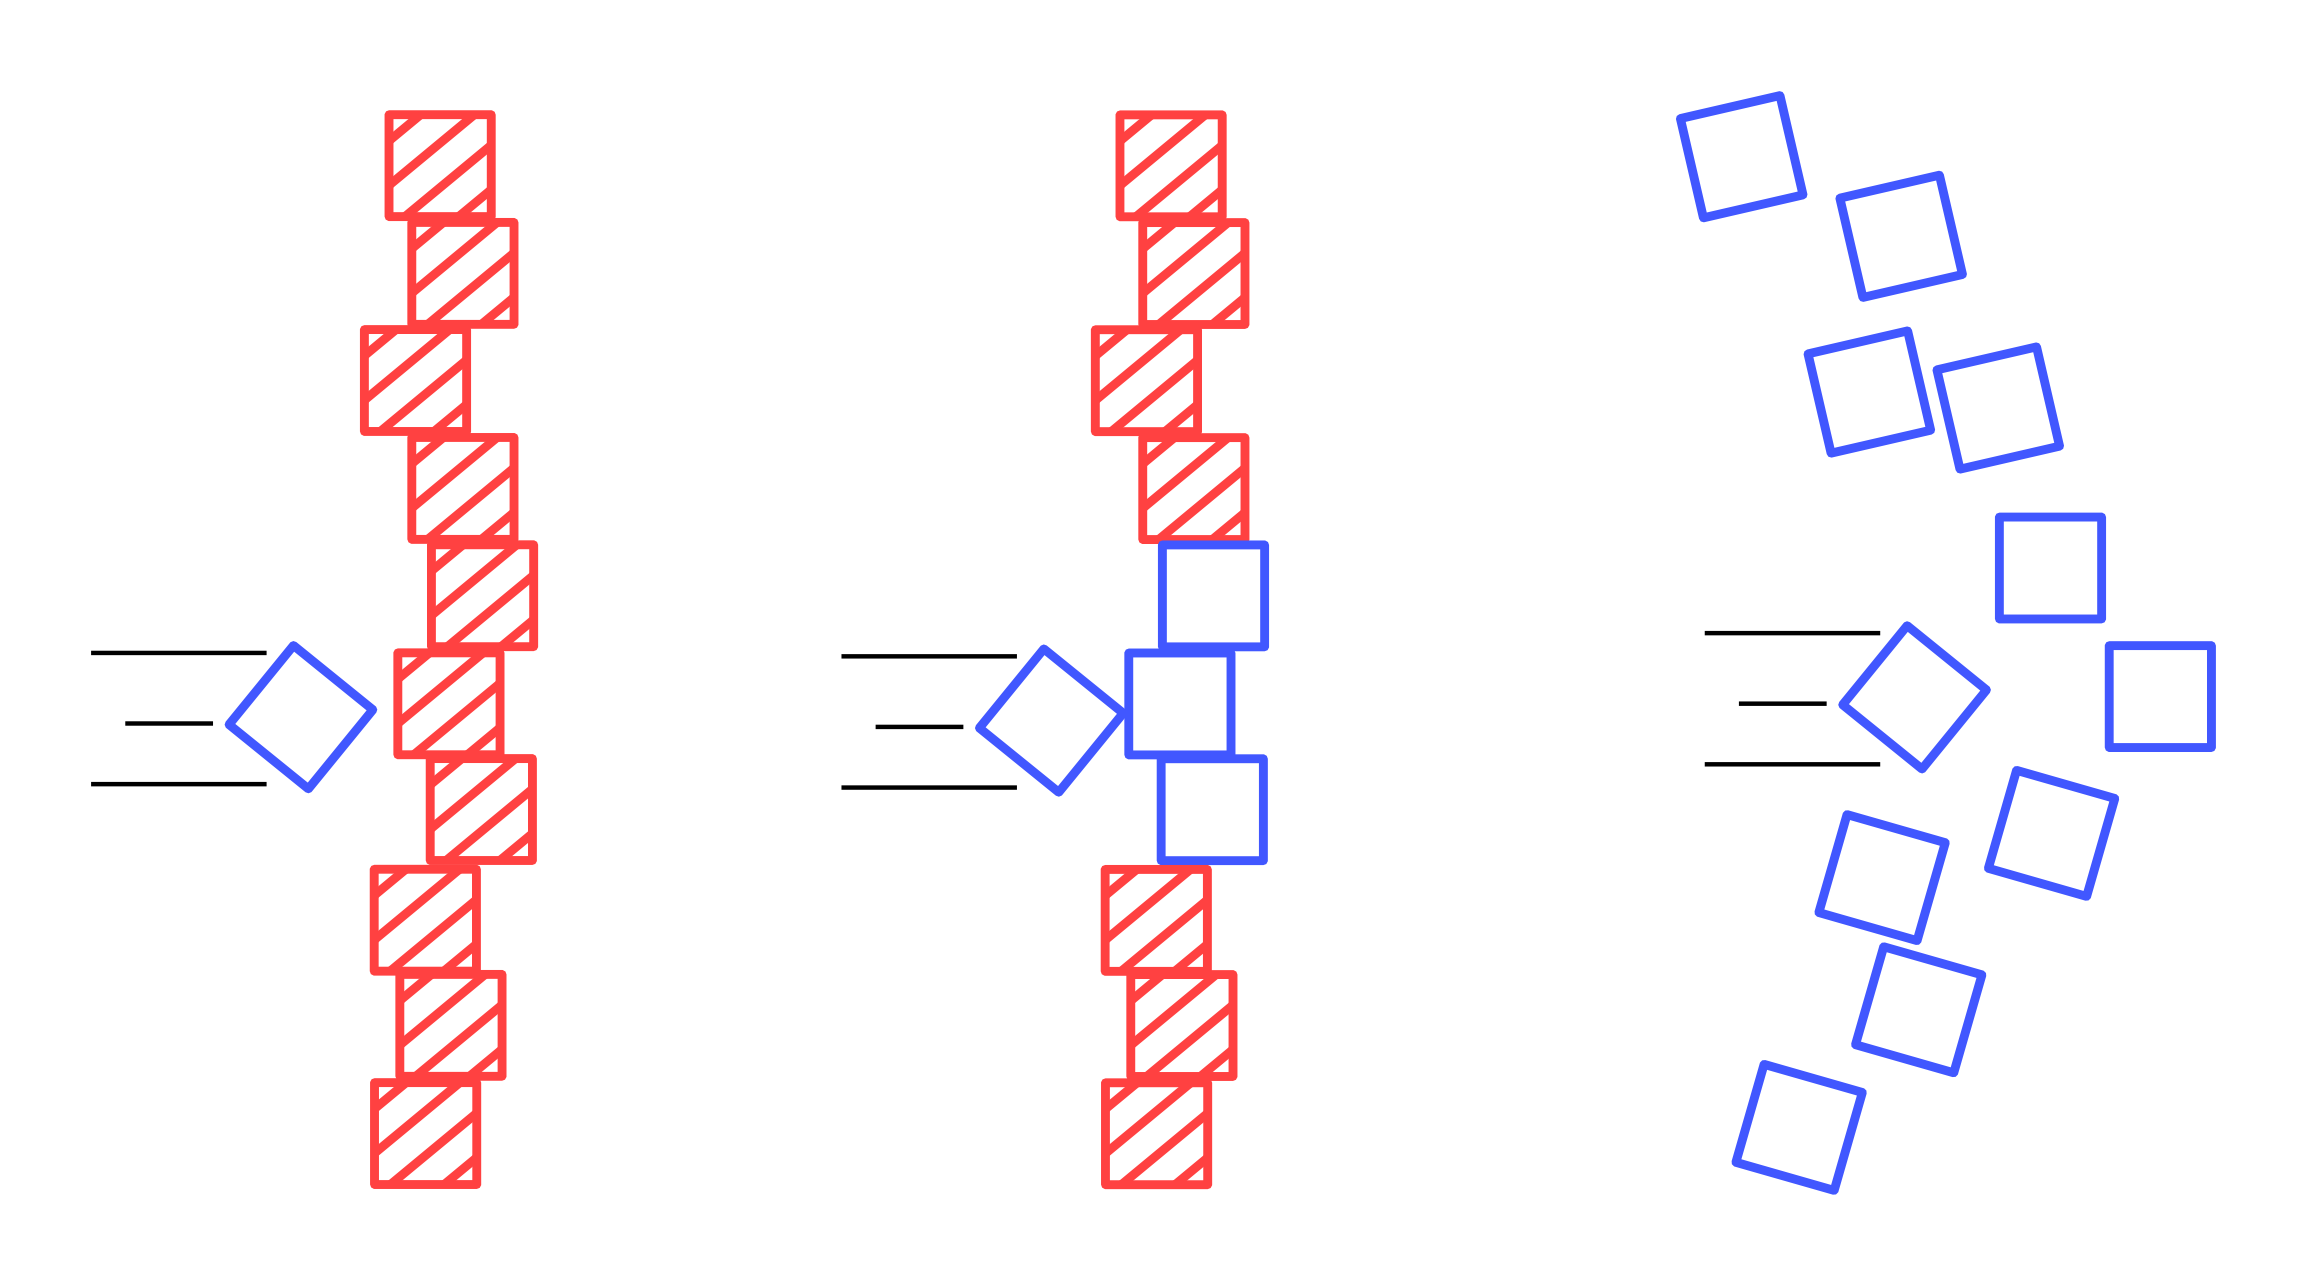
\includegraphics[scale=0.5]{images/starAdaptivity-cgf2016/freezing-rigid.png}
		\caption{\label{fig:stackFreezing}}
	\end{subfigure}
	\hfill
	\begin{subfigure}[b]{0.45\linewidth}
		\centering
		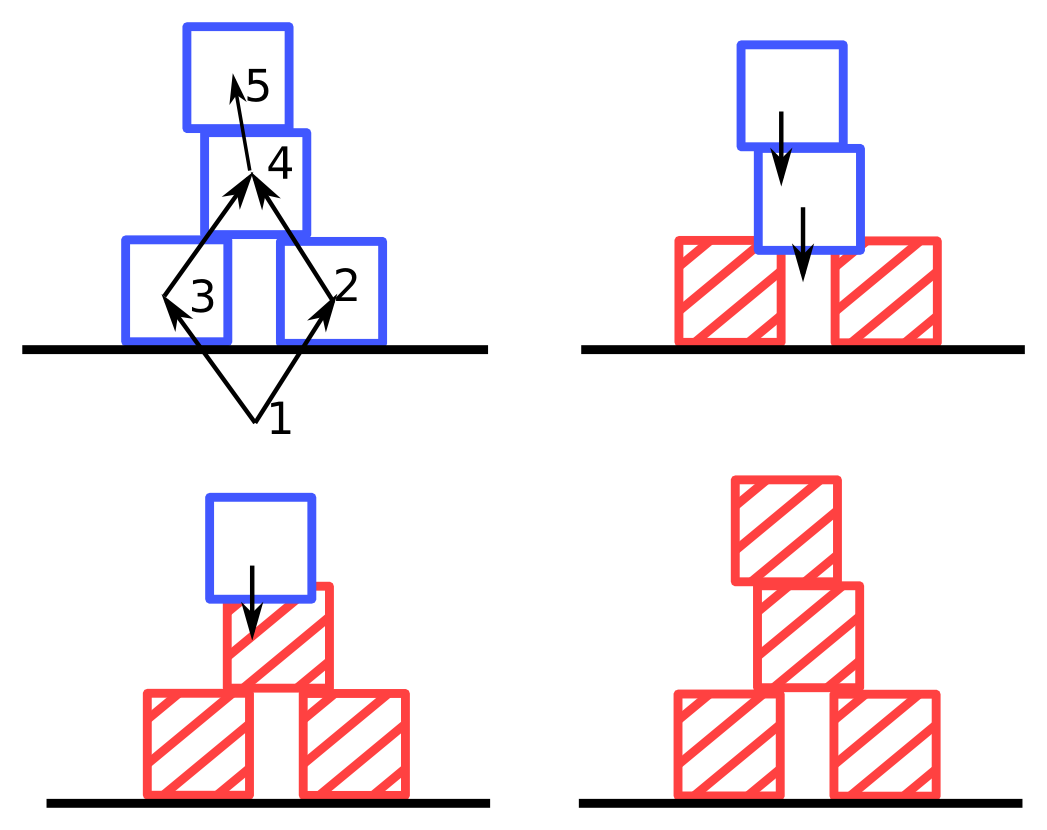
\includegraphics[scale=0.7, angle=0]{images/starAdaptivity-cgf2016/freezing-graph.png}
		\caption{\label{fig:graphFreezing}}
	\end{subfigure}
	\caption[STAR adaptivity: Rigid body freezing]{
		\label{fig:freezingTechniques}
		Freezing techniques applied to rigid bodies stacking. At the stage of contact solving, those methods can save computational time while ensuring a plausible motion.
		In (a), quiescent rigid bodies are frozen (in hatched red) in a stacking configuration. A collision event then awakes one of the rigid bodies, and the active rigid body (in blue) propagates the information to its neighbors.
		In (b), a contact graph stores stack ordering. During shock propagation, a bottom-up traversal is performed and objects at each level are frozen by assigning an infinite mass.
	}
\end{figure}

Freezing techniques have been used as a failsafe procedure for resolving collisions and contact between rigid or deformable bodies.
When many interacting contacts are present, iterative processes for collision response can require an excessively large number of iterations to converge, and early termination leaves the system in an interpenetrating state.
Freezing procedures are attractive in this context as they can guarantee elimination of interpenetrations.
However, they also introduce loss of kinetic energy by treating contacts as fully inelastic, and are therefore only invoked as a last resort after multiple iterations of a physically correct solver have failed to resolve the collisions.
For rigid body contact, Guendelman et al. \cite{Guendelman2003} propose a shock propagation strategy which freezes bodies progressively from the ground up.
They start by building a directed acyclic graph consisting of ``levels'' of objects that are resting on objects of lower levels (cyclic dependencies are grouped into the same level).
A single bottom-up traversal of the graph resolves contacts level by level, assigning infinite mass to lower-level objects for which contact is solved (see Figure \ref{fig:graphFreezing}).
Rigid impact zones, described by Provot \cite{Provot1997} and Bridson et al. \cite{Bridson2002}, are extensively used to resolve collisions in cloth.
Nodes involved in multiple interfering collisions are collected into disjoint sets called ``impact zones'', constructed by merging zones if their nodes are involved in the same node-face or edge-edge collision.
Each impact zone is made rigid by replacing the motion of its nodes with a rigid body motion while preserving the total linear and angular momentum.
This process eliminates collisions within the zone, but may introduce new collisions with nearby elements outside the zone.
Therefore, one must perform collision detection again and grow the impact zones if new collisions are detected, iterating this process until no new collisions occur.
\paragraph*{}
Freezing techniques were also used for articulated rigid bodies, both for dynamics~\cite{Redon2005} and quasi-statics~\cite{Redon2006}: joints are activated or deactivated based on user-defined error metrics, leading to a simplification of the whole model and a sub-linear computational complexity.

Denoting by $\mathbf{\ddot{q}}^C=(\mathbf{\ddot{q}}_1,\ldots,\mathbf{\ddot{q}}_{N_C})^T$
the composite acceleration of an articulated body $C$, where $N_C$ is the number of joints in $C$, the \emph{acceleration
metric value} of $C$ is defined as
\[\mathcal{A}(C)=\sum_{i\in C}\mathbf{\ddot{q}}_i^T\mathbf{A}_i\mathbf{\ddot{q}}_i,\] where $\mathbf{A}_i$, $i\in C$, are symmetric, positive definite $d_{J_i}\times d_{J_i}$ \emph{weight matrices}, and $d_{J_i}$ is
the number of degrees of freedom of joint $i$ in $C$. The weight matrices $\mathbf{A}_i$ are required to depend at most on joint positions, and the simplest choice is the identity
matrix. The key to the sub-linear complexity is the demonstration that the acceleration metric of each sub-articulated body is a quadratic function of the forces applied to its handles (i.e. the free rigid bodies used to assemble sub-articulated bodies in Featherstone's methodology~\cite{Redon2005}). As a result, the acceleration metric may be computed \emph{before computing the joint accelerations themselves}. This is used during the top-down pass of Featherstone's divide-and-conquer algorithm to determine which joint accelerations should be computed because they are sufficiently large~\cite{Redon2005}. For example, if the acceleration metric of the complete articulated body is small, then all joint accelerations are small and joint velocities are constant for the current time step. A similar metric is built for joint velocities to determine which joint positions should remain constant, and thus which inter-body forces and inertial terms should be updated. Once all position-dependent terms are up to date, the motion metrics are available for the next time step, and a new set of active joints can be determined.

It was shown that this approach could also help to speed up continuous collision detection for articulated bodies~\cite{Kim2008Collision} and haptics rendering~\cite{Morin2007}, as well as enable view-dependent articulated-body dynamics by combining motion metrics with visibility estimates~\cite{Kim2008View} (see Figure \ref{fig:ViewDependentArticulatedBodies}).
\begin{figure}[!t]
	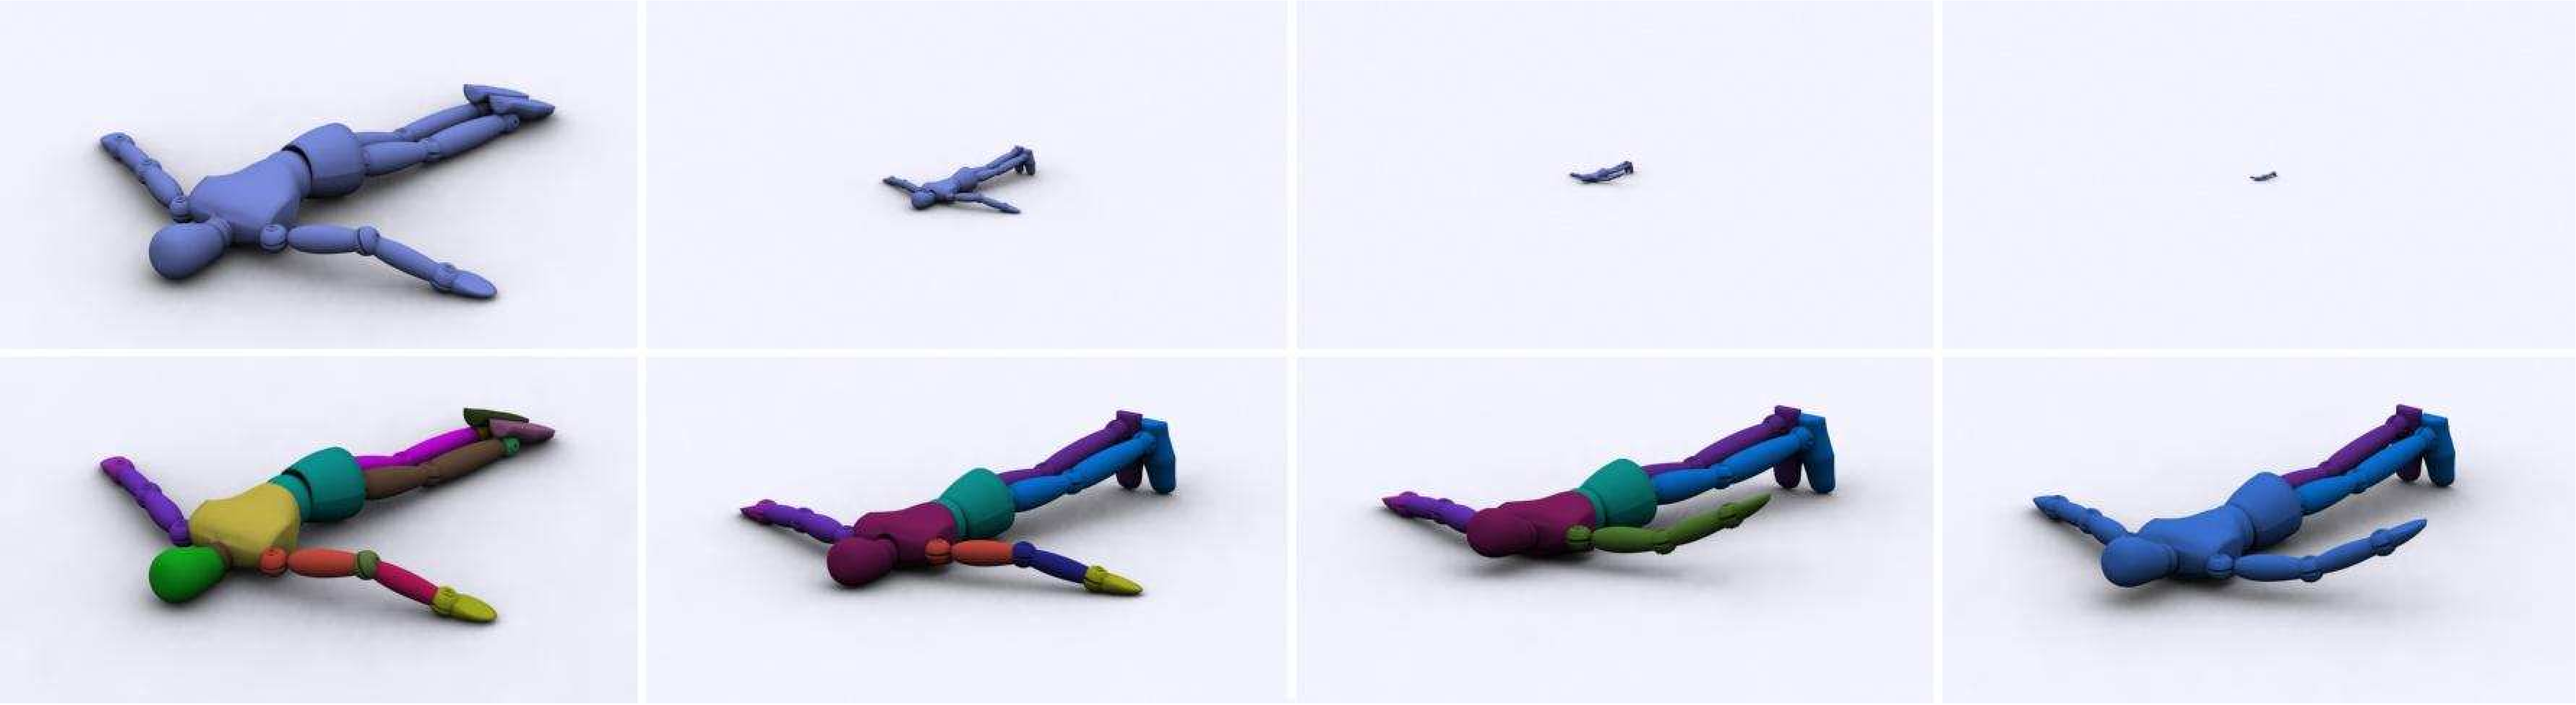
\includegraphics[width=\linewidth]{./images/starAdaptivity-cgf2016/WMComparisonNoLabels.png}
	\caption[STAR adaptivity: Articulated rigid body freezing]{\label{fig:ViewDependentArticulatedBodies}View-dependent dynamics of articulated bodies. Top: the algorithm proposed by Kim et al. \cite{Kim2008Collision} automatically simplifies the dynamics of a falling character as its distance to the viewer increases. Bottom: corresponding rigidification at this time step (one color per rigid group).}
\end{figure}
Gayle et al. \cite{Gayle2006} demonstrate how to perform contact handling with such an adaptive articulated-body method, which is used as the core of a physics-based sampling algorithm for highly articulated chains~\cite{Gayle2007} and cable route planning~\cite{Kabul2007}.
\paragraph*{}
Recent work has sought to apply freezing techniques to accelerate SPH fluid simulation.
In these methods, particles are divided into two sets: a set of \emph{active} particles following a classical simulation step, and a set of \emph{inactive} particles that are skipped in the simulation.
As physical quantities in SPH are interpolated from neighbors, inactive neighbors of active particles also need to be updated to ensure that active particles compute correct physical quantities.
Computation time is saved for inactive particles that only have inactive neighbors.
The main challenge in these methods is the definition of the process to transform a particle from the inactive set to the active one and vice versa.
Indeed, as SPH is sensitive to particle distribution, an inadequate transition of state can directly lead to instabilities.
Additionally, a judicious choice of criterion to decide whether a particle should be active or not is essential.

Goswami and Pajarola \cite{Goswami2011} propose a simple method that evaluates the active status of particles at each time step.
Particles are marked as active if they are close to the boundary or if their velocity exceeds a threshold.
Inactive neighbors of such particles are also added to the active set, and continue with their last active velocity.
All other particles are considered inactive.
Unfortunately, the resulting method does not obey Newton's third law, resulting in some loss of momentum.
In the context of molecular simulation, Artemova and Redon \cite{Artemova2012} propose a fundamentally different approach which ensures momentum conservation. In Chapter~\ref{chap:arps}, we extend their work to computer graphics.

\subsection{Geometric adaptivity} 
\label{sec:spatial_refinement}

Geometric adaptivity describes various techniques that adapt the spatial resolution of a model by refining and coarsening its discretization. These techniques are also referred in the literature as \emph{adaptive spatial refinement}. However, as they include coarsening as well, we adopted a more general term.

Geometric adaptive techniques have two major components: a refinement criterion that determines where higher resolution is needed, and a refinement/coarsening scheme that modifies the discretization to match the desired resolution.
Both physical and visual criteria have been employed in existing work, and we discuss them in more detail below.
The refinement scheme itself essentially depends on the type of spatial discretization.
In the following subsections, we will deal with the three major kinds of discretization separately: structured meshes and grids, unstructured meshes, and meshless models.


\paragraph*{Refinement criteria}
The choice of refinement criteria plays a major role in the quality of the resulting simulation.
Many techniques use simple heuristics such as the distance to boundaries, surface curvature, and the presence of contacts.
However, some authors have shown that employing criteria that are more closely tied to the dynamics of the system can be important in many contexts.

In elastic and plastic solids, the stress and strain in an element characterize the amount of local deformation.
Therefore, the values and gradients of these quantities are often used to control refinement.
Wu et al. \cite{Wu2001} describe several different error estimators of this type and discuss their relative advantages, drawbacks, and performance.
Going beyond estimating a scalar error, Wicke et al. \cite{Wicke2010} define a metric tensor $\mathbf M$ that approximates the spatial variation of strain by comparing deformation gradients of adjacent elements.
The matrix $\mathbf M$ is defined in such a way that it has large eigenvalues in directions in which the deformation changes most rapidly, and can thus be used to control anisotropic refinement (see Figure \ref{fig:Wicke2010}).
\begin{figure}[!t]
  \centering
  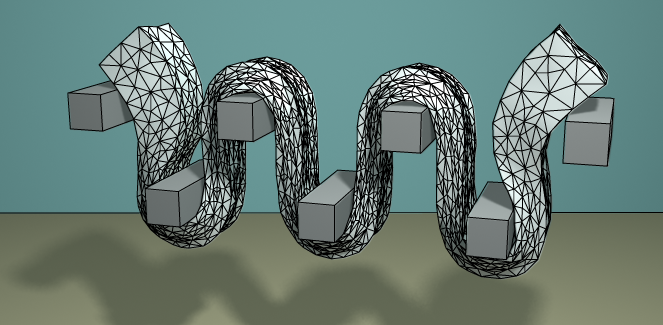
\includegraphics[width=0.8\linewidth]{images/starAdaptivity-cgf2016/mesh-plastic.png}
  \caption[STAR adaptivity: Tetrahedral remeshing]{Elastoplastic simulation with dynamic local remeshing \cite{Wicke2010}. By using the strain gradient as the refinement criterion, regions undergoing severe deformation are refined locally.}
  \label{fig:Wicke2010}
\end{figure}

If a multi-grid algorithm is used, the difference between the solution at the current level, $\mathbf x^j$, and the one prolonged from the next coarser level, $\mathbf P^j\mathbf x^{j+1}$, provides a natural measure of the quality of $\mathbf x^{j+1}$.
Otaduy et al. \cite{Otaduy2007} weigh the error by the local system matrix $\mathbf A$ to reduce possible popping in stiff scenarios, leading to the error metric
\begin{equation}
	e = \|A^j(\mathbf x^j-\mathbf P^j\mathbf x^{j+1})\|,
\end{equation}
and perform refinement if $e$ exceeds a predefined threshold.

Lower-dimensional bodies, like wires, strands, cloth, and thin sheets, undergo not just stretching but also bending (and torsion, in the case of one-dimensional strands).
While the stretching forces within the material are much stiffer than the bending forces, the bending deformation can often be more visually important, and also introduces geometric nonlinearities that must be carefully resolved.
In this context, geometrical curvature and the presence of contacts (which are likely to induce bending) are the most commonly used refinement criteria.
However, the interaction between stretching and bending leads to additional considerations.

First, in the context of cloth simulation, Simnett et al. \cite{Simnett2009} and Narain et al. \cite{Narain2012} point out that elements under compression are likely to buckle and should therefore also be refined, otherwise the wrinkles that would arise in subsequent time steps will fail to be represented on the coarse mesh.
By considering the trade-off between bending and stretching energy, Narain et al. estimate that a sheet under compressive strain $\epsilon$ is likely to form wrinkles of width proportional to $\sqrt{k_b/(k_s\epsilon)}$ where $k_b$ and $k_s$ are the bending and stretching stiffnesses respectively, providing an estimate of the extent of refinement necessary.
In the physics literature, Cerda and Mahadevan \cite{Cerda2003} have provided a detailed semi-analytical analysis of wrinkle geometry that is valid far from the small-deformation limit, and may be useful for future work in graphics.

Second, finer meshes allow higher-frequency modes of transverse oscillation, leading to time step constraints and stability problems that can be fatal for interactive applications.
To ensure stability, Servin et al. \cite{Servin2008} propose a \emph{coarsening} criterion, reducing the resolution of the mesh so that only those oscillations whose frequency is lower than the time stepping rate can be represented.
For simulation of systems with stiff wires, they estimate the maximum frequency of oscillations in a wire discretized with $n$ nodes as
\begin{equation}
	\omega_{\max} \approx 2(n+1)\sqrt{\frac{f}{mL}},
\end{equation}
where $f$ is the tension in the wire and $m$ and $L$ are its mass and length.
Requiring this frequency to be lower than $1/\Delta t$ gives an upper bound on $n$ for each wire.

In fracture simulation, the stress forms a singularity at the crack tip, which must be resolved accurately with a fine resolution mesh for realistic crack paths to be obtained.
If the crack origin is known \textit{a priori}, one can track the crack path as the fracture proceeds and refine the mesh based on the distance from the crack \cite{Busaryev2013}.
However, if fracture is allowed to originate anywhere, it is necessary to refine the mesh wherever stress is sufficiently high, i.e. close to the material's strength $\tau$, because such regions may generate new cracks.
Koschier et al. \cite{Koschier2014} refine elements whose tensile stress $\sigma$ exceeds a specified fraction of $\tau$.
Pfaff et al. \cite{Pfaff2014} choose the desired resolution of the mesh to be proportional to tensile stress by requiring the length of each edge $\mathbf e$ to satisfy
\begin{equation}
	\|\mathbf e\|\le\max\left(\frac{\tau}{2\sigma},1\right)\ell_{\min}
\end{equation}
where $\ell_{\min}$ is a user-specified refinement limit.
This approach allows the mesh to be coarsened again after the crack tip has passed.

It is also possible to perform view-dependent adaptivity by modulating the refinement criteria based on visibility and distance from the camera. Such techniques have been applied to the simulation of wires \cite{Servin2008} and cloth \cite{Koh2014}. New issues arise in such contexts, such as preventing artifacts when coarser regions come into the field of view and must be refined: Koh et al. \cite{Koh2014} achieve this by smoothly increasing the resolution in advance based on the known camera path.

Many adaptive methods for simulation of liquids have relied on the distance to the free surface as the sole refinement criterion.
However, much greater adaptivity is possible by observing that in regions where the surface is flat and does not exhibit detailed motion, it can also be coarsened without significantly affecting the flow.
Adams et al. \cite{Adams2007} propose a purely geometrical criterion based on an ``extended local feature size'' which measures the distance to the surface and to the medial axis of the fluid volume.
This criterion assigns coarse resolution both far from the surface and near thick, flat surfaces.
However, it does not take the motion of the fluid into account.
To detect regions with significant flow detail, Hong et al. \cite{Hong2008FLIP} use a ``deformation factor'' that locally estimates the Reynolds number,
\begin{equation}
  \operatorname{Df} = \frac{(\mathbf u\cdot\nabla)\mathbf u}{\nu\nabla^2\mathbf u},
\end{equation}
where $\mathbf u$ is the fluid's velocity field and $\nu$ is its viscosity.
Ando et al. \cite{Ando2013} use a flexible sizing function that combine multiple criteria to set the desired resolution. Among them the depth of the liquid, the camera viewpoint, the fluid surface curvature and the norm of the strain rate, $e = \|\nabla\mathbf u\|_F$, in order to preserve detailed motions.

\subsubsection{Structured meshes and grids}

\label{sec:structured}
Spatially adaptive simulation techniques can often benefit from symmetry or structure, at the expense of flexibility. Techniques using hexahedral elements or finite differences can use quadtrees or octrees to add spatial adaptivity. Alternatively, techniques that use a volumetric tetrahedral mesh, like some finite element methods or mass-spring systems, can easily take advantage of structured meshes based on lattices. Special techniques can also combine grids with ``tall cells'' or far-field grid structures, as discussed at the end of this section.

The techniques described in this section are useful when one wishes to speed up simulations by using local spatial adaptivity without completely committing to an unstructured mesh technique. Structured meshes often allow more code to be re-used when converting from a regular grid to an adaptive one, and they are often more cache-coherent than fully unstructured meshes. However, structured meshes do not have as much flexibility as unstructured ones.

\paragraph*{Quadtrees and Octrees}
The spatially adaptive schemes of Hutchinson et al. \cite{Hutchinson1996} and Villard and Borouchaki \cite{Villard2005} use quadtrees to directly connect masses and springs, introducing T-junctions in the process. Ganovelli et al. \cite{Ganovelli1999} propose an octree-based multi-resolution method for determining connectivity in a mass-spring system. Debunne et al. \cite{Debunne1999} simulate elastic models using control nodes based on approximate finite differences operators, and they use an octree-based refinement to increase detail based on a Laplacian deformation metric. As discussed in several of the aforementioned works, the main difficulty with using mass-spring models instead of approaches based on continuum mechanics is the notion of {\em convergence}. Convergence is well-studied in the finite element method, and it is trivial to show that increasing spatial resolution will lead to a more accurate solution. Mass-spring models can also converge under refinement if spring stiffness parameters are chosen appropriately, but these stiffness values are not as straightforward to derive compared to the stiffness matrix in a finite element method.

The works of Dick et al. \cite{Dick2011} and Seiler et al. \cite{Seiler2011} use an octree to define a set of hexahedral finite elements in an elasticity simulation, which is specifically used for simulating cuts in a deformable body. Dick et al. also leverage the hierarchy provided by the octree in a geometric multi-grid method for solving the elastodynamics.
The work was subsequently extended to interactively animate high resolution boundary surfaces~\cite{Wu2011}, to improve collision handling~\cite{Wu2013}, and to simulate at haptic rates~\cite{Wu2014}. For more details on methods for cutting deformable bodies, please see the state of the art report by Wu et al. \cite{Wu2015}.

Researchers have also developed octree-based discretizations of the Navier-Stokes equations, which lead to efficient animations of smoke and liquid~\cite{Shi2004,Losasso2004,Losasso2005}.
These approaches also inspired spatially adaptive works that handle discontinuities across free surfaces~\cite{Hong2005}, resolve extremely thin surfaces in bubbles and foam without losing volume~\cite{Kim2007}, and animate multi-phase fluids using regional level-sets~\cite{Kim2010MultiPhase}. More recent work~\cite{Ferstl2014} combines an adaptive hexahedral finite element method based on octrees with a multi-grid Poisson solver to animate highly detailed liquids. Bargteil et al. \cite{Bargteil2006} use octree-based spatial adaptivity to track detailed deforming liquid surfaces using semi-Lagrangian contouring.

It is worth noting that quadtree and octree grid refinement can have subtle side-effects when discretizing partial differential equations. In particular, the regular staggered-grid discretization of the Poisson equation (which is used for enforcing incompressibility in fluid flows~\cite{Bridson2008}) happens to satisfy Stokes' theorem and exactly integrates fluid fluxes --- it doubles as a ``finite volume method'' and can be alternatively derived using discrete exterior calculus \cite{Crane:2013:DGP}. When one replaces the regular grid with an octree, however, it is unsafe to assume that such useful properties will still hold in the presence of T-junctions. The previously-mentioned octree-based fluid simulation methods counteracted this particular problem by carefully designing a new divergence operator, and some researchers observed the emergence of spurious rotational flows when refining an octree near liquid surfaces. 

These subtle problems help explain the large number of adaptive BCC-mesh-based liquid solvers discussed below, which do not exhibit T-junctions.

\paragraph*{Adaptive BCC lattices} A standard way to efficiently generate a tetrahedral mesh with spatial adaptivity is to combine a spatial hierarchy with predefined lattice-based stencils. One particularly popular strategy combines an octree with the body-centered cubic (BCC) lattice tetrahedralization. To give some context, a {\em regular} BCC lattice is defined by first inserting vertices at the corner of a regular cubic grid, inserting additional vertices at the center of every grid cell, and then creating a Delaunay tetrahedralization of these vertices. A {\em spatially adaptive} tetrahedral mesh is created similarly by first creating a weakly-balanced octree (instead of a regular grid), inserting vertices at the corners and centers of the octree cells, and then tetrahedralizing the set of vertices. Please see the work of Molino et al. \cite{Molino2003} and Labelle and Shewchuk \cite{Labelle2007} for some examples of how to create such an octree-based adaptive BCC mesh. This particular meshing strategy has several benefits: the average tetrahedral element has a nearly optimal shape, the quality of the worst element is bounded and completely acceptable in practice, and the computation time required to build the mesh is orders of magnitude faster than unstructured meshes, because it makes use of trees and precomputed stencils.

Employing these ideas, Wojtan and Turk \cite{Wojtan2008} use an adaptive non-conforming BCC tetrahedralization to simulate highly plastic materials while efficiently remeshing whenever element quality degrades (See Figure \ref{fig:WT_BCC}). 
\begin{figure}[!t]
	\centering
	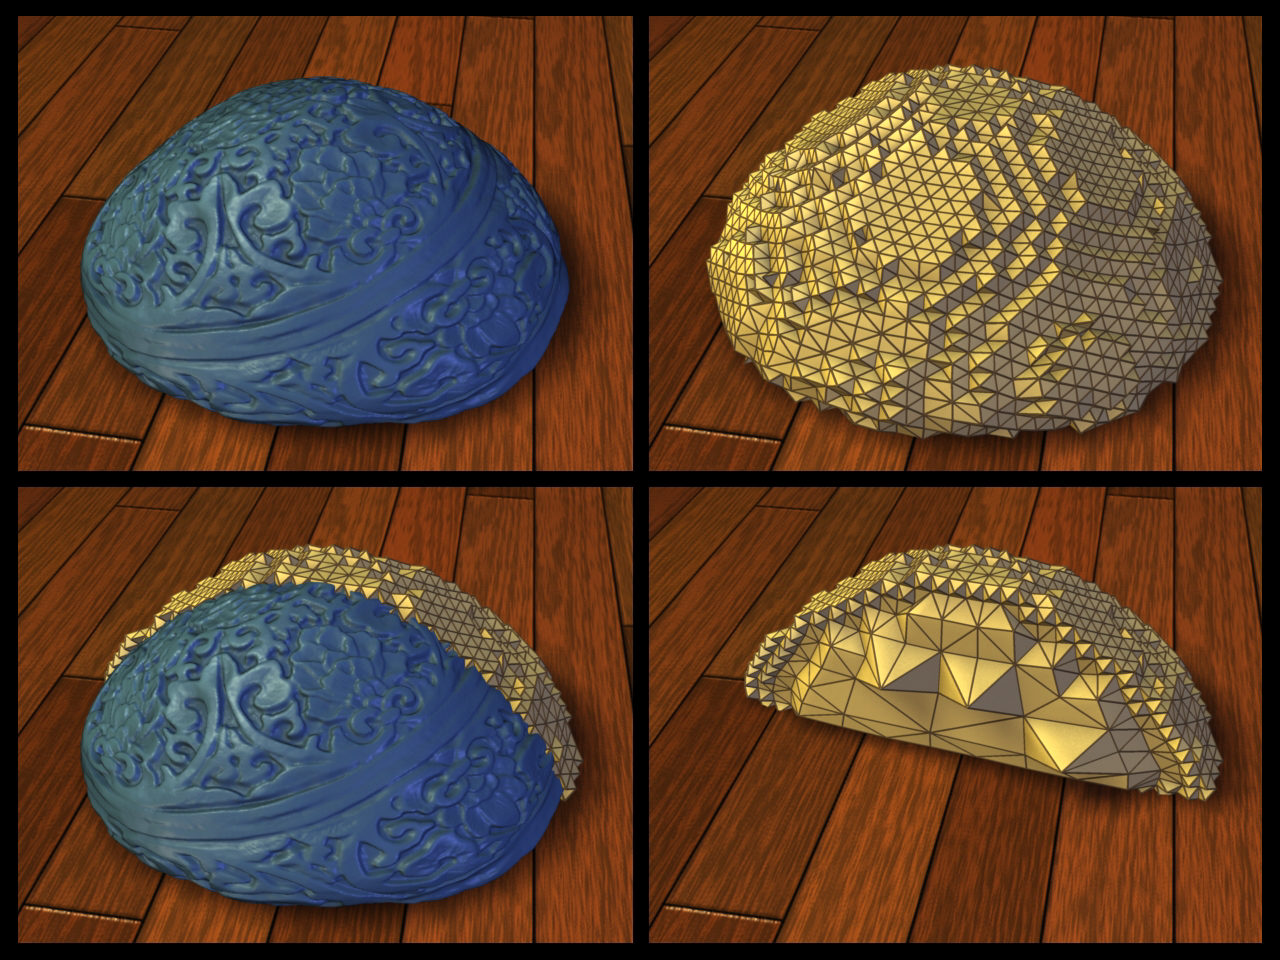
\includegraphics[width=0.8\linewidth]{images/starAdaptivity-cgf2016/WT2008_BCC.png}
	\caption[STAR adaptivity: Body-centered cubic mesh]{A high resolution surface mesh (blue) embedded into a deforming low resolution spatially-adaptive tetrahedral mesh based on a BCC lattice (gold). The bottom row shows the cross section of the tetrahedral mesh, illustrating the BCC structure. Image from Wojtan and Turk \cite{Wojtan2008}.}
	\label{fig:WT_BCC}
\end{figure}
Batty et al. \cite{Batty2010} use a similar meshing strategy to simulate inviscid fluids using a finite-volume discretization. The method also handles embedded solid and free-surface boundary conditions, even though the tetrahedral mesh does not conform to the domain boundaries. Batty and Houston \cite{Batty2011} extend this work by adding an implicit viscosity model. As explained later in the Section \ref{sec:meshless}, Ando et al. \cite{Ando2013} also use an adaptive BCC mesh for simulating liquids. Sifakis et al. \cite{Sifakis2007:Hybrid} introduce the concept of ``hard bindings'' to create an adaptive BCC lattice with T-junctions for the purposes of elastic solid simulation.

Adaptively-refined BCC lattice is exceptionally useful in simulations requiring tetrahedral meshes, because the structured lattice makes the typically expensive operations of remeshing and re-sampling simulation data relatively insignificant. Although the structure of the mesh removes some control over the shapes and nature of the spatial adaptivity, the structure also eliminates typical issues, such as degenerate tetrahedra.

\paragraph*{Tall cell grids} Simulations of deep water also benefit from adaptive ``tall cell'' techniques~\cite{Irving2006,Chentanez2011}, which use regular grid cells near the water surface (where detail and accuracy is important), and tall rectangular fluid cells farther below the surface. This strategy effectively assumes that the behavior in regions located deep underwater is simpler, in that the simulation variables cannot change arbitrarily with depth. While we specifically discuss tall cell grids here because of their use of geometric adaptivity, we will also address some related height-field methods in Section \ref{sec:mixed-models}. These methods seem to work very well when the assumptions of the methods hold. However, there is reason to believe that artifacts (like spurious reflecting waves or dissipating vortices) can occur when the tall cells fail to properly resolve important dynamics.

\paragraph*{Far-field grid structures} Zhu et al. \cite{Zhu2013} propose a method for fluid simulation that maintains an efficient Cartesian grid structure but allows non-uniform spacing between the nodes.
This approach makes it easy to concentrate smaller cells where the domain is more interesting and retain larger cells farther away from areas of interest.
In addition to concentrating detail in important regions, this method also approximates non-reflecting boundary conditions by greatly extending the boundaries of the simulation domain.

\subsubsection{Unstructured meshes}
\label{sec:meshes}
Adaptivity on unstructured meshes is closely related to the problem of remeshing.
Considered purely as a geometrical problem, remeshing has been studied extensively in computational geometry \cite{Cheng2012} and in a modeling context in computer graphics \cite{Alliez2008}.
Indeed, the techniques adopted for adaptive simulation often build on the framework of geometrical remeshing methods, and extend them to a simulation context.
A number of challenges arise when performing remeshing during simulation, though.
First, the mesh elements must remain well-conditioned to avoid degrading the stability of the simulation.
Second, modifying the discretization on the fly risks introducing errors in transferring energy and momentum to the new mesh, such as numerical diffusion due to re-sampling, and discontinuous ``popping'' artifacts in thin strands or sheets.
Third, removing degrees of freedom must be done with care, as a mesh with fewer DOFs cannot represent the previous system state exactly.
Depending on the characteristics of the simulated material---whether it is elastic, plastic, or fluid; whether volumetric or lower-dimensional---different remeshing methods are found to be appropriate.
\begin{figure}[!ht]
	\centering
	\begin{subfigure}[b]{0.2\linewidth}
		\centering
		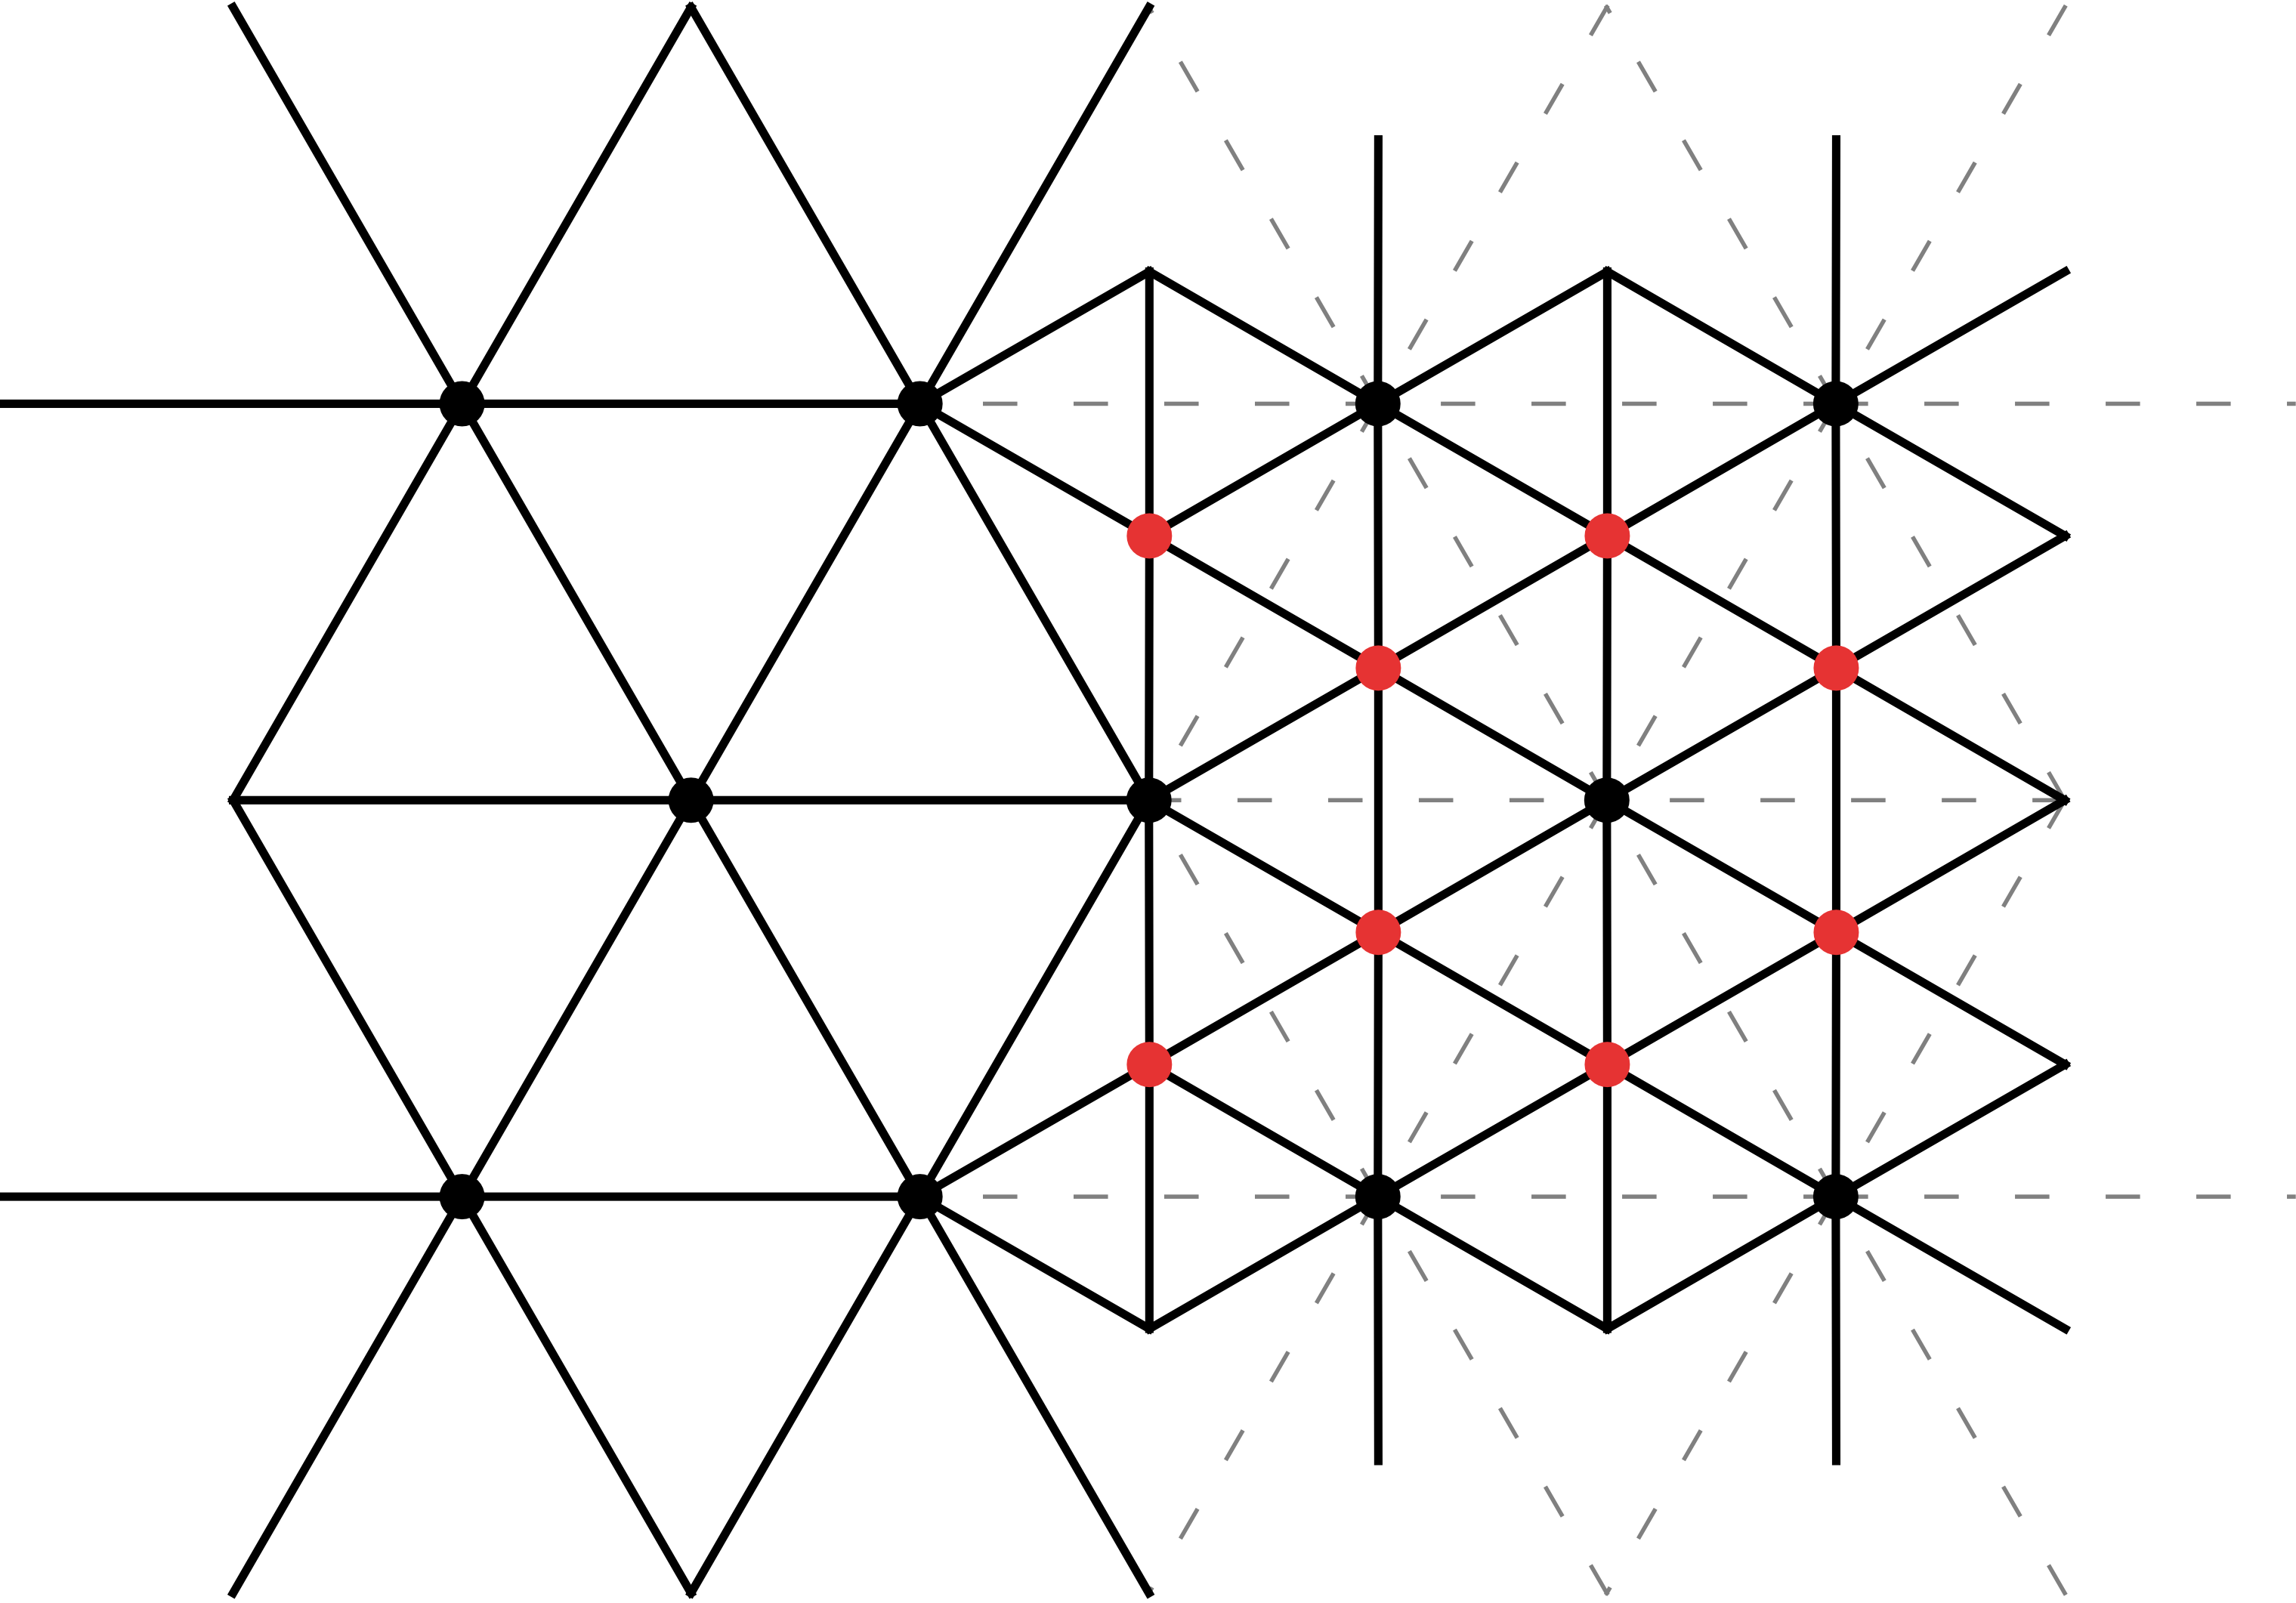
\includegraphics[width=\linewidth,valign=m]{images/starAdaptivity-cgf2016/remeshing-sqrt3.png}
		\caption{\label{fig:remeshing-sqrt3}}
	\end{subfigure}
	\hfill
	\begin{subfigure}[b]{0.2\linewidth}
		\centering
		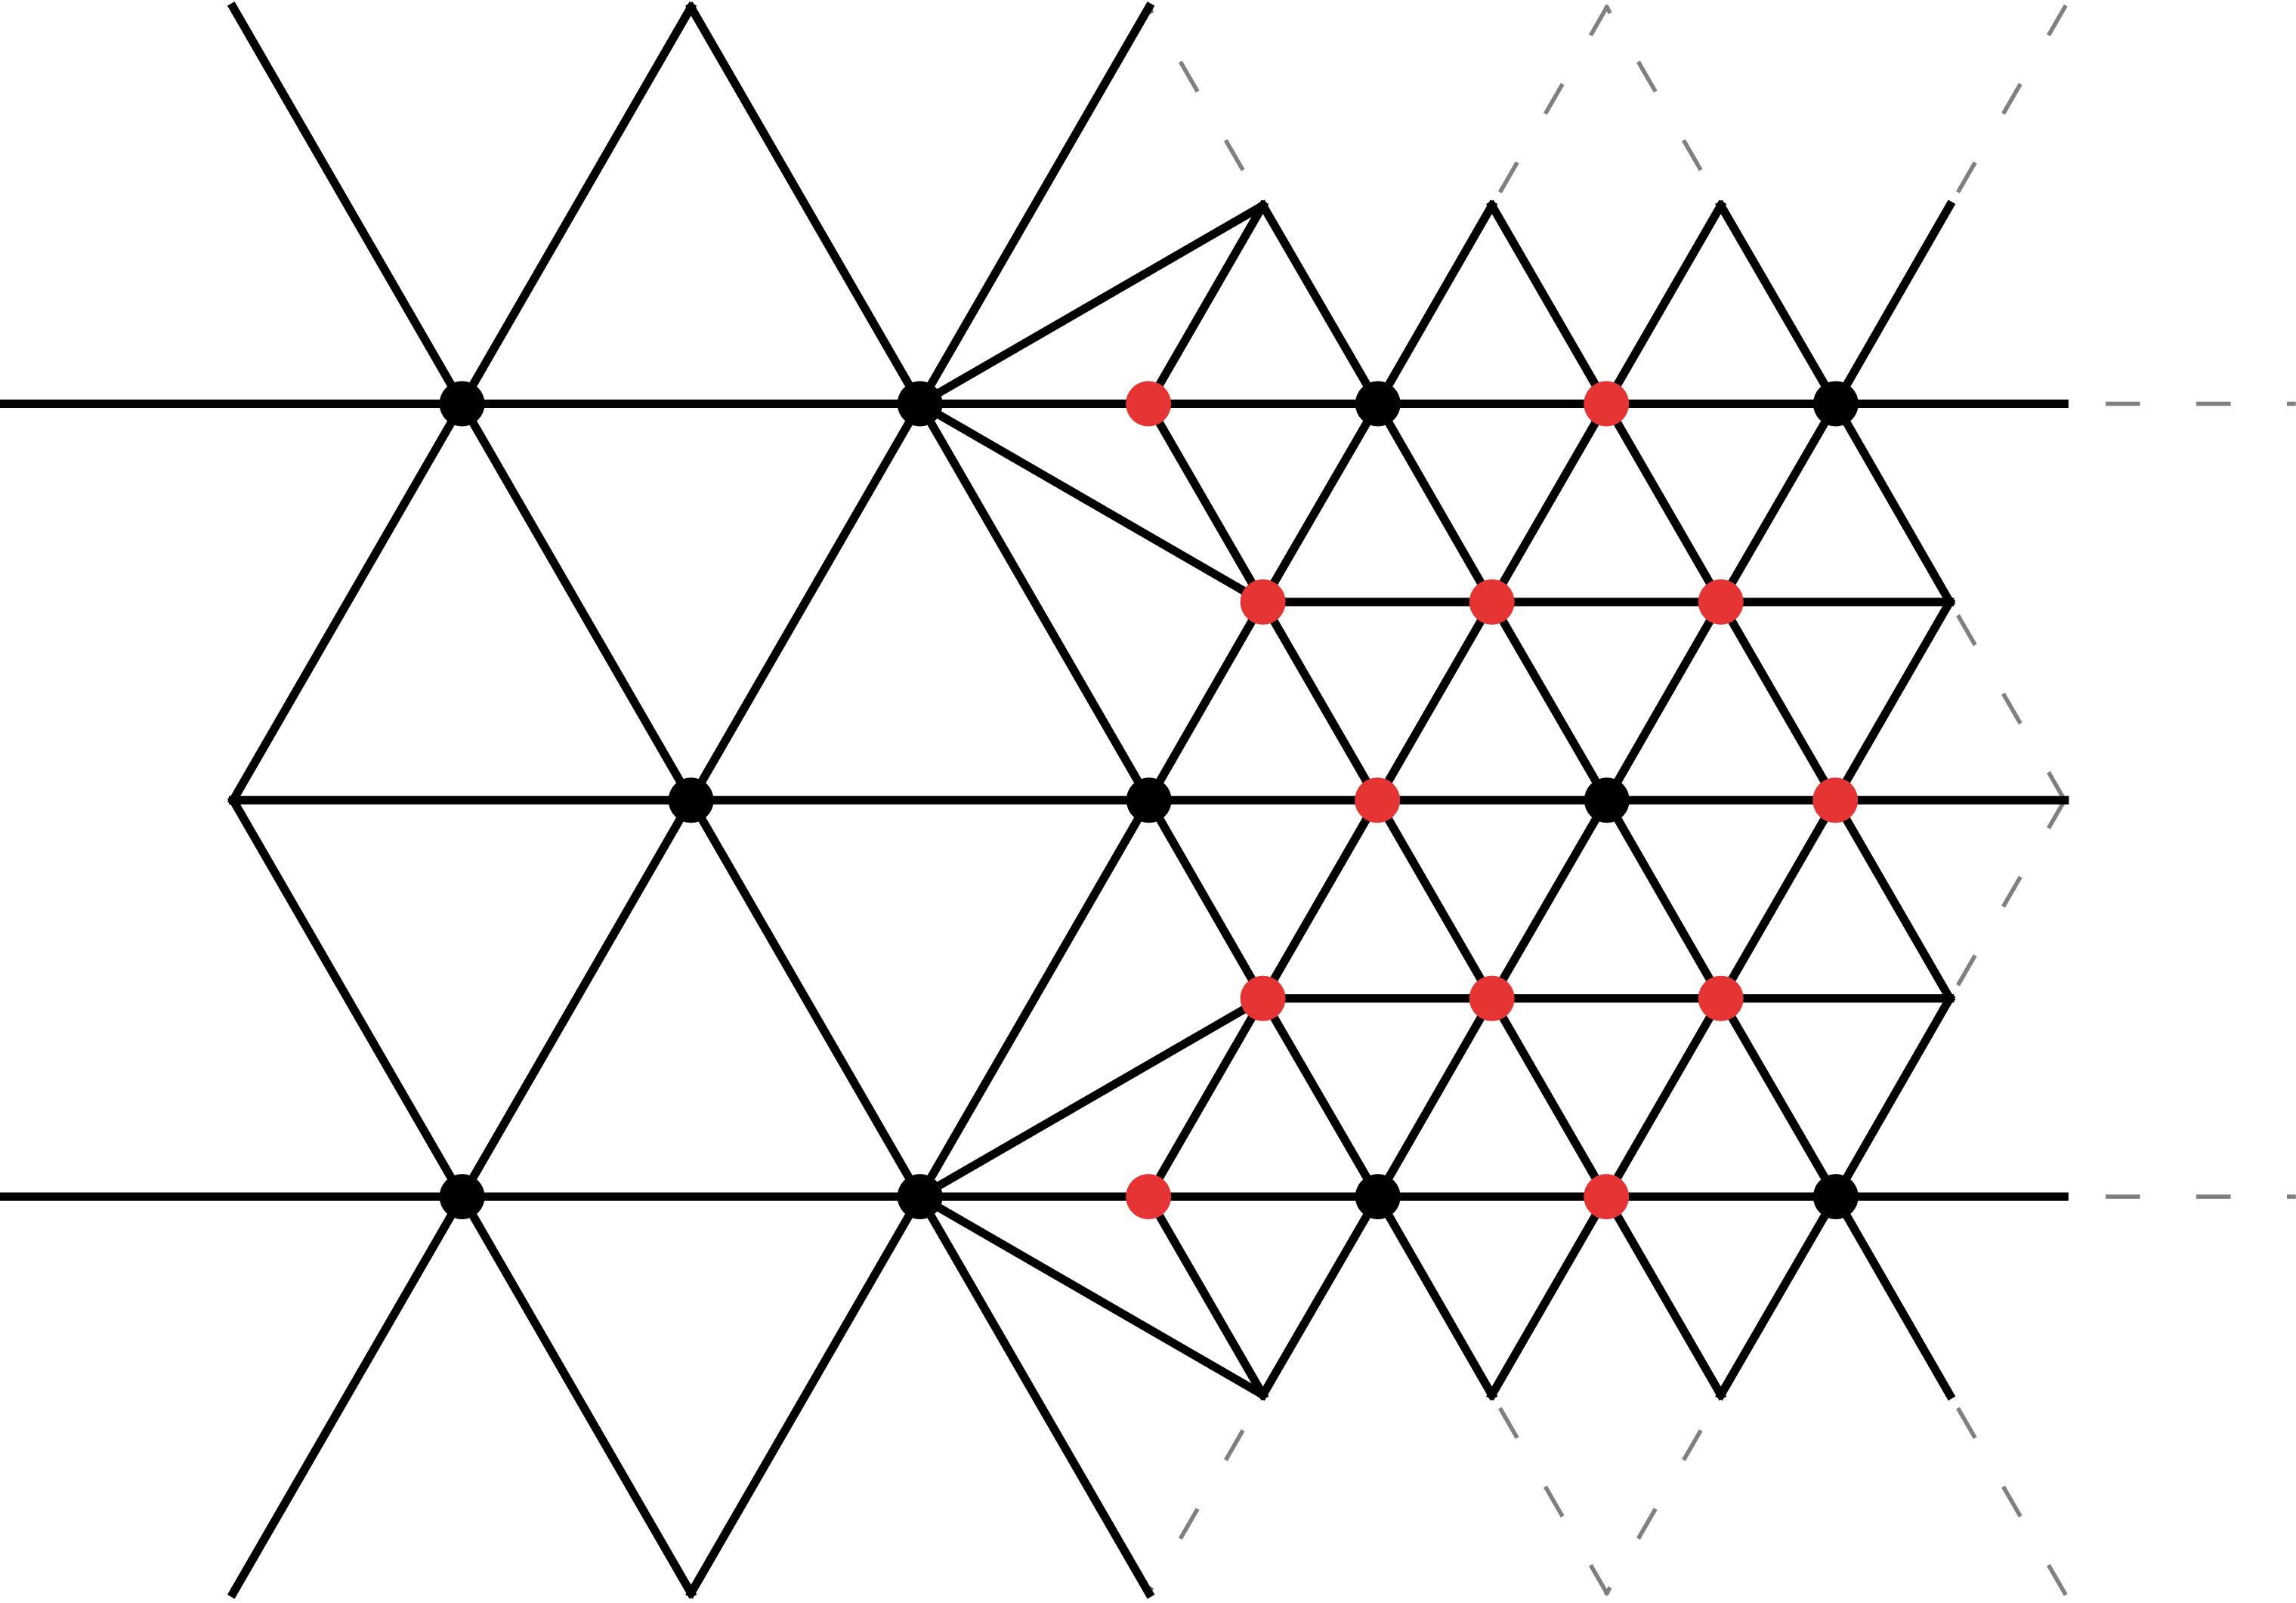
\includegraphics[width=\linewidth,valign=m]{images/starAdaptivity-cgf2016/remeshing-bisect.png}
		\caption{\label{fig:remeshing-bisect}}
	\end{subfigure}
	\hfill
	\begin{subfigure}[b]{0.2\linewidth}
		\centering
		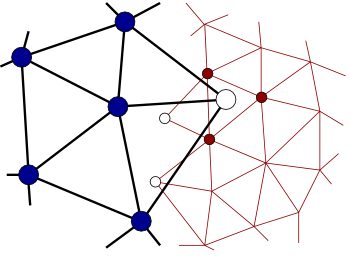
\includegraphics[width=\linewidth,valign=m]{images/starAdaptivity-cgf2016/remeshing-nonnested.png}
		\caption{\label{fig:remeshing-nonnested}}
	\end{subfigure}
	\hfill
	\begin{subfigure}[b]{0.3\linewidth}
		\centering
		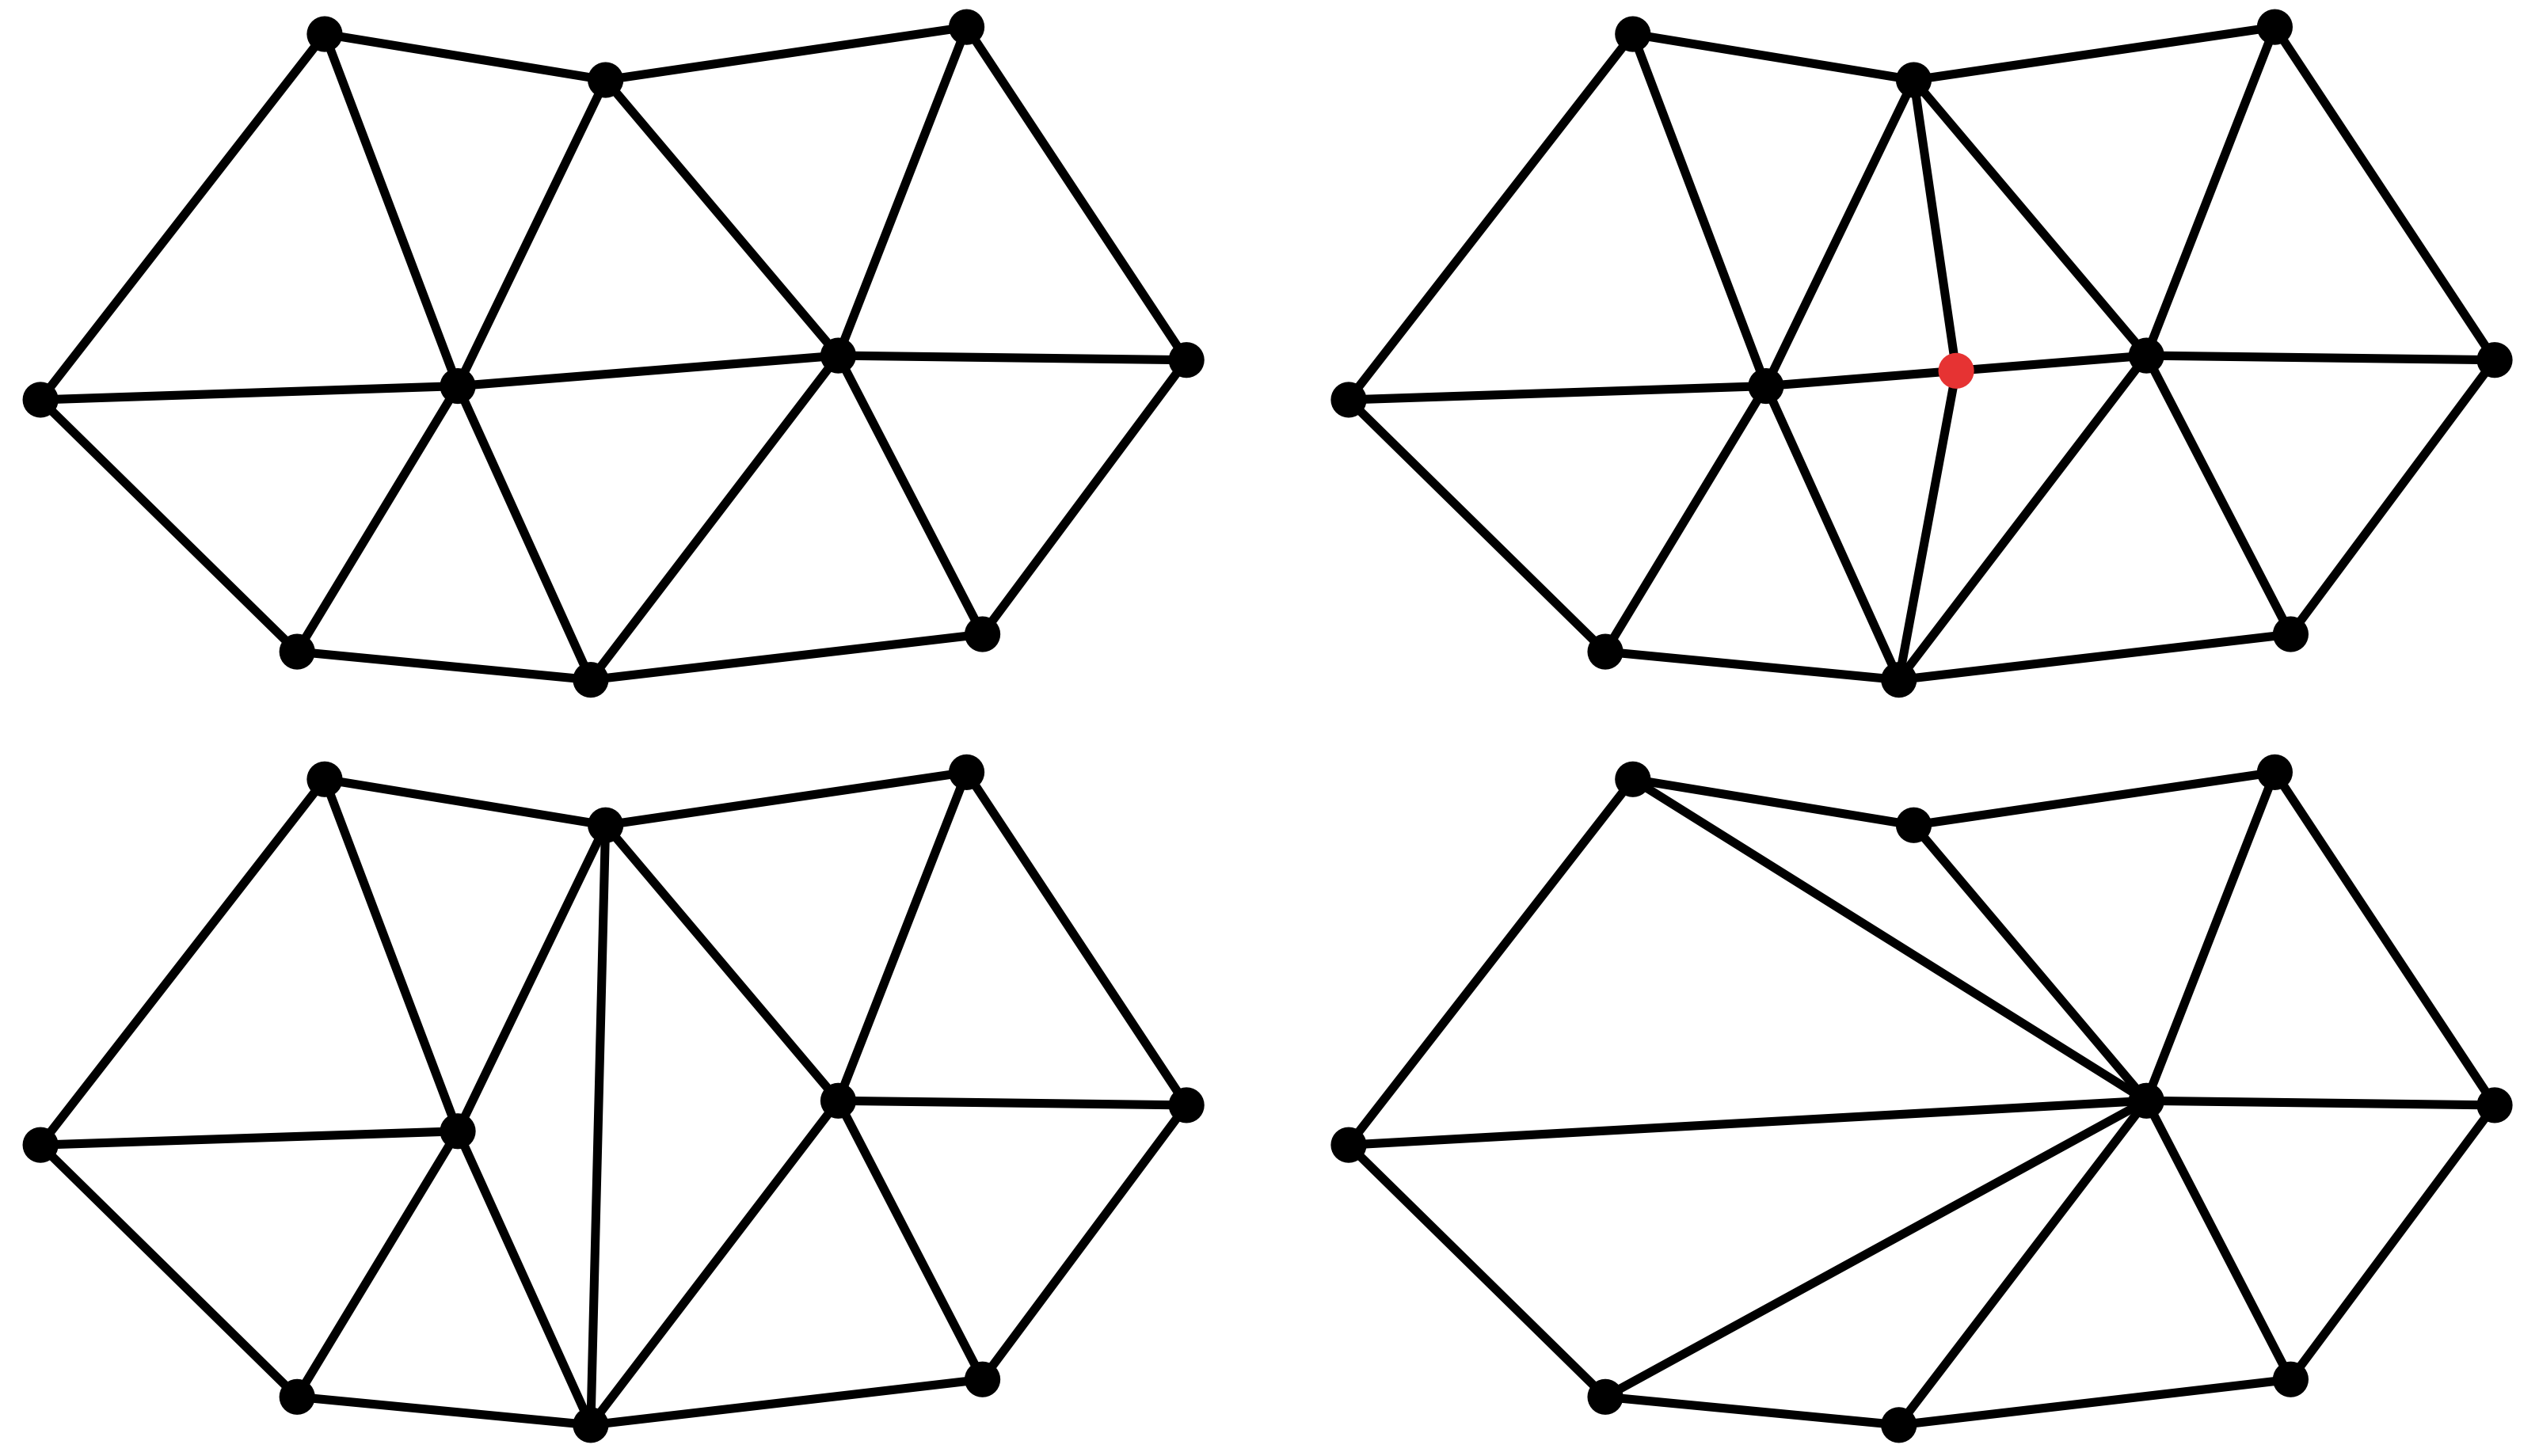
\includegraphics[width=\linewidth]{images/starAdaptivity-cgf2016/remeshing-local.png}
		\caption{\label{fig:remeshing-local}}
	\end{subfigure}
	\caption[STAR adaptivity: Refinement schemes for unstructured meshes]{   \label{fig:remeshing-schemes}
		Overview of refinement schemes for unstructured meshes. In (a) and (b), the right half of a mesh is refined using (a) $\sqrt3$ refinement and (b) hierarchical edge bisection, with inserted nodes highlighted in red. In (c), we illustrate two levels of non-nested meshes. In (d), the three primitive operations of local remeshing are applied to the middle edge: in reading order, we show the original mesh, after an edge split, after an edge flip, and after one of two possible edge collapses.}
\end{figure}
\paragraph*{Hierarchical schemes} The simplest remeshing strategy is to use a fixed hierarchical scheme for refinement, which provides guaranteed bounds on element quality.
Two such schemes are illustrated in Figure \ref{fig:remeshing-sqrt3}, \ref{fig:remeshing-bisect}.
In cloth simulation, triangle subdivision schemes such as 1-to-4 splits, $\sqrt3$ refinement, and edge bisection have been employed \cite{Li2005,Simnett2009,Bender2012:adaptiveFEM}.
A similar scheme for subdivision of tetrahedra was used by Koschier et al. \cite{Koschier2014} for volumetric fracture.
Wu et al. \cite{Wu2001} build on the concept of progressive meshes \cite{Hoppe1996} to precompute FEM parameters, allowing adaptive simulation of deformable bodies at interactive rates.

However, subdivision schemes still degrade element quality by a moderate extent compared to an optimized mesh.
When this is undesirable, an alternative is to use a hierarchy of ``non-nested meshes'' at different resolutions \cite{Debunne2000,Debunne2001}; see Figure \ref{fig:remeshing-nonnested}.
Each level of the hierarchy is a complete mesh that does not necessarily share any nodes with meshes at other levels, and can be independently optimized \textit{a priori}.
At run time, regions at different levels of detail use subsets of different meshes.
Coupling is achieved by allowing the regions to overlap slightly; nodes in the overlap region in each mesh are treated as inactive ``ghost'' nodes that are embedded in the containing element of the other mesh.
The work of Otaduy et al. \cite{Otaduy2007} seamlessly integrates such adaptive non-nested meshes with a multi-grid algorithm and an adaptivity-aware collision detection technique.

Hair simulation can benefit from adaptivity, as the contact interactions between hair strands lead to the formation of emergent clusters.
Bertails et al. \cite{Bertails2003} introduce a hierarchical structure called an adaptive wisp tree (AWT), which represents hair clusters that can progressively split into smaller clusters from the base to the tip.
Refinement is performed by splitting a node if its size and acceleration are large, while coarsening is performed by merging sibling nodes if they have similar positions and velocities.

\paragraph*{Nearly regular meshes}
Some techniques for liquid simulation use a structured mesh in the interior of the volume, but allow irregularities at boundaries to better capture the dynamics of the free surface.
These techniques benefit from many of the advantages of structured meshes discussed in Section \ref{sec:structured}, while still retaining much of the flexibility of unstructured meshes, such as the ability to accurately match boundary conditions.

In such methods, one typically maintains a high-resolution representation of the surface as a triangle mesh that is updated at each time step.
The surface is superimposed on a regular mesh structure such as an octree or a uniform grid, and elements near the surface are modified, or new elements inserted, to better conform to the surface.
In particular, Chentanez et al. \cite{Chentanez2007} use the isosurface stuffing algorithm \cite{Labelle2007} that generates an adaptive BCC lattice whose surface tetrahedra are warped and possibly subdivided to conform to the surface geometry.
Using an octree to construct the lattice allows for coarser resolution away from the free surface.
Brochu et al. \cite{Brochu2010} use a uniform background lattice and introduce additional pressure samples along both sides of the free surface to ensure that all surface features are resolved.
The pressure projection is then performed on a mesh consisting of the Voronoi cells of these sample points.

\paragraph*{Local remeshing}
In some contexts, it is desirable to allow the connectivity structure of the mesh to be modified freely during the course of the simulation.
Such a requirement arises when anisotropic elements are needed to resolve strongly directional features, or when the material exhibits both elastic properties and unbounded deformation, such as in plastic flow.

While it is possible to perform global remeshing---that is, simply creating a new simulation mesh from scratch whenever needed \cite{Klingner2006,Bargteil2007}---this approach can lead to undesirable diffusion of stored physical quantities such as plasticity information.
An increasingly popular alternative is to remesh locally using a set of local operations that refine, coarsen, and reshape existing elements.
In local remeshing techniques, any elements in the mesh that do not satisfy the desired size and shape criteria are improved by careful application of these operations.
This process is repeated until all mesh elements are satisfactory.

When performing remeshing, it is important to ensure that the mesh remains well-conditioned for simulation, through the use of various element quality measures \cite{Shewchuk2002}.
In 2D, the Delaunay triangulation optimizes several important notions of mesh quality, including the minimum angle and the maximum circumradius of any triangle, but the Delaunay tetrahedralization in 3D provides few such guarantees, and more sophisticated mesh improvement strategies may be required \cite{Wicke2010}.
If anisotropic remeshing is desired, the remeshing criterion is often expressed through a spatially varying metric tensor $\mathbf M$, with the goal being that each edge $\mathbf e$ should have $\mathbf e^T\mathbf M\mathbf e\approx1$.
Equivalently, we desire $\|\mathbf M^{1/2}\mathbf e\|\approx1$; that is, we want edges to be of unit length and elements to be equilateral in the transformed space of $\mathbf M^{1/2}$.
This viewpoint allows element quality metrics and Delaunay properties defined for isotropic meshes to be carried over to the anisotropic setting.

For manifold triangle meshes, high-quality remeshing can be accomplished using only the three simple operations of edge split, edge collapse, and edge flip (see Figure \ref{fig:remeshing-local}).
Narain et al. \cite{Narain2012} use these operations in cloth simulation, generating an adaptive anisotropic mesh that resolves detailed wrinkles and folds (see Figure~\ref{fig:Narain2012}).
\begin{figure}[!t]
	\centering
	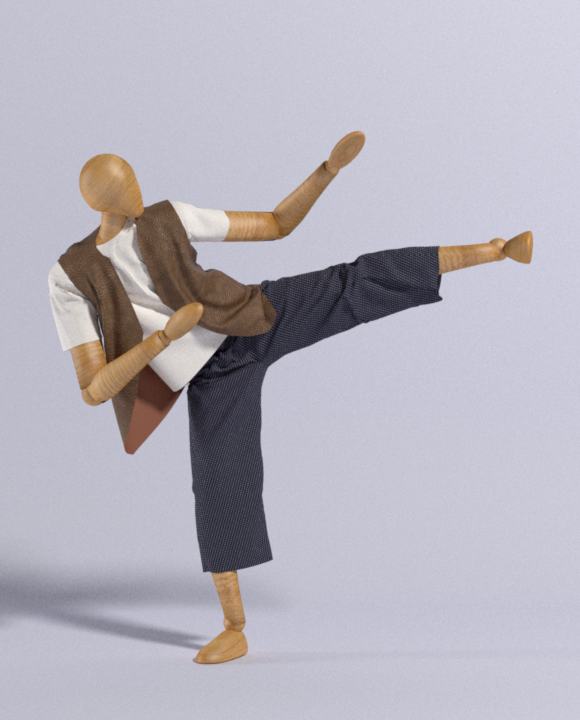
\includegraphics[width=0.35\linewidth]{images/starAdaptivity-cgf2016/cloth-render.png}
	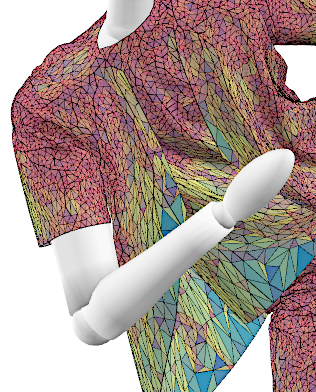
\includegraphics[width=0.35\linewidth]{images/starAdaptivity-cgf2016/cloth-wire-zoom.png}
	\caption[STAR adaptivity: Anisotropic remeshing of triangular meshes]{The anisotropic remeshing algorithm of Narain et al. \cite{Narain2012} allows detailed wrinkles in cloth to be resolved accurately with fine elements (red), while much coarser elements (blue/green) are used in flat regions. Long, narrow folds are best represented using anisotropic elements (yellow) aligned with the curvature direction.}
	\label{fig:Narain2012}
\end{figure}
First, all edges that are unacceptably long according to the refinement criterion are split, then edge collapses are attempted as long as they do not create new unacceptable edges.
During both steps, edge flips are performed to maintain an approximately Delaunay mesh relative to the anisotropic metric.

Local remeshing of tetrahedral meshes is significantly more involved, requiring several different local operations and a complex schedule for the order in which to apply them \cite{Klingner2007}.
This technique was first applied to simulation by Wicke et al. \cite{Wicke2010}, who used it to minimize artificial diffusion in elastoplastic flow.
Subsequent work has applied such remeshing techniques to simulation of incompressible liquids \cite{Misztal2012a,Misztal2012b,Clausen2013}.

Misztal et al. \cite{Misztal2012a,Misztal2012b} build a mesh over the entire simulation domain, with some elements belonging to the fluid and the rest to the exterior, while Clausen et al. \cite{Clausen2013} mesh only the fluid volume.
The former approach allows topological changes like collisions to be handled automatically without special treatment, although at the cost of maintaining a mesh over a potentially much larger domain.
Clausen et al. also describe techniques for guaranteeing incompressibility and momentum conservation that are applicable to both approaches. 
Two key advantages offered by these methods are that (i) the advection step causes no numerical diffusion, because physical quantities move with the mesh nodes, and that (ii) surface tension can be modeled accurately thanks to an explicit surface representation tied directly to the simulation mesh.

Apart from simply adding or removing vertices, surface tracking algorithms in fluid dynamics may also move vertices along the surface in order to optimize mesh shapes.
A process called ``null-space smoothing'', which slides vertices within the tangent space of a meshed surface, is used in several works \cite{Jiao2007,Brochu2009,Brochu2010,Wicke2010,Clausen2013}.
This strategy improves the quality of simulation elements without changing the shape of the tracked surface.

\paragraph*{Additional challenges and techniques}

When refinement is performed, the position of the newly inserted node has to be chosen carefully.
Simply placing it at the midpoint of the original element can cause physical quantities such as bending to change discontinuously, injecting artificial energy into the system and leading to instabilities.
Instead, it is better to adjust the mesh locally to bring it into an energy-minimizing configuration.
Spillmann and Teschner \cite{Spillmann2008} consider the positions of the new node $\mathbf x_i$ and its neighbors as variables and perform an optimization to minimize the total energy,
\begin{equation}
	U(\mathbf x_1,\ldots,\mathbf x_n) - \sum_{j=1}^n\mathbf f_j^T\mathbf x_j,
\end{equation}
where $U$ is the internal energy due to elastic forces, and $\mathbf f_j$ is the external force acting on node $j$.
A similar approach has been used for simulating the behavior of stiff two-dimensional sheets such as paper and metal \cite{Narain2013,Pfaff2014}, but with $\mathbf f_j$ replaced with an acceleration-corrected term $\mathbf f_j - m_j\mathbf a_j$ to preserve the instantaneous acceleration of each node.
\\
Liquids with surface tension may freely transition between volumes, thin films, filaments, and droplets; representing these transitions is a challenge for most mesh-based techniques.
Zhu et al. \cite{Zhu2014} address this problem using non-manifold meshes of mixed dimensionality, composed of tetrahedra, triangles, segments, and points.
Beyond the traditional remeshing operations that work within a single dimensionality, they also provide operations for dimensionality transitions via element collapse (e.g. transforming a thin triangle to a segment) and merging (e.g. generating a tetrahedron to connect two adjacent triangles with small dihedral angle).

Finally, we point out the recent ``power particles'' technique of de Goes et al.~\cite{deGoes2015}, which builds an unstructured mesh at each time step using a Voronoi-style power diagram.
This can be viewed as a global remeshing approach like the ones mentioned above \cite{Klingner2006,Bargteil2007}, but this method stores physical quantities on Lagrangian particles without maintaining an explicit connectivity, and thus avoids numerical diffusion due to re-sampling.
While this work is not specifically an adaptive strategy, it is a form of spatial discretization that makes adaptivity very easy to implement, and could be a fruitful basis for future work in adaptive simulation.

\subsubsection{Meshless models}
\label{sec:meshless}
In the last two decades, numerous meshless models have been extended to perform adaptive physically-based animation. They include Smoothed-Particle Hydrodynamics (SPH) (see the survey of Ihmsen et al. \cite{Ihmsen2014:STAR}), fluid-implicit particle (FLIP) (see the seminal work of Zhu and Bridson \cite{Zhu2005}), moving least squares (MLS) (see Muller et al. \cite{Muller2004:melting}) and frame-based models (see Gilles et al. \cite{Gilles2011}). These models were used to describe a wide range of phenomena, from fluids (SPH, FLIP) to solids (MLS, frame-based).

Due to the absence of fixed connectivity, meshless models are among the most flexible models for spatial adaptivity. This flexibility, combined with the variety of models, leads to an impressive number of re-sampling strategies, developed to resolve details near splashes, large deformations, viscoplastic flows and fractures. We classify these strategies into three categories: (1) dynamic local re-sampling, (2) multi-scale methods, and (3) hierarchical refinement (see Figure \ref{fig:particleOverview}).
\begin{figure}[t]
	\centering
	\begin{subfigure}[b]{0.20\linewidth}
		\centering
		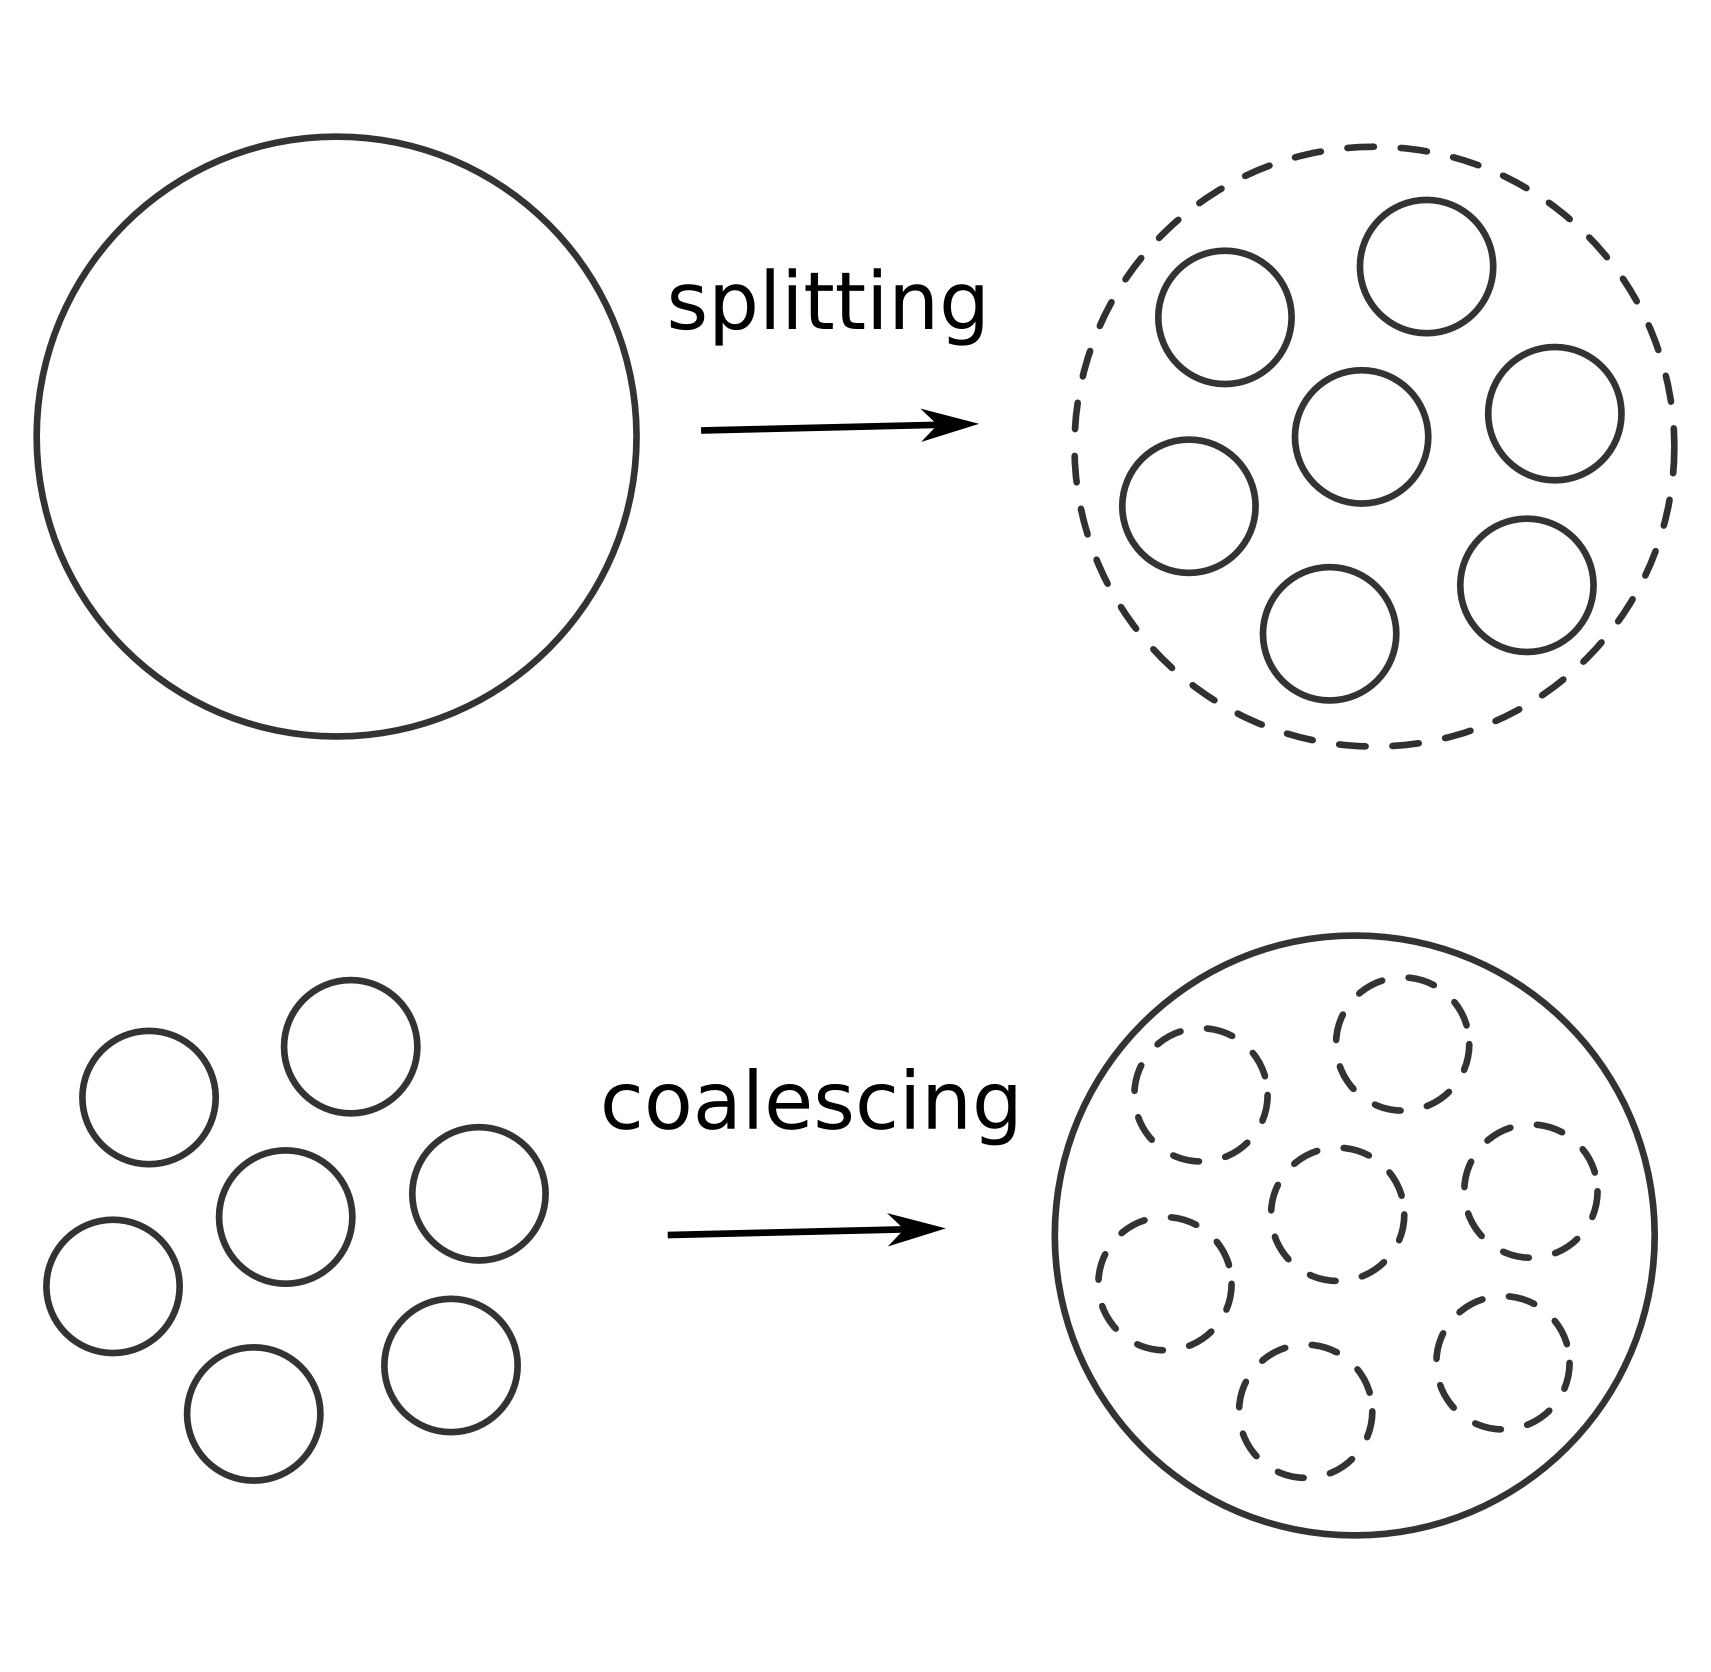
\includegraphics[width=\linewidth]{images/starAdaptivity-cgf2016/particles-operators.png}
		\caption{\label{fig:meshless-operators}}
	\end{subfigure}
	\hfill
	\begin{subfigure}[b]{0.45\linewidth}
		\centering
		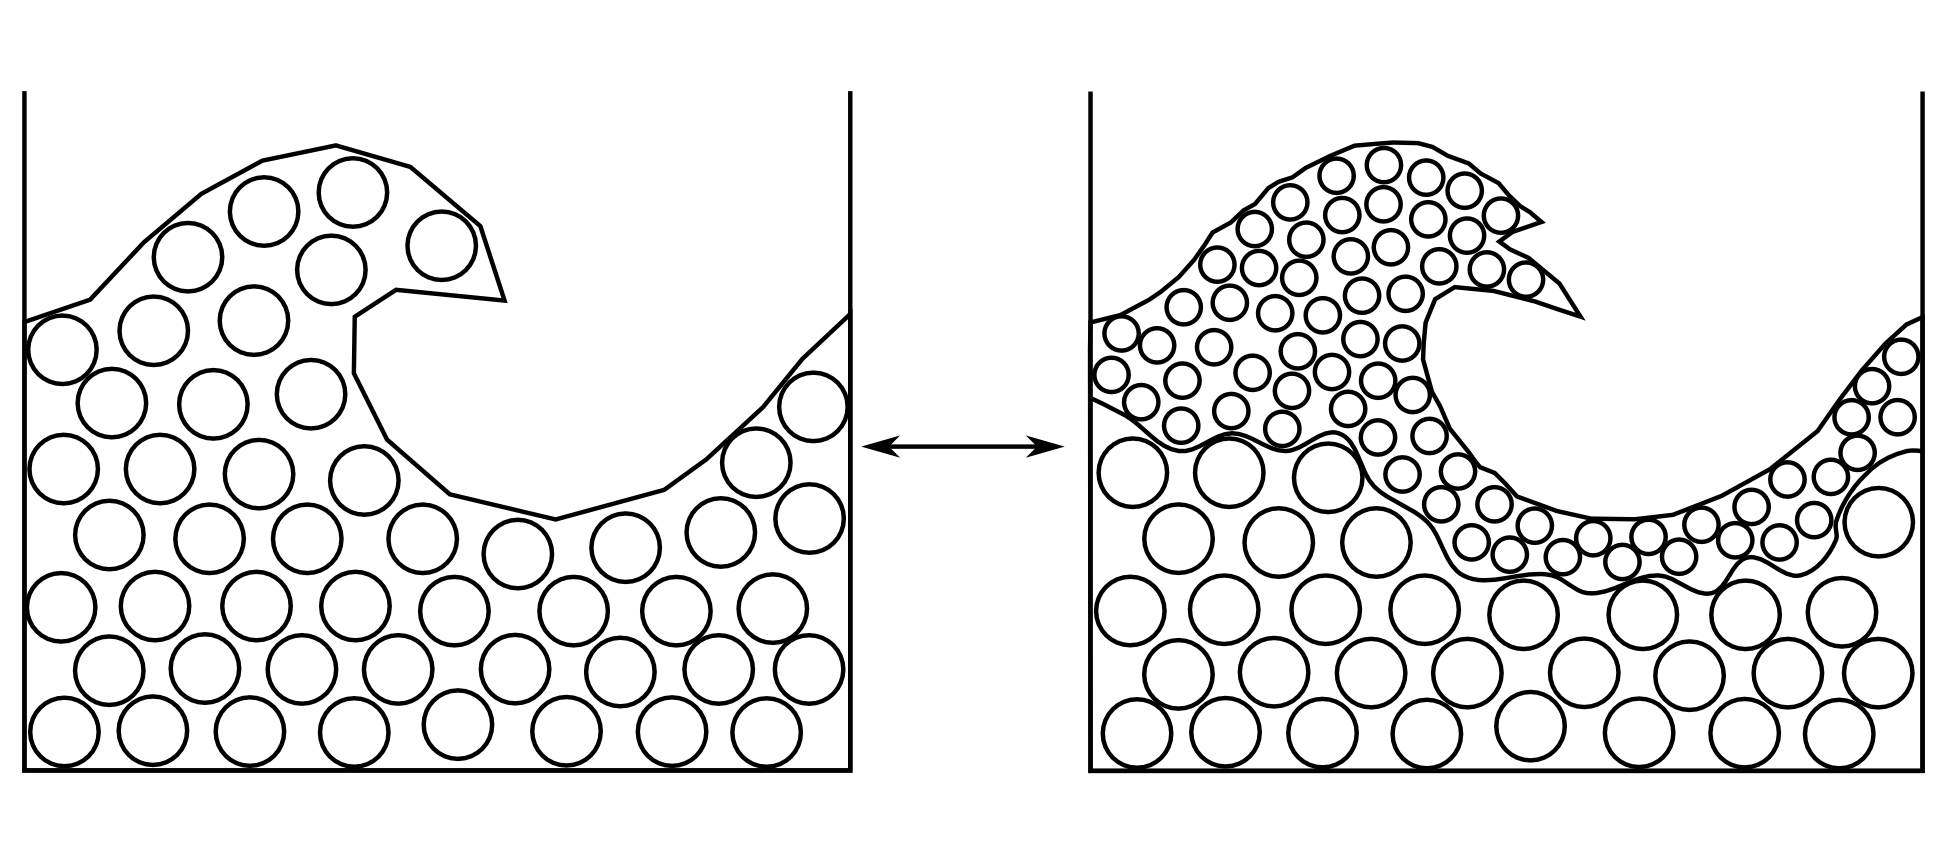
\includegraphics[width=\linewidth]{images/starAdaptivity-cgf2016/particles-multiscale.png}
		\caption{\label{fig:meshless-multi-scale}}
	\end{subfigure}
	\hfill
	\begin{subfigure}[b]{0.3\linewidth}
		\centering
		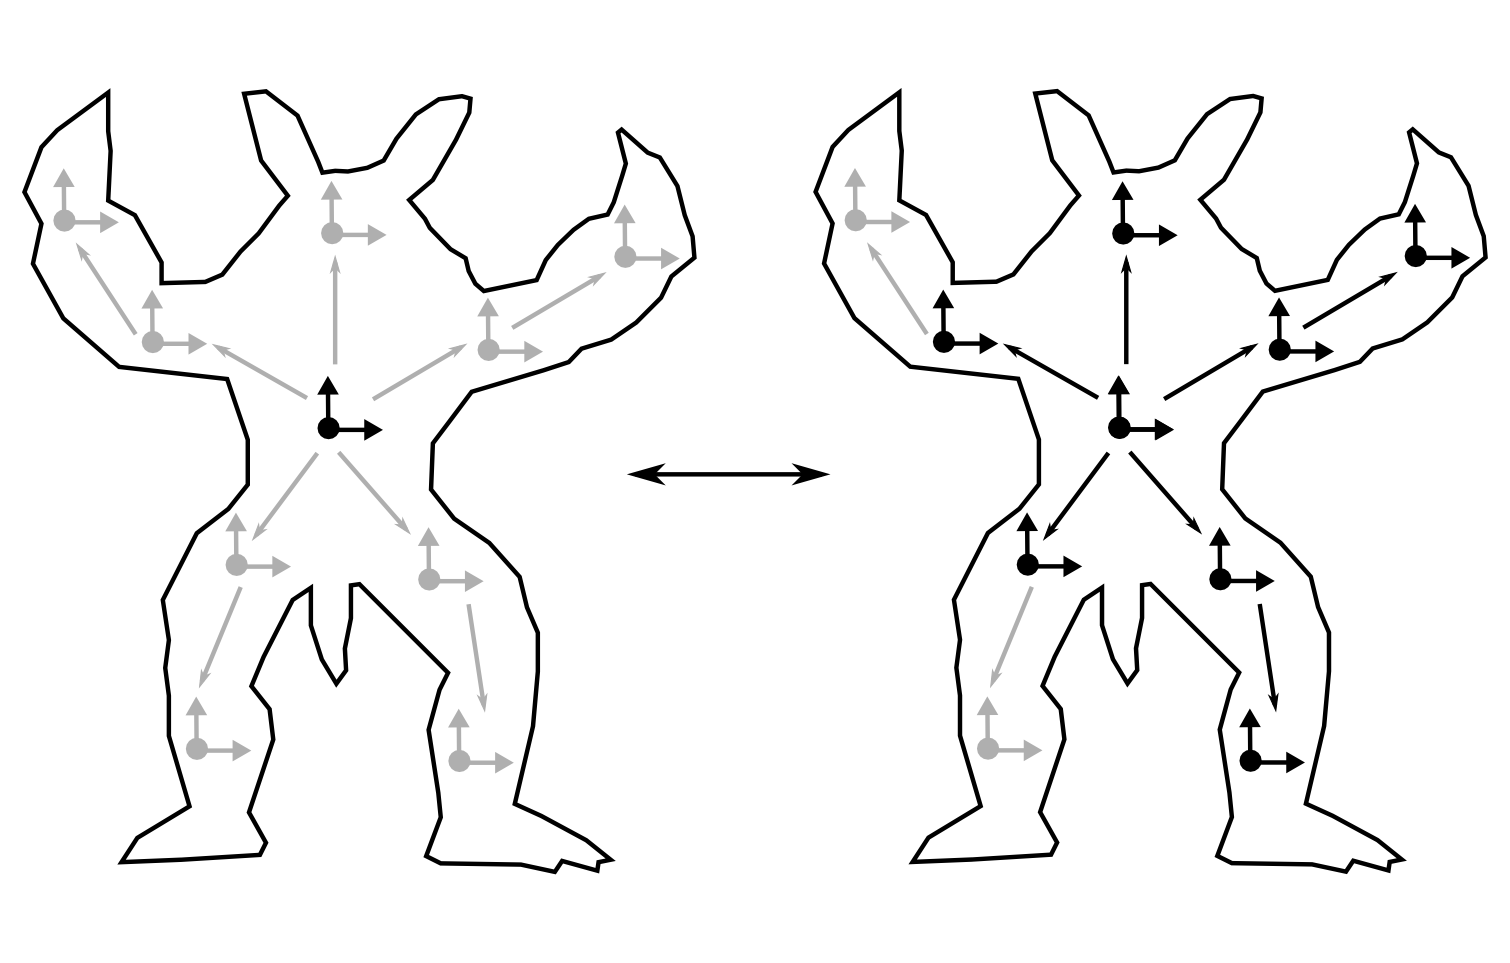
\includegraphics[width=\linewidth]{images/starAdaptivity-cgf2016/particles-hierarchy.png}
		\caption{\label{fig:meshless-hierarchy}}
	\end{subfigure}
	\caption[STAR adaptivity: Meshless techniques]{\label{fig:particleOverview}
		Overview of adaptive meshless techniques.
		(a) Dynamic local re-sampling applies splitting and coalescing operators to degrees of freedom in order to locally refine and coarsen regions of interests (b) Multi-scale methods couple several simulations with different resolutions. Coarser simulations are used as boundary conditions for the finer resolutions. Feedbacks from the finer resolutions are used to avoid divergences between two different resolutions. (c) Hierarchical refinement dynamically activates or deactivates levels of a precomputed hierarchy between degrees of freedom.}
\end{figure}

These different strategies make meshless models particularly useful for material that undergo large irreversible deformations such as the one cited above. However, it is important to keep in mind that the flexibility of meshless models come with expensive nearest-neighbor search algorithms to determine the connectivity between material samples at run time.

We inform the reader that complementary information about SPH adaptive techniques can be found in the state-of-the-art report by Ihmsen et al. \cite{Ihmsen2014:STAR}.

\paragraph*{Dynamic local re-sampling} The idea is to dynamically subdivide or merge particles to fit a desired resolution (see Figure \ref{fig:meshless-operators}). The success of this strategy mainly relies on the re-sampling scheme's ability to ensure stability, to accurately represent boundaries, and to prevent popping artifacts. Depending on the underlying model (SPH, FLIP, MLS) and its sensitivity to intense re-sampling, different strategies have been proposed.
\paragraph*{}
As a full particle-based method, the SPH model is a perfect candidate to dynamic re-sampling. Yet, its sensitivity to particle distribution makes re-sampling strategies challenging. First, the interaction between particles with different sizes increases the error in the pressure term, leading to instabilities. Therefore smooth grading of resolution is required to minimize this error. Second, the change of positions during re-sampling can create a sudden change in density which will result in violent pressure forces, which again lead to instabilities (see Orthmann and Kolb \cite{Orthmann2012}).
Several methods that can be combined were proposed to avoid these local change in density. First, instead of computing the density based on positions, one can use the continuity equation as done by Desbrun and Cani \cite{Desbrun1999}. In order to avoid integration error to be accumulated along the simulation, the density still needs to be re-computed based on positions at a user-defined interval. Then, one can perform position optimization to minimize errors during re-sampling \cite{Adams2007} and use quantity blending over time to smooth out inevitable sampling error \cite{Orthmann2012}.
Also, it is important to keep in mind that another challenge is to efficiently retain the parallel nature of SPH in the adaptive scheme. Zhang et al. \cite{Zhang2008} and Yan et al. \cite{Yan2009} propose two different methods to make splitting and merging operators parallel.
\paragraph*{}
More recently, dynamic re-sampling has been applied to FLIP. As FLIP is a combination of grid and particles, two levels of adaptivity are possible: one on the grid resolution, and the other on the particle sampling. Also, only advection operations are performed on the particles, which results in a less position-sensitive simulation and allows much more flexibility than SPH. More precisely, FLIP does not apply density-based forces to the particles. Consequently, sudden density changes due to particle splitting or merging do not have the same catastrophic consequences as in SPH. However, damping is introduced once particles are merged. This can be taken into account by changing blending parameters of the FLIP simulator as suggested by Ando et al. \cite{Ando2012}.
Early works on adaptive FLIP perform adaptivity only on particles based on a deformability criterion and the distance to surface \cite{Hong2008FLIP, Ando2012}. Ando et al. use the flexibility of FLIP regarding the particles' positions in order to preserve fluid sheets by creating additional particles.
In both methods, the largest particle size is bounded by the cell size of the underlying grid, which precludes aggressive adaptive sampling and the use of a fully adaptive FLIP simulator. Ando et al. \cite{Ando2013} combine an adaptive BCC mesh (see Section \ref{sec:structured}) with adaptive particle sampling to handle highly different resolutions. (see Figure \ref{fig:Ando2013}).
\begin{figure}[!t]
	\centering
	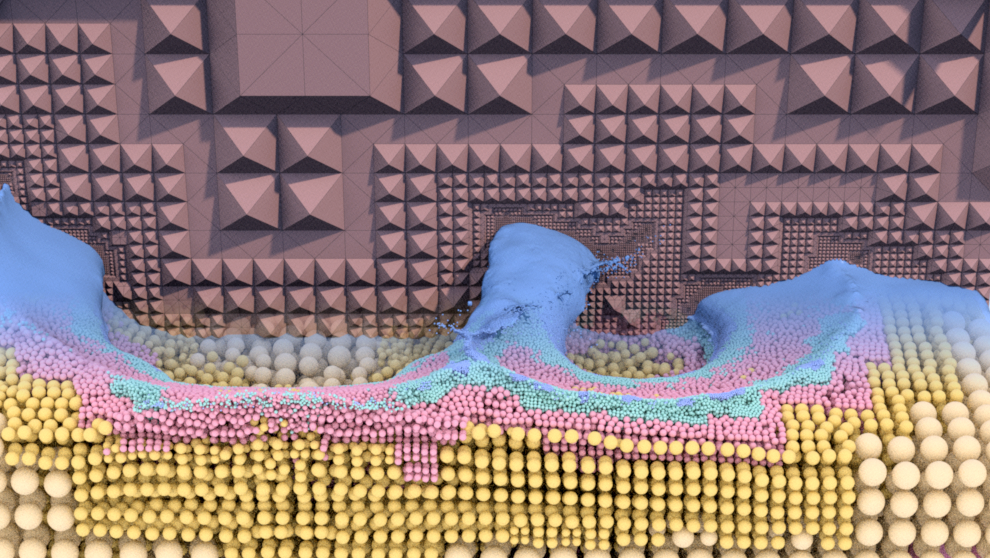
\includegraphics[width=0.8\linewidth]{images/starAdaptivity-cgf2016/Ando2013_3.png}
	\caption[STAR adaptivity: Hybrid refinement of meshes and particles]{Ando et al. \cite{Ando2013} simulate liquid by combining adaptively-sized FLIP particles (bottom, front) with an adaptive tetrahedral mesh for the pressure solve (top, back).}
	\label{fig:Ando2013}
\end{figure}
\paragraph*{}
When simulating solids, local re-sampling is essential in describing phenomena such as large deformations and fracture. First, like mesh-based methods, large deformations create poorly sampled regions leading to ill-conditioned deformation gradients and instabilities. Second, as explained in Section \ref{sec:spatial_refinement}, a challenge in fracture simulation is to reach a sufficiently fine discretization near the tip of the crack in order to obtain a realistic crack path. In these cases, local re-sampling can greatly improve accuracy and stability while retaining efficiency. However, there are two main challenges that require special care.

The first one consists in accurately describing material discontinuities. Most of the time, shape functions are spherical and they must be modified so that sharp boundaries can be represented. In their work on large viscoplastic deformation and fracture, Pauly et al. \cite{Pauly2005} model discontinuities using extended shape functions with transparency criteria, and locally modify a sparse neighborhood graph to update connectivity. Another strategy was proposed by Steinemann et al. \cite{Steinemann2009} to address the high cost of shape functions update. It consists in using a visibility graph to efficiently handle connectivity and approximate material distances used in computing shape functions.

The second one comes from rendering artifacts that can occur at the surface due to splitting. In this context, Jones et al. \cite{Jones:2014:DEF} propose a strategy to re-sample elastoplastic simulation while alleviating popping artifacts. They base their method on the evaluation of each particle neighbor's density. This evaluation is performed using a weighted covariance matrix computed in rest space for each particle $i$, where $\mathbf{u}_{ij}$ denotes the vector between particle $i$ and particle $j$, its neighbor.
\begin{equation}
\label{eq:jones_re-sampling}
\mathbf{B}_{i} = \sum_{j}  \frac{\mathbf{u}_{ij}\mathbf{u}_{ij}^{T}}{\| \mathbf{u}_{ij} \|^{4}}
\end{equation}
If the maximum eigenvalue of $\mathbf{B}_{i}$ is too small, then there are too few particles in the neighborhood and the particle is split in two. New particles are positioned along each side of the eigenvector with the minimum eigenvalue. In order to prevent from rendering artifacts, splittings which are not tangent to the surface are rejected, and particles near the surface are split along the middle eigenvector whose direction is tangent to the surface. Conversely, if the minimum eigenvalue of $\mathbf{B}_{i}$ is too large, then there are too many particles in the neighborhood and the particle is merged with its closest neighbor. The new particle is positioned halfway between the two merged particles.

\paragraph*{Multi-scale methods}
In multi-scale methods, several simulations with different resolutions are coupled in a hierarchical way (see Figure \ref{fig:meshless-multi-scale}).
At the coarsest simulation level $L_{0}$, the whole domain is discretized. Then, each finer simulation level $L_{r}$ discretizes a subset of $L_{r-1}$ with a finer scale. This finer subset is defined to match regions of interests that can be physically or visually motivated. Transitions between two scales are bilateral: the coarsest simulation level $L_{r}$ is used to build boundary conditions for the finer simulation level $L_{r+1}$ and feedbacks from a finer simulation level $L_{r+1}$ to a coarser simulation level $L{r}$ are applied, in order to prevent dynamics of two different levels from diverging. Solenthaler and Gross \cite{Solenthaler2011} and Horvath and Solenthaler \cite{Horvath2013} apply this idea to SPH fluid simulation.
Compared to merging and splitting particles, the main advantage is that interactions between different resolutions are not direct anymore. Thus, stability can be more easily ensured and large differences in resolution can be handled.
In Solenthaler and Gross's approach, a two-scale simulation is performed. High-resolution regions are defined based on the distance to the surface and the view frustum. In these regions, low-resolution particles emit finer particles according to a cubic pattern which ensures a uniform space sampling. Relaxation steps are performed when particles enter the high-resolution region in order to avoid large pressure forces. Horvath and Solenthaler extend the two-scale simulation to multi-scale simulation, and avoid previous artifacts such as mass loss due to particle removal and instabilities due to oversampling near boundaries.

\paragraph*{Hierarchical refinement}
Dynamic re-sampling techniques were also used in frame-based methods to simulate elastic deformations, see \cite{Gilles2011} for a full description of the method. Tournier et al. \cite{Tournier2014} use a hierarchical approach to achieve simplifications during deformation without popping artifacts (see Figure \ref{fig:meshless-hierarchy}). The material is deformed using physically-based control frames organized in a generalized hierarchy. The model can be simplified by attaching frames to their parents at any time in their current relative positions. Activation and deactivation of nodes is performed based on relative velocity and user-specified metrics, while integration points are updated according to the hierarchy. These hierarchical techniques take advantage of their structure to improve efficiency, but may lack of flexibility, especially regarding topological changes.

\subsection{Miscellaneous techniques for spatial adaptivity} \label{sec pr adaptivity}

By far the most popular approach to spatial adaptivity in computer graphics is to add more computational elements where more accuracy or detail is desired, as surveyed in Section \ref{sec:spatial_refinement}. This type of spatial adaptivity is often called \textit{h}-refinement, because the length of an edge in a mesh is typically indicated by the letter $h$. In addition to this tried-and-true strategy, there are other fundamentally different approaches for achieving spatial adaptivity. In the next sections, we will discuss strategies that refine the basis within a single element (a superset of \textit{p}-refinement, which refers specifically to the order of a polynomial basis) and during a subspace simulation, strategies that use multiple grids that move and overlap to track locations where more detail is desired, and strategies that mix different reference frames in order to use the computational degrees of freedom optimally.

\subsubsection{Basis refinement}
\label{sec:basis_refinement}
If we wish to achieve spatial adaptivity without explicitly remeshing (perhaps because it is difficult to control element quality when remeshing, or because a particular application requires that we preserve the original mesh), then we can perform basis refinement instead. The concept of basis refinement can be a difficult one to grasp for newcomers to the field. One of the best ways to understand basis refinement is in the context of finite element methods (FEM). In generic terms, FEM attempts to approximate a function (typically the solution to a partial differential equation) with a very limited, very specific subset of all possible functions. Most methods in computer graphics use linear interpolation within each element, which essentially restricts the solution to a piecewise linear function. For the purposes of this discussion, we would say that the elements are using linear basis functions, and that the overall solution is expressed in a piecewise-linear basis. However, we can actually represent the solution more accurately (in the sense that the solution converges more quickly under refinement) by using more elaborate bases, like piecewise quadratic functions instead of piecewise linear ones.

This section discusses four types of basis refinement: hierarchical basis refinement, polynomial basis refinement, basis enrichment, and adaptive reduced basis functions.
The first three topics discuss adaptivity at the level of basis functions, whereas the fourth is about the adaptive creation of reduced basis in reduced model simulations.

\paragraph*{Hierarchical basis refinement}
In computer graphics, hierarchical basis refinement has mainly been applied to finite element simulations (FEM) of solids and shells \cite{Capell2002,Grinspun2002}. The idea is to refine computational basis functions instead of elements. From a theoretical point of view, there are no differences between hierarchical basis refinement and hierarchical element refinement. Both adaptively add more degrees of freedom with increasingly local support in order to improve accuracy where needed. Both use hierarchical schemes in order to efficiently sample the simulation domain.
The main differences are practical. By refining basis functions instead of elements, compatibility between regions with different resolutions are implicitly handled.
This makes adaptivity much easier and general.

For instance, hierarchical basis refinement allows a simple handling of \emph{T-junctions}.
In FEM, each element's node carries a basis and builds a local stiffness matrix from its node's stiffness which are then assemble into a global stiffness matrix.
During this process, only independent degrees of freedom should add their contribution to the global matrix. However, when using hierarchical element refinement, non-independent degrees of freedom are added during the subdivision of the simulation mesh. They are called \emph{T-junctions} or \emph{T-nodes} (see Figure \ref{fig:tjunctions}) and require specific handling. Suddenly, a simple subdivision scheme becomes dependent on the dimensionality, the element type and the basis order, thus requiring important implementation work. In contrast, hierarchical basis refinement handles \emph{T-nodes} at the basis level by making sure that no bases are redundant. The hierarchical structure makes this process simple and thus offers a more general framework for adaptivity which can handle arbitrary resolution differences.
\begin{figure}[!h]
	\centering
	\begin{tabular}{cc}
		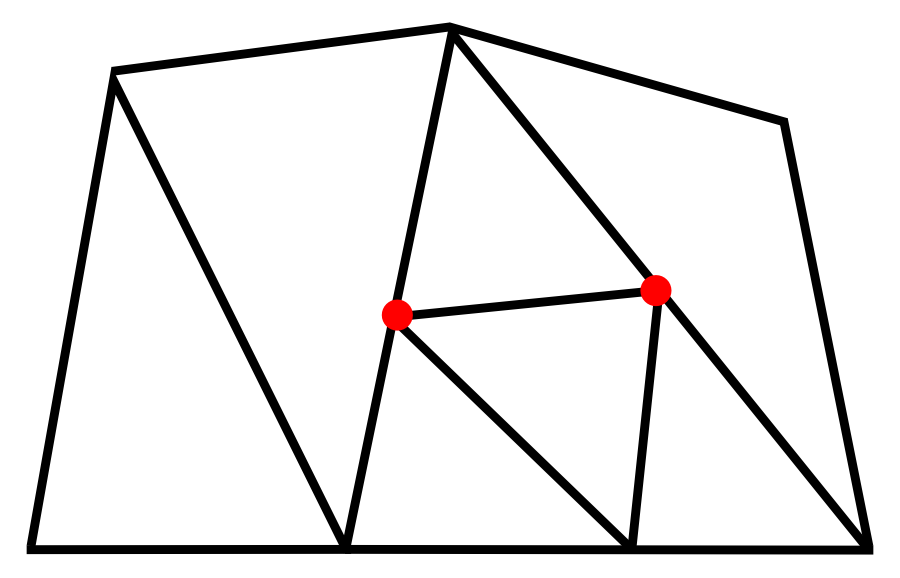
\includegraphics[width=0.35\linewidth]{images/starAdaptivity-cgf2016/tjunction-triangle.png} &
		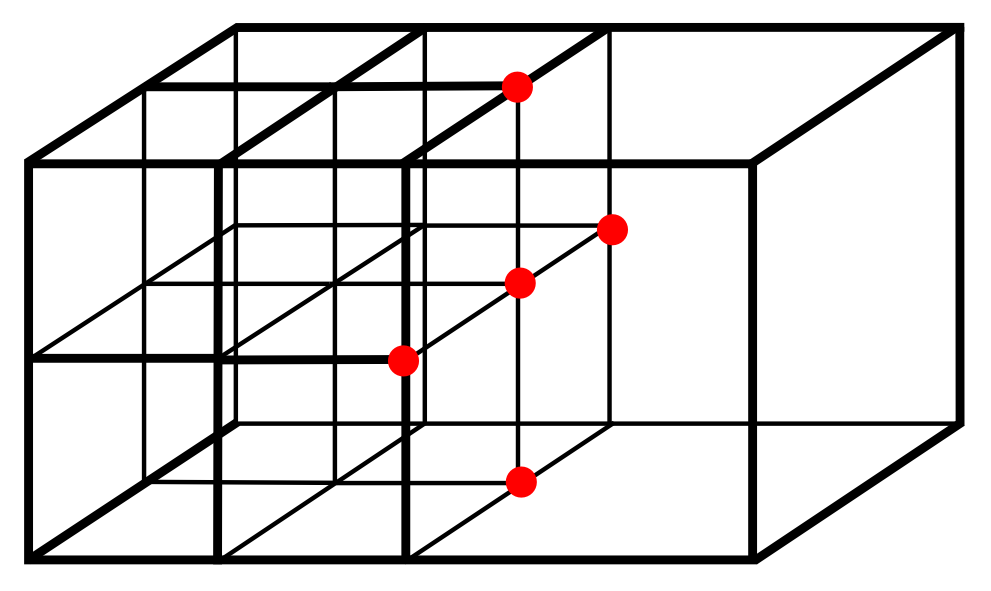
\includegraphics[width=0.35\linewidth]{images/starAdaptivity-cgf2016/tjunction-grid.png} \\
		(a) & (b)
	\end{tabular}
	\caption[STAR adaptivity: T-junction]{\label{fig:tjunctions} Refinement by element subdivision is attractive by its simplicity for 2D and 3D meshes, however it introduces T-junctions (in red) at interface between resolutions with different sizes. Bookkeeping or extra-remeshing operations are required to take care of these non-independent degrees of freedom.}
\end{figure}

Capell et al. \cite{Capell2002} embed a high-resolution mesh in a hexahedral complex and precompute a hierarchy of bases up to a given level of refinement. During the simulation, depending on the amount of deformation, each level of the hierarchy will refine or coarsen, thus updating the current set of active bases. Basically, it is the same idea of \cite{Debunne2001} but from a basis point of view.

The Conforming Hierarchical Adaptive Refinement Methods (CHARMS) framework of Grinspun et al. \cite{Grinspun2002} generalizes the idea of spatially refining the bases instead of the elements. They provide an in-depth explanation of the concept and describe numerous results of basis refinement applied to shells, solids and electrocardiography simulations.
In fact, it is quite surprising that this method was not more studied or extended in the last decade. A possible explanation is the fact that, in the last few years, adaptivity proved to be essential for large and complex deformations such as visco-elastic, visco-plastic flows. In those cases, hierarchical refinement is not sufficient anymore to ensure well-conditioning of the system matrices. 

\paragraph*{Polynomial basis refinement}
Polynomial basis refinement methods, also called \emph{p-adaptivity}, increase or decrease the order of the basis functions.
For a given spatial resolution, this allows to improve the quality of the deformation without remeshing. In computer graphics, using high order approximation to resolve fine details is not new. However mixing different orders of approximation to adaptively resolve details was only recently applied in the context of fluid simulation and elastic deformations.

For fluid simulation, the smoothness of velocity and pressure makes \emph{p-adaptivity} potentially much more efficient than geometric adaptivity, because the error per degree of freedom decreases exponentially with the approximation order but only geometrically with the spatial resolution. In this favorable context, Edwards and Bridson \cite{Edwards2012,Edwards2014} use polynomial basis refinement in a Discontinuous Galerkin FEM framework in order to simulate detailed water with coarse grids. They use low-order bases deep inside the liquid and increase the basis order closer to the liquid surface, where more visual detail is desired (see Figure \ref{fig:pfluid}). By using basis refinement instead of element refinement, they can keep the simple structure of a low resolution Cartesian grid while pushing back the limit on the scale of details in one cell. In terms of cost, their method is approximately as expensive as a classical high spatial resolution simulation but it provides much more details such as extremely thin sheets.
\begin{figure}[t]
	\centering
	\begin{subfigure}[!ht]{0.48\linewidth}
		\centering
		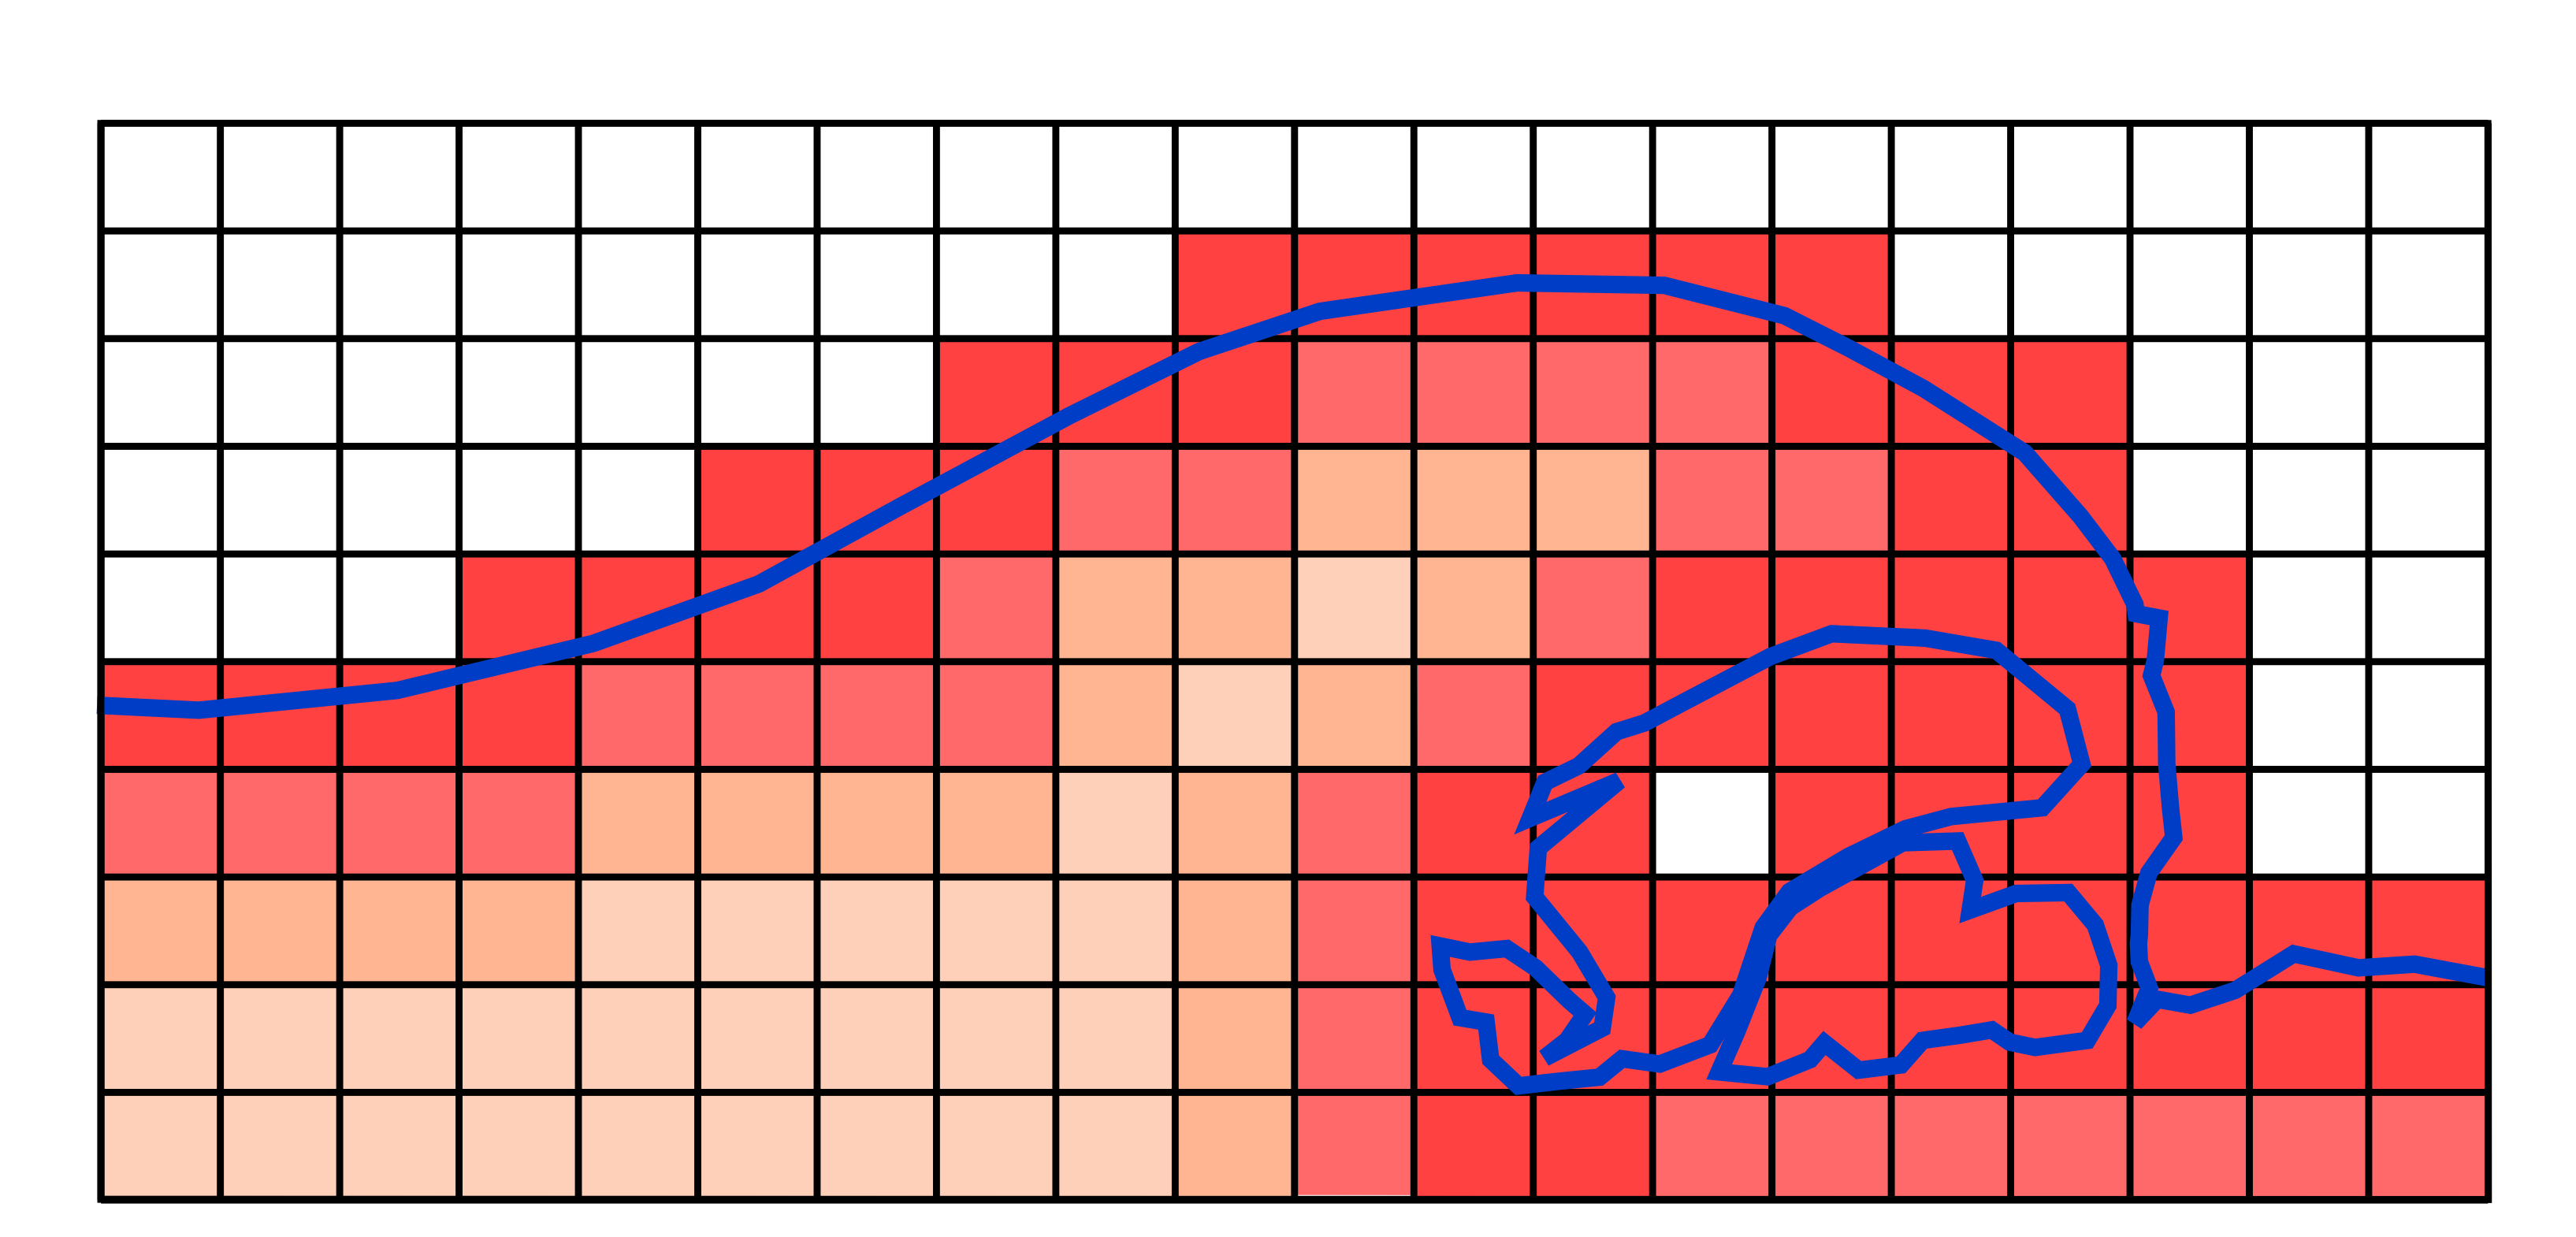
\includegraphics[width=\linewidth]{images/starAdaptivity-cgf2016/pfluid.png}
		\caption{\label{fig:pfluid}}
	\end{subfigure}
	\hfill
	\begin{subfigure}[!ht]{0.48\linewidth}
		\centering
		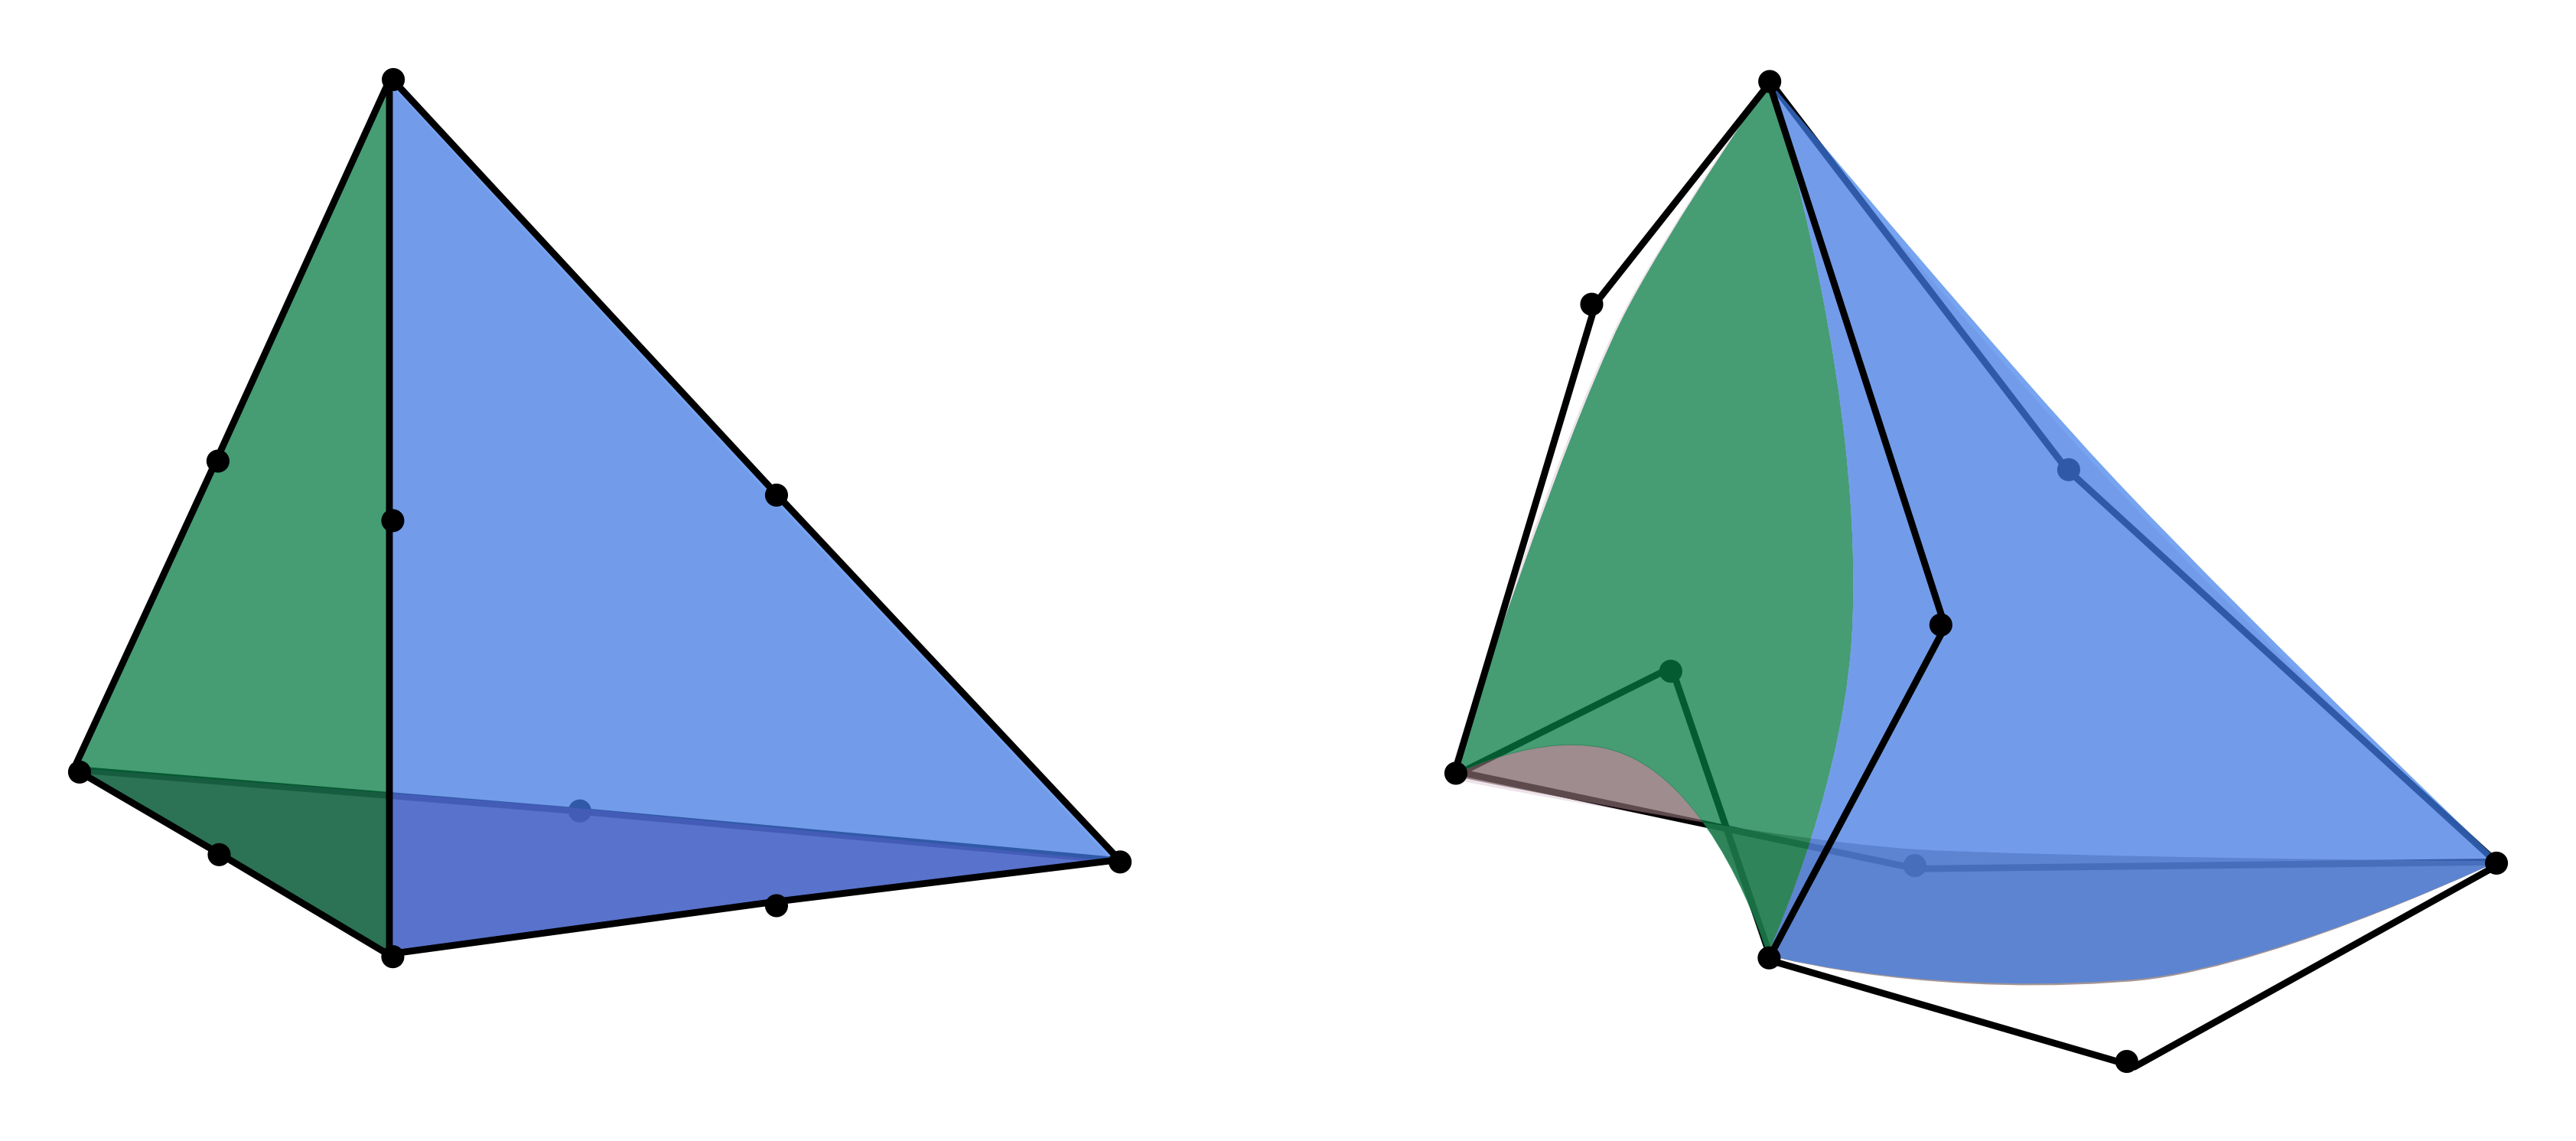
\includegraphics[width=\linewidth]{images/starAdaptivity-cgf2016/quadratic.png}
		\caption{\label{fig:quadratic_fem}}
	\end{subfigure}
	\caption[STAR adaptivity: p-adaptive techniques]{\label{fig:padaptivity}
		Illustrations of p-adaptive techniques for (a) fluids and (b) deformable solids.
		In (a) Each fluid cell uses a different approximation space depending on its distance to surface (blue line). Surface cells (in red) use fourth order polynomial to precisely approximate pressure. A smooth grading of the approximation is performed inside the fluid (lighter cells) that allows to save computational time.
		In (b) the canonical tetrahedron with quadratic control points and next to it the quadratic deformation induced by the deformed control mesh. Such a deformation would require many linear elements.
	}
\end{figure}

Bargteil and Cohen \cite{bargteil2014animation} animate deformable bodies by combining linear and quadratic B{\'e}zier elements.
The main advantage of their method is the ability to locally increase degrees of freedom and to simulate nonlinear geometry without remeshing (see Figure \ref{fig:quadratic_fem}).
To decide whether an element should be linear or quadratic, they compare the linear and quadratic predicted positions of the midpoint of each edge of the element. If the difference between the two positions is larger than a threshold then the edge becomes quadratic. If the difference is less than another threshold then it becomes linear. Thus, some elements can have linear and quadratic edges, usually in transition regions. Bargteil and Cohen observe that, as the number of degrees of freedom increases, visual differences between linear and quadratic elements become difficult to discern. Moreover, the additional cost remains important and local deformations on the surface of a quadratic element due to collisions still cannot be resolved without element refinement. Therefore, their method is particularly efficient on low-resolution models, where it provides smoother geometry and better dynamics quality.

In both cases, the differences of resolution between two regions that can be achieved only using \emph{p-adaptivity} are limited. An important avenue for research would be to combine those methods with geometric adaptive techniques. Such methods have been well studied in engineering fields and are called \emph{hp-adaptive} methods.

\paragraph*{Basis enrichment}

Another way to add spatial detail to a physical model without remeshing is by using ``basis enrichment.'' The main idea behind basis enrichment is to adaptively add carefully-chosen basis functions that are specifically designed for the phenomena being modeled. (This is in contrast to p-refinement, which is restricted to polynomial functions, regardless of the phenomena being simulated.) For an example of basis refinement, consider an object is being fractured; some material that used to be connected together will have to be split in two. A simple linear basis function could be split into two functions that are linear on one side of the fracture and zero on the other, as illustrated in Figure \ref{fig:basisenrichment}. 
\begin{figure}[t]
	\centering
	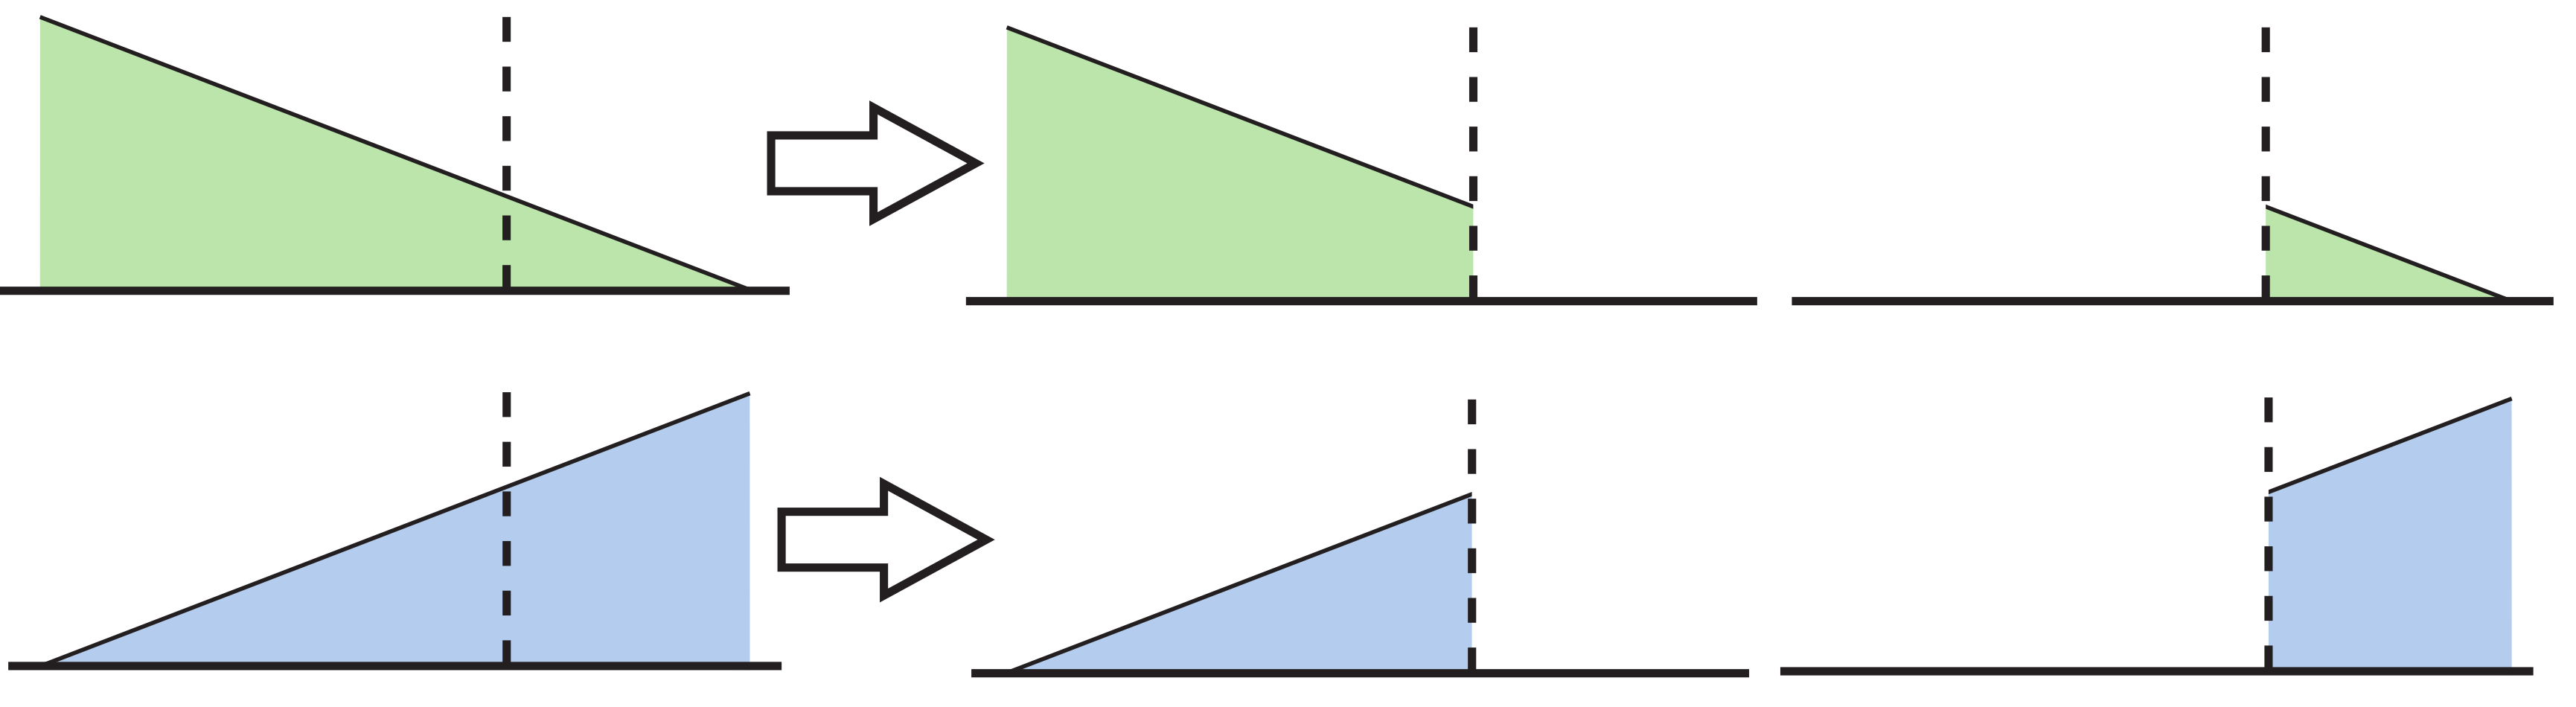
\includegraphics[width=0.8\linewidth]{images/starAdaptivity-cgf2016/xfem.png}
	\caption[STAR adaptivity: XFEM illustration]{\label{fig:basisenrichment}
		A one-dimensional element with linear basis functions can simulate a fracture by enriching its basis. Here, the new basis functions drop off to zero on the other side of the fracture site indicated by the dashed line, directly encoding the severed connection.
	}
\end{figure}

This type of basis replacement effectively avoids remeshing by inserting a fracture directly into the basis itself. Note that in this case, we opted to enrich the basis with these particular ``step'' functions which drop to zero after a certain point, instead of trying to fit some polynomial that might overshoot or otherwise imperfectly capture the desired physics. Such basis enrichment techniques have been termed the ``general finite element method'' (GFEM) or ``extended finite element method'' (XFEM) \cite{belytschko2009review}.

Adaptive basis enrichment methods have been recently applied in many computer graphics contexts.
The virtual node algorithm uses basis enrichment to stabilize fracture and cutting simulations~\cite{Molino2004,hegemann2013level}. Instead of remeshing and potentially inserting poorly-conditioned elements, the virtual node algorithm essentially copies the entire element and adapts its basis functions to the fracture site. The virtual node algorithm  has recently been improved to robustly allow multiple cuts in a single element \cite{Sifakis2007:Cutting,Wang2014}. One drawback to adaptive basis enrichment is that complicated cuts can require arbitrarily complicated basis functions that may not be simple to compute. In the case of cutting thin shells, Kaufmann and colleagues~\cite{Kaufmann2009} note that the most physically-appropriate enrichment functions require the solution of a Laplace equation with time-varying boundary conditions. Similar basis enrichment techniques may not be computationally feasible for the adaptive simulation of more complicated volumetric phenomena.

\paragraph*{Adaptive reduced bases}
As pointed out by Bargteil and Cohen \cite{bargteil2014animation}, volumetric elastic effects are usually low-resolution in space, because we often care about longer time scales in computer graphics.
Model reduction methods, also called subspace simulation, exploit this fact to turn extremely costly nonlinear finite element simulations into interactive ones.
The idea is to solve equations of motion in a reduced basis that is usually computed using modal analysis or from a database using principal component analysis (PCA).
Thus, instead of having a complexity dependent on the simulation mesh resolution, it only depends on the size of the reduced basis (the number of deformation modes) which is typically much smaller.
A cubature scheme is used to perform integration on only a reduced sets of well-chosen samples. In the end, this allows simulation of nonlinear deformable models with orders of magnitude speed-up.

The drawbacks are that the creation of the basis requires heavy precomputation, and that the motion of the model is constrained to lie in this basis. Furthermore, while the full finite element simulations often have local compact basis functions and sparse system matrices (because each degree of freedom is a vertex that only influences its neighbors locally), reduced simulations tend to have global basis functions and dense system matrices (because each degree of freedom impacts all points in space simultaneously). Small dense systems are often more efficient than large sparse ones, but the increased storage requirement limits how many modes can be feasibly included in model-reduced simulations, and it limits the use of model reduction in settings where large numbers of modes are essential for visually-plausible behavior (like cloth and fluids).
Therefore model reduction is only truly efficient for smooth global deformations and predictable scenarios where it is possible to build a basis that remains constant over time. It is also only useful in situations where a limited number of modes can adequately describe the system.

Several strategies have been proposed to overcome some of these drawbacks by adaptively improving the reduced basis. Common components to those strategies are the different processes to update the basis and the criteria used to decide when the basis should be adapted. Moreover, a common challenge is to ensure temporal coherence while adapting the basis.
Kim and James \cite{Kim2009Skipping} combine a full nonlinear simulation with subspace simulation in order to exploit coherence in the global motion of the model.
They incrementally build a reduced-order nonlinear deformable model as the full nonlinear simulation progresses. When possible, full nonlinear steps are skipped with subspace steps resulting in significantly cheaper steps. The challenge of this strategy is to provide efficient operators to update the reduced-basis and to robustly choose which steps can be reduced. We briefly describe the two main operations that compose the incremental construction of the basis: the updating operation and the downdating operation. The updating operation adds a new vector to the basis only if it is significant. To do so, a displacement vector received from a full simulation step is orthogonalized against the existing basis. If its norm is above a given threshold then it is concatenated to the basis. The downdating operator is applied when the basis reached its maximal size $r$ and a new significant vector needs to be added. The basis is then modified so that the $r/2$ most significant directions are preserved. Finally, as the cubature (reduced integration) is dependent on the basis, it also needs to be updated. The updating operation is triggered through different criteria depending on the application. Kim and James describe criteria for quasi-static and dynamic simulations. The dynamic case is particularly challenging as the error is history dependent, which means that taking full steps after reduced steps do not correct errors from the subspace simulation. This method presents impressive speed up for nonlinear simulations. However, the performance is highly dependent of the rate of expansion of the basis.

As subspace simulation tends to reproduce the global motion of an object, it is particularly challenging to produce very local deformations in this framework. A direct consequence is a simplification of the dynamic behavior. Harmon and Zorin \cite{Harmon2013} tackle this problem by including \textit{a priori} knowledge in the building of the basis. More precisely, they augment a standard precomputed basis with a dynamic basis. This dynamic basis is built with custom functions derived from analytic solutions to static load. Unpredictable local deformations that arise due to collisions and contacts can then be handled. Moreover, as the change in the basis is very local, they can ensure temporal coherence by projecting the current subspace coordinate vector into the new basis whenever it changes. However, a limitation of the addition of local modes is a restriction on the time step size in order to properly represent the dynamics. Furthermore, the size of local displacements is limited.
\\
Pushing further the idea of using \textit{a priori} knowledge in the building of a reduced basis, Hahn et al. \cite{Hahn2014} perform adaptive subspace simulation of cloth. They start with a large amount of high-resolution simulation data from multiple training animations, and convert it into a database of low-dimensional bases associated with poses. Then at each time step, they adaptively choose a subset of low-dimensional bases in the data base depending on the pose of a clothed character.
Highly nonlinear folds and wrinkles, which typically are very hard problems for subspace simulation, can then be reproduced. Dynamics is damped near tightly constrained regions such as sleeves, but this may be acceptable in practice for animating tight clothing.

Recently, Teng et al. \cite{Teng2015} propose the use of subspace condensation to locally switch between subspace and fullspace simulation at run time. When dealing with localized deformations, this allows the behavior not to be limited by \textit{a priori} knowledge such as in \cite{Harmon2013} and \cite{Hahn2014}.

\subsubsection{Moving grids}
\label{sec:movingMesh}
As mentioned in Section (\ref{sec:structured}), grids are an efficient and simple data structure compared to unstructured meshes. However, this simplicity is counterbalanced by a severe lack of flexibility. Firstly, simulating fluids on very large domains requires a prohibitive amount of memory. Secondly, focusing computational resources on regions of interest remains a challenge.
While octrees and other adaptive structured meshes discussed in Section \ref{sec:structured} address these challenges, they lose the cache-coherent structure that makes uniform grids so efficient.
Moving grids methods, also called Chimera grids, allow more flexibility while keeping the advantages of Cartesian grids. The main idea is to use one or more computational grids and allow them to move at each time step to follow the region(s) of interest.

Shah et al. \cite{Shah2004} propose a simple approach in which a single grid is used whose location and size changes to enclose the region containing significant flow.
This strategy is useful when there is only a single region of interest in the fluid, such as when simulating explosions.

A more versatile approach is to use multiple independently moving grids, typically centered at each moving object in the scene.
The grids may undergo pure translation \cite{Cohen2010}, or may also rotate with the object \cite{Dobashi2008:adaptiveGrid,English2013}; in the latter case, centrifugal and Coriolis forces may also need to be taken into account.
A coarser background grid can also be used to represent the global flow in the remainder of the domain not covered by any local grid.
The major question that arises in these approaches is how to couple the degrees of freedom in regions where two or more grids overlap.

For interactive smoke simulation, Cohen et al.~\cite{Cohen2010} omit the coupling step entirely.
Instead, smoke particles that lie within multiple overlapping grids are simply advected with a weighted average of the flow velocities indicated by different grids.
The resulting motion is not physically valid, but works well for interactive applications.

To perform correct coupling for globally incompressible flow, there are two possible strategies: solve for incompressibility as usual in each grid and transfer data between them in an outer loop, or build a single discretization that couples all the grids together.
Dobashi et al.~\cite{Dobashi2008:adaptiveGrid} use the former approach to efficiently simulate interaction between smoke and rigid objects. Pressure is solved using a modified Gauss-Seidel solver where each iteration follows three steps.
First, data from coarser grids is copied to the boundary cells of finer grids for use as boundary conditions.
Then, pressure is computed independently on each grid.
Finally, data from the interior cells of finer grids is copied to overlapping coarser grids.
This process is repeated until it converges; unfortunately, convergence can be slow.
More recently, English et al.~\cite{English2013} developed a full moving Cartesian grids model.
Instead of solving for pressure on each grid separately, they combine all grids in a single discretization.
Coarse grid cells that contain the cell center of a finer cell are removed, and a Voronoi mesh is built using the remaining cell centers.
An monolithic Poisson solver then computes the pressure over the entire mesh.

In summary, moving grids are a good solution for accelerating Eulerian fluid simulation. In the applied math vocabulary, they belong to dynamic domain decomposition methods.
These methods tackle with success the challenge of increasing the local accuracy of Cartesian grids methods while keeping their natural efficiency. However, while such methods are extremely efficient for environments where regions of interests are known or easy to compute, they are not well suited for interactive scenarios where any number of new regions of interest may pop up at any location and time, and where adaptive particle simulation remain more appropriate.

\subsubsection{Mixed models}
\label{sec:mixed-models}

Another important strategy for adaptively focusing computation in computer animation is to selectively apply a mixture of different computational models. The motivation is that every model has its own strengths and weaknesses, and some are better suited to some situations than others. In particular, many methods combine Eulerian reference frames (which describe motions relative to a fixed point in space) with Lagrangian reference frames (which describe motions relative to a physically important moving trajectory). The driving goal is to judiciously combine techniques in a way that leverages the strengths of each model and suffers none of the drawbacks.

While most of these mixed models represent a clever combination of techniques whose whole is greater than the sum of its parts, the mixed models which could not be classified as ``adaptive'' have been omitted from this work. This section only discusses mixed models that adaptively change from one model to another when the situation calls for it.
This section is separated into methods used to simulate solid objects and methods used to simulate fluids.

We note that numerous other techniques use two-way coupling between different phenomena (\hspace{1sp}\cite{carlson2004rigid,robinson2008two,shinar2008two,Remillard2013}, to name a few). However, while these approaches are adaptive in the sense that they modify computation depending on the phenomena being simulated, we feel these two-way coupling methods are outside of the scope of this section. Instead of surveying all possible combinations of different phenomena-specific discretizations, we only discuss here methods that combine different discretizations of the {\em same phenomena} in order to gain a computational speedup.

\paragraph{Solids}
While most mixed models for simulating solid dynamics do not quite adapt their models to their environment, both Sueda et al. \cite{Sueda2011} and Servin et al. \cite{Servin2011} successfully address the challenging problem of simulating stiff elastic strands in a collision-heavy scenario. They accomplished this by introducing Eulerian nodes into a largely Lagrangian strand simulation. The Eulerian nodes sit still at important contact points, while the standard Lagrangian nodes sample the strands as normal. These models are ``adaptive'' under our definition, because the Eulerian nodes add local detail and their location is decided during run-time.


\paragraph{Fluids}
The large memory and computation requirements of 3D fluid discretizations are undesirable, so 2D simplifications are often preferred when applicable. In addition, an Eulerian reference frame is popular for guaranteeing a uniform mesh-spacing, maintaining cache-coherence, avoiding remeshing, and describing swirling flows without explicitly sampling complicated trajectories. However, Eulerian methods are often inferior to their Lagrangian counterparts when sampling fine individual features like droplets and bubbles, or for explicitly tracking many individual vortices.

This section describes many techniques that adaptively combine 2D/3D and Eulerian/Lagrangian techniques in order to get the most out of a fluid simulation. We first survey various methods that combine Eulerian techniques with Lagrangian particles (droplets, bubbles, vortices, etc.). Next, we discuss how some Eulerian models also use Lagrangian particles to couple directly with SPH solvers. After that, we review some methods which combine 3D solvers with 2D techniques or with surface physics.

\subparagraph*{Eulerian simulation \& Lagrangian particles}

Several early methods combined Eulerian fluid simulations with Lagrangian particles to animate splashing droplets. O'Brien and Hodgins \cite{OBrien1995} combine a 2D pipe-based fluid model with particle-based droplets. Holmberg and W\"unsche \cite{Holmberg2004} create an Eulerian waterfall model and used Lagrangian particles to animate spray, and Kim et al. \cite{Kim2006:Splash} used particles from a 3D surface tracker to fill in missing splash details. Chentanez and M\"uller \cite{Chentanez2010} combine an Eulerian discretization of the shallow water equations with a Lagrangian simulation of spray, splash, and foam particles. The particles add important missing details to the simulations and are allocated dynamically at run-time.

Researchers also use Lagrangian particles to capture bubble behavior in Eulerian simulations. Mould and Yang \cite{Mould1997} augment a height-field model with Lagrangian particles for droplets and bubbles. Many simulation methods \cite{Greenwood:2004:BBE:1028523.1028562,Hong2008Bubbles,Patkar2013} compute a 3D Eulerian fluid simulation, and they represent bubbles that are too small to be resolved on the grid with Lagrangian particles. The differences in these methods lie in the varying bubble dynamics and the subtleties of how to transition between the Eulerian grid bubbles and the Lagrangian particle bubbles.

The main concept for these methods is to use an Eulerian representation for the bulk of the flow, but to adaptively turn to a Lagrangian particle representation whenever the Eulerian model is insufficient. This switching point is often easy to detect, because it occurs exactly when the diameter of a water droplet or bubble falls below the Eulerian grid resolution. Not only does this strategy conserve mass and momentum better than simply deleting small features, but it fills in visually important information by animating sprays as a collection of small Lagrangian droplets and foams as a collection of Lagrangian bubbles. Lagrangian droplets and bubbles are practically indispensable in a production workflow, because the small expense of adding additional point geometry with simple physics pays off with enhanced visual realism.

\subparagraph*{Eulerian simulation \& SPH}
Eulerian methods can also be combined with Lagrangian particles in other ways beyond droplets and bubbles.
Losasso et al. \cite{Losasso2008} combine SPH with a FLIP simulation, Wang et al. \cite{Wang2013} combine SPH with a Lattice-Boltzmann simulation and Chentanez et al. \cite{Chentanez2014} combine SPH with 3D Eulerian grid.
This idea of adaptively switching between Eulerian simulations and SPH is still an active research topic. Using SPH instead of simple passive or ballistic particles is clearly more realistic, but it comes with the expense of additional neighborhood operations and more delicate numerical calculations in general. It is not clear yet whether the realism gained by augmenting an Eulerian simulation with SPH particles is worth the computational expense.

\subparagraph*{Combining 2D \& 3D}
Several techniques like discretizing the shallow water equations~\cite{layton2002numerically,hagen2005visual} or linearized wave equations~\cite{kass1990rapid,tessendorf2004interactive,keeler2014ocean} are useful for reducing computational degrees of freedom, but we do not believe they are inherently {\em adaptive} by themselves, and we do not discuss them in detail in this document. However, several techniques utilize these 2D discretizations in ways that we would classify as an adaptive ``mixed-model'' approach.

The work of Th\"urey et al. \cite{Thurey2006:Coupling} combines a 3D Lattice-Boltzmann simulation with a 2D simulation of the shallow water equations, allowing a local region that to adapt to 3D phenomena while distant motion remains a simple height field. Chentanez et al. \cite{Chentanez2014} combine a 3D Eulerian solver with both a 2D shallow water solver and a particle-based fluid simulation. Mixing three models allows them to simulate extremely detailed water interactions at efficient frame rates. These methods fit our definition of adaptivity, because they both locally increase the computational degrees of freedom in interesting regions, and these decisions of where to place the new degrees of freedom are decided at run-time as the simulation progresses. As these papers suggest, adaptively switching simulation dimensions will clearly make animations more efficient, because the computational complexity plummets as the simulation transitions from 3D to 2D. The only reservations here are that there is a significant implementation expense to maintaining two or more solvers (one for each dimension), and the seamless coupling between dimensions is a sensitive process that is still being actively researched.

\subsection{Discussion} \label{sec conclusion}
Adaptive physically-based models are becoming ubiquitous in computer graphics.
In the last decade, various techniques for almost all types of deformable models have been proposed and extended.
In this section, we have classified adaptive techniques into five different categories: (1) temporal adaptivity, (2) geometric adaptivity, (3) basis refinement, (4) moving grids and (5) mixed models.
For each category, we have described the variants that were developed for different applications and have discussed their strengths and weaknesses.

Among those different categories, geometric adaptive techniques are the most studied, and are perhaps the most intuitive due to their geometrical nature.
The many variations in application contexts such as dimensionality and discretization have led to a proliferation of different innovative techniques.
Yet, as we have tried to show, there are also many commonalities between aspects of disparate techniques, for example in terms of refinement criteria, and there is potential for consolidation of the many approaches in this area.

In the opposite direction, mixed models represent an important area of work.
Unfortunately, as they rely on the specific characteristics of each model, it is more difficult to extract general patterns and strategies. 
Even so, they perfectly represent the idea and the versatility of adaptive techniques by combining the strengths of different approaches as the simulation evolves.

For now, polynomial basis refinement represents only a small fraction of the methods studied. In computer graphics, this is a very recent topic, but which can build on strong foundations from engineering and applied mathematics where it has been extensively studied. Results in solid and fluid simulation show that polynomial basis refinement can indeed produce impressive animations. One of the most exciting avenues of future research is the combination of this technique with geometric adaptivity.

In subspace simulation, adaptive reduced bases can greatly extend the range of deformation that can be achieved by introducing local and non-linear deformations such as wrinkles. Nevertheless, there is still a large room for improvement and innovation, especially regarding the possibility to handle topological changes and couple different subspace simulations such as deformable solids and fluids.

Even if there are only a few works that focus on temporal adaptivity, these methods are widely used and play a crucial role in ensuring stability and efficiency. Their importance is due to two main reasons. First, spatial and temporal resolution are often strongly related. Secondly, the necessary temporal resolution is inherently dependent on the events occurring during a simulation and cannot always be predicted in advance, necessitating adaptive techniques. As we seek to resolve details at increasingly finer time scales, further research will be required to capture them without paying an exorbitant computational cost.

Adaptive methods are not without limitations, and we briefly summarize the major ones.
At present, setting up a new adaptive method is quite difficult: adaptive methods have often been application-specific so far, which makes the study of existing solutions quite intricate. Adaptivity usually makes the implementation of a model much more complex and may ruin the regularity of computations, causing incompatibilities with GPU implementations. Evaluating the future overhead due to the online adaptation process is often difficult, which may make such techniques unusable in performance-constrained contexts such as interactive applications.
There are also potential concerns relating to simulation fidelity. If not tackled with care, popping between different spatial and temporal resolutions may cause instabilities and visual artifacts. Furthermore, the energy diffusion that necessarily occurs when permanently adapting a model may be an issue when an accurate simulation is required.

Nevertheless, the space of adaptive simulation techniques is vast and fruitful, and many compelling benefits have been uncovered so far.
There is much room for future work in developing new adaptive methods which are both easier to implement and still generic enough to be used in different applications. This challenge requires methods which, for example, minimize the overhead due to additional structures while making it possible to integrate different adaptation criteria.
Many other avenues of future research remain, including combinations of different forms of adaptivity and techniques that adapt between different dimensionalities, different formulations, and other characteristics that have traditionally remained separate.

\subsection{Conclusion on adaptive physically-based models}
Adaptive methods allow to make physics-based simulation efficient by focusing the computational resources where and when needed. 
This made possible to interactively run complex simulations and to resolve complex behaviors which require a very fine scale.
However, controlling a physics-based model remains a tedious task. 
It usually consists in tweaking parameters whose understanding require advanced knowledge of the underlying model. 
In the end, the user apply a trial-and-error process to find the parameters which produce a result close enough to its expectations.
In the following section, we present different methods for the control of physics-based animation.

\section{Control of physics-based animation}
\label{sec:starSimulationControl}

As we mentioned in the introduction, computer were used for producing animations in two main ways. 
First, principles of traditional animation were adopted, leaving the animator to describe the key-frames that would bring life and style to characters. 
Second, physics was used to animate objects whose complexity in terms of scale and behavior would have been intractable for a single animator. 
Nowadays, these two use cases are only the extremities of a large spectrum. 
In between lies the control of physics-based animations which tends to take into account both user directions, that will bring life and style, and physics, that will handle the exciting complexity and dynamics of the physical behavior.
In this section, we illustrate the problem of simulation control and describe the main solutions proposed so far.
\subsection{Problem: The trials and errors process}
How to control a physics-based animation is an old problem in Computer Graphics. In order to understand the different problems that arise, it is good to start from the most naive way of controlling a physics-based animation: trials and errors. 

Let's say we have to design an animation of a ball launched on the ground that bounces two times before hitting the center of a target on the ground. 
The elastic behavior of the ball and the changes of speed make it a hard animation for a key-framing animator. 
Using physically-based simulation methods, the behavior takes some time to compute but can be easily solved.
As the simulation is an initial value problem, the whole behavior of the ball is dictated by the initial and boundary conditions of the simulation, the material parameters of the ball and the external forces that can be set to help guiding the animation. 
The trials and errors process consists in setting these conditions and parameters, running the simulation and correcting the parameters until the ball reaches the desired target (see Figure~\ref{fig:trialErrorProcess}). 
\begin{figure}[!h]
	\centering
	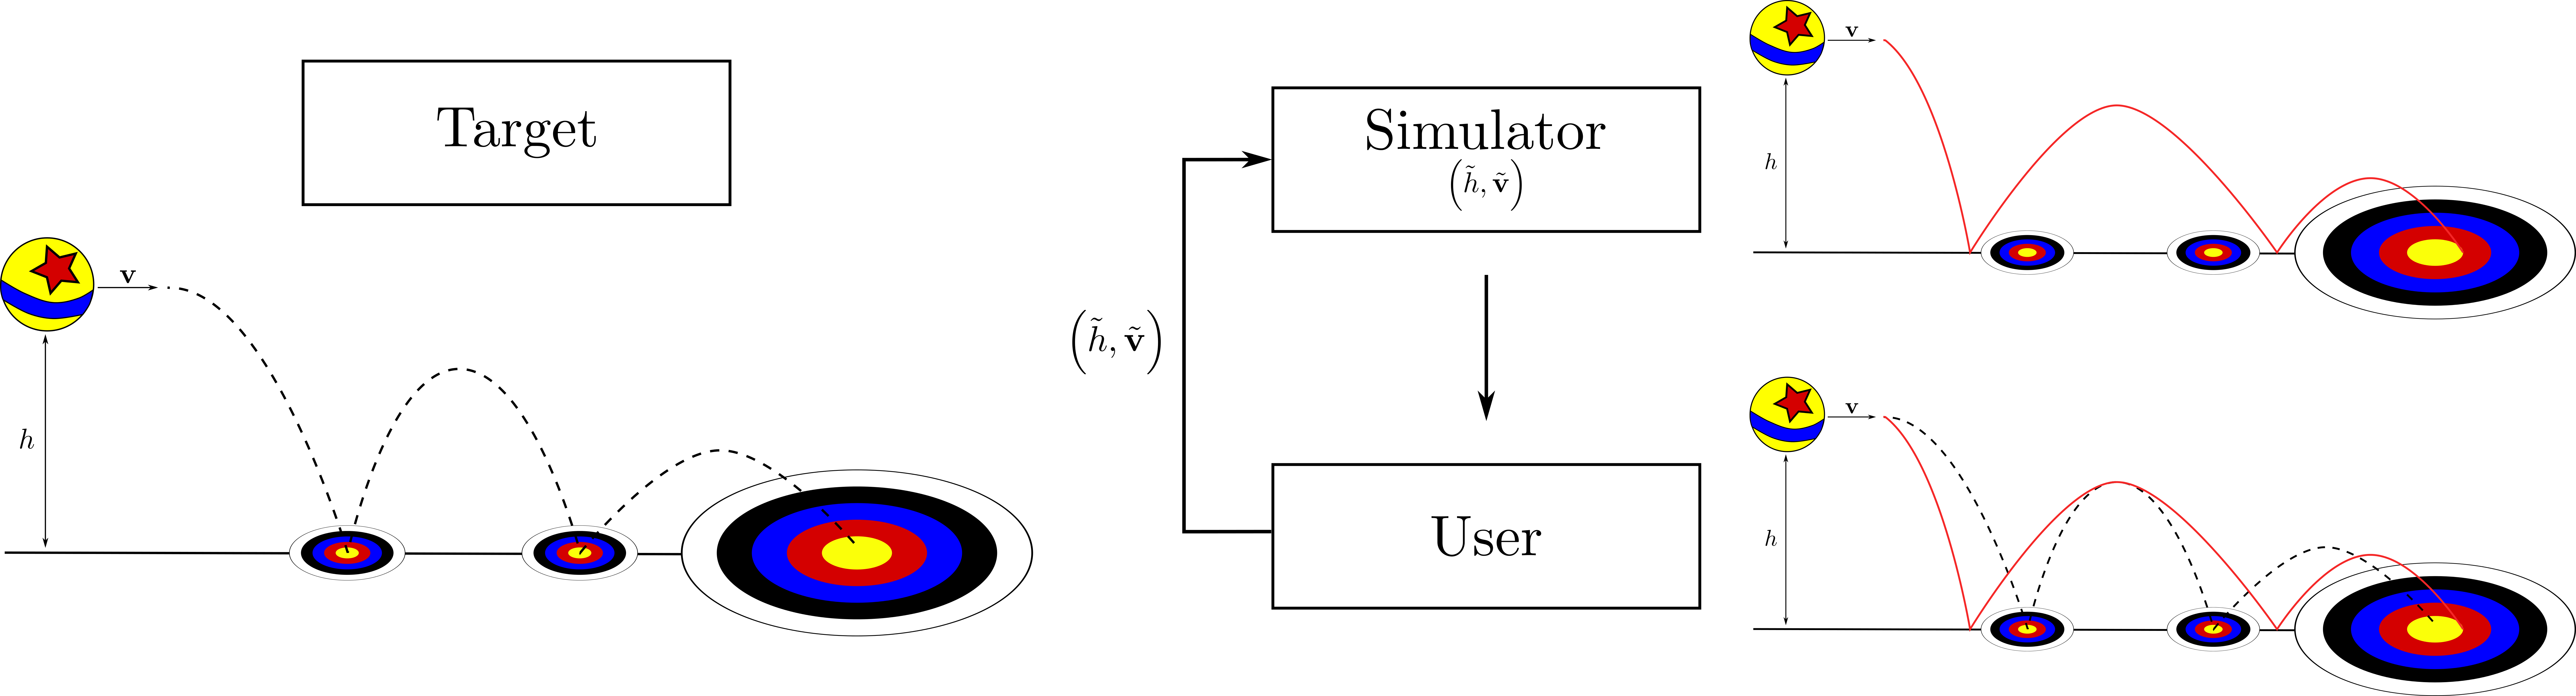
\includegraphics[width=\linewidth]{./images/simulationControl/trialError.png}
	\caption[STAR control: Trial and error process]{\label{fig:trialErrorProcess}Trial and error process. 
	The user runs successive simulations with different parameters such as the initial height $h$ and velocity $\mathbf{v}$ of the ball until it reaches a desired target.}
\end{figure}

There are mainly three constraints which make this task a nightmare:
\begin{itemize}
	\item Firstly, the computational time plays a major role. 
	This is obvious but still important to states. 
	A real-time simulation will allow the user to quickly explore parameters whereas an offline simulation might require days and days of tuning.
    Here, we can mention procedural tools which are generally much more efficient than simulation and therefore enable faster editing loops. Unfortunately they are often limited to overly restrictive models such as large open ocean surfaces~\cite{hinsinger2002,Tessendorf2004,jeschke2015water,horwath2015empirical}.
	\item Secondly, the control is indirect and, most of the time, based on unintuitive parameters which requires some expertise about the underlying physical model. The user cannot directly control the trajectory nor the shape of the object.
	\item Thirdly, many physics-based animations describe a non-linear behavior. Fluid animations are among them for instance. 
	This non-linearity makes it very hard to choose the right parameters. 
	Small changes can produce very different results making tedious to explore the range of possible behaviors and almost impossible to respect specific artistic directions such as timing, key positions, trajectories or shapes. 
	Also, it prevents the user from interactively controlling a low-resolution simulation and then achieve a similar behavior with the same parameters at a higher resolution.
\end{itemize}

\subsection{Space-time constraints paradigm}
A general approach for controlling a physics-based animation is to formulate it as an optimization under constraints: 
"\emph{Find the value of the parameters such that the physical behavior and user constraints are respected over the animation}" 
(see Figure~\ref{fig:spaceTimeConstraints}).
\begin{figure}[!h]
\centering

\includegraphics[width=\linewidth]{./images/simulationControl/spaceTimeConstraints.png}
\caption[STAR control: Space-time constraints]{\label{fig:spaceTimeConstraints} Space-time constraints. 
An optimization problem is defined to find the value of the parameters which solve the equations of motion while respecting constraints defined by the user.
In this example, the parameters are the initial height $h$ and velocity $\mathbf{v}$ of the ball and the constraints are the position of the ball at different time.
The ball has a mass of $1\kilo\gram$ and is only submitted to the gravity $\mathbf{g}$.}
\end{figure}

Four challenges arise, what are the parameters we want to control, what are the user constraints, how to formulate them and finally how to numerically solve the problem. 
Witkin and Kass were among the first to introduce this formulation to the Computer Graphics community in their pioneer work \emph{Space-time constraints}~\cite{Witkin1988}.

\subsubsection{Parameters}
The most common parameters are the positions of the material samples and the external forces.
A common drawback of using external forces is that the necessary changes may become highly unrealistic.
As an alternative, Coros et al.~\cite{Coros2012} proposed to adapt the rest shape of the object from one frame to another in order to induce internal forces that would match the user goals.
When large deformation occurs it is possible that the computed solution is at the limit of the deformation that the object can reach. In order to enforce the optimization, Li et al.~\cite{Li2014} proposed to optimize material parameters as well. 

\subsubsection{Constraints}
Position, velocity and density are among the constraints that are most often used for controlling an animation. 
Of course, they depend on the simulated object: rigid, solids, smoke, liquid, etc. 
Certainly, position constraints are the most intuitive for the user as they can be specified using key-frames. 
However, designing a key-frame for a highly elastic object or viscous materials might be extremely hard to achieve. 
Here there is a direct link to the works about surface modeling which propose to deform naturally an object~\cite{Sorkine2007, Hildebrandt2011}. 
In some cases, these deformation tools can be seen as a local static simulation of the object that computes its deformation from a displacement induced by the user. 
For elastic objects, such deformation tool has been proposed by Barbic et al.~\cite{Barbic2012}.
For liquids, Pan et al.~\cite{Pan2013} propose an interactive method to deform wave shapes by sketching their profiles. 
Thus, direct spatial deformation is made possible. 
Both fits in the framework of surface modeling deformation. 
The only difference is that the functions which are minimized are directly derived from the internal forces acting on the object. 
These methods are particularly useful when interactively editing an animation, specially when they are combined with high level deformation tools such as sketching.

\subsubsection{Numerical solution}
In their work, Witkin and Kass~\cite{Witkin1988} dealt with small systems and short simulation period.
Therefore, they could afford to directly solve the optimization problem, meaning that at each iteration a whole simulation would be computed. For instance, small rigid bodies simulation could be interactively designed through this approach~\cite{Popovic2000,Popovic2003}. For complex models and large simulation time, this approach is intractable. Windowing methods allowed to restrict the optimization to the space-time range of interests~\cite{Cohen1992}. In their work~\cite{McNamara2004} proposed to use the adjoint method to efficiently compute gradients in liquid simulation thus improving the performance of the optimization. The approach was also used by Wojtan et al.~\cite{wojtan2006keyframe} for handling large particle systems. For elastic bodies, the use of reduced model allowed to achieve speed-ups of several order of magnitude, thus allowing to interactively edit a physics-based animation~\cite{Barbic2012,Hildebrandt2012,Hahn2012}. Since, this approach has been further improved to be faster~\cite{Schulz2014} and to deal with large deformations~\cite{Li2014}.

\subsection{Applications \& Alternatives}
The strength of the space-time constraints paradigm relies on its very general definition. Therefore, a large number of applications and methods can be seen as offsprings of this approach. In the following, we distinguish different applications of physics-based animation control and present alternatives to the above methods.

\subsubsection{Enriching an animation with physics}
Given a full animation, a simulation is run in order to enhance the input animation with detailed physically-based secondary motions. This approach was successfully applied to enhance character animation with wrinkles and folds of their skin by Bergou et al.~\cite{Bergou2007}. In their work, they compute the dynamics of thin shells on top of the animation by using a multi-resolution approach. In fluid animation, details enhancing brings a lot of attention as it would be easier to set up low resolution simulation and add details on top of it without loosing the global behavior. A nice approach was proposed by Mercier et al.~\cite{Mercier2015} where they solve a Lagrangian wave simulation only at the surface of the low resolution simulation.

\subsubsection{Guiding a simulation with animation data}
A large number of methods propose to guide a simulation without the need of an expensive optimization problem. 
Generally these methods propose to use external forces that are automatically computed from the user inputs such as key-frames.
One of the first approach of this kind was proposed by Lamouret and Cani~\cite{Lamouret1996}.
This approach was later extended to more involved inputs such as simulation data.
In the case of fluid, user-defined velocity field~\cite{Kim2006:SmokeControl}, distance fields~\cite{Yang2013} and control particles~\cite{Thurey2006:FluidControl,Madill2013} were proposed to control the trajectory of fluid animation.
Still in the same idea, there are many methods which propose to guide the behavior of an object using geometric proxies which are easier to control for an artist than simulation data. For example, artists can use a triangle mesh to specify a target shape which will act as an attractor by adding artificial attraction forces based on the distance to the mesh surface. 
Such approaches have been successfully developed to drive smoke~\cite{Fattal2004,Hong2004,Shi2005a} and liquid simulations~\cite{Shi2005b,Raveendran2012}.
Taking this strategy further, the geometric proxies themselves can be defined by a low-resolution fluid simulation. 
To achieve this, the artist quickly sets up a coarse simulation and uses the output geometry to guide the main features of a full resolution simulation.
Several approaches modify a high-resolution smoke simulation using optimization~\cite{Nielsen2009,Nielsen2010}, patterns extracted as skeleton~\cite{Yuan2011}, or sparse sampling~\cite{Huang2013}.
For liquid simulations, Nielsen and Bridson~\cite{Nielsen2011} propose to restrict the high resolution simulation to a thin layer around a guiding coarse animation.
Although each of these approaches are able to successfully guide an animation, they do not enable direct control of the resulting animation. Designing precise timing or feature scaling would therefore still require iterative trial-and-error steps to converge toward a desired animation.

\subsubsection{Example-based simulation}
Instead of controlling the trajectory of an object, one might want to control how it deforms when it collides with other objects. 
In exampled-based simulations, a set of examples that represent the desired deformations is used to build a space of preferred deformations from where internal forces will be deduced. This method was first introduced by Martin et al.~\cite{Martin2011} for elastic deformations. Jones et al.~\cite{Jones2016} propose a similar method to easily incorporate plastic deformations in rigid bodies simulations.

\subsubsection{Animation sampling}
In multibody systems, the space-time constraints paradigm can hardly be used. In cause, the large number of discontinuous contacts events which makes the optimization problem particularly difficult to solve. In contrast, multibody simulators are particularly fast, so fast that it is possible to run in parallel a large number of simulations. In their work,~\cite{Chenney2000}~and~\cite{Twigg2007} exploit this performance to sample the space of parameters of an animation and thus finding those which satisfy the user constraints.

\subsubsection{Animation editing} 
In contrast with simulation control, animation editing consists in deforming in space and time the output of a simulator without the need to re-simulate.
Closely related to surface modeling it has to take into account the temporal dimension and its relation with space in order to propose new editing tools. 
In these approaches, finding a natural way to deform an animation and ensuring temporal consistency are amongst the main challenges.
Very few methods have been proposed whereas it represents a much faster approach to edit animations.
Among the most interesting approaches, Pighin et al.~\cite{Pighin2004} propose to build a space-time parametrization of a smoke animation using advected radial basis functions. The parametrized data are then deformed using a trajectory-based editing tool.
Schpok et al.~\cite{Schpok2005} proposed to extract and parametrize features such as vortices, uniform advection, sinks and sources to allow the user to modify the parameters in a smoke simulation.
For liquid animations, Raveendran et al.~\cite{Raveendran2014} propose a semi-automatic method to match two liquids animations and smoothly interpolate between them. 
This approach allows to quickly explore parameter space such as boundary conditions or viscosity parameter and then to produce a large number of new liquid animations without the need for re-simulation.

\subsection{Conclusion on simulation control}

All the methods mentioned above make a trade-off between realism and control.
On one hand, realism requires a high computational cost and makes methods such as space-time constraints unattractive for interactive use.
On the other hand, giving the user full control may introduce unphysical and unpleasant behavior.
Very few works explored the edit of an existing animation and how to extend classical modeling techniques to animated content.
We think that this approach would allow to interactively design physics-based animation without the need to re-simulate.
In Chapter~\ref{chap:fluidsculpting}, we will present a system for the design of fluid animation based on this idea.

\section{Conclusion}
There is a large number of techniques and models that are used to improve the efficiency of simulations, to simulate new phenomena and to allow the user to control a simulation.
We begin our contributions by extending an adaptive model, initially proposed for nanosystems simulations, to speed-up particle simulations in Computer Graphics, in Chapter~\ref{chap:arps}.
Then, we study how to perform detailed topological changes with the frame-based model in Chapter~\ref{chap:cutting}, an interesting approach which ensure a very small number of degrees of freedom and therefore interactive performances.
Finally, we explore a new way of editing fluid animations in Chapter~\ref{chap:fluidsculpting}, where the user can manipulate sub-part of the animation interactively without the need to re-simulate.


%\chapter{Adaptively Restrained Particle Simulation: A new approach for adaptive particle simulation}
\label{chap:arps}

\begin{figure}[!h]
    \begin{tabular}{cc}
        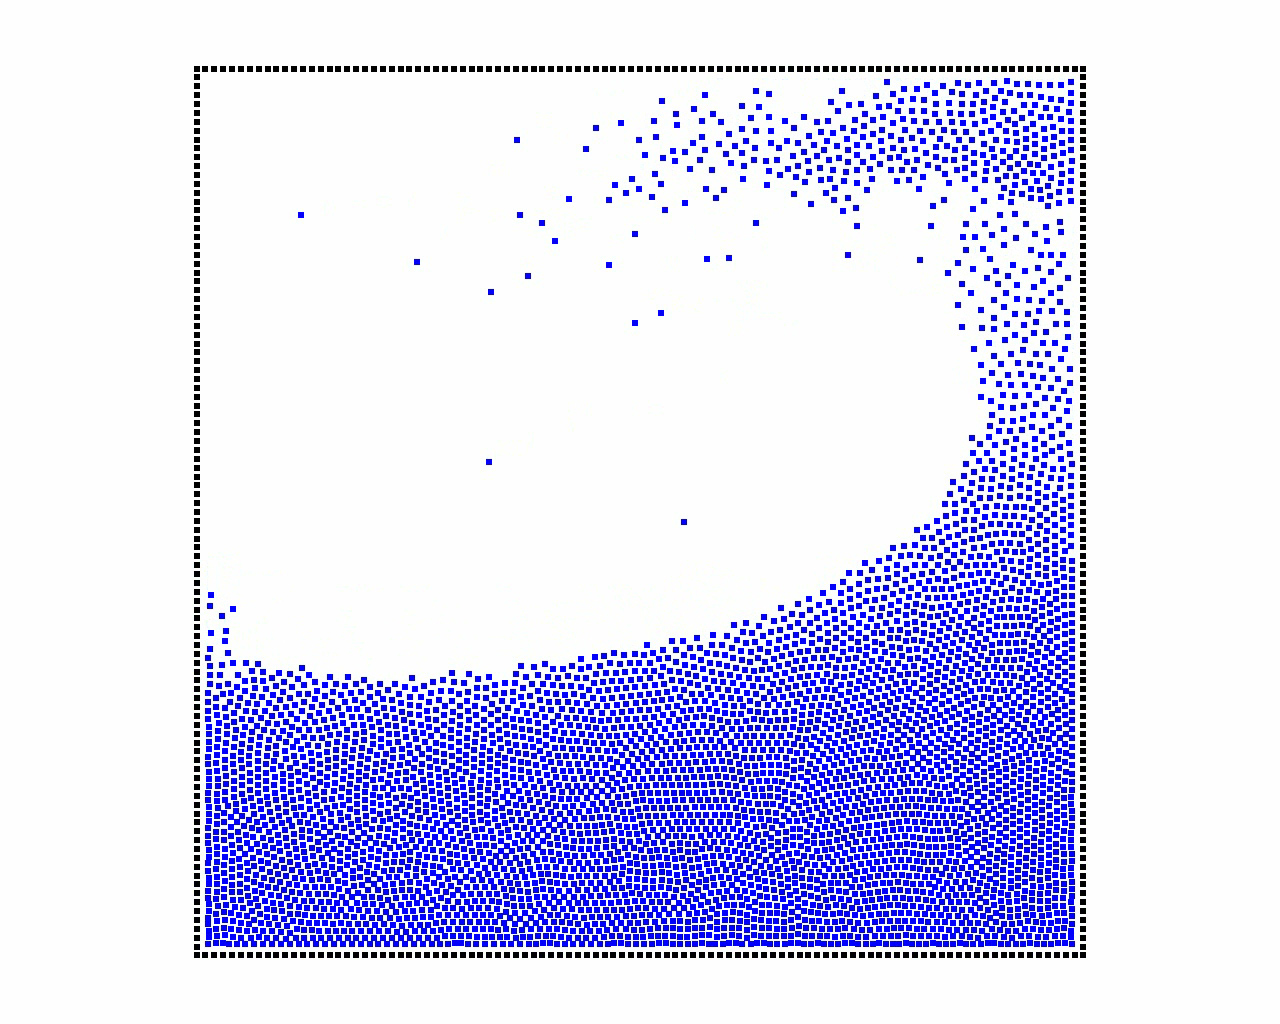
\includegraphics[width=0.4\linewidth]{images/arps-vriphys2013/ReposSPHClassique1.jpg} &
        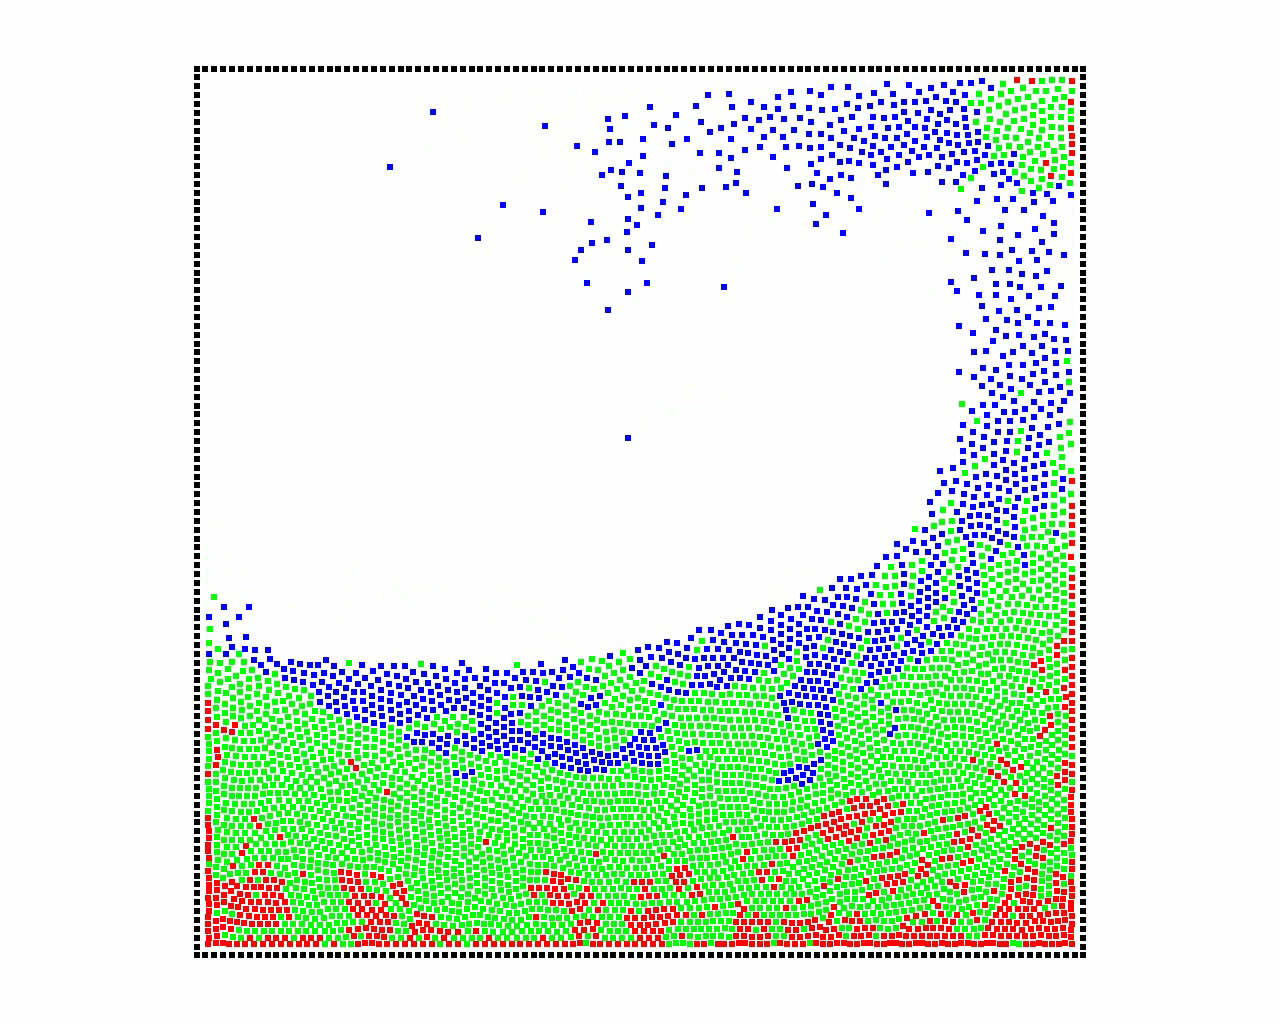
\includegraphics[width=0.4\linewidth]{images/arps-vriphys2013/ReposSPHARPSColor1.jpg}
    \end{tabular}
 \centering
 \caption[ARPS: Dam break simulations]{ A dam break simulation with 5000 particles simulated with WCSPH (on the left)
 and with our adaptive method (on the right). On the right image, blue corresponds to full-dynamics particles, green to transition particles and red to restrained particles.}
\label{fig:teaser}
\end{figure}

Combining efficiency with visual realism had been one of the main goals of Computer Graphics research in the last decade. As presented in section~\ref{sec:starAdaptivity}, the general strategy for efficient graphical simulations is to concentrate the computational time on the most interesting parts of an animated scene (such as near the surface of a fluid), while simplifying the rest of the scene according to some visual quality criteria.  A number of adaptive simulation methods, aimed at controlling the trade-off between performance and precision, have been developed. Most of them consist in changing time or space sampling, using adaptive time steps or multi-scale models.
Although several of them give impressive results, they are often difficult to implement, may-be restricted to specific applications, sometimes generate discontinuity artifacts due to sudden simplifications.
\\ \\
A different approach for adaptive simulation~\cite{Artemova2012} was recently proposed in the context of molecular dynamics~(MD). Contrary to previous methods, Adaptively Restrained Particle Simulations (ARPS) do not adapt time or space sampling, but rather switch the positional degrees of freedom of particles on and off, while letting their momenta evolve. The key idea is that since most of the computation time is spent in computing interaction forces based on positions, particles with low velocity could be considered fixed in space - and the corresponding interaction forces constant - until they accumulate enough momentum to start moving again. Therefore, inter-particles forces do not have to be updated at each time step, in contrast with traditional methods that spend a lot of time there.
\\ \\
While freezing objects to gain computation time has been extensively used in video games, the question of when and how to release them has not been extensively studied, and has mainly relied on \textit{ad hoc} heuristics.
Adaptively Restrained Particle Simulations~(ARPS), in contrast, introduces a physically sound approach with proven correctness, and has been successfully used in the context of predictive, energy- and momentum-conserving particle simulation.
\\ \\
In this chapter, we explore the use of Adaptively Restrained (AR) particles for graphics simulations. We present the initial formulation of ARPS that was introduced for molecular dynamics simulations in Section~\ref{sec:arps_basics}, and explore its potential for Computer Graphics applications. Our contributions are as follows:
\begin{itemize}
\item We adapt ARPS to particle-based fluid simulations and propose an efficient incremental algorithm to update forces and scalar fields in Section~\ref{sec:arps_sph}.
\item We introduce a new implicit integration scheme enabling to use ARPS for stiff objects simulation such as cloth simulation in Section~\ref{sec:arps_implicit}.
\end{itemize}
Practical implementation and parameters tuning are then addressed in Section~\ref{sec:arps_implementation}. We finally discuss results and perspectives in Section~\ref{sec:arps_discussion}. Our experiments show that this new, simple strategy for adaptive simulations can provide significant speedups more easily than traditional adaptive models.

%-------------------------------------------------------------------------
\section{Adaptively Restrained Particles} 
\label{sec:arps_basics}
%-------------------------------------------------------------------------
\paragraph*{Basic ideas:}
Adaptively Restrained Particle Simulations (ARPS)~\cite{Artemova2012} was recently developed to speed up particle simulations in the field of Molecular Dynamics.
They rely on Hamiltonian mechanics, where the state of a system is described by a position vector $\vec q$ and a momentum vector $\vec p$, and its time evolution is governed by the following differential equations:
\begin{eqnarray*}
\frac{d\vp}{dt} &=& -\frac{\partial \H}{\partial \vq} \\
\frac{d\vq}{dt} &=& +\frac{\partial \H}{\partial \vp}
\end{eqnarray*}
Here, the Hamiltonian $\H$ is the total mechanical energy given by:
\begin{equation}
    \label{eq:hamiltonian}
    \H(\vq,\vp) = \frac{1}{2} \vp^{T}M^{-1}\vp + V(\vq)
\end{equation}
where the first term corresponds to the kinetic energy, while the second represents the potential energy.
In \cite{Artemova2012}, an \textit{adaptively restrained} (AR) Hamiltonian is introduced:
\begin{equation}
    \label{eq:arhamiltonian}
    \H_{AR}(\vq, \vp) = \frac{1}{2} \vp^{T}\Phi(\vq,\vp)\vp + V(\vq)
\end{equation}
The matrix $\Phi$ is a block-diagonal matrix used to switch on or off the positional degrees of freedom of the particles during the simulation.
Each $3$x$3$ block corresponds to a particle $i$ equal to
$\Phi_{i}(q_{i}, p_{i}) = m_{i}^{-1}[1 - \rho_{i}(q_{i}, p_{i})]\mathbf{I_{3\mathtt{x}3}}$.
The function $\rho_{i} \in [0, 1]$ is called the \emph{restraining function}.
When $\rho_{i} = 0$, $\Phi_{i} = m_{i}^{-1}$ and the particle is \textit{active}: it obeys standard (full) dynamics.
When $\rho_{i} = 1$, $\Phi_{i} = 0$ and the particle is \textit{inactive} (not moving). When $\rho_{i} \in [0, 1]$, the particle is in transition between the two states.
%-------------------------------------------------------------------------
The restraining function $\rho_{i}$ of each particle is used to decide \emph{when} to switch positional degrees of freedom on or off.
In \cite{Artemova2012}, $\rho_{i}$ depends on the particle kinetic energy.
The function uses two thresholds, a restrained-dynamics threshold $\epsilon^{r}$ and a full-dynamics threshold $\epsilon^{f}$.
It is defined as :
\begin{equation}
    \label{eq:restrainingfunction}
    \rho_{i}(p_{i}) =
    \displaystyle\left\lbrace
    \begin{array}{lccc}
        1, & & & \textrm{if } 0 \leq K_{i}(p_{i}) \leq \epsilon_{i}^{r} \\
        0, & & & \textrm{if } K_{i}(p_{i}) \geq \epsilon_{i}^{f} \\
        s(K_{i}(p_{i})) \in [0, 1], & & & \textrm{elsewhere} \\
    \end{array}
    \right.
\end{equation}
where $K_i=p_i^2/2m_i$ is the kinetic energy, and
$s$ is a twice-differentiable function. In practice a $5^{th}$-order spline is used.
%-------------------------------------------------------------------------
\paragraph*{Adaptive equations of motion:}
The adaptive equations of motions are derived from the AR Hamiltonian (\ref{eq:arhamiltonian}):
$$
%     \label{eq::armotionequation}
    \begin{array}{l}
        \displaystyle \frac{d\vp}{dt} =
        -\frac{\partial \H_{AR}}{\partial \vq} = -\frac{\partial V(\vq)}{\partial \vq} \\
        \displaystyle \frac{d\vq}{dt} =
       \frac{\partial \H_{AR}}{\partial \vp} = M^{-1}[I - \rho(\vp)] \vp
        - \frac{1}{2}\vp^{T}M^{-1}\frac{\partial \rho(\vp)}{\partial \vp}\vp\\
    \end{array}
$$
Applied to a particle, one can derive the rate of position change, which we call \textit{effective velocity}, as:
\begin{equation}
    \label{eq:adaptiveVelocity}
    \dot{q} = \frac{1}{m}\left((1-\rho(p))p - \frac{1}{2}\parallel p \parallel^2\frac{\partial \rho(p)}{\partial p}\right)
\end{equation}
While the momenta evolve as in classical Hamiltonian mechanics, position evolves differently.
When a particle's momentum is small enough, the particle becomes inactive and stops moving.
However, even if the particle is inactive, its momentum may change.
Therefore its kinetic energy may become large enough again for the particle to resume moving.
In general, particles switch between active and inactive states during the simulation.
%-------------------------------------------------------------------------
\begin{figure}[htb]
  \centering
  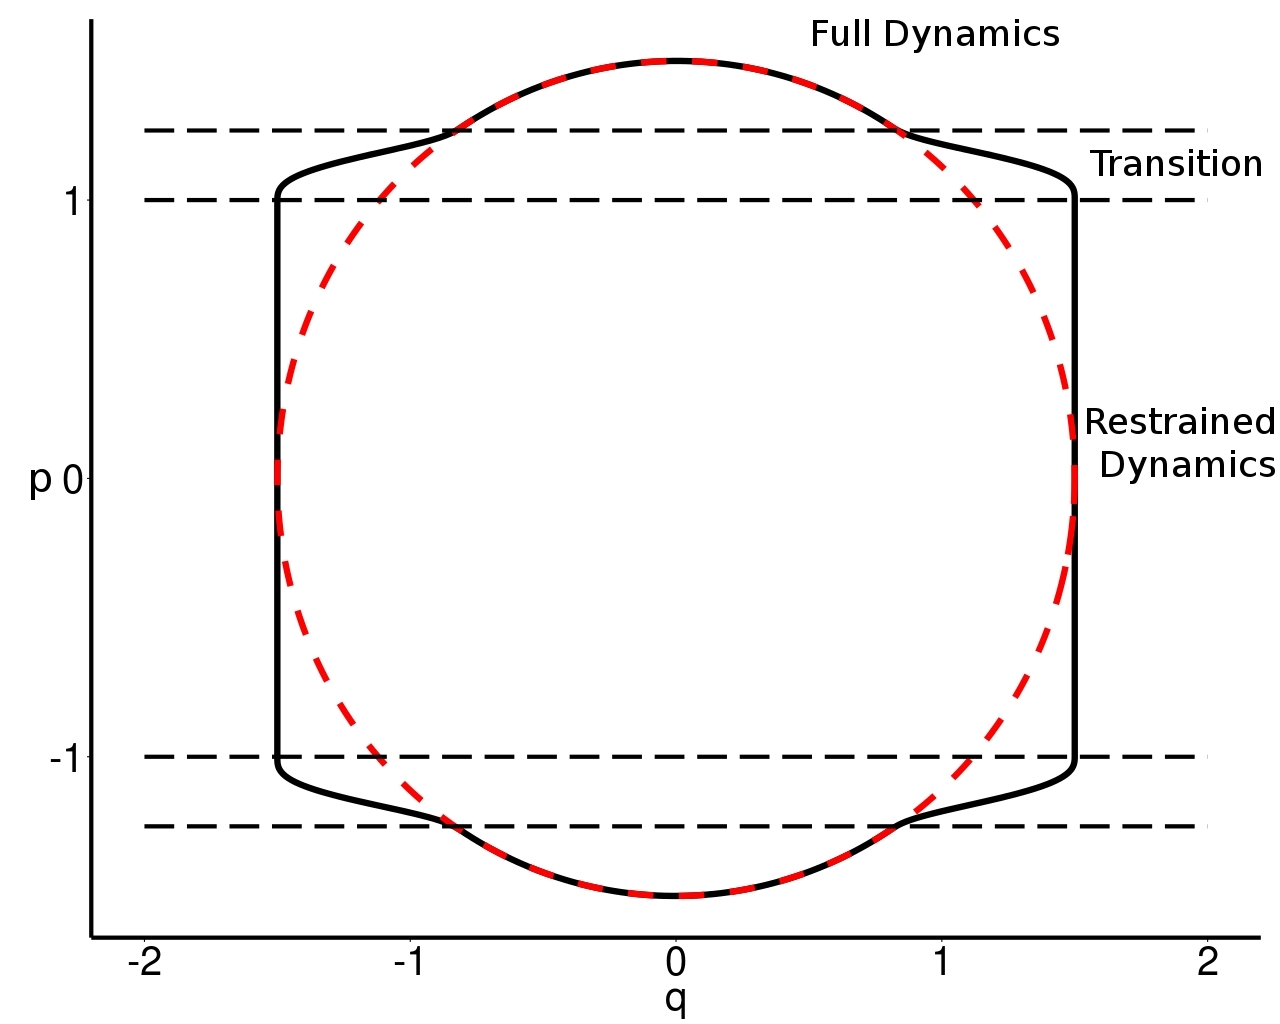
\includegraphics[width=0.8\linewidth]{images/arps-vriphys2013/harmonicOscillatorPhasePortraitraw.jpeg}
  \caption[ARPS: Phase portrait of a ARPS harmonic oscillator]{\label{fig:harmonicOscillatorPhasePortrait} Phase portrait of a harmonic oscillator. The red dotted ellipse corresponds to standard Hamiltonian mechanics, while the solid black line corresponds to ARPS. During restrained dynamics momentum is accumulated. Then a transition deals with the accumulated energy before getting back to the full dynamics.}
\end{figure}

\paragraph*{A simple example:}
Consider a 1D harmonic oscillator : a particle attached to the origin with a perfect spring.
Fig. \ref{fig:harmonicOscillatorPhasePortrait} shows a phase portrait of the corresponding
AR system.
In classical mechanics, the trajectory of the state in this (position, momentum) space is an ellipse, the size of which depends on the (constant) energy of the system.
Using ARPS, the position is constant (vertical straight parts) as long as the kinetic energy is small enough, while it is an ellipse as long as the kinetic energy is big enough.
These trajectories are connected by a transition corresponding to an energy between the two thersholds of eq.~(\ref{eq:restrainingfunction}).
The closed trajectory corresponds to a constant \textit{adaptively restrained energy} $H_{AR}$.

\paragraph*{Generalization:}
Due to the similarity of the adaptive kinetic energy with the standard kinetic energy, one can show that particle systems simulated using ARPS exhibit the expected properties of standard physical simulation, namely the conservation of momentum and (adaptive) energy.
It is therefore possible to perform macroscopically realistic simulations with reduced computation time.

%-------------------------------------------------------------------------
\paragraph*{Computational performance:}
\cite{Artemova2012} obtained significant speedup exploiting immobility of particles.
An incremental method was used to update the particles forces at each time step, while saving time on inactive particles :
\begin{enumerate}
    \item All forces that were acting on each active particle at the previous time step are substracted based on previous position.
    \item New forces based on current positions are added to each active particle.
\end{enumerate}
The computational performance comes from the absence of force computation between
two inactive particles and the absence of neighbor search for inactive particles.
As these two steps are common bottlenecks in particle simulation, significant speedup were achieved.

%-------------------------------------------------------------------------
\paragraph*{Potential benefits of extension to Computer Graphics:}
Molecular dynamics often inspired particle-based simulations in Computer Graphics. The same bottleneck, namely inter-particles forces computation based on neighbor search, is present in the two fields, so we can expect interesting performance for ARPS in graphics. The remainder of this chapter explores two applications of ARPS to graphical simulations:
\begin{enumerate}
\item Particle-based fluid simulation. In this case, damping forces are involved in contrast with the classic use of ARPS.
We propose a method to handle them as well as an incremental algorithm to update the forces and the scalar fields.
\item Stiff object simulation. We take the example of a cloth simulation.
We will propose an implicit formulation of ARPS and a hybrid solver to exploit inactivity of particles.
\end{enumerate}
It is clear that ARPS is not well-suited for simulations where all degree of freedom move: classical spatial adaptation is better suited in this case. In contrast, ARPS is best suited for simulations where most parts are immobile but may resume moving at any time. Even if these situations are not the most visually exciting, they are very common in Computer Graphics: they include simulation of characters clothing when many of the characters are at rest, surgical simulations with local user interaction, and the animation of large volumes of liquid, when most of it already came to rest.

%-------------------------------------------------------------------------
\section{ Extension to SPH fluid simulation } 
\label{sec:arps_sph}
As presented in section~\ref{subsubsec:starSPH}, SPH fluid simulation is widely used in computer graphics and many methods have been proposed \cite{Desbrun:1996:SPN}, \cite{Muller2003}, \cite{Solenthaler2009}, \cite{implicitSPH}.
SPH approximates fluid dynamics with a set of particles.
The particles are used to interpolate properties of the fluid anywhere in the space.
Each particle samples fluid properties such as density, pressure or temperature. All these properties are updated based on the particle neighbors and are
used in short-ranged inter-particle forces.
For a detailed and comprehensive introduction to SPH, you can refer to \cite{Monaghan2005}.
To integrate ARPS, we chose WCSPH (Weakly Compressible Smoothed Particle Simulation) \cite{Becker2007WCSPH}, a standard SPH formulation \cite{Desbrun:1996:SPN}, \cite{Muller2003}.
We limited our simulation to the main inter-particles forces: pressure and viscosity.
Classically a SPH algorithm follows three steps:
\begin{enumerate}
	\item Update mass density and pressure
	\item Compute inter-particles forces : pressure, viscosity
	\item Integrate velocities and positions
\end{enumerate}
With ARPS, time can be saved on each computation step involving pairwise terms.
In SPH, inter-particles forces and density field computation are the perfect candidates.
As proposed in \cite{Artemova2012}, we use an incremental algorithm to update only quantities involving active particles.
%-------------------------------------------------------------------------------
\subsection{Viscosity}
Viscosity forces involve particles velocities. The viscosity force of particle $i$ with respect to particle $j$ is :
\begin{equation}
	\label{eq:viscosityForces}
	f_{ij} =
	\left\lbrace	
	\begin{array}{lrr}
	-m_{i}m_{j}\Pi_{ij}\nabla W_{ij} & & v_{ij}^{T}q_{ij}<0\\
	& & \\
	0 & & v_{ij}^{T}q_{ij} \geq 0 \\
	\end{array}		
	\right.
\end{equation}
$\Pi_{ij}$ is given as :
\begin{equation}
\label{eq:pij}
	\Pi_{ij} = -\nu\left( \frac{v_{ij}^{T}q_{ij}}{ \mid q_{ij} \mid^{2} + \epsilon h^{2} } \right)
\end{equation}
$W_{ij}$ denotes a convolution kernel, $v_{ij}$ the difference of velocities between the two particles, $q_{ij}$ the difference of positions between the two particles, $m_{i}$ is the mass, $h$ is the particle smoothing radius and $\nu = \frac{2 \alpha h c_{s}}{ d_{i} + d_{j} }$ is a viscous term where $\alpha$ is a viscosity constant,
$d_{i}$ the particle $i$ density.
$\epsilon=0.01$ is a constant to avoid singularities.
\newline \newline
However, velocity is not explictly represented in ARPS, and can be seen in two different ways. We may define it based on the momentum and set $ v_{i} = p_{i} / m_{i} $, or based on the change of position $  \dot{q}_{i}$.
In the first case, we can get time-varying forces even for inactive particles, which we want to avoid.
We therefore use the effective velocity of the particle, as defined in eq.(\ref{eq:adaptiveVelocity}).
Applied to a harmonic oscillator, this results in the behavior illustrated in Fig. \ref{fig:HODampedPP}.
The more the particle is damped the longer it remains inactive, which is an intuitive behavior.
%%% HARMONIC OSCILLATOR DAMPED%%%
\begin{figure}[htb]
  \centering
  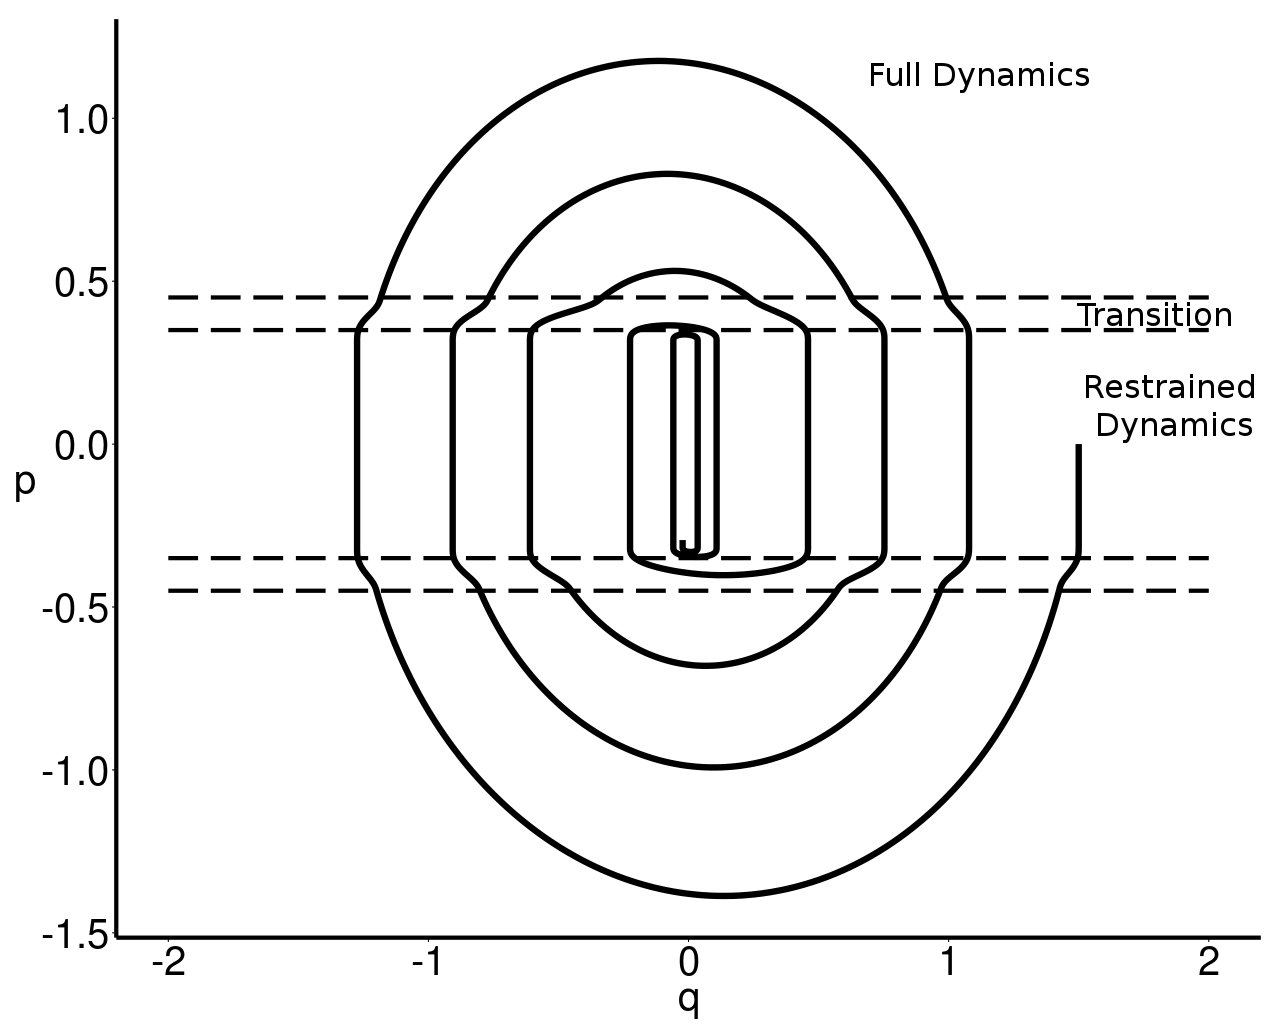
\includegraphics[width=0.8\linewidth]{images/arps-vriphys2013/harmonicOscillatorDampedPhasePortraitraw.jpeg}
  \caption[ARPS: Phase portrait of a damped ARPS harmonic oscillator]{\label{fig:HODampedPP} Phase portrait of our damping approach in ARPS.
  As with a classic damped oscillator we obtain a spiral phase portrait.}
\end{figure}
%-------------------------------------------------------------------------
\subsection{Modified inactivity criterion}
Since our damping force vanishes along with the effective velocity of the particle, it drags down the kinetic energy asymptotically close to the inactivity threshold, without ever reaching it.
Consequently, particles only subject to damping forces never become inactive, and we do not spare computation time, even when the particles get nearly static.
To remedy this problem, we consider inactive the particles which effective velocity fall below a user-defined threshold.
%-------------------------------------------------------------------------
\subsection{Performance}
We performed two experiments to measure computation time.
The first one (Table~\ref{table:perf1}) is a fall of $5000$ particles in a box.
As soon as most particles come to rest, and become inactive the speedup can be significant.
For $15$s, the mean speedup is $3.8$.
The speedup can locally reach $25.7$.
\begin{table}[htb]
   \centering
\begin{tabular}{|c|c|c|c|} \hline
    Simulation Time & SPH   & ARPS    & Speed-up \\ \hline
    15s     & 893s   & 232s                 &  \{0.91, 25.73, 3.85\}\\ \hline
\end{tabular}
\caption[ARPS: Fall of a block of water - Measurements]{\label{table:perf1}Fall of a block of water - Computation time and speedup \{min, max, mean\}}
\end{table}
We can see in Figure~\ref{fig:teaser} that during speed movements most of the particles are active so that the adaptive simulation stay close to reference simulation.
Therefore small scale details like splashes can be preserved.
\begin{figure*}[!ht]
    \centering
    \begin{tabular}{ccc}
        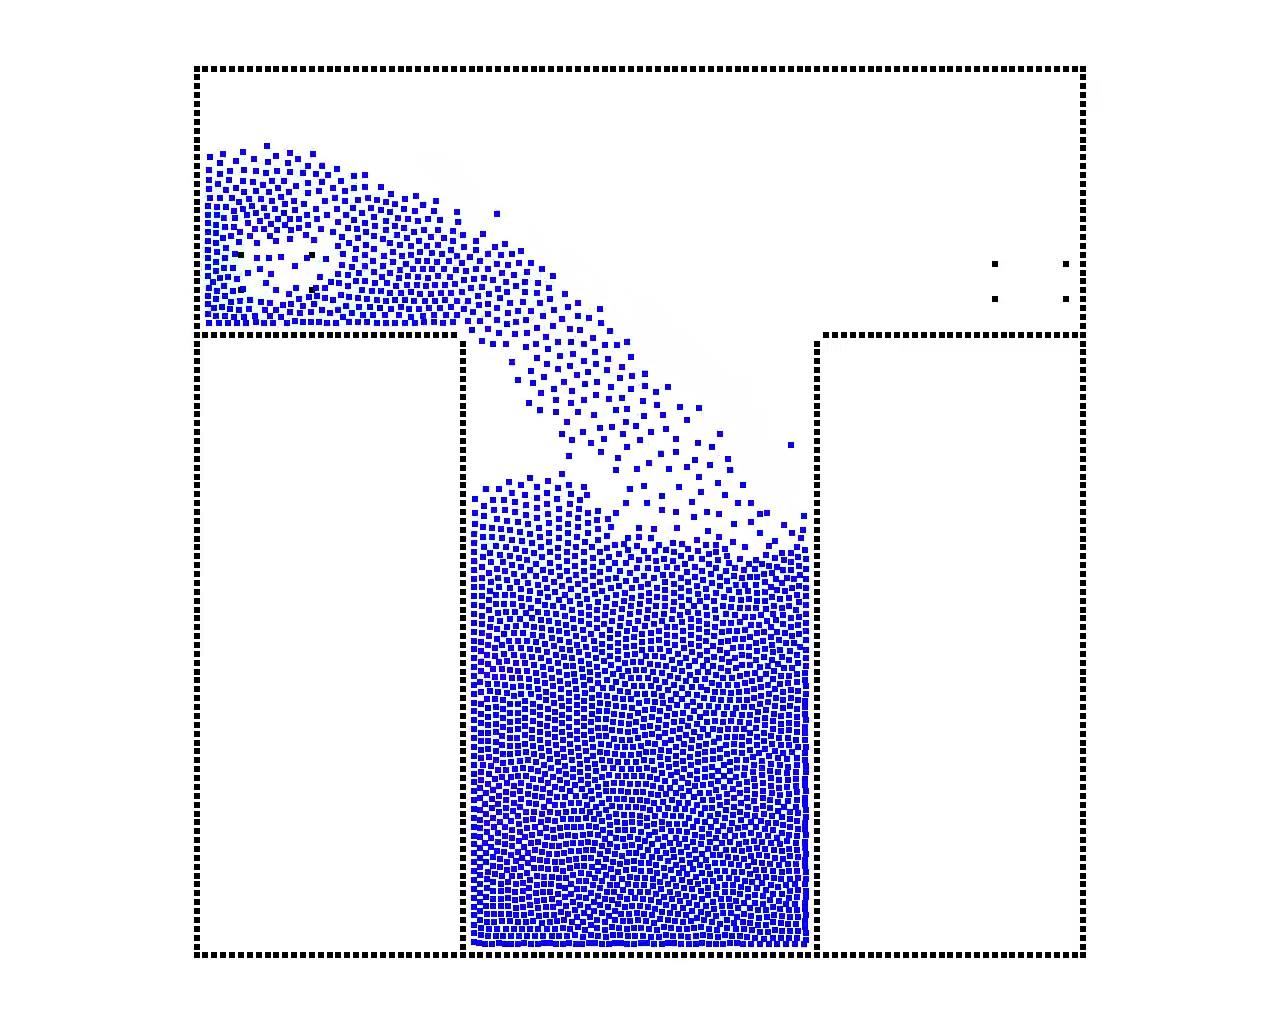
\includegraphics[width=.32\linewidth]{images/arps-vriphys2013/PermanentFlowSPH.jpg} &
        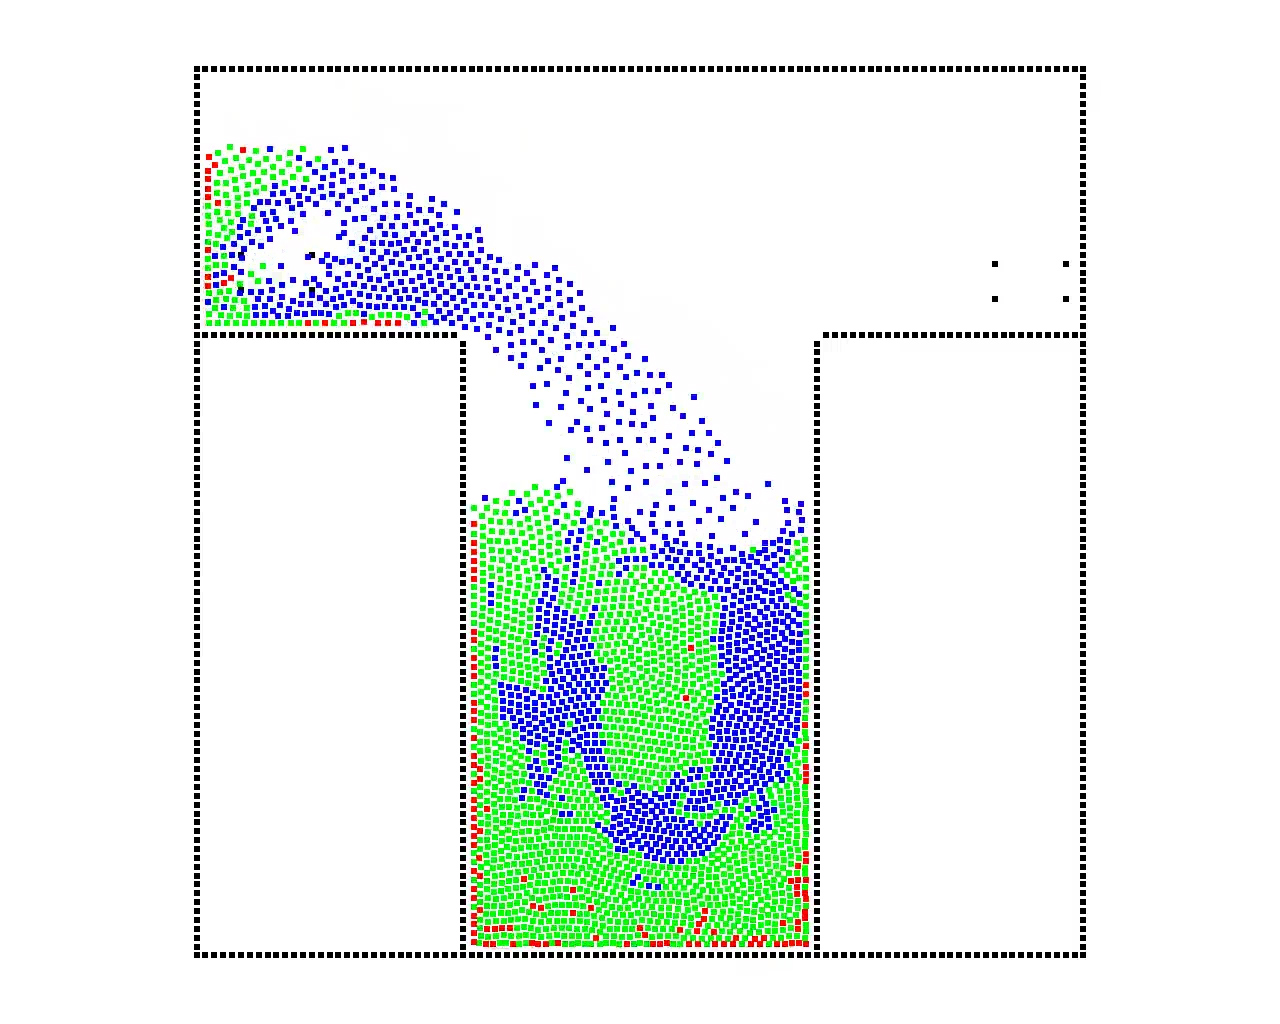
\includegraphics[width=.32\linewidth]{images/arps-vriphys2013/PermanentFlowARPSColor.jpg} &
  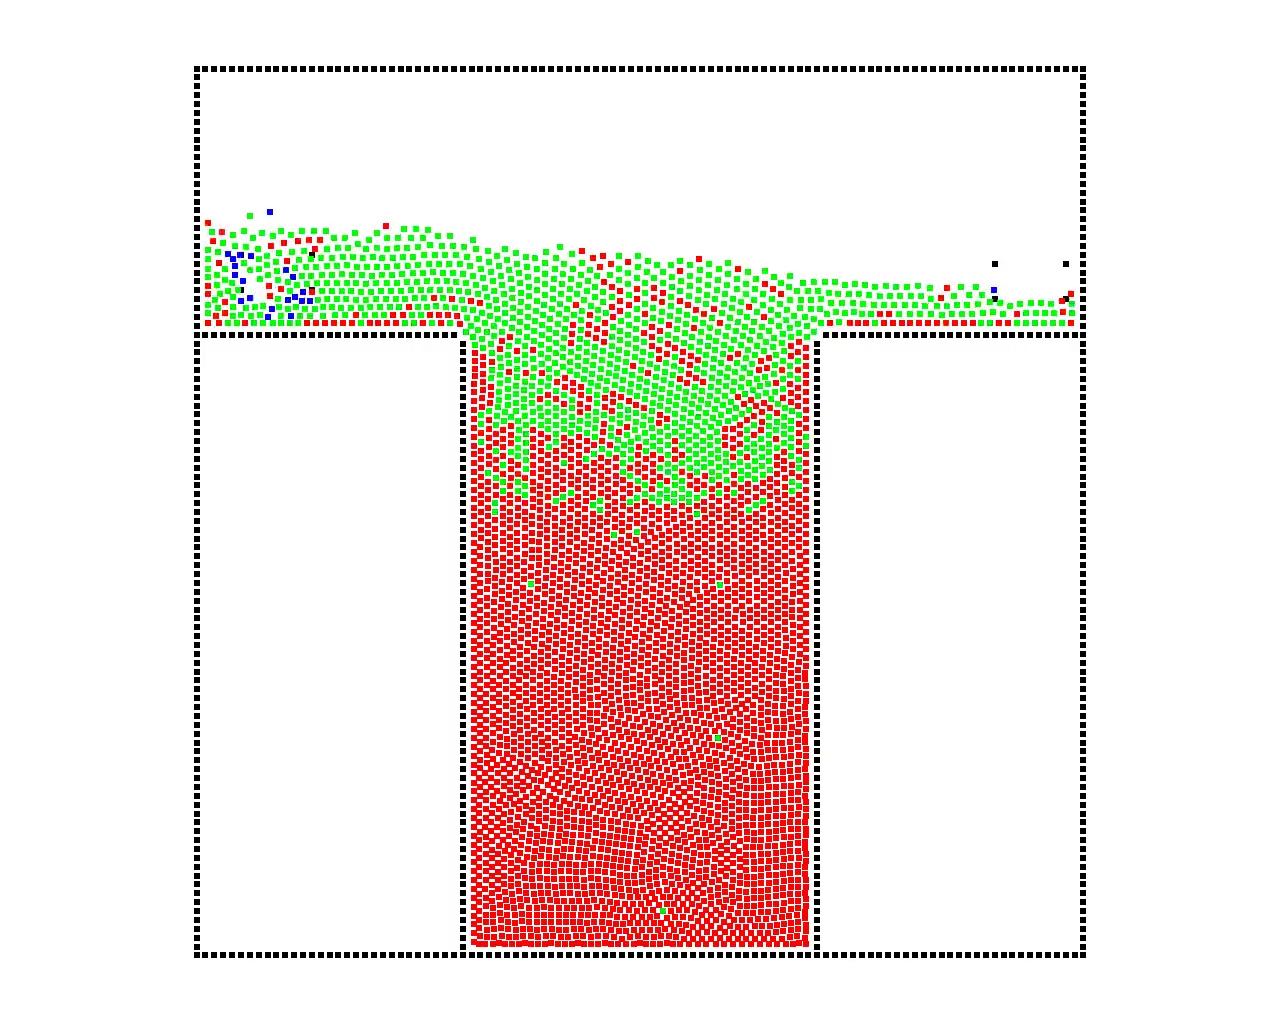
\includegraphics[width=.32\linewidth]{images/arps-vriphys2013/PermanentFlowARPSColor2.jpg} \\
  (a) & (b) & (c)
    \end{tabular}
    \caption[ARPS: Permanent flow simulations]{\label{fig:permanentflow} A permanent flow simulation with 4240 particles.
    (a) is a classic WCSPH simulation. (b) is our adaptive method at the same time of (a) with restrained particles in red. (c) is our adaptive method once the permanent flow is installed.}
\end{figure*}
\newline
The second experiment (see Table~\ref{table:perf2}) is the creation of a permanent flow with $4240$ particles. As we can see in Figure~\ref{fig:permanentflow}, once the permanent flow is installed a large amount of particles are restrained. We reach an interesting speedup while keeping a motion close to the reference.
\begin{table}[htb]
    \centering
\begin{tabular}{|c|c|c|c|} \hline
    Simulation Time & SPH       & ARPS    & Speed-up \\ \hline
    30s         & 2166s     & 814s              & \{0.83, 3.99, 2.66\} \\ \hline
\end{tabular}
\caption[ARPS: Fluid permanent flow - Measurements]{\label{table:perf2}Fluid permanent flow - Computation time and speedup \{min, max, mean\}.}
\end{table}
%-------------------------------------------------------------------------
\section{Extension to stiff objects: Implicit Integration} 
\label{sec:arps_implicit}
In this section we explore the application of ARPS to stiff object simulation and propose an implicit integration scheme which saves computation time for particles at rest.
Implicit integration for cloth simulation was introduced in \cite{Baraff1998}. An introduction to implicit integration is proposed in \cite{Witkin2001}.
While originally formulated on velocity, it can be straightforwardly expressed on momentum.
Instead of integrating the momentum using the forces at the current time step, implicit integration uses the forces at the end of the current step.
As we do not know these forces we end up with a non linear function and after linearization with a linear system to solve to obtain the next momentum:
\begin{equation}
    \label{eq:implicit}
    ( I -h^{2}KM^{-1} ) \Delta p = h( f + h KM^{-1}p ) \;,
\end{equation}
where $\displaystyle K = \frac{\partial f}{ \partial q}$ is the stiffness matrix and
$M$ is the mass matrix.
Solving the linear system is more costly than explicit integration, but it allows the use of larger time steps without any loss of stability, enabling to advance much faster.
%------------------------------------------------------------------------
\subsection{ ARPS Implicit Integration }
We derive an implicit integration scheme from Adaptively Restrained equations of motion.
The linear system has to take into account the state of the particles.
The discrete equations of motions for implicit Euler are:
\begin{equation}
	\label{eq:implicitEqMotion}
	\begin{array}{l}
	\displaystyle \Delta p =  h f(q_{n+1}, p_{n+1})\\
				\\
	\displaystyle \Delta q = h \left( M^{-1}(1-\rho(p_{n+1}))p_{n+1} \right. \\
	\displaystyle \left. - \frac{1}{2	}p_{n+1}^{T} M^{-1} \frac{\partial \rho(p_{n+1})}{\partial p}p_{n+1} \right)
	\end{array}
\end{equation}
We perform a Taylor-Young expansion of $f(q_{n+1}, p_{n+1})$ and introduce $\Delta q$ in the expended momenta equation.
We then perform a Taylor-Young expansion of $\rho(p_{n+1})$ in the momentum equation, which gives us the following equation system:
\begin{equation}
	\label{eq:arpsLinearSystem}
	( I -h^{2}KRM^{-1} ) \Delta p = h( f + h KM^{-1}s )
\end{equation}
$R$ is a block-diagonal matrix where each $3\times 3$ block $R_{ii}$ is:
\begin{equation}
	\label{eq:Ri}
	\begin{array}{l}
	\displaystyle R_{ii} = I - \rho(p^{i}_{n}) - p^{i}_{n} \frac{\partial \rho(p^{i}_{n})}{\partial p_{i}}^{T} \\
	\displaystyle - \frac{1}{2}p^{i}_{n}p^{i^{T}}_{n}\frac{\partial^{2} \rho(p^{i}_{n})}{\partial p_{i}^{2}}^{T} -
	\displaystyle \frac{\partial \rho(p^{i}_{n})}{\partial p_{i}} p^{i^{T}}_{n} \;,
	\end{array}
\end{equation}
while $s$ is a $3N$ vector where $N$ is the number of particles, and each $s_{i}$ is :
\begin{equation}
	\label{eq:si}
	\displaystyle s_{i} = p^{i}_{n} - \rho(p^{i}_{n})p^{i}_{n} - \frac{1}{2	}p^{i^{T}}_{n}p^{i}_{n}\frac{\partial \rho(p^{i}_{n})}{\partial p_{i}}
\end{equation}
Note that if all particles are inactive then we have $R = 0$ and $s = 0$ and we get an explicit formulation:
\begin{equation}
    \label{eq:ARPSImplicitRestrained}
    I \Delta p = h f
\end{equation}
Conversely, if all particles are active then $R = I$ and $s = p$ and we get the classical implicit formulation of eq.(\ref{eq:implicit}).
We loop over time using algorithm \ref{alg:ARPSimplicit}.
\begin{algorithm}[H]
    \caption[ARPS: Implicit integration scheme]{Implicit integration scheme}
    \label{alg:ARPSimplicit}
    \begin{algorithmic}[10]
	\For{ each time step}
	    \State compute $\rho, R, s, f$.
	    \State compute $A = I - h^{2}KRM^{-1}$
	    \State compute $b = h f + h^{2}KM^{-1}s$
	    \State solve $A \Delta p = b$
            \State compute $p_{n+1} = p_{n} + \Delta p$
	    \State compute $\displaystyle q_{n+1} = q_{n} +
            hM^{-1}\left( R\Delta p+ s \right)$
	\EndFor
    \end{algorithmic}
\end{algorithm}
\begin{figure}[htb]
  \centering
  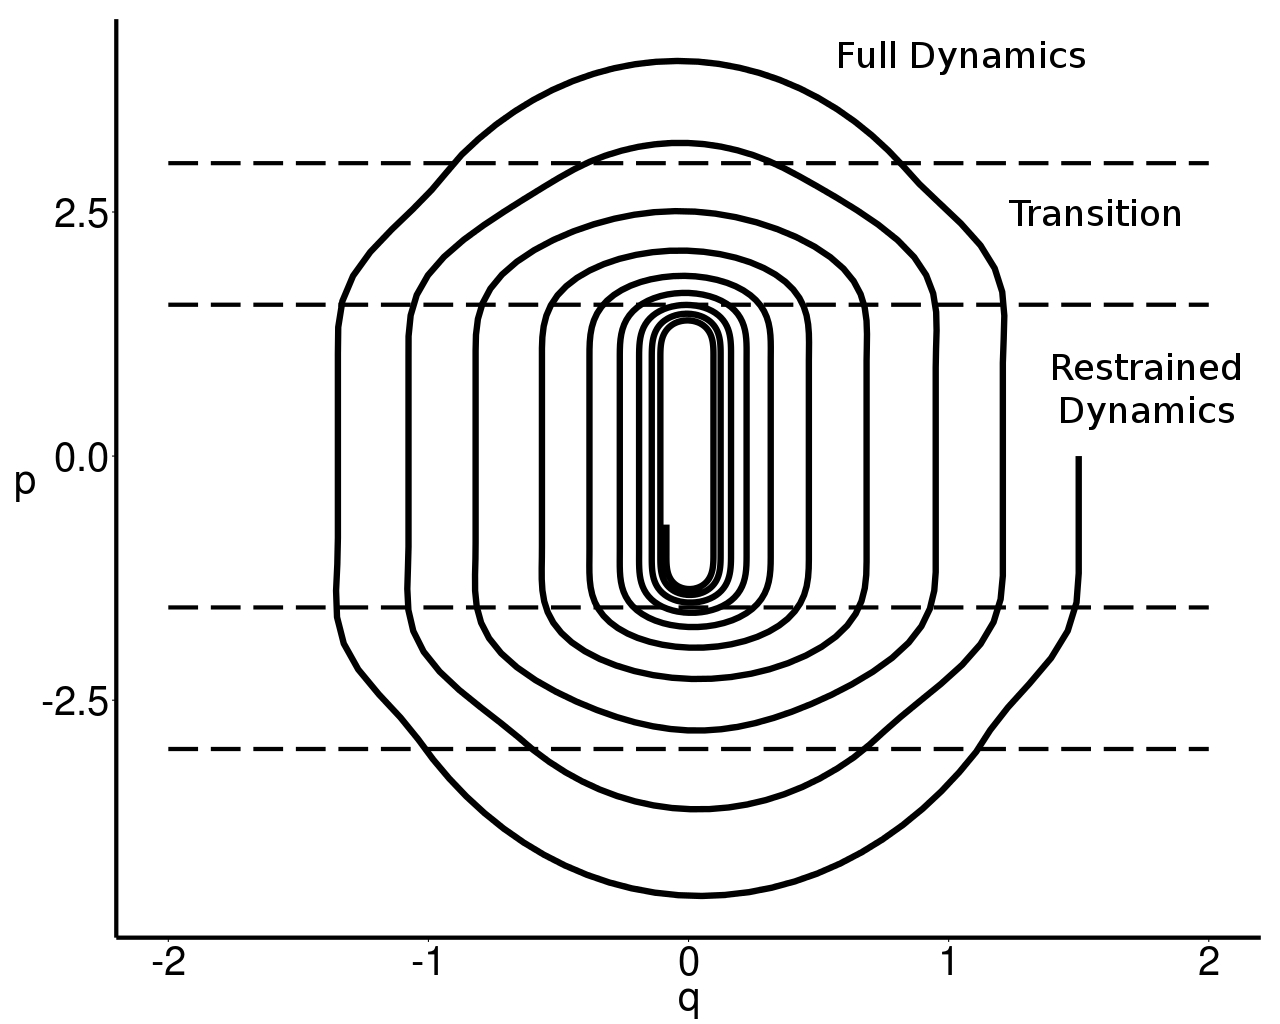
\includegraphics[width=0.8\linewidth]{images/arps-vriphys2013/implicitHOPPraw.jpeg}
  \caption[ARPS: Phase portrait of an implicit ARPS harmonic oscillator]{\label{fig:implicitHOPP} Phase portrait of a harmonic oscillator simulated using implicit ARPS.}
\end{figure}

Figure~\ref{fig:implicitHOPP} shows the phase portrait of a harmonic oscillator simulated using our implicit formulation.
As expected, the well-known numerical damping effect of implicit Euler provides us with the same behavior we could observe with a damped harmonic oscillator.
%%% IMPLICIT HARMONIC OSCILLATOR DAMPED%%%
To include a damping term in the physical model, we derived an implicit formulation which includes a damping term $f_{d} = -\gamma \dot{q}$:
\begin{equation}
	\label{eq:arpsLinearSystemDamped}
	( I + h\gamma M^{-1}R -h^{2}KRM^{-1} ) \Delta p = h( f + h KM^{-1}s + f_{d})
\end{equation}
%------------------------------------------------------------------------
\paragraph*{Solving the equation:}
We exploit inactive particles to save computation time.
As discussed earlier, inactive particles can be handled using explicit integration, which is much simpler.
When a particle is inactive and has no active neighbors we do not need to include it in the linear system.
We thus build the minimal linear system, which only contains active particles and their neighbors.
These particles are implicitly integrated, while the others are explicitly integrated.
\begin{table}[htb]
    \centering
\begin{tabular}{|c|c|c|c|} \hline
    Simulation & Implicit  & Hybrid    & Speed-up \\
    Time & & & \\ \hline
    20s             & 16.9s     & 6.2s      &  \{0.77, 15.16, 2.73\}\\ \hline
\end{tabular}
\caption[ARPS: Implicit vs. Hybrid solver - Measurements]{\label{tab:clothePerf}Implicit solver vs Hybrid solver. Computation time and speedup \{min, max, mean\}.}
\end{table}
Figure~\ref{fig:clothARPS} shows a hanging cloth with active and inactive particles.
At the beginning all the particles become active. Then a moving front of inactivation/reactivation traverses the cloth at decreasing frequency. The cloth finally finds a rest position, where all the particles are inactive and simulated explicitly, saving computation time. The particles can become active again if external forces or imposed motion are applied.
\begin{figure}[htb]
  \centering
  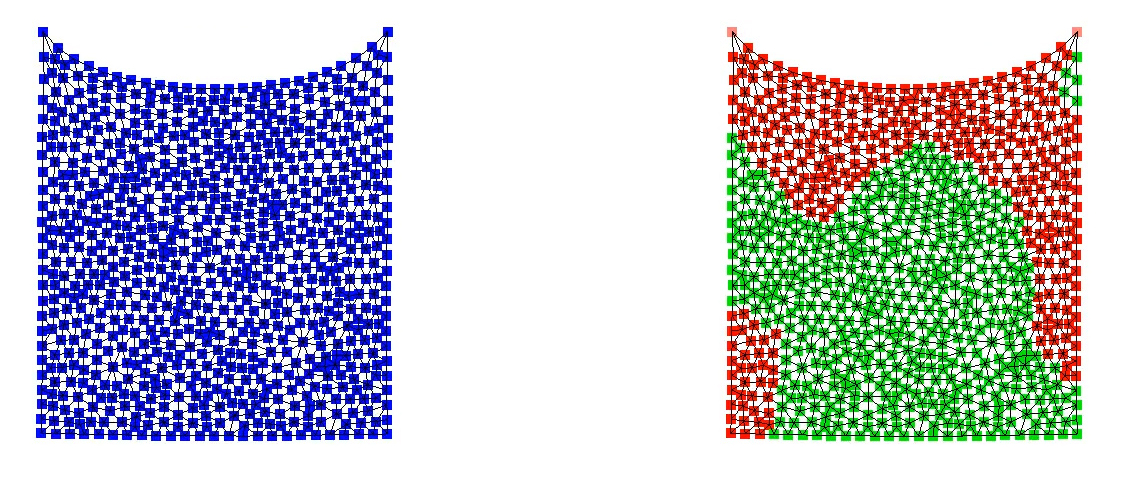
\includegraphics[width=0.8\linewidth]{images/arps-vriphys2013/Square3.jpg}
  \caption[ARPS: ARPS cloth simulation]{\label{fig:clothARPS} Hanging cloth. Left: traditional implicit simulation. Right: implicit ARPS simulation with a varying set of active and inactive particles. }
\end{figure}
Table~\ref{tab:clothePerf} shows performances we achieved with our hybrid solver.
As soon as a large number of particles become inactive the simulation is explicitly integrated and interesting speedup can raise.
\newline
However, while smoothly varying external forces are well handled by our simulator, we noticed instabilities when interacting strongly with the model.
They seem to occur during the transition between the transitive and the full-dynamics states.
A more thorough study of the influence of the transition function $\rho$ on the stability of the system would be necessary to come up with robust implicit ARPS simulations.
 This transition should be really well taken to avoid any instabilities.

\section{Implementation} 
\label{sec:arps_implementation}

\subsection{ Parameters }
ARPS use two parameters, $\epsilon^{r}$ and $\epsilon^{f}$ of Equation~\ref{eq:restrainingfunction}.
The main goal of ARPS in computer graphics is to save time when nothing happens.
So we generally want a low $\epsilon^{r}$ not to miss interesting movements.
When sudden movements occur, we want a normal reaction, so we want the inactive particles to quickly become active.
This requires a short transition, \textit{i.e.} $\epsilon^{f}$ close enough to $\epsilon^{r}$.
However, due to discrete time integration, a short transition may be stepped over, or not enough sampled, which may result in instabilities.
Currently we manually set the parameters, and defer the automatic tuning to future work.
In table \ref{tab:parameters} we refer the thresholds used in our simulations.
\begin{table}[htb]
    \centering
    \begin{tabular}{|c|c|c|c|} \hline
                & $\epsilon^{r}$    & $\epsilon^{f}$ & Tolerance \\ \hline
        SPH     &   1-e6            & 2-e5          & 8e-5 \\ \hline
        Cloth  &   0.05            & 1             & 1e-4 \\ \hline
\end{tabular}
    \caption[ARPS: Parameters for ARPS solver]{\label{tab:parameters} ARPS thresholds for SPH and Cloth simulation}
\end{table}

\subsection{Linear solver}
A linear equation solver is necessary in implicit integration, as presented in Section~\ref{sec:arps_implicit}.
In contrast with most formulations, implicit ARPS generally results in an unsymmetrical equation matrix, due to the matrix products in eq.(\ref{eq:arpsLinearSystem}).
We currently use a sparse LU solver from umfpack library, but it would be interesting to try a Conjugate Gradient method for unsymmetrical matrices to control the computation time, as it is usually done in implicit integration.

%-------------------------------------------------------------------------
\subsection{Choice of the restraining function and criterion}
In ARPS the restraining function is a $5^{th}$-order spline.
The spline directly depends on particle kinetic energy which is the \emph{restraining} criterion.
The implicit solver involves second derivatives of the restraining function, which may have large values, leading to instabilities.
We found that controlling the state of the particles based on momenta norm rather than kinetic energies seems to mitigate this and lead to more stable simulations.
We plan to investigate this issue in future work.


%-------------------------------------------------------------------------
\section{Discussion and concluding remarks} 
\label{sec:arps_discussion}
We have shown that ARPS, a new, simple approach to adaptive simulation, can effectively be applied to Computer Graphics, and we have demonstrated two specific applications.
The most successful one is the SPH simulation, for which we have obtained significant speedups with only minor changes to the original simulation method.
In the case of stiff material, we have obtained promising results for implicit integration, and we will address stability issues in future work, starting with a careful study of the restraining function.

Another interesting avenue is to employ non-physically-based transition criteria. The current one, based on kinetic energy, is well adapted to molecular dynamics simulation. In Computer Graphics, however, we are more interested in visual results. In future work, we thus plan to investigate the tuning of the transition thresholds based on visibility or distance to the camera, to even more focus the computational power where it most contributes to the quality of the result.
%\chapter{Detailed cutting of thin deformable models with sparse sampling}
\label{chap:cutting}

\begin{figure}[t]
\centering
\begin{subfigure}[b]{0.45\linewidth}
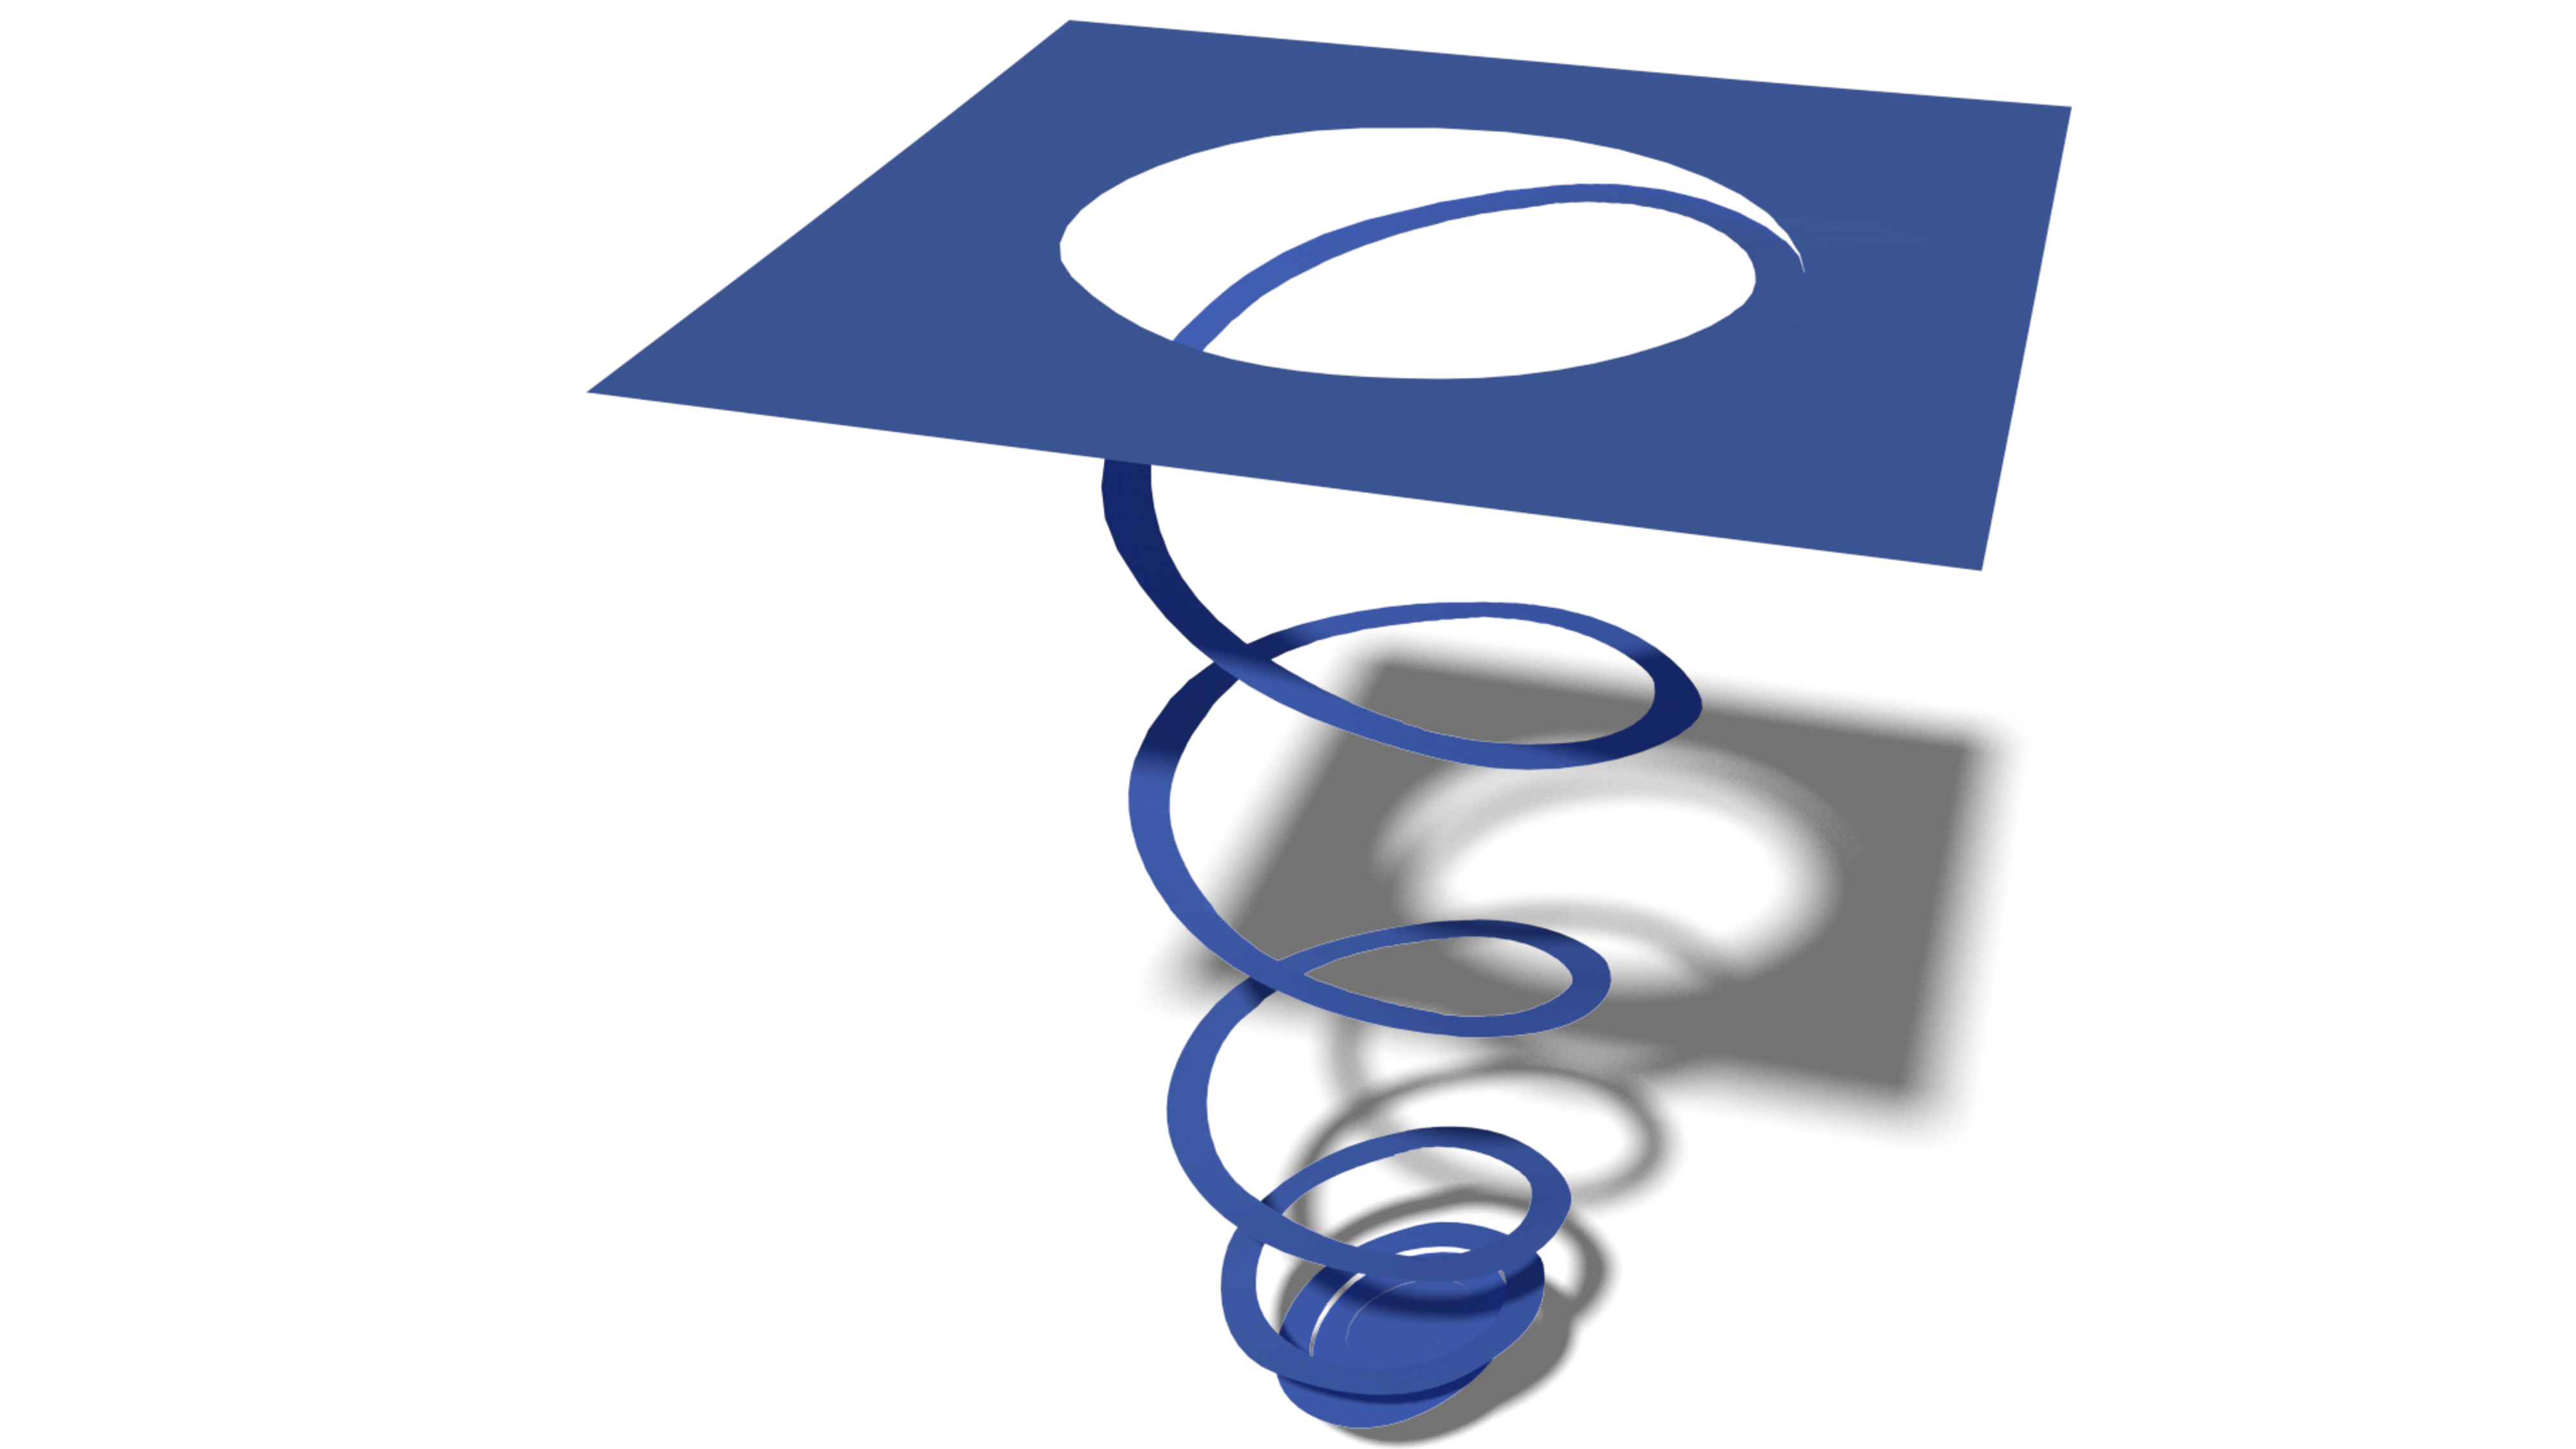
\includegraphics[width=\linewidth]{images/cutting-mig2015/Spiral2.pdf}
\caption{\label{fig:spiral}}
\end{subfigure}
\hfill
\begin{subfigure}[b]{0.45\linewidth}
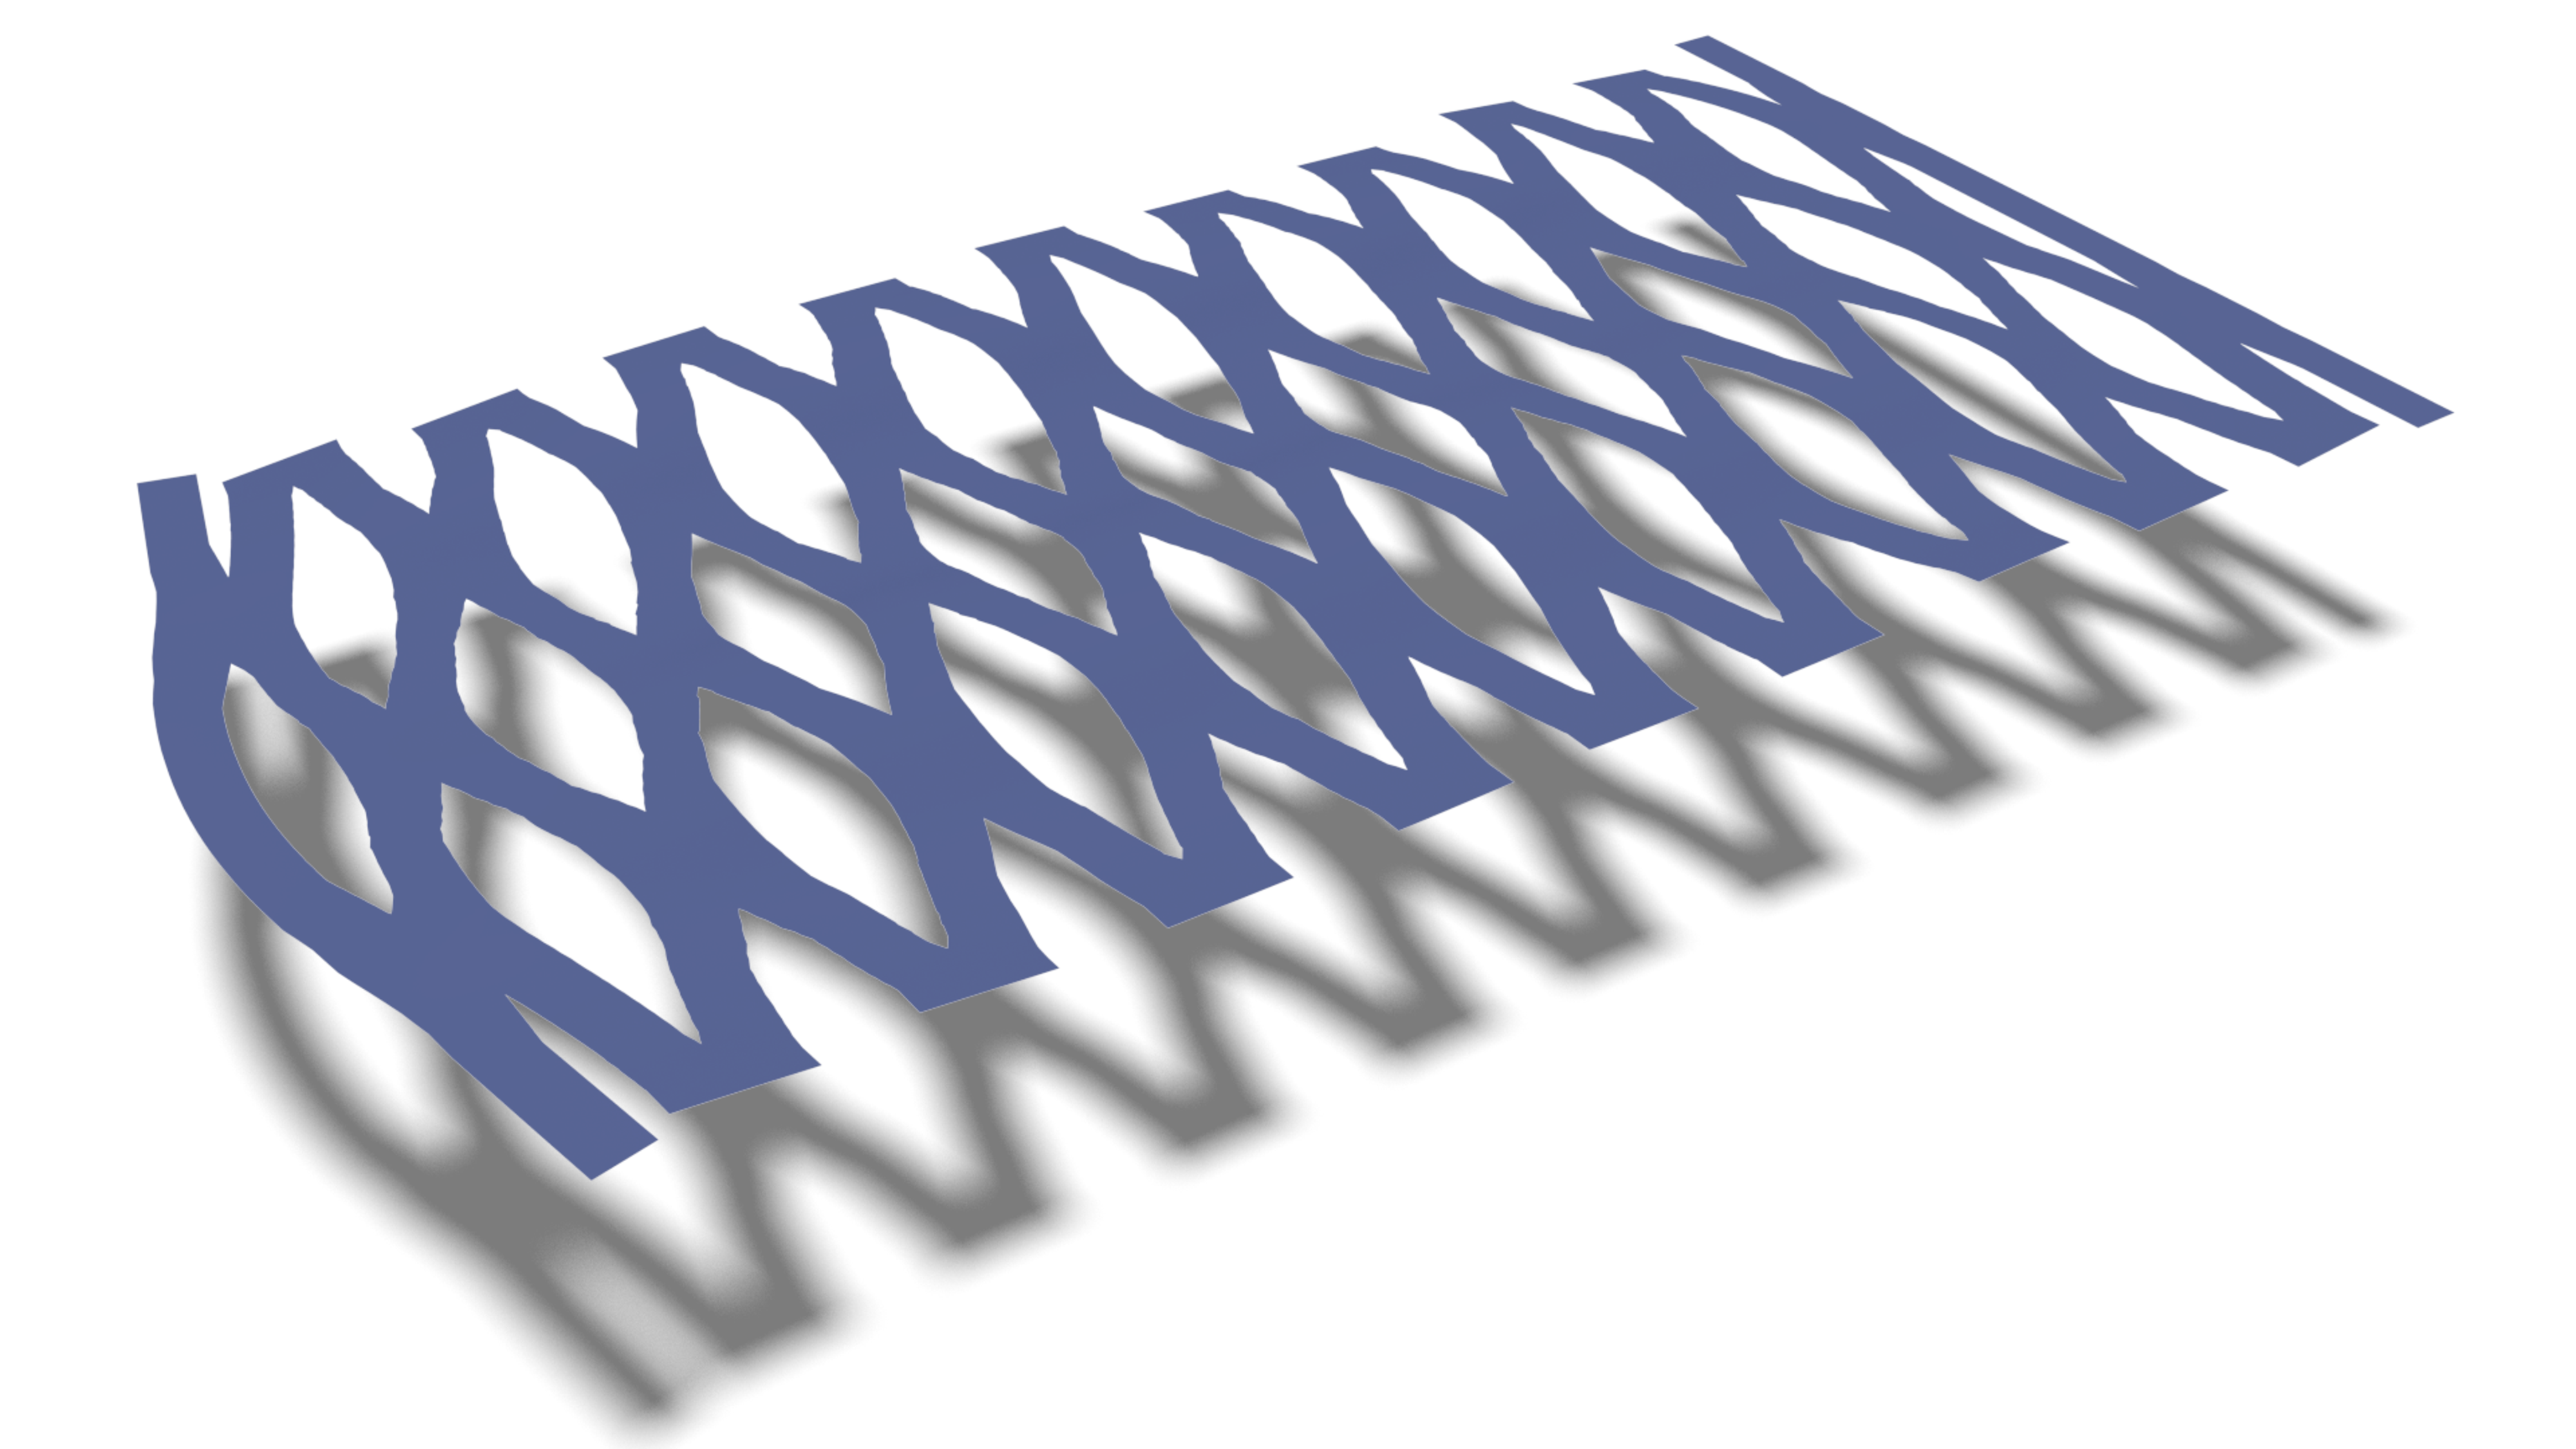
\includegraphics[width=\linewidth]{images/cutting-mig2015/Kirigami.pdf}
\caption{\label{fig:kirigami}}
\end{subfigure}
\caption[Frame-based cutting: Spiral and Kirigami cutting examples]{\label{fig:Cutting_Teaser} Progressive cutting of a spiral using only five control frames (a). Simulating complex deformations resulting from Kirigami cutting (b).}
\end{figure}

%%%%%%%%%%%%%%%%%%%%%%%%%%%%%%%%%%%%%%%%%%%%%%%%

%In this paper we propose a method for the interactive detailed cutting of deformable thin sheets. Our method builds on the ability of frame-based simulation to solve for dynamics using very few control frames while embedding highly detailed geometry - here an adaptive mesh that accurately represents the cut boundaries.
%Our solution relies on a non-manifold grid to compute shape functions that faithfully adapt to the topological changes occurring while cutting.  New frames are dynamically inserted to describe new regions. We provide incremental mechanisms for updating simulation data, enabling us to achieve interactive rates. We illustrate our method with examples inspired by the traditional Kirigami artform.

%%%%%%%%%%%%%%%%%%%%%%%%%%%%%%%%%%%%%%%%%%%%%%%%%%%%%%%%%%%%%%%%
%                       INTRODUCTION
%%%%%%%%%%%%%%%%%%%%%%%%%%%%%%%%%%%%%%%%%%%%%%%%%%%%%%%%%%%%%%%%
%\section{Introduction}
%Over the last three decades, physics-based animation methods have been proposed to simulate a wide range of phenomena. Substantial progress has been achieved in terms of efficiency and realism.  
%As a result, physics-based animation has found applications in film, games, craft, teaching, and training.
%\\ \\
Combining interactive user actions and detailed convincing animations is crucial for user experience in simulation and games. Unfortunately, computational contraints limit the 
fidelity that can be achieved with physics-based animation
in interactive simulations. Often, the simulated objects lack detail compared to the rest of the virtual environment.
Furthermore, operations that modify the structure of the simulated objects, such as cutting, 
maybe incompatible with faster simulation methods.
When not prohibited, the latter generally exhibit strong limitations. Indeed, the level of sampling of a physically-based model usually depends on geometric complexity. Detailed cuts result in an increase of the sampling which directly impacts the performance. In practice, the number of samples is limited to ensure real-time performance. This limitation quickly prevents the user from applying detailed cuts.  
\\ \\
In this chapter, we address the issue of enabling detailed cuts at interactive rates in  thin sheets of deformable materials. Our method is able to capture detailed cuts while using a relatively low number of control nodes for the physically-based model.
Our approach to decoupling the samplings of the physical geometric models, is to use a mesh-less simulation method called the frame-based model \cite{Gilles2011}. In this method, the deformation field induced by animated frames is applied to the geometric model using skinning weights. As each frame can cover a large, detailed shaped region of the geometric mesh, only a few of them are typically required.
\\ \\
To achieve user-driven cuts in a frame-based simulation, we allow cuts to be performed on the underlying mesh.
We build a non-manifold grid that keeps track of the mesh topology at the simulation level, and allows us to incrementally adapt the frames regions of influence in order to  represent the cut.
Although remaining low, the number of frame node does increase during a cut. In particular, when a model is cut apart, at least one frame is needed to represent each disconnected component. 
Therefore, we detect crucial cutting events, enabling us to automatically insert new frames when and where they are needed.
In order to reduce computations, we exploit the locality of the ongoing cutting gesture to incrementally update all the data used for the simulation.
\\ \\
Our contributions includes:
\begin{itemize}
\item The building of a non-manifold grid to compute shape functions that faithfully represent the  complex topology of the visual mesh while keeping a low number of control nodes.
\item The dynamic re-sampling of new frames into disconnected parts.
\item The incremental update of the simulation data that were concerned by the cut.
\end{itemize}
Our method can be used to simulate a wide variety of objects, such as stretchable cloth or pieces of paper. It features a very low number of frame nodes, high resolution mesh embedding, numerous and detailed cuts. Performance ranges from interactive to offline depending on the desired accuracy and complexity of the cuts.

\begin{figure*}[!ht]
\centering
\begin{subfigure}[c]{0.18\linewidth}
\centering
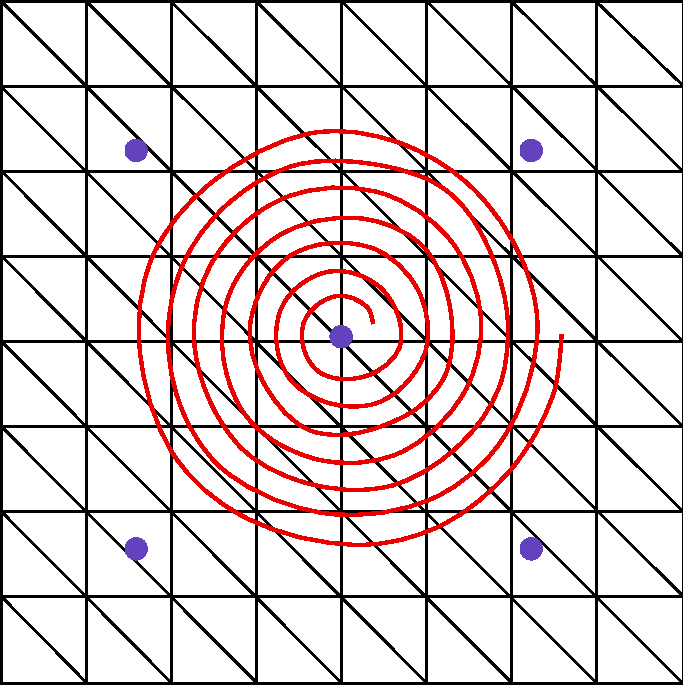
\includegraphics[width=\linewidth]{images/cutting-mig2015/spiral_mesh.pdf}
\caption{\label{fig:spiralMesh}}
\end{subfigure}
\hspace{1.5cm}
\begin{subfigure}[c]{0.68\linewidth}
\centering

\includegraphics[width=\linewidth]{images/cutting-mig2015/sfRender_ff/weightShow.pdf}
\caption{\label{fig:weightShow}}
\end{subfigure}
\caption[Frame-based cutting: Comparison of shape functions]{\label{fig:spiralWeight}
Comparison between shape functions computed on a uniform grid and on a non-manifold grid. (a) The underlying mesh (black lines) is cut by spiral (red line) and sampled with five control frames (blue circle). (b) The shape functions for each of the frame with a uniform grid (top row) and with a non-manifold grid (bottom row). Values range from $1$ to $0$ and are respectively depicted from red to blue. We can observe that shape functions computed on the non-manifold grid strictly preserve the details and topology of the underlying mesh.}
\end{figure*}
%%%%%%%%%%%%%%%%%%%%%%%%%%%%%%%%%%%%%%%%%%%%%%%%%%%%%%%%%%%%%%%%
%                       RELATED WORK
%%%%%%%%%%%%%%%%%%%%%%%%%%%%%%%%%%%%%%%%%%%%%%%%%%%%%%%%%%%%%%%%
\section{Related work on cutting and fracture}

Cutting and fracture are both fascinating behaviors which can be simulated separately. In fracture, stress measurements predict how the material breaks. In cutting, the interaction with a tool define the cut path. For more details about cutting we refer the reader to the recent survey of Wu et al. \cite{Wu2015}. Our review focuses on the modeling of topological changes in deformable models.

A first possibility consists in using the same model for physics simulation and visualization. Topological changes are then mostly modeled by remeshing operations. Simple and fast remeshing techniques such as element deletion or element splitting were proposed. The latter was used in the first simulation of brittle and ductile materials~\cite{OBrien1999}, \cite{OBrien2002}. 
 Methods that preserve element quality by local and global remeshing have also been developed. They recently lead to stunning results in the simulation of multi-layered paper tearing~\cite{Busaryev2013} and sheets tearing \cite{Pfaff2014}. 
These methods cause the number of simulation nodes to vary over the course of a simulation, and this variation can be problematic in a realtime game context.  By limiting the
scope of remeshing predictable realtime performance can be achieved~\cite{Parker2009}.
An alternative to remeshing is to enrich elements with additional basis so that discontinuities can be represented. This is the core idea of the eXtended Finite Element Method (XFEM). It was successfully applied for offline cutting of discrete shells \cite{Kaufmann2009}.

A second possibility is to separate the visual model from the physics model, this is known as embedding. Numerous embedding techniques have been proposed. The virtual node method \cite{Molino2004} embeds ill-shaped elements that arise after remeshing inside of well-shaped elements. This allows to robustly simulate detailed cuts \cite{Wang2014}. However, the number of nodes increases substantially with the complexity of the cut. To reduce it, hierarchical methods were proposed and real-time cutting in medical applications has been achieved using composite finite element method \cite{Wu2011}. Still, the number of nodes grows quickly with the number of cuts and remains limited to ensure interactive frame rate. Meshless methods avoid the problem of element quality. However, boundary and discontinuities require extra effort to be sharply represented. \cite{Pauly2005} proposed to use visibility criterion to perform fracture. \cite{Steinemann2009} used the visual model as a visibility graph to define nodes connectivity. Both methods rely on a dense sampling near the surface of the model and quickly impact performances as the number  and the detail of cuts increases. There also have some work to carry complex materials \cite{Nesme2009} and thin shells \cite{Remillard2013} in hexahedra elements.

Embedding techniques have inspired our work. They allow interesting trade-off and show impressive cutting and fracture simulations. However, the relation between the resolution of the physical model and the visualization model remains very strong. Complex cuts result in a fast increase of the number of nodes. We want to reduce this connexion as much as possible. Complex topologies could be simulated with a very low number of nodes. Then, interactivity and intuitive control would be at hand.

Few models have been proposed that simulate detailed deformable objects using a low number of nodes. Subspace simulations \cite{Barbic:2005:RTSI} compute a low basis of deformation modes in order to achieve real-time performance on detailed models. However, the low-basis is acquired after heavy precomputations. Interactive scenario could not handle the recomputation of the basis at each topological change. More recently, \cite{Gilles2011} and \cite{Faure2011} proposed a physics-based skinning technique, called the frame-based method. Highly detailed meshes can be embedded in very coarse simulations. The control nodes are affine frames and the deformation field is described by a linear blend skinning. Classical continuum mechanics is then used to solve for the dynamics. Skinning weights, also called shape functions, are built on linear interpolation using discrete voronoi regions. For each frame, they can represent a large region of influence with complex shape. Other advantages are discussed in \cite{Faure2011}. Unfortunately, the current frame-based method does not allow the shape functions to reflect the topological changes of the embedded mesh.

\section{Overview}

The goal of this work is to enable interactive detailed cutting of deformable thin sheets. The frame-based method exhibits some of the key features we are looking for: a very low number of nodes and a tunable separation between visual and physical models.  We build on this framework and extend it to handle topological changes.

To transfer the cuts from the mesh to the frames, we continuously adapt the shape functions to the evolving mesh topology. This allows us to keep a constant number of nodes as long as there are no disconnected parts. In \cite{Faure2011}, the shape functions are computed on a uniform grid. The structure is simple and efficient. However, discontinuities that can be represented are very limited and strongly connected to the grid resolution. Instead, we build a non-manifold grid to compute topology-preserving shape functions (see Figure \ref{fig:spiralWeight}). The main idea is that cut cells are duplicated and store different connectivities. Therefore, grid resolution depends much less on the mesh topology while keeping all topological informations.

We detail the computation of the shape functions, motivate the use of a non-manifold grid and explain how to build it (Section \ref{sec:adaptivesf}). When several parts are disconnected, we need to make sure that they contain control frames. We present a simple method to detect those regions and re-sample them (Section \ref{sec:resampling}). Even with such a low resolution physics model, it would be overkilling to update the whole system at each cut. Fortunately, cutting is often a local event. We leverage this fact and propose simple strategies to incrementally update the different components of the simulation (Section \ref{sec:incremental}). We illustrate our method in different scenarios (Section \ref{sec:results}) and discuss limitations and future work (Section \ref{sec:cutting_conclusion}). We summarize our simulation loop in Algorithm~\ref{alg:simulationLoop} and detail our remeshing algorithm in appendix~\ref{appendix:remeshing}.

\begin{algorithm}[!h]
\caption[Frame-based cutting: Simulation loop]{\label{alg:simulationLoop}Simulation loop}
\begin{algorithmic}[0]
\For{each time step}
	\State perform a frame-based simulation step
	\State split the mesh along the cut
	\State embed the mesh in a non-manifold grid
	\State add new frames if required
	\State add new samples (collision, integration) if required
	\State compute shape functions on the grid
	\State incrementally update the samples
\EndFor
\end{algorithmic}
\end{algorithm}

%%%%%%%%%%%%%%%%%%%%%%%%%%%%%%%%%%%%%%%%%%%%%%%%%%%%%%%%%%%%%%%%
%                      WEIGHT COMPUTATION / GRID
%%%%%%%%%%%%%%%%%%%%%%%%%%%%%%%%%%%%%%%%%%%%%%%%%%%%%%%%%%%%%%%%
\section{Adaptive shape functions} \label{sec:adaptivesf}

In this section, we first summarize how Voronoi shape functions are traditionally computed. Then we detail why a non-manifold grid is necessary, how to build it and how to use it to compute the shape functions on complex topology.

%%%%%%%%%%%%%%%%%%%%%%%%%%%%%%%%%%%%%%%%%%%%%%%%%%%%%%%%%%%%%%%%
%                      SHAPEFUNCTION
%%%%%%%%%%%%%%%%%%%%%%%%%%%%%%%%%%%%%%%%%%%%%%%%%%%%%%%%%%%%%%%%
\subsection{Voronoi shape function}
\begin{figure*}[!ht]
\centering
\begin{subfigure}[b]{0.20\linewidth}
\centering

\includegraphics[width=\linewidth]{images/cutting-mig2015/buildSF_1.pdf}
\caption{\label{fig:buildSF1}}
\end{subfigure}
\hspace{2cm}
\begin{subfigure}[b]{0.20\linewidth}
\centering
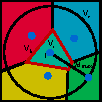
\includegraphics[width=\linewidth]{images/cutting-mig2015/buildSF_2.pdf}
\caption{\label{fig:buildSF2}}
\end{subfigure}
\hspace{2cm}
\begin{subfigure}[b]{0.20\linewidth}
\centering
\includegraphics[width=\linewidth]{images/cutting-mig2015/buildSF_3.pdf}
\caption{\label{fig:buildSF3}}
\end{subfigure}
\caption[Frame-based cutting: Voronoi shapefunction computation]{\label{fig:shapefunctionconstruction}
Illustrations of Voronoi shape function computation. (a) Starting from samples (blue circles), we build a Voronoi diagram using Dijkstra's shortest path algorithm. (b) Then, for each frame and its region $V_{i}$, we compute the maximum distance $d_{max}$ to its Voronoi boundary $V_{b}$. We extend $V_{i}$ to twice $d_{max}$ which gives $V_{e}$. (c) Finally for each grid cell $j$ in $V_{e}$ we linearly interpolate using distance to the frame position and distance to $V_{b}$.}
\end{figure*}

Let $w_{i}(x) : \Omega \rightarrow \mathcal{R}$ be the shape function for the $i$-th control frame, where $\Omega$ represents the domain. Starting from the Voronoi partition $V$ of the set of control frames, we can independently compute $w_{i}$ for each frame.

First, we compute the maximal distance $d_{max}$ from the control node to its Voronoi boundary $V_{b}$. Then we extend its Voronoi region $V_{i}$ to twice $d_{max}$. This gives a new region $V_{e}$ which describes the final boundary of the shape function. Now, we can compute $w_{i}$ inside $V_{e}$. We set $w_{i}$ to be $1$ at the frame position, $0$ at the others and $0.5$ on $V_{b}$. Finally, we linearly interpolate $w_{i}$ between $V_{b}$, the frame position and the boundary of $V_{e}$. We detail the interpolation in Algorithm~ \ref{alg:shapefunctioncomputation} and in Figure~ \ref{fig:shapefunctionconstruction}.

In practice, Voronoi diagram is computed using Dijkstra's shortest path algorithm on a grid in order to preserve geodesic distances. For each frame, the shape function is computed on the whole grid. As the grid resolution can be quite coarse, this is particularly fast. Negative values are clamped and weights are normalized to form a partition of unity. Then least-square approximation is performed to evaluate the shape function and its derivatives at specific position.

\begin{algorithm}[h]
\caption[Frame-based cutting: Shapefunction computation]{\label{alg:shapefunctioncomputation}Shapefunction computation}
\begin{algorithmic}[1]
\Procedure{Compute$\_$Shapefunction}{}
\For{each frame $i$}
	\State $V_{i} \gets$ Voronoi region of $i$
	\State $V_{b} \gets$ boundary of $V_{i}$	
	\State $d_{max} \gets$ maximum distance to $V_{i}$ boundary
	\State $V_{e} \gets$ extend $V_{i}$ to $2.0 \times d_{max}$
	\LineComment{dist($A$,$B$) is the geodesic distance between $A$ and $B$}
	\For{each grid cell $j$ in $V_{e}$}
	\If{$j$ is inside $V_{i}$}
	\State $\displaystyle w_{i}(j) = 0.5\left(1 + \frac{dist(j,V_{b})}{dist(j,V_{b})+dist(j,i)}\right)$
	\ElsIf{$j$ is inside $V_{e}$}
		\State $\displaystyle w_{i}(j) = 0.5\left(1 - \frac{dist(j,V_{b})}{dist(j,i)-dist(j,V_{b})}\right)$
	\EndIf
	\EndFor
\EndFor
\EndProcedure
\end{algorithmic}
\end{algorithm}

Voronoi shape functions were designed in order to respect key properties that are particularly useful for physics-based animation \cite{Faure2011} . First, they respect the Kronecker property, i.e $w_{i}(x) = \delta_{i}(x)$ where $w_{i}(x)$ is the shape function of node $i$, $x$ is a spatial position and $\delta_{i}$ is Dirac function. Second, they form a partition of unity, i.e $\sum_{i}w_{i}(x) = 1$. Third, they are built to be as linear as possible in order to produce uniform deformations. Finally, they can easily be biased by material properties in order to represent heterogeneous material.

%In the extension of the frame-based method \cite{Faure2011}, they propose to use Voronoi shape functions. In this method, the region of influence of each frame is defined by an extension of its voronoi region. Weights are linearly interpolated between the position of the frame and the boundary of the initial voronoi region and they are extrapolated between the boundary of the initial voronoi and the boundary of the extended voronoi. In their paper, the voronoi diagrams are computed on a discrete grid with a 8 neighbor connectivity using a Dijkstra algorithm. Weights and weight derivatives are then interpolated to specific sample positions such as mesh vertices or integration points or collision points. Weights are ensured to be linear along shortest path. This method allows to biase the distance computation by a material map in order to build weights that can represent heterogenous material. In our method we use the same shape functions in order to represent large regions and hetergenous materials. However we need to adapt the shape functions along the simulation to take into accounts the cuts.
%Shape functions describe the influence region of each node. In linear finite element methods, this region is clearly delimited by the elements that surrounds each vertex. Thus topology is naturally represented by the mesh itself. In mesh-less methods, 
%Each vertex influence 
%barycentric linear shape functions are used in triangular and tetrahedral meshes. They naturally represent the topology of the mesh and produce uniform deformations. In mesh-less methods, each node 
%The design of shape functions for skinning deformation is an active topic of research. Several key features have been identified in order to produce plausible deformations.
%Three key features that ensure plausible deformations have been identified. The first one is that the shape function should decrease with respect to the distance from the corresponding control node. The second one is that it should be as linear as possible in order to produce uniform deformations. Finally, it should respect the Kronecker property in order to provide easy  manipulations.
%Usually, three key features should be preser
%They should  Generally, the function decreases from $1$ to $0$ from the node position 
%Linear shape functions ensure that the material deform uniformly with the frame motions. 
%Usually, we want the region attached to a node to deform uniformly with it. Therefore we use linear weights
%the region of influence of each control frame
%The design of skinning weights is an active topic of research.
%Skinning weights describe the region of influence of the control frames and the type of influence. Generally we want the space to deform uniformly with the frames and so we use linear weights. When the region of a node is a simple shape such as a set of triangles or a quads, one can use well known weights such as barycentric or bilinear weights. However, when we do not want to describe the deformation field using a specific geometry, it is much more challenging to design shape functions. Most of the meshless methods use overlapping spline kernel with local support to describe the deformation field. Unfortunately this requires relatively dense sampling to cover the whole region. Nevertheless, both methods use local shape functions and assume that the number of nodes is important. In procedural animation, design of skinning weights is an active topic of research. The goal is to design weight that can cover regions of different sizes, while respecting the topology in order to provide intuitive control of a shape. An important step was achieved by the work of \cite{Joshi2007} where they propose to use harmonic coordinates. Those skinning weights provide control over large regions while keeping the coherency of the topology. Unfortunately, those weights are highly nonlinear and results in unconvining behavior in physics-based simulation. 

\subsection{Non-manifold grid}

As mentionned above, in \cite{Faure2011}, shape functions are computed on a uniform grid using Dijktra's shortest path algorithm to compute geodesic distance. Starting from a uniform grid with a 8-neighbor connectivity, we could reflect topological change by changing the connectivity of the cut cells. Then, when we re-compute shape functions, the topology would automatically be taken into account as we use geodesic distance. 

Unfortunately, this strategy is very limited for uniform grid and would only work in simple cases. For instance, several cuts that intersect or that create disconnected components inside one cell could not be represented. Even without cut, small gaps that lie inside one cell could not be correctly represented. Geodesic distances would be false and the object would behave as if there were no cuts or gaps. Augmenting the resolution would not solve the problem. We would fight the same issue as previous methods. Our grid resolution would be highly dependent on the complexity of the topology and the geometry of the object. It would directly impact performances.

\begin{figure*}[t]
\centering
\begin{subfigure}[b]{0.20\linewidth}
\centering
\includegraphics[width=\linewidth]{images/cutting-mig2015/connectivity.pdf}
\caption{\label{fig:connectivity}}
\end{subfigure}
\hfill
\begin{subfigure}[b]{0.30\linewidth}
\centering
\includegraphics[width=\linewidth]{images/cutting-mig2015/simple_cut.pdf}
\caption{\label{fig:simplecut}}
\end{subfigure}
\hfill
\begin{subfigure}[b]{0.40\linewidth}
\centering
\includegraphics[width=\linewidth]{images/cutting-mig2015/little_pieces.pdf}
\caption{\label{fig:littlePieces}}
\end{subfigure}
%\hfill
%\begin{subfigure}[b]{0.24\linewidth}
%\centering
%\includegraphics[width=\linewidth]{images/cutting-mig2015/multi_cut.pdf}
%\caption{\label{fig:multicut}}
%\end{subfigure}
\caption[Frame-based cutting: Non-manifold grid illustration]{\label{fig:nonmanifoldgridillustration}
Illustrations of different possibilities for a non-manifold cell with eight connectivity (a). In (b), the cell is simply cut into two cells. Each duplicate of the cut cell has a specific connectivity that represent the cut topology. In (c), multiple disconnected components can be contained inside one cell. The cell is duplicated four times. Three of the duplicates have no connectivity. However they can embed complex geometry and then be simulated by adding new frames for each of the component. The fourth duplicate keeps its eight neighbors and remains independent from the three other.}
\end{figure*}

We want each grid cell to be able to represent  the connectivities of the different disconnected components that lie in the cell. To do so, each cut cell is duplicated as many times as it contains disconnected parts. Each duplicate has a specific connectivity built from the material connectivity. This results in a data structure called \emph{non-manifold grid} (see Figure \ref{fig:nonmanifoldgridillustration}).

\begin{figure*}[t]
\centering
\begin{subfigure}[b]{0.20\linewidth}
\centering
\includegraphics[width=\linewidth]{images/cutting-mig2015/buildNMG_1.pdf}
\caption{\label{fig:buildNMG1}}
\end{subfigure}
\hfill
\begin{subfigure}[b]{0.20\linewidth}
\centering
\includegraphics[width=\linewidth]{images/cutting-mig2015/buildNMG_2.pdf}
\caption{\label{fig:buildNMG2}}
\end{subfigure}
\hfill
\begin{subfigure}[b]{0.20\linewidth}
\centering
\includegraphics[width=\linewidth]{images/cutting-mig2015/buildNMG_3.pdf}
\caption{\label{fig:buildNMG3}}
\end{subfigure}
\hfill
\begin{subfigure}[b]{0.20\linewidth}
\centering
\includegraphics[width=\linewidth]{images/cutting-mig2015/buildNMG_4.pdf}
\caption{\label{fig:buildNMG4}}
\end{subfigure}
\caption[Frame-based cutting: Non-manifold grid building]{\label{fig:nonmanifoldgridbuilding}
We describe the building of the non-manifold grid for the center cell of the grid. (a) The mesh is embedded in a uniform grid. (b) First, we store the overlapping geometry in the cell. (c) Then we detect disconnected parts using a flood fill algorithm. (d) Finally the cell is duplicated. For each duplicate, we look for other duplicates that share geometry and establish its connectivity.}
\end{figure*}

Non-manifold grids are used by many other cutting methods to embed fine geometric details in coarse finite element simulations. However, we make a completely different use of it. Instead of duplicating control nodes as the cells are cut, thereby increasing their number and the computation time, we use the grid to adapt the shape functions to the evolving topology of the mesh. Most of the time, the number of nodes can remain constant while representing detailed geometry and multiple cuts.

There are several ways to compute this non-manifold grid. In our method, we start by embedding the mesh in a uniform grid. Mesh elements that overlap a grid cell are detected using intersections tests and are assigned to it. Then, for each grid cell, we use a flood fill algorithm to detect the disconnected parts of the mesh. This informs about how many duplicates need to be created for the cell. Finally, for each duplicate we establish its connectivity by comparing its geometry with the geometry of the neighbor cells duplicates. We summarize our method in Algorithm~\ref{alg:nonmanifoldbuilding} and illustrate the main steps in Figure~\ref{fig:nonmanifoldgridbuilding}.

\begin{algorithm}[!hb]
\caption[Frame-based cutting: Non-manifold grid building]{\label{alg:nonmanifoldbuilding}Non-manifold grid building}
\begin{algorithmic}[1]
\Procedure{Build$\_$Non$\_$Manifold$\_$Grid}{grid $G$, mesh $M$}
\State \textsc{Build$\_$Grid$\_$Geometry}($G$,$M$)
\State \textsc{Duplicate$\_$Grid$\_$Cell}($G$)
\State \textsc{Build$\_$Grid$\_$Connectivity}($G$)
\EndProcedure
\State
\Procedure{Build$\_$Grid$\_$Geometry}{grid $G$, mesh $M$}
\For{each cell $i$ of $G$}
\State Store overlapping element of $M$
\EndFor
\EndProcedure
\State
\Procedure{Duplicate$\_$Grid$\_$Cell}{grid $G$, mesh $M$}
\For{each cell $i$ of $G$}
\State $C \gets $ disconnected component of $M$ in $i$
\For{each component j of $C$}
	\State Duplicate the cell $i$
	\State Store $j$ in the duplicate
\EndFor
\EndFor
\EndProcedure
\State
\Procedure{Build$\_$Grid$\_$Connectivity}{grid $G$}
\For{each cell $i$ of $G$}
\State $N \gets $ neighbor cells of $i$
\For{each duplicate $j$ of $i$}
\For{each duplicate $k$ in $N$}
\If{$j$ and $k$ shares geometry}
\State Create a link between $j$ and $k$ 
\EndIf
\EndFor
\EndFor
\EndFor
\EndProcedure
\end{algorithmic}
\end{algorithm}

%%%%%%%%%%%%%%%%%%%%%%%%%%%%%%%%%%%%%%%%%%%%%%%%%%%%%%%%%%%%%%%%
%                      FRAME RESAMPLING
%%%%%%%%%%%%%%%%%%%%%%%%%%%%%%%%%%%%%%%%%%%%%%%%%%%%%%%%%%%%%%%%

\section{Frame re-sampling} \label{sec:resampling}
As long as no parts of the model are disconnected, our method allows to keep a constant number of control frames. However, when parts are disconnected, we need to sample it with at least one frame in order to simulate it. 

We start by detecting empty regions i.e lists of connected cells that are not influenced by any frame. This is done using a flood fill algorithm on the grid containing the shape functions values. These empty regions are then sampled using a farthest sampling algorithm. Finally, the samples are uniformly distributed by applying several Lloyd relaxation steps. For now, the number of frames which are sampled is user-defined but we would like to investigate for setting it automatically (see Section \ref{sec:cutting_conclusion}). 

As a cut progresses, it may happen that only one frame influences a large region. Then this region can only express affine motion. Depending on the material properties, the size and the shape of the region, this can result in unconvincing behaviours. For rigid materials this is not a problem but for soft material this can quickly become unrealistic. We propose a simple strategy to solve some of these cases. For each frame, we look for regions where the shape function value is above a user-defined threshold $w_{max}$. Then if the volume of the region is above a maximal volume threshold $v_{max}$, we uniformly re-sample the region. This strategy allows to detect large regions which are mostly influenced by only one frame and are the most likely to need re-sampling. For now, $w_{max}$ and $v_{max}$ are user-defined.

As regions of influence are very large, the popping artefacts induced by adding instantaneously one additional frame can be noticeable. In order to reduce them we propose a simple strategy. Once the position of the new frame in the undeformed, material space has been chosen, we use the previous deformation field to interpolate its new position, orientation and velocity.

%%%%%%%%%%%%%%%%%%%%%%%%%%%%%%%%%%%%%%%%%%%%%%%%%%%%%%%%%%%%%%%%
%                      INCREMENTAL UPDATE
%%%%%%%%%%%%%%%%%%%%%%%%%%%%%%%%%%%%%%%%%%%%%%%%%%%%%%%%%%%%%%%%
\section{Incremental update} \label{sec:incremental}

The domain and the shape functions continuously change during cutting. Therefore, all the simulation data that are related to the domain or the shape functions need to be updated at each time step a cut occurs. Fortunately, cutting is often a local phenomenon. We exploit this locality to incrementally update only what is necessary and therefore save substantial computational time.

In our case, there are several simulation components that need to be updated. The first of this component contains the integration points that compute deformation gradients and transfers internal forces to the control frames. Then there is the collision component, a simple set of points, that transfers external forces to the control frames. Finally, there is the mesh that we visualize whose vertices positions are interpolated from the frame positions. Each of this component can have its own resolution. Their data are computed from the control frames using interpolation. This layer-based organization allows to separate the resolutions of the physical simulation, the interactive model and the visual rendering to achieve a good trade-off between realism and performance.

In the following sections we describe the mechanisms we used to incrementally update the different components of the simulation.

\subsection{Re-sampling}
\label{sec:all_resampling}
As for the frames, we always need to have at least one collision node and one integration point inside each part of the model. Otherwise, we cannot compute deformations or interact with these parts of the model. Usually, there are much more collision nodes and integration points than frames. Instead of adding new points only when we detect new empty regions, we perform a few Lloyd relaxation steps at each time step to always keep a uniform sampling of the domain. In a progressive cut scenario, only a small number of samples will need to be updated at each time step and will result in an efficient incremental update. However, if disconnected parts are created from a cut, we apply the re-sampling strategy discussed in Section \ref{sec:resampling}. We detect the disconnected parts using a flood fill algorithm and uniformly re-sample them.

\subsection{Integration point update}
\label{sec:gausspointupdate}

Integrations points are used to compute deformation gradients and transfer internal forces to the frames. To do so, each integration point are interpreted as a small volume of the domain and carries a position, a region's volume and the volume moments. As soon as a cut occurs, the region's volume of integration points close to the cut will change and it becomes necessary to update these integration points. This can be easily done by storing an explicit description of the region of the integration point i.e a list of cells. If the cut goes through one of these cells then we update the integration point data.

\subsection{Local weights update} \label{sec:interpolation}

Weights and derivatives are interpolated from the grid to positions of the different samples : collision nodes, integration points and mesh vertices. At each cut, we need to update these values. In an interactive context, we cannot afford to perform interpolation for all these samples. Once again, we leverage the fact that a cut is very often a local event, sometimes progressive, and will impact only a small fraction of the different samples. Our idea is to perform incremental update of weights and derivatives by detecting the low number of samples that were impacted by the cut. At each time step, if a cut was performed, we compare the new shape functions with the previous ones and detect the grid cells which have been impacted by the cut. All the samples that are contained or are neighbors of these cells need to be updated. In the end, even if we have control frames that covers large regions of the domain compared to classical simulations, simulation data that need to be updated remains spatially local.
\begin{figure*}[ht]
\centering
\begin{subfigure}[b]{0.32\linewidth}
\centering
\includegraphics[width=\linewidth]{images/cutting-mig2015/Patchwork.pdf}
\caption{\label{fig:patchwork}}
\end{subfigure}
\hfill
\begin{subfigure}[b]{0.32\linewidth}
\centering
\includegraphics[width=\linewidth]{images/cutting-mig2015/FallingGuy.pdf}
\caption{\label{fig:fallingguy}}
\end{subfigure}
\hfill
\begin{subfigure}[b]{0.32\linewidth}
\centering
\includegraphics[width=\linewidth]{images/cutting-mig2015/Vortex.pdf}
\caption{\label{fig:vortex}}
\end{subfigure}
\caption[Frame-based cutting: Examples of detailed cutting]{\label{fig:result} (a) Several highly detailed shapes are cut in a deformable sheet. Each disconnected part is automatically re-sampled with additional control frames. (b) Simulation of a highly detailed cut that falls under gravity and remains attached to the main part by a thin piece of paper. (c) Two cuts intersect to form a vortex shape. This illustrates the abilities of the non-manifold grid to handle multiple intersecting cuts.}
\end{figure*}

\addtolength{\tabcolsep}{-1.5pt}
\begin{table*}[!ht]
\centering
\scalebox{0.63}
{
\begin{tabular}{l|c|cc|cc|c|c|ccc}
& & \multicolumn{2}{c|}{\#frame} & \multicolumn{2}{c|}{\#vertices} & & & \multicolumn{3}{c}{Lowest FPS}\\
Name & Grid Size & Initial & Final & Initial & Final & \#collision & \#integration & \begin{tabular}{c}Before \\ Cutting\end{tabular}  & \begin{tabular}{c}During \\ Cutting\end{tabular}  & \begin{tabular}{c}After \\ Cutting\end{tabular}  \\ \hline
Spiral (Fig. \ref{fig:spiral}) & $40 \times 40$ & $5$ & $5$ & $81$ & $2111$ & $200$ & $200$ & $60$ & $14.4$ & $60$\\ 
Kirigami (Fig. \ref{fig:kirigami}) & $68 \times 68$ & $47$ & $47$ & $4225$ & $7453$ & $600$ & $800$ & $11.3$ & $3.2$ & $10.9$\\ 
Patchwork (Fig. \ref{fig:patchwork}) & $50 \times 50$ & $5$ & $12$ & $4225$ & $8253$ & $200$ & $200$ & $60$ & $6.8$ & $45$\\
Vortex (Fig. \ref{fig:vortex}) & $68 \times 68$ & $5$ & $5$ & $4225$ & $4889$ & $200$ & $200$ & $45$ & $7.2$ & $35.7$\\
FallingGuy (Fig. \ref{fig:fallingguy}) & $100 \times 50$ & $10$ & $10$ & $289$ & $861$ & $500$ & $500$ & $60$ & $8.2$ & $60$\\
\end{tabular}
}
\caption[Frame-based cutting: Resolution \& timings]{\label{tab:performance} Resolution of the different components of the simulation and timings.}
\end{table*}

\addtolength{\tabcolsep}{1.5pt}

\begin{table*}[!ht]
\centering
\scalebox{0.7}
{
\begin{tabular}{l|ccccc}
& \multicolumn{4}{c}{Percentage of update for a cutting step} \\
Name & \%grid cell &\%shape function cell & \%vertices & \%collision nodes & \%integration points \\ \hline
Spiral (Fig. \ref{fig:spiralMesh}) & $0.07$ & $28.1$ & $61.5$ & $27.2$ & $41.3$\\
Kirigami (Fig. \ref{fig:kirigami}) & $1.06$ & $15.9$ & $17.8$ & $15.8$ & $20.3$\\
Patchwork (Fig. \ref{fig:patchwork}) & $0.02$ & $2.78$ & $4.33$ & $2.55$ & $7.15$\\
Vortex (Fig. \ref{fig:vortex}) & $0.08$ & $10.3$ & $12.8$ & $9.2$ & $24.2$\\
FallingGuy (Fig. \ref{fig:fallingguy}) & $0.09$ & $5.84$ & $11.4$ & $5.77$ & $14.9$\\
\end{tabular}
}
\caption[Frame-based cutting: Incremental update timings]{\label{tab:incrementalUpdate} Percentage of updated data in a cutting time step. We averaged the percentage for the whole cutting time. We notice that even if very few grid cell are affected, it implies important changes on the shape functions and the samples that are associated to these values.}
\end{table*}

%%%%%%%%%%%%%%%%%%%%%%%%%%%%%%%%%%%%%%%%%%%%%%%%%%%%%%%%%%%%%%%%
%                      RESULTS 
%%%%%%%%%%%%%%%%%%%%%%%%%%%%%%%%%%%%%%%%%%%%%%%%%%%%%%%%%%%%%%%%
\section{Results} \label{sec:results}

We illustrate our method in a variety of simulations where a piece of paper undergoes progressive scripted cuts. As we use several layers of samples (frames, collision nodes, integration points), choosing a good trade off between accuracy and performance is essential. In all the examples, we used the minimum number of samples we could without compromising visual results (see Table \ref{tab:performance}). Frame re-sampling was required to simulate disconnected parts. However it appears that no additional collision nodes or integration points were required. We can deduce that our relaxation strategy is sufficient to keep the object uniformly sampled along the simulation.

All our examples run at interactive frame rate during the whole simulation (see Table \ref{tab:performance}). Frame rates were collected on a twelve-core 3.20 GHz Intel Xeon CPU with 15.6 GB RAM. We highlight that our implementation is not optimized and there are still a lot of room for improvements that we did not have time to implement. Full animated results are shown in the accompanying video.

Figure \ref{fig:spiral} shows a long spiral cut in a sheet of paper simulated with only $5$ frames. The shape functions of the frames faithfully represent the cut as shown in Figure \ref{fig:spiralWeight}. 

To illustrate that our method can handle multiple cuts and still simulate complex deformations, the creation of a Kirigami is shown in Figure \ref{fig:kirigami}. $48$ cuts are performed and it only required $47$ frames and $400$ integration points to produce a plausible behavior.

Detailed cuts can be performed and separated components can be handled as shown in Figure \ref{fig:patchwork}. In a cloth sheet, we progressively cut bunny, teapot, dragon and armadillo shapes. Each time a new object is completely cut, it is automatically re-sampled with additional frames.

As we explained, the non-manifold grid can represent an arbitrary number of connectivity in one cell. This is particularly useful in order to represent intersecting cuts as shown in Figure \ref{fig:vortex}.

We noticed that even if a cut only concern a few grid cells, the number of data to re-compute is much more important. This comes from the fact that each frame can cover a large region and changes arising from a local cut can be important. Fortunately, our incremental update mechanisms allows to save numerous unnecessary computations as shown in Table \ref{tab:incrementalUpdate}. 

%%%%%%%%%%%%%%%%%%%%%%%%%%%%%%%%%%%%%%%%%%%%%%%%%%%%%%%%%%%%%%%%
%                      REMESHING
%%%%%%%%%%%%%%%%%%%%%%%%%%%%%%%%%%%%%%%%%%%%%%%%%%%%%%%%%%%%%%%%
\section{Remeshing} \label{appendix:remeshing}

As stated previously, the mesh is only used for visualization. Simulation robustness will not be determined by its elements' quality. Therefore we used an extremely simple remeshing algorithm. The input are the mesh and a polyline that represents the cut. We start by remeshing along the polyline so that the mesh  conforms with it. Then we duplicate the mesh vertices along this polyline to create the crack. The whole procedure is summarized in algorithm \ref{alg:remeshing} and illustrated in Figure \ref{fig:remeshing}. The remeshing part uses vertex insertion and edge split operations (see Figure \ref{fig:operations}). The splitting part only uses vertex split operation (see Figure \ref{fig:vertexSplitting}).

\begin{algorithm}[hp]
\caption[Frame-based cutting: Remeshing algorithm]{\label{alg:remeshing}Remeshing Algorithm}
\begin{algorithmic}[1]
\Procedure{Cut$\_$Along$\_$Segment}{Segment $S$, mesh $M$}
\State \textsc{Insert$\_$Segment}($S$, $M$)
\State $\tilde{P} \gets$ edges corresponding to $S$
\State \textsc{Split$\_$Along$\_$Polyline}($\tilde{P}$,$M$)
\EndProcedure
\State
\Procedure{Insert$\_$Segment}{Segment $S$, Mesh $M$}
\State $\tilde{S} \gets$ subdivide $S$ at intersection with $M$ edges
\For{each point $i$ of $\tilde{S}$}
\State $E \gets$ closest edge to $i$
\State $V \gets$ closest vertex to $i$
\State $F \gets$ closest triangle to $i$
\If{distance($E$,$i$)$<\epsilon_{edge}$}
\State Split $E$ at $i$
\ElsIf{distance($V$,$i$)$<\epsilon_{vertex}$}
\State Snap $i$ to $V$
\Else
\State Split $F$ at $i$
\EndIf
\EndFor
\EndProcedure
\State
\Procedure{Split$\_$Along$\_$Polyline}{Polyline $P$, Mesh $M$}
\For{each vertex $V$ of $P$}
\State Split triangles arround $V$ according to $P$
\EndFor
\EndProcedure
\end{algorithmic}
\end{algorithm}

\clearpage 

\begin{figure}[p]
\centering
\begin{subfigure}[c]{0.3\linewidth}
\centering
\includegraphics[height=3.5cm]{images/cutting-mig2015/remeshing_1.pdf}
\caption{\label{fig:remeshing1}}
\end{subfigure}
\hfill
\begin{subfigure}[c]{0.3\linewidth}
\centering
\includegraphics[height=3.5cm]{images/cutting-mig2015/remeshing_2.pdf}
\caption{\label{fig:remeshing2}}
\end{subfigure}
\hfill
\begin{subfigure}[c]{0.3\linewidth}
\centering
\includegraphics[height=3.5cm]{images/cutting-mig2015/remeshing_3.pdf}
\caption{\label{fig:remeshing3}}
\end{subfigure}
\caption[Frame-based cutting: Remeshing algorithm]{\label{fig:remeshing} Illustration of our remeshing algorithm. (a) For remeshing, we start from an input mesh and a polyline that represents the cut. (b) First we re-mesh along the polyline so that the mesh is conform with the cut. (c) Then we split the mesh vertices along the polyline.}
\end{figure}

\begin{figure}[p]
\centering
\begin{subfigure}[c]{0.3\linewidth}
\centering
\includegraphics[height=3cm]{images/cutting-mig2015/basic_mesh.pdf}
\caption{\label{fig:basicMesh}}
\end{subfigure}
\hfill
\begin{subfigure}[c]{0.3\linewidth}
\centering
\includegraphics[height=3cm]{images/cutting-mig2015/edge_split.pdf}
\caption{\label{fig:edgeSplitting}}
\end{subfigure}
\hfill
\begin{subfigure}[c]{0.3\linewidth}
\centering
\includegraphics[height=3cm]{images/cutting-mig2015/vertex_insertion.pdf}
\caption{\label{fig:vertexInsertion}}
\end{subfigure}
\caption[Frame-based cutting: Edge splitting and vertex insertion]{\label{fig:operations} Illustrations for edge splitting and vertex insertions. (a) The input mesh. (b) After edge splitting. (c) After vertex insertions.}
\end{figure}

\begin{figure}[p]
\centering
\begin{subfigure}[c]{0.3\linewidth}
\centering
\includegraphics[height=3cm]{images/cutting-mig2015/vertex_splitting_1.pdf}
\caption{\label{fig:vertexSplitting1}}
\end{subfigure}
\begin{subfigure}[c]{0.3\linewidth}
\centering
\includegraphics[height=3cm]{images/cutting-mig2015/vertex_splitting_2.pdf}
\caption{\label{fig:vertexSplitting2}}
\end{subfigure}
\begin{subfigure}[c]{0.3\linewidth}
\centering
\includegraphics[height=3cm]{images/cutting-mig2015/vertex_splitting_3.pdf}
\caption{\label{fig:vertexSplitting3}}
\end{subfigure}
\caption[Frame-based cutting: Vertex splitting]{\label{fig:vertexSplitting} Illustrations for the vertex splitting operation. (a) A mesh which is conform with the polyline (in red). (b) We start by assigning each triangle arround the vertex to split to one side of the polyline. (c) We duplicate the vertex and modify each of the triangles accordingly to its side.}
\end{figure}

\clearpage 

%%%%%%%%%%%%%%%%%%%%%%%%%%%%%%%%%%%%%%%%%%%%%%%%%%%%%%%%%%%%%%%%
%                      DISCUSSION 
%%%%%%%%%%%%%%%%%%%%%%%%%%%%%%%%%%%%%%%%%%%%%%%%%%%%%%%%%%%%%%%%
\section{Conclusion} \label{sec:cutting_conclusion}

In this chapter, we presented a novel method to simulate highly detailed cuts with a sparse set of control nodes which allows interactive frame rates. This approach can be seen as a reduced simulation that handles topological changes without requiring expensive pre-computations. Of course, our work is not without limitations and and we see interesting directions for future work.

First, as very few frames are used, one cut may generate large changes in the weight distribution and produce popping artefacts that cannot be avoided using our interpolation strategy. This is particularly noticeable when simulating soft materials and can be seen in some of the examples of our accompanying video. Strategies proposed by \cite{Narain2013} and \cite{Tournier2014} in the context of adaptive simulations could be used to limit this problem. 

Secondly, for large deformations, the surface can look bumpy. There are several reasons for this problem. Linear blend skinning produces well known artefacts that could be solved using a better skinning approach such as dual quaternion skinning. Also, the shape functions derivatives are discontinuous and this is particularly noticeable during high deformations. One could easily change the shape functions and still use the non-manifold grid to depict the topology.

Thirdly, our implementation is far from being optimal. Currently the non-manifold grid and the shape functions are re-computed from scratch at each cut. We could enjoy a dynamic acceleration structure to incrementally update our non-manifold grid. Shape functions could also be incrementally updated. Finally there are several parts of our method that could enjoy parallelization such as samples interpolation.

Finally, we would like to extend our work to 3D. The implementation of our current non-manifold grid would require a tetrahedron representation of the object. We would like to investigate the method of \cite{Remillard2013} to build this structure only from the object surface. We think that the frame-based framework can be used to produce interactive detailed fracture simulation. The main challenge is to accurately compute stress tensors which are then used to determine fracture direction. Instead of using a dense sampling of frames and integration points to compute the stress tensors, we would like to combine a low resolution stress tensor measurement with procedural detail generation as in the work of \cite{Chen2014} and \cite{Lejemble2015}. Finally, we would like to investigate advanced sampling strategies in order to automatically determine how many frames are required for a given region. This would involve the material property, the size and the shape of the region that needs to be sampled.


%\chapter[Sculpting of Liquid Animations]{Sculpting of Liquid Animations}
\label{chap:fluidsculpting}
\Lettrine{D}{ue} to advances in fluid simulation methods over the last two decades, liquid animation has become commonplace in 3D animation productions. 
The animations can be either highly realistic --- for example showing plausible fluid dynamics and interactions with obstacles --- or they can exhibit a more expressive behavior to convey specific artistic intentions. In both cases, it is essential for the artist to be able to control the simulation in order to achieve their goals.

As mentionned in Section~\ref{sec:starSimulationControl}, the simulation control is generally achieved through the careful setting of a large number of parameters such as initial conditions, boundary conditions, viscosity, or external forces. 
We briefly summarize why the tuning of these parameters is particularly difficult.
First, they only offer indirect control over the animation, which makes them quite non-intuitive. 
Second, it is usually not possible to have interactive visual feedback when modifying the parameters, due to the high computational cost of 
liquid simulation.
Third, the inherently non-linear nature of fluid behavior makes it difficult to transfer parameter values from a low to a high resolution simulation. 
In consequence, achieving a desired effect requires a tedious trial-and-error loop, where computation is restarted multiple times from scratch with different parameters. 
In many cases, this process does not allow tight control over a sequence of waves and splashes with specific magnitudes or shapes and occurring in a specific order. 

In this chapter, we attempt a significanly different approach.
Instead of controlling a simulation, we propose an interactive sculpting system for seamlessly editing pre-computed animations of liquid, without the need for any re-simulation. 
Our system is based on a copy/edit/paste approach:
The user can efficiently select consistent and visually important space-time parts of a liquid animation, such as moving waves or droplets, that we call \emph{space-time features};
Once selected, these space-time features can be copied and edited in both space and time in order to change their size, orientation, trajectory or speed;
Finally, the edited space-time features can be pasted back into any destination animation at a specific position and time set by the user.
Using our tools, the user can edit and progressively refine any input simulation result, possibly using a library of pre-computed space-time features extracted from other animations. 
In contrast to the trial-and-error loop usually required to edit animation results through the tuning of indirect simulation parameters, our method gives the user full control over the edited space-time behaviors. 
\\
To enable the use of arbitrary liquid animations computed using varying simulation techniques, we based our editing framework on generic inputs; 
our method allows input mesh sequences without point-wise correspondences between frames, and with arbitrary changes of topological genus between two consecutive time steps.
Also, we focused on three requirements to make our method useful in realistic cases.
First, the selection of the effect in the original simulation must be as simple and straightforward for the user as possible. 
Therefore, once space-time features have been computed, the user can select them using a simple click on the surface.
Secondly, pasting the selected effect onto the final animation should be handled automatically, with seamless adaptation of the pasted fluid effect to the destination surface. 
Finally, the pipeline of selection, copy, edit, and paste steps should be computed efficiently in order to enable interactive user feedback. 
\\ \\
The key contributions of our work are as follows:
\begin{itemize}
    \item A semi-automatic method to tag salient regions in a liquid animation.
    \item An algorithm that extracts coherent \emph{space-time features} from a mesh sequence with tagged vertices.
    \item A \emph{space-time feature} representation independent from the original animation.
    \item A set of editing operations that allow the extraction, manipulation, and insertion of \emph{space-time features} into an animation.
\end{itemize}
The remainder of this chapter is organized as follows:
Section~\ref{sec:overview} presents our solution to this problem;
Section~\ref{sec:extraction} explains how \emph{space-time features} are computed; 
Section~\ref{sec:representation} deals with the \emph{space-time features} representation; 
Section~\ref{sec:manipulation} details the tools we offer for manipulating \emph{space-time features}; 
Section~\ref{sec:fluidsculpting:results} shows results obtained with our method; 
Section~\ref{sec:fluidsculpting:discussion} draws the limits of our approach and gives some perspectives on future work.
\\ \\
The works described in this chapter have been submitted to the conference \emph{MIG 2016}. We describe our method and results in \href{https://github.com/manteapi/manteapi.github.io/raw/master/publications/fluidSculpting_MIG_2016/video/fluidSculpting_mig2016.mp4}{this video}.

\section{Overview of the method}\label{sec:overview}
As mentioned above, this chapter focuses on editing liquid animations.
To be independent from the simulation method, we take as input a sequence of meshes without any correspondences between the mesh vertices from one frame to another. 
Due to the arbitrary topology of the meshes and to the temporal coherence to be maintained for numerous geometric details, editing each frame with a shape modeling tool would represent a tremendous amount of work.
Instead, we propose to manipulate a higher level representation of the liquid animation that we call \emph{space-time features}. A space time feature is a sub-part of the animation, i.e. a sequence of sub-parts of the liquid surface. 

Our editing pipeline generalizes standard sculpting tools~\cite{Ferley2000} based on cut/copy/edit/paste operations.
It is made of three steps which are illustrated in Figure~\ref{fig:overview}. 
\begin{figure}[!h]
	\centering
	\includegraphics[width=\linewidth]{images/fluidsculpting-mig2016/overview_2.png}
	\caption[Fluid sculpting: Overview]{
		Pipeline of our method: 
		An input fluid animation is given as a mesh sequence. 
		It is pre-processed into a higher-level space-time feature representation. 
		This representation allows the user to iteratively select features from the animation and edit them before inserting them back to the animation. 
		Alternatively, features can be saved and re-imported in this animation or a different one. }
	\label{fig:overview}
\end{figure}
\\
The first step extracts space-time features from the animation. As these features represent regions that deform over time, it would be too tedious for a user to define them by hand. We propose a semi-automatic method to detect salient regions in a liquid animation from which space-time features will be automatically computed. 
The user can then easily select them using picking: a click at a specific location at a given frame in time results in the automatic selection of the associated feature with its full range in space and time.
The second step computes representations of the selected space-time features that are independent from the input animation.
They enable space-time features to be transferred from one animation to another. 
Finally, the last step consists of editing the space-time features and pasting them back into an animation.


\section{Feature extraction}
\label{sec:extraction}
 In the feature extraction step, our method defines the space-time features that the user would like to manipulate. 
This process is divided into three steps, as described in Figure~\ref{fig:feature_extraction}: detection, segmentation, and aggregation. 
While detection is semi-automatic (it is interleaved with user interaction to define customized regions of interest throughout the animation), segmentation and aggregation are fully automatic.
 \begin{figure}[!h]
 	\centering
 	\includegraphics[width=\linewidth]{images/fluidsculpting-mig2016/feature_extraction_2.png}
 	\caption[Fluid sculpting: Feature extraction]{Feature extraction process, from left to right: an initial mesh sequence representing a fluid animation is subjected to a feature detection process, followed by a segmentation step, which results in a frame feature representation. 
 		A final aggregation step allows to build a temporally coherent feature structure.}
 	\label{fig:feature_extraction}
 \end{figure}

\paragraph{Notation}
The input of our method is a mesh sequence over the time steps $t$ that we note $M = (M^t)$, where $M^t$ is a manifold triangular mesh.
We note $T(.)$ the temporal length (i.e. the number of frames) and $L(.)$ the characteristic spatial length of any space-time sequence (mesh sequence or feature).
Given a triangular mesh $X$, we call $N_X$ the set of its vertices and $P_X$ the set of its faces.
A vertex can carry attributes. We note $A(n,X)$ the value of the attribute $A$ at the vertex $n$ of the mesh $X$. In the following, we will note $pos(n,X)$, $norm(n,X)$, and $curv(n,X)$ for positions, normal, and curvature respectively.
$\Delta_{A}(n,X)$ designates the Laplace-Beltrami operator applied to the attribute $A$ at vertex $n$ of the mesh $X$.
%A comprehensive list of notations can be found in Appendix~\ref{sec:notations}.

\subsection{Detection}\label{sec:features:detection}

The detection phase aims at defining a sequence of regions of interest $R = (R^t)$ on $M$.
A region $R^t$ is represented as a set of vertices of $M^t$; we call this structure a \emph{mesh part}. 

To let the user easily and intuitively define $R$, we propose a semi-automatic tool.
This tool is based on two key components that we describe in detail below: 
curvature analysis and topological filtering.
Combined together they let the user define $R$ in a coarse-to-fine manner: 
First, curvature analysis is used to automatically detect salient features at each frame and initialize $R$. 
Then, topological filtering allows to interactively adjust $R$. 
We also added a painting tool that allows the user to fine-tune each $R^t$ if needed by locally removing or adding vertices from $R$ by clicking.

\paragraph*{Multi-resolution curvature analysis.}
We chose a curvature criteria to extract features as it is a natural asset for detecting waves and ripples in liquid animations. Moreover, the intimate relationship between surface curvature and liquid surface dynamics had already led previous work to use curvature as a tool to enrich liquid simulations, for example with splashes~\cite{Takahashi2003}, foam~\cite{Ihmsen2012} and textures~\cite{Narain2007}.

Curvature is computed at each vertex $n$ of the animation meshes $M^t$ using the following formula:
\begin{equation}
curv(n,M^t) = norm(n,M^t) \cdot \Delta_{pos}(n,M^t)
\end{equation}
Vertices are colored with respect to their curvature magnitude, enabling the user to interactively observe the curved regions and their deformations on the fluid surface while playing the animation (see Figure~\ref{fig:nonSmoothedCurvature}). 
Then we provide two sliders that the user can interactively tune to filter the curvature and select meaningful regions.
These sliders represent:
\begin{itemize}
\item A number of iterations $\beta$ of Laplacian diffusion on the curvature values.
We define the $i$-th iteration of the Laplacian curvature diffusion as:
\begin{equation}
    curv^{i+1}(n,M^t) = curv^i(n,M^t) - \lambda . \Delta_{curv^i}(n,M^t)
\end{equation}
with $curv^0(n,M^t) = curv(n,M^t)$ and $i \in \left[0,\beta\right]$.
In our experiment, we used $\lambda=1$ as a diffusion factor.
Laplacian diffusion of the computed curvature values is used to decrease the spatial frequency of the curvature function over the surface.
This allows the user to select broader regions in an efficient way without actually smoothing the geometric details on the mesh (see Figure~\ref{fig:smoothedCurvature}). 
\item A threshold $\gamma$ on the curvature of $R$. All the vertices whose curvature is above $\gamma$ are added to $R$. This allows the user to control the extent of $R$ (see Figure~\ref{fig:curvatureThreshold}). 

In the end, we can mathematically define a region of interest for a frame $t$ as:
\begin{equation}
 R^t = \{ n\in N_{M^t} \vert curv^{\beta}(n,M^t) > \gamma \}
\end{equation}
\end{itemize}

\begin{figure}[t]
\centering
    \begin{subfigure}[b]{0.45\linewidth}
    \centering
    \includegraphics[width=\textwidth]{images/fluidsculpting-mig2016/nonSmoothedCurvature.eps}
    \caption{\label{fig:nonSmoothedCurvature}Mean curvature}
    \end{subfigure}
    \hspace{0.1cm}
    \begin{subfigure}[b]{0.45\linewidth}
    \centering
    \includegraphics[width=\textwidth]{images/fluidsculpting-mig2016/smoothedCurvature.eps}
    \caption{\label{fig:smoothedCurvature}Smoothed curvature}
    \end{subfigure}
    \begin{subfigure}[b]{0.45\linewidth}
    \centering
    \includegraphics[width=\textwidth]{images/fluidsculpting-mig2016/curvatureThreshold.eps}
    \caption{\label{fig:curvatureThreshold}Curvature thresholding}
    \end{subfigure}
    \hspace{0.1cm}
    \begin{subfigure}[b]{0.45\linewidth}
    \centering
    \includegraphics[width=\textwidth]{images/fluidsculpting-mig2016/featureZone.eps}
    \caption{\label{fig:featureZone}Topological closure}
    \end{subfigure}
    \caption[Fluid sculpting: Feature detection]{
\label{fig:curvature_analysis}
Curvature analysis-based feature detection.
}
\end{figure}

\paragraph*{Topological filtering.}
In many cases, curvature-based selection is not sufficient to extract meaningful animation features. 
For instance, in Figure~\ref{fig:curvatureThreshold}, the user might want to select the whole crown splash and not only its contour as it has been done with the curvature analysis tool. 
To remedy these issues, we extend mathematical morphological operators (MMOs) to polygonal meshes.
They allow the user to interactively and easily refine the regions of interest detected by the curvature analysis.

We propose two main tools:
\begin{itemize}
 \item \emph{Erosion} for disconnecting, reducing or removing parts of $R$.
 \item \emph{Dilatation} for connecting and enlarging parts of $R$.
\end{itemize}
Both tools can be combined for performing \emph{openings} and \emph{closures} of $R$.
In practice, these tools were particularly useful for selecting regions such as the interior part of the circular wave in Figure~\ref{fig:featureZone}, achieved with a closure.
For a detail overview of MMOs, we refer the reader to the work of Serra~\cite{Serra1986}.
%and to Appendix~\ref{sec:mesh_part}.

\subsection{Segmentation}\label{sec:features:segmentation}
Once $R$ has been computed, the segmentation step decomposes each $R^t$ into connected components $(C_k^t)_{k,t}$, where $k$ is the index of the component. Mathematically, a region of interest for a frame $t$ can be defined as the disjoint union of its connected components:
\begin{equation}
 R^t = \bigsqcup_k C_k^t \text{~~} \vert \text{~~} \forall t \in [0, T(M)-1]
\end{equation}
The decomposition is computed using the straightforward breadth-first search on each frame in parallel. 
We call each $C_{k}^{t}$ a \emph{frame feature}.

\subsection{Aggregation}\label{sec:features:aggregation}
Finally, the aggregation step extracts temporally coherent sequences of \emph{frame features} that we call \emph{space-time features}. 
The process is divided into two steps as illustrated in Figure~\ref{fig:aggregation}.
First, we build a graph of all possible \emph{frame feature} connections, and then we compute a vertex-disjoint path cover of that graph. Temporal coherency of the resulting paths is enforced by minimizing a geometric matching cost described below. We call the resulting paths \emph{space-time features}.
\begin{figure}[!h]
	\centering
	\begin{subfigure}[b]{0.48\linewidth}
		\centering
		\includegraphics[width=\textwidth]{images/fluidsculpting-mig2016/dag_features.png}
		\caption{\label{fig:dagFeatures}Initial DAG}
	\end{subfigure}
	\hspace{0.1cm}
	\begin{subfigure}[b]{0.48\linewidth}
		\centering
		\includegraphics[width=\textwidth]{images/fluidsculpting-mig2016/aggregation_step2.png}
		\caption{\label{fig:aggregatedFeatures}Vertex-disjoint path cover}
	\end{subfigure}
	\caption[Fluid sculpting: Feature aggregation]{
		Left: Frame features (red dots) are assembled into a directed acyclic graph as described in Section~\ref{sec:features:aggregation}.
		Each edge of the graph carries a cost computed with Equation~(\ref{eq:costfunction}). 
		Edges whose cost is over a user-defined threshold (gray dashed lines) are discarded.
		Right: a vertex-disjoint minimum-cost path cover has been computed based on Algorithm~(\ref{alg:aggregation}). 
		The extracted paths represent space-time features.}
	\label{fig:aggregation}
\end{figure}

\paragraph*{Graph construction.}

We build a directed acyclic graph $G = (V_G, E_G) $ representing the possible connections between frame features (see figure~\ref{fig:dagFeatures}).
The set of nodes $V_{G}$ is made of the frame features $\left(C_{k}^{t}\right)_{k,t}$ while the set of edges $E_{G}$ is made of oriented edges $e_{ij}$ linking each pair of consecutive frame features $C_{i}^{t}$ and $C_{j}^{t+1}$.

\paragraph{Edge cost computation}

For every edge $e_{ij}\in E_{G}$, we compute a cost measure \(\omega_{ij}\). This measure relates to the geometrical matching between its two endpoints $v_{i}$ and $v_{j}$.
We divided \(\omega_{ij}\) into three terms:
\begin{itemize}
    \item $d_{ij}$: The distance between the centers of mass of $v_{i}$ and $v_{j}$.
    \item $s_{ij}$: The difference of the surface area between $v_{i}$ and $v_{j}$.
    \item $v_{ij}$: The difference of volume between $v_{i}$ and $v_{j}$. $v_{ij}$ is computed only if both $v_{i}$ and $v_{j}$ are closed.
\end{itemize}
The edge cost $\omega_{ij}$ is a weighted sum of these terms, normalized by the appropriate power of $l=L(M)$, the characteristic size of the bounding box of $M$:
\begin{equation}
\label{eq:costfunction}
\displaystyle \omega_{ij} = 
\omega_{d}\, \left(\frac{d_{ij}}{l  }\right)^2 +
\omega_{s}\, \left(\frac{s_{ij}}{l^2}\right)^2 + 
\omega_{v}\, \left(\frac{v_{ij}}{l^3}\right)^2
\end{equation}
For all the examples of this chapter we used $\left( \omega_{d}, \omega_{s}, \omega_{v} \right)$ = $\left(0.6,0.2,0.2\right)$. We chose to favor the closeness between frame features and consider difference of surface and volume equally. After the cost computation, we discard edges whose cost is below a threshold $\epsilon$ that we set to $0.3 \times l$ in our examples. Higher thresholds lead to fewer edges in the graph and more disconnected paths.

\paragraph*{Vertex-disjoint path cover computation.}

To the authors' knowledge, there is no standard algorithm for computing minimum weight vertex-disjoint path cover. 
We propose an algorithm based on Kruskal's algorithm for computing minimum spanning trees~\cite{kruskal1956shortest}:
All vertices are first copied from the input graph to the output one;
edges of the input graph are considered in ascending order of cost and added to the output graph if they satisfy a given topological condition.
In Kruskal's algorithm, the condition is that the edge does not form a cycle in the output graph.
In ours, the condition is that both of its endpoint vertices have strictly fewer than two neighbors.
This allows us to ensure that the resulting path cover will be vertex-disjoint. 

We detail our vertex-disjoint path cover process in Algorithm~\ref{alg:aggregation} using the following notation:
\begin{itemize}
  \item $G$, $V$, and $E$ represents respectively a graph, a set of vertices, and a set of edges;
  \item $in$ and $out$ subscripts refer to input and output elements;
  \item $v^e_0$ and $v^e_1$ refer to the endpoints of edge $e$ in both $G_{in}$ and $G_{out}$ (since $V_{in} = V_{out}$);
  \item $deg(v)$ is the degree of vertex $v$ in $G_{out}$;
  \item $sort(E)$ is the in-place sort of the edges of $E$ in the ascending cost order.
\end{itemize}

\begin{algorithm}[H]
    \caption[Fluid sculpting: Aggregation]{~~Vertex-disjoint path cover computation} 
\label{alg:aggregation}
\begin{algorithmic}
\State $ G_{in}  = ( V_{in},  E_{in}  ) $ 
\State $ G_{out} = ( V_{out}, E_{out} ) $ 
\State $ V_{out} = V_{in}$ 
\State $ E_{out} = \varnothing $
\State $ sort(E_{in}) $
\ForAll{ $ e \in E_{in} $ }
  \If { $deg(v^e_0) < 2$ \textbf{and} $deg(v^e_1) < 2$}
  	\State $E_{out} \gets e$
  \EndIf
\EndFor
\end{algorithmic}
\end{algorithm} 
At the end of this algorithm, the graph $G_{out}$ consists of all frame-features $V_{out}$ connected by inter-frame links $E_{out}$.
$E_{out}$ represents independent paths, as illustrated in Figure~\ref{fig:aggregatedFeatures}, which are optimal in the sense that the algorithm greedily minimizes our edge cost metric. 
These paths describe the \emph{space-time features}. 

\section{Feature representation}
\label{sec:representation}
Space-time features can be seen as a simple set of vertices belonging to $M$.
This representation is, however, inconvenient for direct manipulation as it strongly depends on the input animation and therefore cannot be transferred from one animation to another. 
To be able to copy, edit and paste space-time features in different animations, we propose to build a representation of a space-time feature which is independent from $M$.

In the remainder of this chapter, we will note a space-time feature representation $F_{i} = \left( F_{i}^{t} \right)_{t^{s}\left(F_{i}\right) \leq t \leq t^{e}\left(F_{i}\right)}$ where $t^{s/e}(F_{i})$ are the starting/ending frame index of $F_{i}$ and $F_{i}^{t}$ is the frame feature representation of $F_{i}$ at the frame $t$. 
Also, we denote by $S(F_{i}^{t})$ the mesh part of $M^{t}$ corresponding to $F_{i}^{t}$.

We distinguish two representations depending on whether the frame feature has boundaries or not (see Figure~\ref{fig:feature_representation}). 
\begin{figure}[h!]
	\centering
	\label{fig:featureRepresentation}
	\begin{subfigure}[b]{0.46\linewidth}
		\centering
		\includegraphics[width=\textwidth]{images/fluidsculpting-mig2016/isolatedFeature.png}
		\caption{\label{fig:feature_representation:mesh}Mesh representation}
	\end{subfigure}
	\hspace{0.1cm}
	\begin{subfigure}[b]{0.46\linewidth}
		\centering
		\includegraphics[width=\textwidth]{images/fluidsculpting-mig2016/detailFeature.png}
		\caption{\label{fig:feature_representation:displacement}Differential representation}
	\end{subfigure}
	\caption[Fluid sculpting: Feature representation]{
		Depending on whether the frame feature has closed boundaries or not, it is stored either as a mesh (left) or as a displacement field (right).}
	\label{fig:feature_representation}
\end{figure}
\\
In the first case, we use a \emph{mesh representation}, noted $M(F^t_i)$ and composed of a simple $3$D mesh. 
It is used to represent a connected component of the liquid, such as droplet or a larger body of water.
In the second case, we use a \emph{differential representation}, noted $(\tau_d(F^t_i), \tau_n(F^t_i))$, and composed of a pair of textures representing a displacement map and a normal map.
It is used for frame features representing a local sub-part of a larger body of water, such as a single wave on the surface of an ocean.
A space-time feature can be composed of frame features from both categories.
A typical case of mixed representation is an isolated drop falling into a larger body of water and becoming a detail of this larger surface.

In the following of this section, we detail the computation of both representations and how they can be inserted back into a different animation. This will be useful later for copying and pasting features.
\begin{figure}[!h]
	\centering
	\begin{subfigure}[b]{0.48\linewidth}
		\centering
		\includegraphics[width=\textwidth]{images/fluidsculpting-mig2016/displacement_copy_2.png}
		\caption{\label{fig:displacement:copy}Copying}
	\end{subfigure}
	\hspace{0.1cm}
	\begin{subfigure}[b]{0.48\linewidth}
		\centering
		\includegraphics[width=\textwidth]{images/fluidsculpting-mig2016/displacement_paste_2.png}
		\caption{\label{fig:displacement:insertion}Pasting}
	\end{subfigure}
	\caption[Fluid sculpting: Copy/Paste]{
		Left: The displacement representation of a mesh part $S$ is built from the sampling of the displacement field transporting $S'$ toward $S$, and the normal field of $S'$.
		Right: This representation can be inserted back into a mesh part $\Pi$ by projecting a displacement and a normal on vertices of $\Pi'$. 
		The difference of normals between $S'$ and $\Pi'$ is used for orienting the displacements, which are in turn used for generating the deformed surface $\Pi''$.
	}
	\label{fig:displacement}
\end{figure}
\subsection{Computation}
\label{sec:representation:computation}

Building the mesh representation of a frame feature $F^t_i$ simply consists of transforming $S(F^t_i)$ into an independent mesh $M(F^t_i)$.

Building the differential representation of a frame feature is slightly more complex.
The process is described in Figure~\ref{fig:displacement:copy}), and consists of three steps:
Starting from the initial frame feature surface $S(F^t_i)$ we compute a smooth version $S'(F^t_i)$ using Laplacian smoothing on the inner part of the surface $S(F^t_i) \setminus \partial S(F^t_i)$.
We note $pos(n, S)$ the position of vertex $n$ on surface $S$; note that $S(F^t_i)$ and $S'(F^t_i)$ describes the same vertices, but with different positions.
Then we compute the displacement of each vertex $n \in N$ from $S'(F^t_i)$ to $S(F^t_i)$:
\begin{equation}
    disp(n,S'(F^t_i), S(F^t_i) ) = pos(n, S(F^t_i)) - pos(n, S'(F^t_i))
\end{equation}
Finally, we map for every vertex $n$, $disp(n,S'(F^t_i), S(F^t_i))$ onto $S'(F^t_i)$, and sample the linearly interpolated values into the texture $\tau_d(F^t_i)$.
We similarly sample the normals of $S'(F^t_i)$ into $\tau_n(F^t_i)$.
The samplings are performed on the GPU using the standard off-screen rasterization pipeline.

\subsection{Insertion}
\label{sec:representation:insertion}

Mesh representations are trivially inserted by copying $M(F^{t'}_i)$ into $M^t$.

To insert a feature representation $(\tau_d(F^{t'}_i), \tau_n(F^{t'}_i))$ into $M^t$ at location $p$, we first need to identify the part $\Pi \subset M^t$ which will be deformed.
Starting from $N_{\Pi} = \{n_0\}$ where
\begin{equation}
n_0=\underset{n\in N_{M^t}}{\operatorname{argmin}}(\|pos(n, M^t) - p\|)
\end{equation}
we progressively dilate $\Pi$ until it fills the bounding box of size $L(F^{t'}_i)$ centered in $p$.

Once $\Pi$ has been computed, we compute its smooth version $\Pi'$ on which we project $\tau_d(F^{t'}_i)$ and $\tau_n(F^{t'}_i)$, yielding two attributes for each vertex $n \in N_{\Pi'}$, a displacement $disp_0(n, \Pi')$ and a normal $norm_0(n, \Pi')$.
We define a new attribute $rot(n, \Pi') = rot(norm_0(n, \Pi'), norm(n, \Pi'))$, a rotation matrix mapping $norm_0(n, \Pi')$ into $norm(n, \Pi')$.
Each vertex $n \in N_{\Pi}$ is displaced of $rot(n, \Pi') \times disp_0(n, \Pi')$, yielding the deformed surface $\Pi''$.
These operations allow to counter the effects of low-resolution shapes of both $S(F^t_i)$ and $\Pi$. Figure~\ref{fig:displacement:insertion} illustrates these steps.

\section{Sculpting Tools}
\label{sec:manipulation}
Once space-time features representations have been computed, they can either be manipulated by the user to modify the current liquid animation, or they can be extracted and re-used in another liquid animation to enrich it.
This section described the set of tools we propose; they are essentially the space-time analogue of common tools used for sculpting static geometry~\cite{Ferley2000,schmidt2010meshmixer,Takayama2011}.

\paragraph{Selection}

The first thing one might want from an interaction system is to specify which of the multiple entities of the scene are to be interacted with.
This is usually performed through object selection.
In our case, objects are space-time features, and they can be selected and grouped by clicking on their shape at a given frame.

\paragraph{Copy and cut}

The copy operation consists of creating the representation of the selected features, as explained in Section \ref{sec:representation:computation}.
The cut operation is similar to the copy operation, except that the representation of the feature is removed from the animation after it has been computed. 
Once a feature or a feature group has been copied or cut, its representation becomes the current input data of further tools.
It is later designated as ``the current feature.''

\paragraph{Export and import}

The current feature can be exported into a dedicated binary file format which stores its representation at each frame.
This allows it to be imported back later to the same animation, or into a different one.
Once imported, a feature becomes the current feature.

\paragraph{Paste}

The pasting operation allows a user to insert the current feature into a target animation, as explained in Section~\ref{sec:representation:insertion}.

\paragraph{Space-time Deformation}

The user might want to use the feature in a different spatial and temporal configuration from the one in which it was extracted, so we propose adapted deformation tools.
The position, orientation, and spatial scale of the current feature can be controlled with the mouse, and a real-time visual feed-back allows the user to set the feature in the configuration they require. 
By navigating in the animation, the user can also choose the initial frame of the current feature and set a time scale. 
This leads to a speed-up or slowdown of the feature animation.

\paragraph{Fade in and out}

When pasting a wave, the user can specify a fade in and a fade out interval. 
This means that that the feature will not immediately appear, but instead it smoothly grows in the beginning of its lifetime and smoothly disappears before the last frame of its lifetime. 
We achieve this effect by linearly blending the pasted displacement field over time with weights varying between $0$ and $1$.

\paragraph{Trajectory editing}

Space-time deformations influence all frames at once, whereas the user might want to control each frame individually.
Per-frame spatial feature manipulation is achieved through a dedicated feature trajectory edit tool.
This tool allows a user to displace the representation of a feature at a given frame while visualizing the positions of the feature at all the frames.

\section{Results} \label{sec:fluidsculpting:results}
In this section, we detail results achieved using our sculpting system.
They illustrate the different tools described in the Section~\ref{sec:manipulation} and alternative usage of our method that we found interesting.

\paragraph{Boat wake}
In Figure~\ref{fig:result:boatWake}, we illustrate the capability of our method to extract \emph{space-time features} from arbitrary inputs (e.g. Eulerian or Lagrangian simulation, spectral methods, shallow water, real liquid surface acquisition) and combine them to create a plausible animation.
We start from two animations: 
The first one (Figure~\ref{fig:result_detail:boat}) 
was computed using the FLIP simulation method \cite{Zhu2005} and represents a boat traversing a fluid tank and forming a wake.
The second one (Figure~\ref{fig:result_detail:ocean}) is a procedural animation of ocean computed using the method of \cite{Tessendorf2004} and exhibits numerous small scale details.
Then we extract the boat wake and paste it on the ocean animation at three different positions with different scales and orientations (Figures~\ref{fig:result_detail:paste} and~\ref{fig:result_detail:paste_2}).

\begin{figure}[!h]
	\centering
	\begin{subfigure}[b]{0.40\linewidth}
		\centering
		\includegraphics[width=\textwidth]{images/fluidsculpting-mig2016/results/boatTraversal.png}
		\caption{\label{fig:result_detail:boat}\scriptsize{Boat simulation}}
	\end{subfigure}
	\hspace{0.1cm}
	\begin{subfigure}[b]{0.40\linewidth}
		\centering
		\includegraphics[width=\textwidth]{images/fluidsculpting-mig2016/results/highResOcean.png}
		\caption{\label{fig:result_detail:ocean}\scriptsize{Procedural ocean}}
	\end{subfigure}
	\hspace{0.1cm}
	\begin{subfigure}[b]{0.40\linewidth}
		\centering
		\includegraphics[width=\textwidth]{images/fluidsculpting-mig2016/results/boatOnOcean.png}
		\caption{\label{fig:result_detail:paste}\scriptsize{Pasting of the wake}}
	\end{subfigure}
	\hspace{0.1cm}
	\begin{subfigure}[b]{0.40\linewidth}
		\centering
		\includegraphics[width=\textwidth]{images/fluidsculpting-mig2016/results/threeBoatsOnOcean.png}
		\caption{\label{fig:result_detail:paste_2}\scriptsize{Multiple pasting}}
	\end{subfigure}
	\caption[Fluid sculpting: Boat wake]{\label{fig:result:boatWake}
		From the animation of boat generated using a FLIP simulation (left), our sculpting system allows to extract the wake of the boat in a single \emph{space-time feature}. Then we can manipulate this feature and paste it into an ocean animation generated procedurally (middle). Editing the feature and pasting it multiple times allows to interactively model a complex scene (right) without re-simulating.
	}
\end{figure}

\paragraph{Animation enrichment}
An interesting aspect of our method is that it can be used to enrich static objects or non-fluid objects with a fluid-like behavior. 
In Figure~\ref{fig:result:teaser}, we enriched a static object with a splash extracted from a liquid animation.
More generally, our method allows to combines results obtained with very different methods such as procedural animation, Eulerian and Lagrangian simulations, shallow water simulation, or artist-created animations.

\begin{figure}[!h]
	\centering
	\begin{subfigure}[b]{0.40\linewidth}
		\centering
		\includegraphics[width=\textwidth]{images/fluidsculpting-mig2016/teaser/fluid_004.png}
		\caption{\label{fig:result_detail:drop_0}\footnotesize{Initial simulation at time $t_0$}}
	\end{subfigure}
	\hspace{0.1cm}
	\begin{subfigure}[b]{0.40\linewidth}
		\includegraphics[width=\textwidth]{images/fluidsculpting-mig2016/teaser/fluid_012.png}
		\caption{\label{fig:result_detail:drop_1}\footnotesize{Initial simulation at time $t_1$}}
	\end{subfigure}
	\hspace{0.1cm}
	\begin{subfigure}[b]{0.40\linewidth}
		\includegraphics[width=\textwidth]{images/fluidsculpting-mig2016/teaser/bunny_04.png}
		\caption{\label{fig:result_detail:bunny_0}\footnotesize{Final animation at time $t_0$}}
	\end{subfigure}
	\hspace{0.1cm}
	\begin{subfigure}[b]{0.40\linewidth}
		\includegraphics[width=\textwidth]{images/fluidsculpting-mig2016/teaser/bunny_12.png}
		\caption{\label{fig:result_detail:bunny_1}\footnotesize{Final animation at time $t_1$}}
	\end{subfigure}
	\caption[Fluid sculpting: Drop on bunny]{\label{fig:result:teaser}
		From an initial simulation of a falling drop (a, b) space-time features can be extracted and pasted back into an other mesh, generating a new animation (c, d).}
\end{figure}

\paragraph{Trajectory editing}

In Figure~\ref{fig:result_trajectory}, we applied several edits to a \emph{space-time feature} capturing a crown splash. First, we temporally remapped the feature to slow it down. 
Second, we pasted it twice on a static plane at different locations. 
Third, we edited the trajectory of the droplets to change the height of their fall. 
Finally, we used a fading out to obtain a smooth transition with the initial plane.

\begin{figure}[!h]
	\centering
	\begin{subfigure}[b]{0.3\linewidth}
		\centering
		\includegraphics[width=\textwidth]{images/fluidsculpting-mig2016/results/two_drops_0.png}
		\caption{\label{fig:result_trajectory:t0}$t=t_{0}$}
	\end{subfigure}
	\hspace{0.1cm}
	\begin{subfigure}[b]{0.3\linewidth}
		\centering
		\includegraphics[width=\textwidth]{images/fluidsculpting-mig2016/results/two_drops_1.png}
		\caption{\label{fig:result_trajectory:t1}$t=t_{1}$}
	\end{subfigure}
	\hspace{0.1cm}
	\begin{subfigure}[b]{0.3\linewidth}
		\centering
		\includegraphics[width=\textwidth]{images/fluidsculpting-mig2016/results/two_drops_2.png}
		\caption{\label{fig:result_trajectory:t2}$t=t_{2}$}
	\end{subfigure}
	\caption[Fluid sculpting: Droplets]{From an existing liquid animation we extracted a complete crown splash into a single \emph{space-time feature}. The feature combines both the fall of a drop and the resulting splash. We edit and paste this feature twice at different locations and modify the height of the droplets. Here, we show different frames of the final animation.
	}
	\label{fig:result_trajectory}
\end{figure}

\newpage 

\section{Discussion and concluding remarks} \label{sec:fluidsculpting:discussion}

In this chapter, we introduced a new method for interactively editing existing fluid animations. We based our approach on an intuitive sculpting metaphor where the user can select, copy, edit and paste coherent \emph{space-time features}. 
This approach allows a user to quickly design new liquid animations. 
Our method is not without limitations, and we suggest several directions for future work.

\subparagraph{Physical consistency} 
Even though the space-time features selected by the user capture realistic behavior, the way they are edited and inserted may spoil the realism of the resulting animation. 
As we do not check for physical consistency, the plausibility of the result depends on the user's artistic skill. 
An extension of our method would be to adapt the destination surface so that it matches the input features under physical constraints such as volume preservation. 
To incorporate further physical constraints such as momentum conservation, using mesh sequences as input would not be sufficient anymore and additional information such as velocity would be required. 
Designing an interactive editing method given these constraints may be difficult to achieve.

\subparagraph{Resolution issues} 
Geometrical details may be lost when pasting a feature if the resolution of the target mesh sequence is too coarse. 
To remedy this limitation, we could add an automatic mesh refinement scheme such that the resolution of the target mesh always locally matches the resolution of details in the pasted feature.

\subparagraph{Aggregation robustness} 
The aggregation of regions of interest into space-time features is a key component of our approach. 
However, as it is based on geometrical similarities between two consecutive frames, it might fail if the time step between two frames is too large or if parts of the water body are moving too fast, such as in the case of dynamic splashes with lots of fast moving droplets. 
Even if it has not been an issue for our results, we would like to enforce the robustness of the aggregation step by adding a new metric which would measure the physical coherency between two regions of interest. 
This metric would take into account some inferred velocity for the region. It could also incorporate some cause and effect relationships; for example, a falling drop will cause waves. 

\subparagraph{Memory consumption} 
For our results, we worked with short sequence of liquid animations but when editing a large sequence of high resolution meshes and extracting potentially large space-time features, memory consumption may become a problem. 
A classical solution would be to use a multi-resolution approach.
The user would manipulate a low resolution version of the animation which would ensure interactivity. 
Then, the user's edits choice would be transferred to the high resolution version of the animation as an off-line post-process.

\subparagraph{Feature editing} 
We proposed basic tools for the space-time edition of features and there are several avenues for future work. 
Firstly, our copy/paste method is only able to deal with simple deformations of a surface. 
By using the work of~\cite{Takahashi2003} to extract and insert displacement fields, we could handle much more complex cases. 
Secondly, we would like to propose a space-time sculpting tool close to space deformers such as constant volume tools~\cite{Angelidis2006b,funk2006vector} and topology modifiers~\cite{stanculescu2011freestyle}. 
The idea would be to let the user sculpt a specific frame and to interpolate the deformation over time. 
Finally, we think it would be useful to let any edited parameter (scale, rotation, etc.) to be key-framed in order to make time-varying effects more easily controllable.
%In the future, we think that our representation for \emph{space-time features} could be extended and used to manipulate animations at a higher level, similarly to a story-board. 
%\newpage
%\appendix

%\section{Notation table}
%\label{sec:notations}
%
%\begin{table}[htbp]
%\centering
%\small
%    \begin{tabular}{ rl }
%        \hline
%        \textbf{Symbol}     & \textbf{Description} \\
%        \hline
%        $M = (M^t)_{0 \leq t < T(M)}$       & Mesh sequence \\
%        $T(.)$              & Number of frames in argument \\
%        $L(.)$              & Characteristic length in argument \\
%        $N_X$               & Nodes of mesh $X$ \\
%        $P_X$               & Polygonal faces of mesh $X$ \\
%        $pos(n, X)$         & Position of vertex $n\in N_X$ \\
%        $norm(n, X)$        & Normal of vertex $n\in N_X$ \\
%        $disp(n, X_1, X_2)$ & $pos(n, X_2) - pos(n, X_1)$ \\
%        \hline
%        $F_i = (F_i^t)_{t^s(F_i) \leq t \leq t^e(F_i)}$   & $i^{th}$ feature of the animation\\
%        $t^{s/e}(F_i)$      & Starting/ending frame index of $F_i$ \\
%        $S(F^t_i)$          & Part of $M^t$ corresponding to $F^t_i$ \\
%        $X'$                & Smoothed version of mesh or mesh part $X$ \\
%        $M(F^t_i)$          & Mesh representation of $F^t_i$\\
%        $(\tau_d(F^t_i), \tau_n(F^t_i))$ & Differential representation of $F^t_i$\\
%        $C(X)$              & Centre of mass of surface $X$ \\
%        $A(X)$              & Area of surface $X$ \\
%        $V(X)$              & Volume of surface $X$ \\
%        \hline
%        $G$                 & Frame features adjacency graph \\
%        $V_G = \{F_j^t\}_{t,j}$ & Vertices of graph $G$ \\
%        $E_G = \{e^t_{ij}\}_{t, r(i,j)}$ & Edges of graph $G$ \\
%        $\omega^t_{ij}$     & Cost of $e^t_{ij}$ (see Equation~\ref{eq:costfunction}) \\
%        $d^t_{ij}$          & $\|C(S(F^t_i)) - C(S(_j^{t+1}))\|$ \\
%        $a^t_{ij}$          & $\|A(S(F^t_i)) - A(S(_j^{t+1}))\|$ \\
%        $v^t_{ij}$          & $\|V(S(F^t_i)) - V(S(_j^{t+1}))\|$ \\
%        $\omega_d$          & Edge cost distance weight \\
%        $\omega_a$          & Edge cost area weight \\
%        $\omega_v$          & Edge cost volume weight \\
%        \hline
%    \end{tabular}
%\caption{Notations used throughout this article.
%Subscript (resp. superscript) indices are used for spatial (resp. temporal) indexing.
%Parenthesis (resp curly braces) are used for ordered (resp unordered) sets.}
%\label{tab:notation}
%\end{table}
%
%\section{Mesh part manipulation}
%\label{sec:mesh_part}
%
%We define $R$ a part of mesh $X=(N_X, P_X)$ as a subset of its vertices: $R\subset N_X$.
%$R$ being itself a set, usual set operations can be performed on it such as union, intersection and difference.
%
%The border of $R$, noted $\partial R$, is defined by:
%\begin{equation}
% \partial R = \{ n \in R \vert \exists n_i \in neib(n), n_i \not\in R \}
%\end{equation}
%where $neib(n)$ is the set of neighbors of $n$ in $X$:
%\begin{equation}
% neib(n) = \{ n' \in N_X \vert \exists p \in P_X, n \in p \cup n' \in p \} 
%\end{equation}
%
%\paragraph{Mathematical morphology operators.}
%$R$ can be \emph{eroded} into $ero(R)$ using the following relation:
%\begin{equation}
% ero(R) = \{ n \in R \vert \nexists n_i \in neib(n), n_i \not\in R \}
%\end{equation}
%which is equivalent to $ero(R) = R \setminus \partial R$.
%
%Reciprocally, $R$ can be \emph{dilated} into $dil(R)$ using the following relation:
%\begin{equation}
% dil(R) = \{ n \in N_X \vert \exists n_i \in neib(n), n_i \in R \}
%\end{equation}
%
%Dilation can be extended to an arbitrary order $k$:
%\begin{equation}
% dil^k(R) = \underbrace{dil(\dots dil(}_{\text{$k$ terms}}R)\dots)
%\end{equation}
%The same stands for erosion:
%\begin{equation}
% ero^k(R) = \underbrace{ero(\dots ero(}_{\text{$k$ terms}}R)\dots)
%\end{equation}
%
%We call \emph{opening} of order $k$ the mesh part defined as:
%\begin{equation}
% ope^k(R) = dil^k(ero^k(R))
%\end{equation}
%and \emph{closure} of order $k$ the mesh part defined as:
%\begin{equation}
% clo^k(R) = ero^k(dil^k(R))
%\end{equation}

%\chapter{Storyboarding physical animations}
\label{chap:fluidstoryboard}
Semantic for physics-based animation.

%\chapter[Conclusion]{Conclusion}
\label{chap:conclusion}

\Lettrine{I}{n} this manuscript, we detailed several approaches to simulate and control mechanical models in computer graphics. 
Here, we summarize the different contributions, their limitations and perspectives of future work.

\section{Summary of the contributions}
We can divide this work into two main types of contributions.
\paragraph*{}
The first focus was the study of new techniques towards the efficient simulation of mechanical models. 
Aside from our state of the art on adaptive models, we proposed two approaches tackling this goal: 
First we introduced a new adaptive method that allows to speed-up simulations with very few modifications of an existing simulator. 
In contrast with the usual re-sampling schemes, the method only requires to adapt the time integrator. 
We demonstrated the efficiency of this method on particle-based fluid and on cloth simulation.
Second we proposed a method to handle detailed topological changes while keeping a very low number of degrees of freedom. 
This was made possible by a dynamic update of the shape functions associated to each degrees of freedom in order to take into account the new topology into the dynamics. 
Combined with an incremental update of the simulation data and an interpolation of the positions and velocities of the degrees of freedom, this method allows to simulate detailed cutting of thin sheets at interactive rates.

Our second focus was on the control of physics-based animation. We proposed a new system to edit an animation of liquid. 
Instead of enforcing a simulation with user constraints, we proposed to build tools that would allow the user to edit existing animations.
Starting from a simple sequence of meshes representing the surface of the liquid, the user can select coherent chunks of the animation and edit them with standard paradigms inspired from surface modeling such as copy, edit, paste and temporal tools from movie editing such as temporal remapping. 
Pushing forward this space-time deformation framework, the user can re-use parts of an animation in other animated scenes.

\section{Limitations and future work}

\paragraph{Adaptively Restrained Particles} First, the method could be easily improved by exploring more visual criteria to adapt the simulation. 
In particular, the use of criteria varying in space and time was not explored and the robustness of the method to such variations is not clear. 
Second, the interest of the method is restrained to cases where parts of the simulation do not move. 
Closely related to this freezing technique, we would like to investigate the simplification of parts of a model that behave rigidly. 
In many cases, elastic deformations are concentrated near the surface of the object while the interior may have a rigid like behavior. 
We think it would be interesting to identify and simplify these parts.

\paragraph{Detailed cutting of thin sheets} There are a large number of directions that could be investigated to improve this method. 
First, the popping artifacts that can occur when the number of degrees of freedom should be prevented. 
Pfaff et al.~\cite{Pfaff2014} proposed an optimization-based approach to reduce popping as much as possible in fracture scenario.
We could start from their work to see if it would fit the frame-based model.
Second, fracture could be integrated by combining a sparse computation of the stress tensor and a procedural method to generate details along the crack. 
Third, the extension of our method to volumetric objects would require a robust method to build the non-manifold grid we use to update the shape functions. 
In related works the building of such a grid is made using the volumetric discretization of the object~\cite{Mitchell2015a,Mitchell2015b}. 
In our case, it is essential to build the grid only from the surface of the object. 
Finally, we would like to incorporate plastic deformations while keeping a very low number of degrees of freedom and bring our model to real time performance.

\paragraph{Fluid sculpting} The actual system cannot handle large simulations involving very turbulent flows. 
The first reason is the memory size of such animations. 
In order to alleviate this problem, we could interact with a low resolution version of the animation and then apply all the transformations of the user to the high resolution version. 
The second reason is that waves resulting from turbulent flows may present complex topology which could not be faithfully captured by our approach based on displacement field.
We think that state of the art method in surface modeling are not sufficient to deal with such surfaces. 
Instead we would like to use the mesh of these waves as a target to the surface where the waves are being pasted and use a constant volume deformation tool. 
This would help solving another limitation of our work which is the physical consistency of the deformation. 
When pasting waves or droplets, there are no guarantee except the user's experience that the result would look realistic. 
With constant volume deformation we hope that physical consistency would be enforced. 
Finally we think that we only scratched the surface of the all the temporal edit operations. 
Building temporal tools that would enforce consistency from one frame to another is an exciting avenue for future research.


%\appendix

\backmatter
\printbibliography
\listoffigures
\listofalgorithms
\listoftables

\end{document}
